%\RequirePackage{snapshot}
% !TeX encoding = UTF-8
% !TeX spellcheck = en_GB
\documentclass[12pt,
%    draft,     %taking out draft switches marginal notes off and pictures on
    ]{book} 
\usepackage{incremental_SS_Translation} 
\addbibresource{incremental_SS_Translation.bib}
% shorthand for the bib file:
\providecommand{\ark}[1]{\href{http://n2t.net/#1}{#1}}
%
% A more modern and better-looking table package, to replace array, 
% tabular and longtable:
\usepackage{tabularray}
\UseTblrLibrary{booktabs}
%\DefTblrTemplate{firsthead, middlehead,lasthead}{default}{}
%
% private macros for switching between chapters    
\newif \ifkalpa \newif\ifsarira \newif \ifjvara \newif\ifsutra \newif\ifnidana
\newif\ifcikitsa
%
%\cikitsatrue
%\nidanatrue
%\kalpatrue
%\sariratrue
%\sutratrue
%\includeonly{chapters/introduction}
% \includeonly{chapters/translation 6-introduction}

\title{Draft Translation of the Nepalese \emph{Suśrutasaṃhitā}}

\author{Dominik Wujastyk 
    \and Jason Birch
    \and Lisa A. Brooks 
    \and Paras Mehta 
    \and Madhusudan Rimal
    \and Deepro Chakraborty
    \and Harshal Bhatt
    \and Jan Gerris
    \and Philipp A. Maas
    \and Andrey Klebanov
    \and alii}
    
\date{\texttt{Draft of \today}\\ \copyright\ The Authors}

\newcommand{\ignoreargument}[1]{\empty }

\ifkalpa 
    \includeonly{
chapters/translation 5-introduction,
%      chapters/translation 5-introduction,
%        chapters/translation 5-02,   
%        chapters/translation 5-06,   
%        chapters/translation 5-03,   
%        chapters/translation 5-08,   
%        chapters/bibliography and indexes 
} \fi
%
\ifsutra
\includeonly{%chapters/translation 5-introduction,
    chapters/translation 1-13,    
    %chapters/bibliography and indexes
} \fi
\ifsarira \includeonly{%
   % chapters/translation 3-02,
%    chapters/translation 3-04,
    chapters/translation 3-09,
%    chapters/translation 6-65,
%     chapters/bibliography and indexes
} \fi       
%
\ifjvara  \includeonly{chapters/translation 6-39} \fi      
%  
\ifnidana \includeonly{chapters/translation 2-01,
    chapters/bibliography and indexes,
    } \fi
\ifcikitsa \includeonly{%
    chapters/translation 4-04,
%    chapters/translation 4-05,
       chapters/bibliography and indexes
}
\fi
%
% from 
%https://tex.stackexchange.com/questions/361031/biblatex-how-to-automatically-sort-citation-by-year-sortcites-ynt-when-refere/361042#361042
\AtBeginRefsection{\GenRefcontextData{sorting=ynt}}
\AtEveryCite{\localrefcontext[sorting=ynt]}

\begin{document}
    
    % Manual hyphenation points for Sanskrit words and compounds.
% By Dominik Wujastyk.
% Copyright Dominik Wujastyk 2021.
% Released under a BY-SA Creative Commons license 
% (Attribution-ShareAlike 4.0 International http://creativecommons.org/licenses/by-sa/4.0/).
% This file is still actively growing, slowly but steadily (March 2021) .
%
% These special hyphenations have to be loaded after
% \begin{document}. See
% http://www.tug.org/pipermail/xetex/2008-July/010362.html
% Or use 
% \AtBeginDocument{% Manual hyphenation points for Sanskrit words and compounds.
% By Dominik Wujastyk.
% Copyright Dominik Wujastyk 2021.
% Released under a BY-SA Creative Commons license 
% (Attribution-ShareAlike 4.0 International http://creativecommons.org/licenses/by-sa/4.0/).
% This file is still actively growing, slowly but steadily (March 2021) .
%
% These special hyphenations have to be loaded after
% \begin{document}. See
% http://www.tug.org/pipermail/xetex/2008-July/010362.html
% Or use 
% \AtBeginDocument{% Manual hyphenation points for Sanskrit words and compounds.
% By Dominik Wujastyk.
% Copyright Dominik Wujastyk 2021.
% Released under a BY-SA Creative Commons license 
% (Attribution-ShareAlike 4.0 International http://creativecommons.org/licenses/by-sa/4.0/).
% This file is still actively growing, slowly but steadily (March 2021) .
%
% These special hyphenations have to be loaded after
% \begin{document}. See
% http://www.tug.org/pipermail/xetex/2008-July/010362.html
% Or use 
% \AtBeginDocument{\input{sanskrit-hyphenations}}% should work, but doesn't
% special hyphenations for Sanskrit words tagged in
% Polyglossia.
% *English,\textenglish{},text,and
% *Sanskrit,\textsanskrit{},text.
%
% English (see below for \textsanskrit)
%
\hyphenation{%
    dhanva-ntariṇopa-diṣ-ṭaḥ
    suśruta-nāma-dheyena
    tac-chiṣyeṇa
    kāśyapa-saṃ-hitā
    cikitsā-sthāna
    su-śruta-san-dīpana-bhāṣya
    dṛṣṭi-maṇḍala
    uc-chiṅga-na
    sarva-siddhānta-tattva-cūḍā-maṇi
    tulya-sau-vīrāñja-na
    indra-gopa
    śrī-mad-abhi-nava-guptā-cārya-vi-ra-cita-vi-vṛti-same-tam
    viśva-nātha
śrī-mad-devī-bhāga-vata-mahā-purāṇa
    siddhā-n-ta-sun-dara
    brāhma-sphuṭa-siddh-ānta
    bhū-ta-saṅ-khyā
    bhū-ta-saṃ-khyā
    kathi-ta-pada
    devī-bhā-ga-vata-purāṇa
    devī-bhā-ga-vata-mahā-purāṇa
    Siddhānta-saṃ-hitā-sāra-sam-uc-caya
    sau-ra-pau-rāṇi-ka-mata-sam-artha-na
    Pṛthū-da-ka-svā-min
    Brah-ma-gupta
    Brāh-ma-sphu-ṭa-siddhānta
    siddhānta-sun-dara
    vāsa-nā-bhāṣya
    catur-veda
    bhū-maṇḍala
    jñāna-rāja
    graha-gaṇi-ta-cintā-maṇi
    Śiṣya-dhī-vṛd-dhi-da-tan-tra
    brah-māṇḍa-pu-rā-ṇa
    kūr-ma-pu-rā-ṇa
    jam-bū-dvī-pa
    bhā-ga-vata-pu-rā-ṇa
    kupya-ka
    nandi-suttam
    nandi-sutta
    su-bodhiā-bāī
    asaṅ-khyāta
    saṅ-khyāta
    saṅ-khyā-pra-māṇa
    saṃ-khā-pamāṇa
    nemi-chandra
    anu-yoga-dvāra
    tattvārtha-vārtika
    aka-laṅka
    tri-loka-sāra
    gaṇi-ma-pra-māṇa
    gaṇi-ma-ppa-māṇa
    eka-pra-bhṛti
gaṇaṇā-saṃ-khā
gaṇaṇā-saṅ-khyā
dvi-pra-bhṛti
duppa-bhi-ti-saṃ-khā
vedanābhi-ghāta
Viṣṇu-dharmottara-pu-rāṇa
abhaya-deva-sūri-vi-racita-vṛtti-vi-bhūṣi-tam
abhi-dhar-ma
abhi-dhar-ma-ko-śa
abhi-dhar-ma-ko-śa-bhā-ṣya
abhi-dharma-kośa-bhāṣya
abhi-dharma-kośa-bhāṣyam
abhi-nava
abhyaṃ-karopāhva-vāsu-deva-śāstri-vi-ra-ci-ta-yā
ācārya-śrī-jina-vijayālekhitāgra-vacanālaṃ-kṛtaś-ca
ācāry-opā-hvena
ādhāra
adhi-kāra
adhi-kāras
ādi-nātha
agni-besha
agni-veśa
ahir-budhnya
ahir-budhnya-saṃ-hitā
aita-reya-brāhma-ṇa
akusī-dasya
amara-bharati
Amar-augha-pra-bo-dha
amṛ-ta-siddhi
ānanda-kanda
ānan-da-rā-ya
ānand-āśra-ma-mudraṇā-la-ya
ānand-āśra-ma-saṃ-skṛta-granth-āva-liḥ
anna-pāna-mūlā
anu-ban-dhya-lakṣaṇa-sam-anv-itās
anu-bhav-ād
anu-bhū-ta-viṣayā-sam-pra-moṣa
anu-bhū-ta-viṣayā-sam-pra-moṣaḥ
aparo-kṣā-nu-bhū-ti
app-proxi-mate-ly
ardha-rātrika-karaṇa
ārdha-rātrika-karaṇa
ariya-pary-esana-sutta
arun-dhatī
ārya-bhaṭa
ārya-bhaṭā-cārya-vi-racitam
ārya-bhaṭīya
ārya-bhaṭīyaṃ
ārya-lalita-vistara-nāma-mahā-yāna-sūtra
ārya-mañju-śrī-mūla-kalpa
ārya-mañju-śrī-mūla-kalpaḥ
asaṃ-pra-moṣa
aṣṭāṅga-hṛdaya-saṃ-hitā
aṣṭāṅga-saṃ-graha
asura-bhavana
aśva-ghoṣa
ātaṅka-darpaṇa-vyā-khyā-yā
atha-vā
ava-sāda-na
āyār-aṅga-suttaṃ
ayur-ved
ayur-veda
āyur-veda
āyur-veda-dīpikā
āyur-veda-dīpikā-vyā-khyayā
āyur-ve-da-ra-sā-yana
āyur-veda-sū-tra
ayur-vedic
āyur-vedic
ayur-yog
bādhirya
bahir-deśa-ka
bala-bhadra
bala-kot
bala-krishnan
bāla-kṛṣṇa
bau-dhā-yana-dhar-ma-sūtra
bel-valkar
bhadra-kālī-man-tra-vi-dhi-pra-karaṇa
bhadrā-sana
bhadrā-sanam
bha-ga-vat-pāda
bhaiṣajya-ratnāvalī
bhan-d-ar-kar
bhartṛhari-viracitaḥ
bhaṭṭā-cārya
bhaṭṭot-pala-vi-vṛti-sahitā
Bhiṣag-varāḍha-malla-vi-racita-dīpikā-Kāśī-rāma-vaidya-vi-raci-ta-gūḍhā-rtha-dīpikā-bhyāṃ
bhiṣag-varāḍha-malla-vi-racita-dīpikā-Kāśī-rāma-vaidya-vi-racita-gūḍhārtha-dīpikā-bhyāṃ
bhoja-deva-vi-raci-ta-rāja-mārtaṇḍā-bhi-dha-vṛtti-sam-e-tāni
bhu--va-na-dī-pa-ka
bīja-pallava
bi-kaner
bodhi-sat-tva-bhūmi
brahma-gupta
brahmā-nanda
brahmāṇḍa-mahā-purā-ṇa
brahmāṇḍa-mahā-purā-ṇam
brahma-randhra
brahma-siddh-ānta
brāhma-sphuṭa-siddh-ānta
brāhma-sphu-ṭa-siddhānta
brahma-vi-hāra
brahma-vi-hāras
brahma-yā-mala-tan-tra
Bra-ja-bhāṣā
bṛhad-āraṇya-ka
bṛhad-yā-trā
bṛhad-yogi-yājña-valkya-smṛti
bṛhad-yogī-yājña-valkya-smṛti
bṛhaj-jāta-kam
bṛhat-khe-carī-pra-kāśa
buddhi-tattva-pra-karaṇa
cak-ra-dat-ta
cakra-datta
cakra-pāṇi-datta
cā-luk-ya
caraka-prati-saṃ-s-kṛta
caraka-prati-saṃ-s-kṛte
caraka-saṃ-hitā
casam-ul-lasi-tāmaharṣiṇāsu-śrutenavi-raci-tāsu-śruta-saṃ-hitā
cau-kham-ba
cau-luk-yas
chandi-garh
chara-ka
cha-rīre
chatt-opa-dh-ya-ya
chau-kham-bha
chi-ki-tsi-ta
cid-ghanā-nanda-nātha
ci-ka-ner
com-men-taries
com-men-tary
com-pre-hen-sive-ly
daiva-jñālaṃ-kṛti
daiva-jñālaṅ-kṛti
dāmo-dara-sūnu-Śārṅga-dharācārya-vi-racitā
Dāmodara-sūnu-Śārṅga-dharācārya-vi-racitā
darśanā-ṅkur-ābhi-dhayā
das-gupta
deha-madhya
deha-saṃ-bhava-hetavaḥ
deva-datta
deva-nagari
deva-nāgarī
devā-sura-siddha-gaṇaiḥ
dha-ra-ni-dhar
dharma-megha
dharma-meghaḥ
dhru-vam
dhru-va-sya
dhru-va-yonir
dhyā-na-grahopa-deśā-dhyā-yaś
dṛḍha-śūla-yukta-rakta
dvy-ulbaṇaikolba-ṇ-aiḥ
four-fold
gan-dh-ā-ra
gārgīya-jyoti-ṣa
gārgya-ke-rala-nīla-kaṇṭha-so-ma-sutva-vi-racita-bhāṣyo-pe-tam
garuḍa-mahā-purāṇa
gaurī-kāñcali-kā-tan-tra
gau-tama
gauta-mādi-tra-yo-da-śa-smṛty-ātma-kaḥ
gheraṇḍa-saṃ-hitā
gorakṣa-śata-ka
go-tama
granth-ā-laya
grantha-mālā
gran-tha-śreṇiḥ
grāsa-pramāṇa
guru-maṇḍala-grantha-mālā
gyatso
hari-śāstrī
haṭhābhyāsa-paddhati
haṭha-ratnā-valī
Haṭha-saṅ-keta-candri-kā
haṭha-tattva-kau-mudī
haṭha-yoga
hāyana-rat-na
haya-ta-gran-tha
hema-pra-bha-sūri
hetu-lakṣaṇa-saṃ-sargād
hīna-madhyādhi-kaiś
hindī-vyā-khyā-vi-marśope-taḥ
hoern-le
ijya-rkṣa
ikka-vālaga
indra-dhvaja
indrāṇī-kalpa
indria
Īśāna-śiva-guru-deva-pad-dhati
jābāla-darśanopa-ni-ṣad
jadav-ji
jagan-nā-tha
jala-basti
jal-pa-kal-pa-tāru
jam-bū-dvī-pa-pra-jña-pti
jam-bū-dvī-pa-pra-jña-pti-sūtra
jana-pad-a-sya
jāta-ka-kar-ma-pad-dhati
jaya-siṃha
jinā-agama-grantha-mālā
jin-en-dra-bud-dhi
jīvan-muk-ti-vi-veka
jñā-na-nir-mala
jñā-na-nir-malaṃ
joga-pra-dīpya-kā
jya-rkṣe
Jyo-tiḥ-śās-tra
jyo-ti-ṣa-rāya
jyoti-ṣa-rāya
jyotiṣa-siddhānta-saṃ-graha
jyotiṣa-siddhānta-saṅ-graha
kāka-caṇḍīśvara-kal-pa-tan-tra
kakṣa-puṭa
kali-kāla-sarva-jña
kali-kāla-sarva-jña-śrī-hema-candrācārya-vi-raci-ta
kali-kāla-sarva-jña-śrī-hema-candrācārya-vi-raci-taḥ
kali-yuga
kal-pa
kal-pa-sthāna
kalyāṇa-kāraka
Kāmeśva-ra-siṃha-dara-bhaṅgā-saṃ-skṛta-viśva-vidyā-layaḥ
kapāla-bhāti
karaṇa-tilaka
kar-ma
kar-man
kāṭhaka-saṃ-hitā
kavia-rasu
kavi-raj
keśa-va-śāstrī
ke-vala--rāma
keva-la-rāma
khaṇḍa-khādyaka-tappā
khe-carī-vidyā
knowl-edge
kol-ka-ta
kriyā-krama-karī
kṛṣṇa-pakṣa
kṛtti-kā
kṛtti-kās
kubji-kā-mata-tantra
kula-pañji-kā
kul-karni
ku-māra-saṃ-bhava
kuṭi-pra-veśa
kuṭi-pra-veśika
lakṣ-mī-veṅ-kaṭ-e-ś-va-ra
lit-era-ture
lit-era-tures
locana-roga
mādha-va
mādhava-kara
mādhava-ni-dāna
mādhava-ni-dā-nam
madh-ūni
madhya
mādhyan-dina
madhye
mahā-bhāra-ta
mahā-deva
mahā-kavi-bhartṛ-hari-praṇīta-tvena
maha-mahopa-dhyaya
mahā-maho-pā-dhyā-ya-śrī-vi-jñā-na-bhikṣu-vi-raci-taṃ
mahā-mati-śrī-mādhava-kara-pra-ṇī-taṃ
mahā-mudrā
mahā-muni-śrī-mad-vyāsa-pra-ṇī-ta
mahā-muni-śrī-mad-vyāsa-pra-ṇī-taṃ
maharṣiṇā
maha-rṣi-pra-ṇīta-dharma-śāstra-saṃ-grahaḥ
Maha-rṣi-varya-śrī-yogi-yā-jña-valkya-śiṣya-vi-racitā
mahā-sacca-ka-sutta
mahā-sati-paṭṭhā-na-sutta
mahā-vra-ta
mahā-yāna-sūtrālaṅ-kāra
maitrāya-ṇī-saṃ-hitā
maktab-khānas
māla-jit
māli-nī-vijayot-tara-tan-tra
manaḥ-sam-ā-dhi
mānasol-lāsa
mānava-dharma-śāstra
mandāgni-doṣa
mannar-guḍi
mano-har-lal
mano-ratha-nandin
man-u-script
man-u-scripts
mataṅga-pārame-śvara
mater-ials
matsya-purāṇam
medh-ā-ti-thi
medhā-tithi
mithilā-stha
mithilā-stham
mithilā-sthaṃ
mṛgendra-tantra-vṛtti
mud-rā-yantr-ā-laye
muktā-pīḍa
mūla-pāṭha
muṇḍī-kalpa
mun-sh-ram
Nāda-bindū-pa-ni-ṣat
nāga-bodhi
nāga-buddhi
nakṣa-tra
nara-siṃha
nārā-yaṇa-dāsa
nārā-yaṇa-dāsa
nārā-yaṇa-kaṇṭha
nārā-yaṇa-paṇḍi-ta-kṛtā
nar-ra-tive
nata-rajan
nava-pañca-mayor
nava-re
naya-na-sukho-pā--dhyāya
ni-ban-dha-saṃ-grahā-khya-vyākhya-yā
niban-dha-san-graha
ni-dā-na
nidā-na-sthā-na-sya
ni-dāna-sthānasyaśrī-gaya-dāsācārya-vi-racitayānyāya-candri-kā-khya-pañjikā-vyā-khyayā
nir-anta-ra-pa-da-vyā-khyā
nir-guṇḍī-kalpa
nir-ṇaya-sā-gara
Nir-ṇaya-sāgara
nir-ṇa-ya-sā-gara-mudrā-yantrā-laye
nir-ṇa-ya-sā-ga-ra-yantr-āla-ya
nir-ṇaya-sā-gara-yantr-ā-laye
niśvāsa-kārikā
nīti-śṛṅgāra-vai-rāgyādi-nāmnāsamākhyā-tānāṃ
nityā-nanda
nya-grodha
nya-grodho
nyā-ya-candri-kā-khya-pañji-kā-vyā-khya-yā
nyāya-śās-tra
okaḥ-sātmya
okaḥ-sātmyam
okaḥ-sātmyaṃ
oka-sātmya
oka-sātmyam
oka-sātmyaṃ
oris-sa
oṣṭha-saṃ-puṭa
ousha-da-sala
padma-pra-bha-sūri
Padma-prā-bhṛ-ta-ka
padma-sva-sti-kārdha-candrādike
paitā-maha-siddhā-nta
pañca-karma
pañca-karman
pāñca-rātrā-gama
pañca-siddh-āntikā
paṅkti-śūla
Paraśu-rāma
paraśu-rāma
pari-likh-ya
pāśu-pata-sū-tra-bhāṣya
pātañ-jala-yoga-śās-tra
pātañ-jala-yoga-śās-tra-vi-varaṇa
pat-añ-jali
pat-na
pāva-suya
phiraṅgi-can-dra-cchedyo-pa-yogi-ka
pim-pal-gaon
pipal-gaon
pitta-śleṣ-man
pit-ta-śleṣ-ma-śoṇi-ta
pitta-śoṇi-ta
prā-cīna-rasa-granthaḥ
prā-cya
prā-cya-hindu-gran-tha-śreṇiḥ
prācya-vidyā-saṃ-śodhana-mandira
pra-dhān-in
pra-ka-shan
pra-kaṭa-mūṣā
pra-kṛ-ti-bhū-tāḥ
pra-mā-ṇa-vārt-tika
pra-ṇītā
pra-saṅ-khyāne
pra-śas-ta-pāda-bhāṣya
pra-śna-pra-dīpa
pra-śnārṇa-va-plava
praśnārṇava-plava
pra-śna-vai-ṣṇava
pra-śna-vaiṣṇava
prati-padyate
pra-yatna-śaithilyānan-ta-sam-āpatti-bhyām
prei-sen-danz
punar-vashu
puṇya-pattana
pūrṇi-mā-nta
raghu-nātha
rāja-kīya
rāja-kīya-mudraṇa-yantrā-laya
rāja-śe-khara
rajjv-ābhyas-ya
raj-put
rāj-put
rakta-mokṣa-na
rāma-candra-śāstrī
rāma-kṛṣṇa
rāma-kṛṣṇa-śāstri-ṇā
rama-su-bra-manian
rāmā-yaṇa
rasa-ratnā-kara
rasa-ratnākarāntar-ga-taś
rasa-ratna-sam-uc-caya
rasa-ratna-sam-uc-ca-yaḥ
rasa-vīry-auṣa-dha-pra-bhāvena
rasā-yana
rasendra-maṅgala
rasendra-maṅgalam
rāṣṭra-kūṭa
rāṣṭra-kūṭas
sādhana
śākalya-saṃ-hitā
śāla-grāma-kṛta
śāla-grāma-kṛta
sāmañña-pha-la-sutta
sāmañña-phala-sutta
sama-ran-gana-su-tra-dhara
samā-raṅga-ṇa-sū-tra-dhāra
sama-ra-siṃ-ha
sama-ra-siṃ-haḥ
sāmba-śiva-śāstri
same-taḥ
saṃ-hitā
śāṃ-ka-ra-bhāṣ-ya-sam-etā
sam-rāṭ
saṃ-rāṭ
Sam-rāṭ-siddhānta
Sam-rāṭ-siddhānta-kau-stu-bha
sam-rāṭ-siddhānta-kau-stu-bha
saṃ-sargam
saṃ-sargaṃ
saṃ-s-kṛta
saṃ-s-kṛta-pārasī-ka-pra-da-pra-kāśa
saṃ-śo-dhana
saṃ-śodhitā
saṃ-sthāna
sam-ullasitā
sam-ul-lasi-tam
saṃ-valitā
saṃ-valitā
śāndilyopa-ni-ṣad
śaṅ-kara
śaṅ-kara-bha-ga-vat-pāda
śaṅ-karā-cārya
san-kara-charya
Śaṅ-kara-nārā-yaṇa
sāṅ-kṛt-yā-yana
san-s-krit
śāra-dā-tila-ka-tan-tra
śa-raṅ-ga-deva
śār-dūla-karṇā-va-dāna
śār-dūla-karṇā-va-dāna
śā-rī-ra-sthāna
śārṅga-dhara-saṃ-hitā
Śārṅga-dhara-saṃ-hitā
sar-va-dar-śana-saṅ-gra-ha
sarva-kapha-ja
sarv-arthāvi-veka-khyā-ter
sar-va-śa-rīra-carās
sarva-siddhānta-rāja
Sarva-siddhā-nt-rāja
sarva-vyā-dhi-viṣāpa-ha
sarva-yoga-sam-uc-caya
sar-va-yogeśvareśva-ram
śāstrā-rambha-sam-artha-na
śatakatrayādi-subhāṣitasaṃgrahaḥ
sati-paṭṭhā-na-sutta
ṣaṭ-karma
ṣaṭ-karman
sat-karma-saṅ-graha
sat-karma-saṅ-grahaḥ
ṣaṭ-pañcā-śi-kā
saun-da-ra-nanda
sa-v-āī
schef-tel-o-witz
scholars
sharī-ra
sheth
sid-dha-man-tra
siddha-nanda-na-miśra
siddha-nanda-na-miśraḥ
siddha-nitya-nātha-pra-ṇītaḥ
Siddhānta-saṃ-hitā-sāra-sam-uc-caya
Siddhā-nta-sār-va-bhauma
siddhānta-sindhu
siddhānta-śiro-maṇ
Siddhānta-śiro-maṇi
Siddhā-nta-tat-tva-vi-veka
sid-dha-yoga
siddha-yoga
sid-dhi
sid-dhi-sthā-na
sid-dhi-sthāna
śikhi-sthāna
śiraḥ-karṇā-kṣi-vedana
śiro-bhūṣaṇam
Śivā-nanda-saras-vatī
śiva-saṃ-hitā
śiva-yo-ga-dī-pi-kā
ska-nda-pu-rā-ṇa
śleṣ-man
śleṣ-ma-śoni-ta
sodā-haraṇa-saṃ-s-kṛta-vyā-khyayā
śodha-ka-pusta-kaa
śoṇi-ta
spaṣ-ṭa-krānty-ādhi-kāra
śrī-cakra-pāṇi-datta
śrī-cakra-pāṇi-datta-viracitayā
śrī-ḍalhaṇācārya-vi-raci-tayāni-bandha-saṃ-grahākhya-vyā-khyayā
śrī-dayā-nanda
śrī-hari-kṛṣṇa-ni-bandha-bhava-nam
śrī-hema-candrā-cārya-vi-raci-taḥ
śrī-kaṇtha-dattā-bhyāṃ
śrī-kṛṣṇa-dāsa
śrī-kṛṣṇa-dāsa-śreṣṭhinā
śrīmac-chaṅ-kara-bhaga-vat-pāda-vi-raci-tā
śrī-mad-amara-siṃha-vi-racitam
śrī-mad-bha-ga-vad-gī-tā
śrī-mad-bhaṭṭot-pala-kṛta-saṃ-s-kṛta-ṭīkā-sahitam
śrī-mad-dvai-pā-yana-muni-pra-ṇītaṃ
śrī-mad-vāg-bhaṭa-vi-raci-tam
śrī-maṃ-trī-vi-jaya-siṃha-suta-maṃ-trī-teja-siṃhena
śrī-mat-kalyāṇa-varma-vi-racitā
śrī-mat-sāyaṇa-mādhavācārya-pra-ṇītaḥsarva-darśana-saṃ-grahaḥ
śrī-nitya-nātha-siddha-vi-raci-taḥ
śrī-rāja-śe-khara
śrī-śaṃ-karā-cārya-vi-raci-tam
śrī-vā-cas-pati-vaidya-vi-racita-yā
śrī-vatsa
śrī-veda-vyāsa-pra-ṇīta-mahā-bhā-ratāntar-ga-tā
śrī-veṅkaṭeś-vara
śrī-vi-jaya-rakṣi-ta
sruta-rakta
sruta-raktasya
stambha-karam
sthānāṅga-sūtra
sthira-sukha
sthira-sukham
stra-sthā-na
subhāṣitānāṃ
su-brah-man-ya
su-bra-man-ya
śukla-pakṣa
śukrā-srava
suk-than-kar
su-pariṣkṛta-saṃgrahaḥ
sura-bhi-pra-kash-an
sūrya-dāsa
sūrya-siddhānta
su-shru-ta
su-śru-ta
su-shru-ta-saṃ-hitā
su-śru-ta-saṃ-hitā
su-śru-tena
sutra
sūtra
sūtra-neti
sūtra-ni-dāna-śā-rīra-ci-ki-tsā-kal-pa-sthānot-tara-tan-trātma-kaḥ
sūtra-sthāna
su-varṇa-pra-bhāsot-tama-sū-tra
Su-var-ṇa-pra-bhās-ot-tama-sū-tra
su-varṇa-pra-bhāsotta-ma-sūtra
su-vistṛta-pari-cayātmikyāṅla-prastāvanā-vividha-pāṭhān-tara-pari-śiṣṭādi-sam-anvitaḥ
sva-bhāva-vyādhi-ni-vāraṇa-vi-śiṣṭ-auṣa-dha-cintakās
svā-bhāvika
svā-bhāvikās
sva-cchanda-tantra
śvetāśva-taropa-ni-ṣad
taila-sarpir-ma-dhūni
tait-tirīya-brāhma-ṇa
tājaka-muktā-valeḥ
tājika-kau-stu-bha
tājika-nīla-kaṇṭhī
tājika-yoga-sudhā-ni-dhi
tapo-dhana
tapo-dhanā
tārā-bhakti-su-dhārṇava
tārtīya-yoga-su-sudhā-ni-dhi
tegi-ccha
te-jaḥ-siṃ-ha
ṭhāṇ-āṅga-sutta
ṭīkā-bhyāṃ
ṭīkā-bhyāṃ
tiru-mantiram
tiru-ttoṇṭar-purāṇam
tiru-va-nanta-puram
trai-lok-ya
trai-lokya-pra-kāśa
tri-bhāga
tri-kam-ji
tri-pita-ka
tri-piṭa-ka
tri-vik-ra-mātma-jena
ud-ā-haraṇa
un-mārga-gama-na
upa-ca-ya-bala-varṇa-pra-sādādī-ni
upa-laghana
upa-ni-ṣads
upa-patt-ti
ut-sneha-na
utta-rā-dhya-ya-na
utta-rā-dhya-ya-na-sūtra
uttara-khaṇḍa-khādyaka
uttara-sthāna
uttara-tantra
vācas-pati-miśra-vi-racita-ṭīkā-saṃ-valita
vācas-pati-miśra-vi-racita-ṭīkā-saṃ-valita-vyā-sa-bhā-ṣya-sam-e-tāni
vag-bhata-rasa-ratna-sam-uc-caya
vāg-bhaṭa-rasa-ratna-sam-uc-caya
vaidya-vara-śrī-ḍalhaṇā-cārya-vi-racitayā
vai-śā-kha
vai-śeṣ-ika-sūtra
vāja-sa-neyi-saṃ-hitā
vājī-kara-ṇam
vākya-śeṣa
vākya-śeṣaḥ
vaṅga-sena
vaṅga-sena-saṃ-hitā
varā-ha-mihi-ra
vārāhī-kalpa
vā-rāṇa-seya
va-ra-na-si
var-mam
var-man
var-ṇa-saṃ-khyā
var-ṇa-saṅ-khyā
vā-si-ṣṭha
vasiṣṭha-saṃ-hitā
vā-siṣṭha-saṃ-hitā
Va-sistha-Sam-hita-Yoga-Kanda-With-Comm-ent-ary-Kai-valya-Dham
vastra-dhauti
vasu-bandhu
vāta-pit-ta
vāta-pit-ta-kapha
vāta-pit-ta-kapha-śoṇi-ta
vāta-pitta-kapha-śoṇita-san-nipāta-vai-ṣamya-ni-mittāḥ
vāta-pit-ta-śoṇi-ta
vāta-śleṣ-man
vāta-śleṣ-ma-śoṇi-ta
vāta-śoṇi-ta
vātā-tapika
vātsyā-ya-na
vāya-vīya-saṃ-hitā
vedāṅga-rāya
veezhi-nathan
venkat-raman
vid-vad-vara-śrī-gaṇeśa-daiva-jña-vi-racita
vidya-bhu-sana
vi-jaya-siṃ-ha
vi-jñāna-bhikṣu
Vijñāneśvara-vi-racita-mitākṣarā-vyā-khyā-sam-alaṅ-kṛtā
vi-mā-na
vi-mā-na-sthāna
vimāna-sthā-na
vi-racitā
vi-racita-yāmadhu-kośākhya-vyā-khya-yā
vi-recana
vishveshvar-anand
vi-śiṣṭ-āṃśena
vi-suddhi-magga
vi-vi-dha-tṛṇa-kāṣṭha-pāṣāṇa-pāṃ-su-loha-loṣṭāsthi-bāla-nakha-pūyā-srāva-duṣṭa-vraṇāntar-garbha-śalyo-ddharaṇārthaṃ
vṛd-dha-vṛd-dha-tara-vṛd-dha-tamaiḥ
vṛddha-vṛddha-tara-vṛddha-tamaiḥ
vṛnda-mādhava
vyāḍī-ya-pa-ri-bhā-ṣā-vṛtti
vyā-khya-yā
vy-akta-liṅgādi-dharma-yuk-te
vyā-sa-bhā-ṣya-sam-e-tāni
vyati-krāmati
Xiuyao
yādava-bhaṭṭa
yāda-va-śarma-ṇā
yādava-sūri
yājña-valkya-smṛti
yājña-valkya-smṛtiḥ
yantrā-dhyāya
Yantra-rāja-vicāra-viṃśā-dhyāyī
yavanā-cā-rya
yoga-bhā-ṣya-vyā-khyā-rūpaṃ
yoga-cintā-maṇi
yoga-cintā-maṇiḥ
yoga-ratnā-kara
yoga-sāra-mañjarī
yoga-sāra-sam-uc-caya
yoga-sāra-saṅ-graha
yoga-śikh-opa-ni-ṣat
yoga-tārā-valī
yoga-yājña-val-kya
yoga-yājña-valkya-gītāsūpa-ni-ṣatsu
yogi-yājña-valkya-smṛti
yoshi-mizu
yukta-bhava-deva
}
%%%%%%%%%%%%%%%%%%%%
%Sanskrit:
%%%%%%%%%%%%%%%%%%%%
\textsanskrit{\hyphenation{%
    dhanva-ntariṇopa-diṣ-ṭaḥ
suśruta-nāma-dheyena
tac-chiṣyeṇa
    su-śruta-san-dīpana-bhāṣya
    cikitsā-sthāna
tulya-sau-vīrāñjana
indra-gopa
dṛṣṭi-maṇḍala
uc-chiṅga-na
vi-vi-dha-tṛṇa-kāṣṭha-pāṣāṇa-pāṃ-su-loha-loṣṭāsthi-bāla-nakha-pūyā-srāva-duṣṭa-vraṇāntar-garbha-śalyo-ddharaṇārthaṃ
śrī-ḍalhaṇācārya-vi-raci-tayāni-bandha-saṃ-grahākhya-vyā-khyayā
ni-dāna-sthānasyaśrī-gaya-dāsācārya-vi-racitayānyāya-candri-kā-khya-pañjikā-vyā-khyayā
casam-ul-lasi-tāmaharṣiṇāsu-śrutenavi-raci-tāsu-śruta-saṃ-hitā
bhartṛhari-viracitaḥ
śatakatrayādi-subhāṣitasaṃgrahaḥ
mahā-kavi-bhartṛ-hari-praṇīta-tvena
nīti-śṛṅgāra-vai-rāgyādi-nāmnāsamākhyā-tānāṃ
subhāṣitānāṃ
su-pariṣkṛta-saṃgrahaḥ
su-vistṛta-pari-cayātmikyāṅla-prastāvanā-vividha-pāṭhān-tara-pari-śiṣṭādi-sam-anvitaḥ
ācārya-śrī-jina-vijayālekhitāgra-vacanālaṃ-kṛtaś-ca
abhaya-deva-sūri-vi-racita-vṛtti-vi-bhūṣi-tam
abhi-dhar-ma
abhi-dhar-ma-ko-śa
abhi-dhar-ma-ko-śa-bhā-ṣya
abhi-dharma-kośa-bhāṣyam
abhyaṃ-karopāhva-vāsu-deva-śāstri-vi-racita-yā
agni-veśa
āhā-ra-vi-hā-ra-pra-kṛ-tiṃ
ahir-budhnya
ahir-budhnya-saṃ-hitā
akusī-dasya
alter-na-tively
amara-bharati
amara-bhāratī
āmla
amlīkā
ānan-da-rā-ya
anna-mardanādi-bhiś
anu-bhav-ād
anu-bhū-ta-viṣayā-sam-pra-moṣa
anu-bhū-ta-viṣayā-sam-pra-moṣaḥ
anu-māna
anu-miti-mānasa-vāda
ariya-pary-esana-sutta
ārogya-śālā-karaṇā-sam-arthas
ārogya-śālām
ārogyāyopa-kal-pya
arś-āṃ-si
ar-tha
ar-thaḥ
ārya-bhaṭa
ārya-lalita-vistara-nāma-mahā-yāna-sūtra
ārya-mañju-śrī-mūla-kalpa
ārya-mañju-śrī-mūla-kalpaḥ
asaṃ-pra-moṣa
āsana
āsanam
āsanaṃ
asid-dhe
aṣṭāṅga-hṛdaya
aṣṭāṅga-hṛdaya-saṃ-hitā
aṣṭ-āṅga-saṅ-graha
aṣṭ-āṅgā-yur-veda
aśva-gan-dha-kalpa
aśva-ghoṣa
ātaṅka-darpaṇa
ātaṅka-darpaṇa-vyā-khyā-yā
atha-vā
ātu-r-ā-hā-ra-vi-hā-ra-pra-kṛ-tiṃ
aty-al-pam
auṣa-dha-pāvanādi-śālāś
ava-sāda-na
avic-chin-na-sam-pra-dāya-tvād
āyur-veda
āyur-veda-sāra
āyur-vedod-dhāra-ka-vaid-ya-pañc-ānana-vaid-ya-rat-na-rāja-vaid-ya-paṇḍi-ta-rā-ma-pra-sāda-vaid-yo-pādhyā-ya-vi-ra-ci-tā
bahir-deśa-ka
bala-bhadra
bāla-kṛṣṇa
bau-dhā-yana-dhar-ma-sūtra
bhadrā-sana
bhadrā-sanam
bha-ga-vad-gī-tā
bha-ga-vat-pāda
bhaṭṭot-pala-vi-vṛti-sahitā
bhṛtyāva-satha-saṃ-yuktām
bhū-miṃ
bhu--va-na-dī-pa-ka
bīja-pallava
bodhi-sat-tva-bhūmi
brāhmaṇa-pra-mukha-nānā-sat-tva-vyā-dhi-śānty-ar-tham
brāhmaṇa-pra-mukha-nānā-sat-tve-bhyo
brahmāṇḍa-mahā-purā-ṇa
brahmāṇḍa-mahā-purā-ṇam
brāhma-sphu-ṭa-siddhānta
brahma-vi-hāra
brahma-vi-hāras
bṛhad-āraṇya-ka
bṛhad-yā-trā
bṛhad-yogi-yājña-valkya-smṛti
bṛhad-yogī-yājña-valkya-smṛti
bṛhaj-jāta-kam
cak-ra-dat-ta
cak-ra-pā-ṇi-datta
cā-luk-ya
caraka-prati-saṃ-s-kṛta
caraka-prati-saṃ-s-kṛte
cara-ka-saṃ-hitā
ca-tur-thī-vi-bhak-ti
cau-kham-ba
cau-luk-yas
chau-kham-bha
chun-nam
cikit-sā-saṅ-gra-ha
daiva-jñālaṃ-kṛti
daiva-jñālaṅ-kṛti
darśa-nāṅkur-ābhi-dhayāvyā-khya-yā
deva-nagari
deva-nāgarī
dhar-ma-megha
dhar-ma-meghaḥ
dhyā-na-grahopa-deśā-dhyā-yaś
dṛṣṭ-ān-ta
dṛṣṭ-ār-tha
dvāra-tvam
evaṃ-gṛ-hī-tam
evaṃ-vi-dh-a-sya
gala-gaṇḍa
gala-gaṇḍādi-kar-tṛ-tvaṃ
gan-dh-ā-ra
gar-bha-śa-rī-ram
gaurī-kāñcali-kā-tan-tra
gauta-mādi-tra-yo-da-śa-smṛty-ātma-kaḥ
gheraṇḍa-saṃ-hitā
gran-tha-śreṇi
gran-tha-śreṇiḥ
guru-maṇḍala-grantha-mālā
hari-śāstrī
hari-śās-trī
haṭha-yoga
hāyana-rat-na
hema-pra-bha-sūri
hetv-ābhā-sa
hīna-mithy-āti-yoga
hīna-mithy-āti-yogena
hindī-vyā-khyā-vi-marśope-taḥ
hoern-le
idam
ijya-rkṣe
ikka-vālaga
ity-arthaḥ
jābāla-darśanopa-ni-ṣad
jal-pa-kal-pa-tāru
jam-bū-dvī-pa
jam-bū-dvī-pa-pra-jña-pti
jam-bū-dvī-pa-pra-jña-pti-sūtra
jāta-ka-kar-ma-pad-dhati
jinā-agama-grantha-mālā
jī-vā-nan-da-nam
jñā-na-nir-mala
jñā-na-nir-malaṃ
jya-rkṣe
kāka-caṇḍīśvara-kal-pa-tan-tra
kā-la-gar-bhā-śa-ya-pra-kṛ-tim
kā-la-gar-bhā-śa-ya-pra-kṛ-tiṃ
kali-kāla-sarva-jña
kali-kāla-sarva-jña-śrī-hema-candrācārya-vi-raci-ta
kali-kāla-sarva-jña-śrī-hema-candrācārya-vi-raci-taḥ
kali-yuga
kal-pa-sthāna
kar-ma
kar-man
kārt-snyena
katham
kāvya-mālā
keśa-va-śāstrī
kol-ka-ta
kṛṣṇa-pakṣa
kṛtti-kā
kṛtti-kās
kula-pañji-kā
ku-māra-saṃ-bhava
lab-dhāni
mada-na-phalam
mādha-va
Mādhava-karaaita-reya-brāhma-ṇa
Mādhava-ni-dāna
mādhava-ni-dā-nam
madhu-kośa
madhu-kośākhya-vyā-khya-yā
madhya
madhye
ma-hā-bhū-ta-vi-kā-ra-pra-kṛ-tiṃ
mahā-deva
mahā-mati-śrī-mādhava-kara-pra-ṇī-taṃ
mahā-muni-śrī-mad-vyāsa-pra-ṇī-ta
mahā-muni-śrī-mad-vyāsa-pra-ṇī-taṃ
maha-rṣi-pra-ṇīta-dharma-śāstra-saṃ-grahaḥ
mahā-sacca-ka-sutta
mahau-ṣadhi-pari-cchadāṃ
mahā-vra-ta
mahā-yāna-sūtrālaṅ-kāra
mano-ratha-nandin
matsya-purāṇam
me-dhā-ti-thi
medhā-tithi
mithilā-stha
mithilā-stham
mithilā-sthaṃ
mud-rā-yantr-ā-laye
muktā-pīḍa
mūla-pāṭha
nakṣa-tra
nandi-purāṇoktārogya-śālā-dāna-phala-prāpti-kāmo
nara-siṃha
nara-siṃha-bhāṣya
nārā-ya-ṇa-dāsa
nārā-yaṇa-kaṇṭha
nārā-yaṇa-paṇḍi-ta-kṛtā
nava-pañca-mayor
nidā-na-sthā-na-sya
ni-ghaṇ-ṭu
nir-anta-ra-pa-da-vyā-khyā
nir-ṇaya-sā-gara
nir-ṇaya-sā-gara-yantr-ā-laye
nirūha-vasti
niś-cala-kara
ni-yukta-vaidyāṃ
nya-grodha
nya-grodho
nyāya-śās-tra
nyāya-sū-tra-śaṃ-kar
okaḥ-sātmya
okaḥ-sātmyam
okaḥ-sātmyaṃ
oka-sātmya
oka-sātmyam
oka-sātmyaṃ
oṣṭha-saṃ-puṭa
ousha-da-sala
padma-pra-bha-sūri
padma-sva-sti-kārdha-candrādike
paitā-maha-siddhā-nta
pañca-karma
pañca-karma-bhava-rogāḥ
pañca-karmādhi-kāra
pañca-karma-vi-cāra
pāñca-rātrā-gama
pañca-siddh-āntikā
pari-bhāṣā
pari-likh-ya
pātañ-jala-yoga-śās-tra
pātañ-jala-yoga-śās-tra-vi-varaṇa
pat-añ-jali
pāṭī-gaṇita
pāva-suya
pim-pal-gaon
pipal-gaon
pit-ta-kṛt
pit-ta-śleṣma-ghna
pit-ta-śleṣma-medo-meha-hik-kā-śvā-sa-kā-sāti-sā-ra-cchardi-tṛṣṇā-kṛmi-vi-ṣa-pra-śa-ma-naṃ
prā-cya
prā-cya-hindu-gran-tha-śreṇiḥ
prācya-vidyā-saṃ-śodhana-mandira
pra-dhān-āṅ-gaṃ
pra-dhān-in
pra-ka-shan
pra-kṛ-ti
pra-kṛ-tiṃ
pra-mā-ṇa-vārt-tika
pra-saṅ-khyāne
pra-śas-ta-pāda-bhāṣya
pra-śna-pra-dīpa
pra-śnārṇa-va-plava
praśnārṇava-plava
pra-śna-vaiṣṇava
pra-śna-vai-ṣṇava
prati-padyate
pra-ty-akṣa
pra-yat-na-śai-thilyā-nan-ta-sam-ā-pat-ti-bhyām
pra-yat-na-śai-thilyā-nān-tya-sam-ā-pat-ti-bhyāṃ
pra-yatna-śai-thilya-sya
puṇya-pattana
pūrṇi-mā-nta
rāja-kīya
rajjv-ābhyas-ya
rāma-kṛṣṇa
rasa-ratnā-kara
rasa-vai-śeṣika-sūtra
rogi-svasthī-karaṇānu-ṣṭhāna-mātraṃ
rūkṣa-vasti
sād-guṇya
śākalya-saṃ-hitā
sam-ā-mnāya
sāmañña-pha-la-sutta
sama-ran-gana-su-tra-dhara
samā-raṅga-ṇa-sū-tra-dhāra
sama-ra-siṃ-ha
sama-ra-siṃ-haḥ
saṃ-hitā
sāṃ-sid-dhi-ka
saṃ-śo-dhana
sam-ul-lasi-tam
śāndilyopa-ni-ṣad
śaṅ-kara
śaṅ-kara-bha-ga-vat-pāda
Śaṅ-kara-nārā-yaṇa
saṅ-khyā
sāṅ-kṛt-yā-yana
san-s-krit
sap-tame
śāra-dā-tila-ka-tan-tra
śa-raṅ-ga-deva
śār-dūla-karṇā-va-dāna
śā-rī-ra
śā-rī-ra-sthāna
śārṅga-dhara
śārṅga-dhara-saṃ-hitā
sar-va
sarva-darśana-saṃ-grahaḥ
sar-va-dar-śāna-saṅ-gra-ha
sar-va-dar-śāna-saṅ-gra-haḥ
sarv-arthāvi-veka-khyā-ter
sar-va-tan-tra-sid-dhān-ta
sar-va-tan-tra-sid-dhān-taḥ
sarva-yoga-sam-uc-caya
sar-va-yogeśvareśva-ram
śāstrā-rambha-sam-artha-na
śāstrāram-bha-sam-arthana
ṣaṭ-pañcā-śi-kā
sat-tva
saunda-ra-na-nda
sid-dha
sid-dha-man-tra
sid-dha-man-trā-hvayo
sid-dha-man-tra-pra-kāśa
sid-dha-man-tra-pra-kāśaḥ
sid-dha-man-tra-pra-kāśaś
sid-dh-ān-ta
siddhānta-śiro-maṇ
sid-dha-yoga
sid-dhi-sthāna
śi-va-śar-ma-ṇā
ska-nda-pu-rā-ṇa
sneha-basty-upa-deśāt
sodā-haraṇa-saṃ-s-kṛta-vyā-khyayā
śodha-ka-pusta-kaṃ
śo-dha-na-ci-kitsā
so-ma-val-ka
śrī-mad-devī-bhāga-vata-mahā-purāṇa
srag-dharā-tārā-sto-tra
śrī-hari-kṛṣṇa-ni-bandha-bhava-nam
śrī-hema-candrā-cārya-vi-raci-taḥ
śrī-kaṇtha-datta
śrī-kaṇtha-dattā-bhyāṃ
śrī-kṛṣṇa-dāsa
śrī-mad-amara-siṃha-vi-racitam
śrī-mad-aruṇa-dat-ta-vi-ra-ci-tayā
śrī-mad-bhaṭṭot-pala-kṛta-saṃ-s-kṛta-ṭīkā-sahitam
śrī-mad-dvai-pā-yana-muni-pra-ṇītaṃ
śrī-mad-vāg-bha-ṭa-vi-ra-ci-tam
śrī-maṃ-trī-vi-jaya-siṃha-suta-maṃ-trī-teja-siṃhena
śrī-mat-kalyāṇa-varma-vi-racitā
śrīmat-sāyaṇa-mādhavācārya-pra-ṇītaḥ
śrī-vā-cas-pati-vaidya-vi-racita-yā
śrī-vatsa
śrī-vi-jaya-rakṣi-ta
sthānāṅga-sūtra
sthira-sukha
sthira-sukham
strī-niṣevaṇa
śukla-pakṣa
su-śru-ta-saṃ-hitā
sū-tra
sūtrārthānān-upa-patti-sūca-nāt
sūtra-sthāna
su-varṇa-pra-bhāsot-tama-sū-tra
svalpauṣadha-dāna-mā-tram
śvetāśva-taropa-ni-ṣad
tad-upa-karaṇa-tāmra-kaṭāha-kalasādi-pātra-pari-cchada-nānā-vidha-vyādhi-śānty-ucitauṣadha-gaṇa-yathokta-lakṣaṇa-vaidya-nānā-vidha-pari-cāraka-yutāṃ
tājaka-muktā-valeḥ
tājika-kau-stu-bha
tājika-nīla-kaṇṭhī
tājika-yoga-sudhā-ni-dhi
tāmra-paṭṭādi-li-khi-tāṃ
tan-nir-vāhāya
tapo-dhana
tapo-dhanā
tārā-bhakti-su-dhārṇava
tārtīya-yoga-su-sudhā-ni-dhi
tegi-ccha
te-jaḥ-siṃ-ha
trai-lok-ya
trai-lokya-pra-kāśa
tri-piṭa-ka
tri-var-gaḥ
un-mār-ga-gama-na
upa-de-śa
upa-patt-ti
ut-sneha-na
utta-rā-dhyā-ya-na
uttara-sthāna
uttara-tantra
vāchas-pati
vād-ā-valī
vai-śā-kha
vai-ta-raṇa-vasti
vai-ta-raṇok-ta-guṇa-gaṇa-yu-k-taṃ
vājī-kara-ṇam
vāk-patis
vākya-śeṣa
vākya-śeṣaḥ
varā-ha-mihi-ra
va-ra-na-si
vā-rā-ṇa-sī
var-mam
var-man
varṇa-sam-ā-mnāya
va-siṣṭha-saṃ-hitā
vā-siṣṭha-saṃ-hitā
vasu-bandhu
vasu-bandhu
vāta-ghna-pit-talāl-pa-ka-pha
vātsyā-ya-na
vidya-bhu-sana
vidyā-bhū-ṣaṇa
vi-jaya-siṃ-ha
vi-jñāna-bhikṣu
vi-kal-pa
vi-kamp-i-tum
vi-mā-na-sthāna
vi-racita-yā
vishveshvar-anand
vi-śiṣṭ-āṃśena
viṣṇu-dharmot-tara-purāṇa
viśrāma-gṛha-sahitā
vi-suddhi-magga
vopa-de-vīya-sid-dha-man-tra-pra-kāśe
vyādhi-pratī-kārār-tham
vyāḍī-ya-pa-ri-bhā-ṣā-vṛtti
vyati-krāmati
vy-ava-haranti
yādava-bhaṭṭa
yāda-va-śarma-ṇā
yādava-sūri
yājña-valkya-smṛti
yavanā-cā-rya
yoga-ratnā-kara
yoga-sāra-sam-uc-caya
yoga-sāra-sam-uc-cayaḥ
yoga-sūtra-vi-vara-ṇa
yoga-yājña-valkya
yoga-yājña-valkya-gītāsūpa-ni-ṣatsu
yoga-yājña-valkyaḥ
yogi-yājña-valkya-smṛti
yuk-tiḥ
yuk-tis
}}
\normalfontlatin
\endinput
}% should work, but doesn't
% special hyphenations for Sanskrit words tagged in
% Polyglossia.
% *English,\textenglish{},text,and
% *Sanskrit,\textsanskrit{},text.
%
% English (see below for \textsanskrit)
%
\hyphenation{%
    dhanva-ntariṇopa-diṣ-ṭaḥ
    suśruta-nāma-dheyena
    tac-chiṣyeṇa
    kāśyapa-saṃ-hitā
    cikitsā-sthāna
    su-śruta-san-dīpana-bhāṣya
    dṛṣṭi-maṇḍala
    uc-chiṅga-na
    sarva-siddhānta-tattva-cūḍā-maṇi
    tulya-sau-vīrāñja-na
    indra-gopa
    śrī-mad-abhi-nava-guptā-cārya-vi-ra-cita-vi-vṛti-same-tam
    viśva-nātha
śrī-mad-devī-bhāga-vata-mahā-purāṇa
    siddhā-n-ta-sun-dara
    brāhma-sphuṭa-siddh-ānta
    bhū-ta-saṅ-khyā
    bhū-ta-saṃ-khyā
    kathi-ta-pada
    devī-bhā-ga-vata-purāṇa
    devī-bhā-ga-vata-mahā-purāṇa
    Siddhānta-saṃ-hitā-sāra-sam-uc-caya
    sau-ra-pau-rāṇi-ka-mata-sam-artha-na
    Pṛthū-da-ka-svā-min
    Brah-ma-gupta
    Brāh-ma-sphu-ṭa-siddhānta
    siddhānta-sun-dara
    vāsa-nā-bhāṣya
    catur-veda
    bhū-maṇḍala
    jñāna-rāja
    graha-gaṇi-ta-cintā-maṇi
    Śiṣya-dhī-vṛd-dhi-da-tan-tra
    brah-māṇḍa-pu-rā-ṇa
    kūr-ma-pu-rā-ṇa
    jam-bū-dvī-pa
    bhā-ga-vata-pu-rā-ṇa
    kupya-ka
    nandi-suttam
    nandi-sutta
    su-bodhiā-bāī
    asaṅ-khyāta
    saṅ-khyāta
    saṅ-khyā-pra-māṇa
    saṃ-khā-pamāṇa
    nemi-chandra
    anu-yoga-dvāra
    tattvārtha-vārtika
    aka-laṅka
    tri-loka-sāra
    gaṇi-ma-pra-māṇa
    gaṇi-ma-ppa-māṇa
    eka-pra-bhṛti
gaṇaṇā-saṃ-khā
gaṇaṇā-saṅ-khyā
dvi-pra-bhṛti
duppa-bhi-ti-saṃ-khā
vedanābhi-ghāta
Viṣṇu-dharmottara-pu-rāṇa
abhaya-deva-sūri-vi-racita-vṛtti-vi-bhūṣi-tam
abhi-dhar-ma
abhi-dhar-ma-ko-śa
abhi-dhar-ma-ko-śa-bhā-ṣya
abhi-dharma-kośa-bhāṣya
abhi-dharma-kośa-bhāṣyam
abhi-nava
abhyaṃ-karopāhva-vāsu-deva-śāstri-vi-ra-ci-ta-yā
ācārya-śrī-jina-vijayālekhitāgra-vacanālaṃ-kṛtaś-ca
ācāry-opā-hvena
ādhāra
adhi-kāra
adhi-kāras
ādi-nātha
agni-besha
agni-veśa
ahir-budhnya
ahir-budhnya-saṃ-hitā
aita-reya-brāhma-ṇa
akusī-dasya
amara-bharati
Amar-augha-pra-bo-dha
amṛ-ta-siddhi
ānanda-kanda
ānan-da-rā-ya
ānand-āśra-ma-mudraṇā-la-ya
ānand-āśra-ma-saṃ-skṛta-granth-āva-liḥ
anna-pāna-mūlā
anu-ban-dhya-lakṣaṇa-sam-anv-itās
anu-bhav-ād
anu-bhū-ta-viṣayā-sam-pra-moṣa
anu-bhū-ta-viṣayā-sam-pra-moṣaḥ
aparo-kṣā-nu-bhū-ti
app-proxi-mate-ly
ardha-rātrika-karaṇa
ārdha-rātrika-karaṇa
ariya-pary-esana-sutta
arun-dhatī
ārya-bhaṭa
ārya-bhaṭā-cārya-vi-racitam
ārya-bhaṭīya
ārya-bhaṭīyaṃ
ārya-lalita-vistara-nāma-mahā-yāna-sūtra
ārya-mañju-śrī-mūla-kalpa
ārya-mañju-śrī-mūla-kalpaḥ
asaṃ-pra-moṣa
aṣṭāṅga-hṛdaya-saṃ-hitā
aṣṭāṅga-saṃ-graha
asura-bhavana
aśva-ghoṣa
ātaṅka-darpaṇa-vyā-khyā-yā
atha-vā
ava-sāda-na
āyār-aṅga-suttaṃ
ayur-ved
ayur-veda
āyur-veda
āyur-veda-dīpikā
āyur-veda-dīpikā-vyā-khyayā
āyur-ve-da-ra-sā-yana
āyur-veda-sū-tra
ayur-vedic
āyur-vedic
ayur-yog
bādhirya
bahir-deśa-ka
bala-bhadra
bala-kot
bala-krishnan
bāla-kṛṣṇa
bau-dhā-yana-dhar-ma-sūtra
bel-valkar
bhadra-kālī-man-tra-vi-dhi-pra-karaṇa
bhadrā-sana
bhadrā-sanam
bha-ga-vat-pāda
bhaiṣajya-ratnāvalī
bhan-d-ar-kar
bhartṛhari-viracitaḥ
bhaṭṭā-cārya
bhaṭṭot-pala-vi-vṛti-sahitā
Bhiṣag-varāḍha-malla-vi-racita-dīpikā-Kāśī-rāma-vaidya-vi-raci-ta-gūḍhā-rtha-dīpikā-bhyāṃ
bhiṣag-varāḍha-malla-vi-racita-dīpikā-Kāśī-rāma-vaidya-vi-racita-gūḍhārtha-dīpikā-bhyāṃ
bhoja-deva-vi-raci-ta-rāja-mārtaṇḍā-bhi-dha-vṛtti-sam-e-tāni
bhu--va-na-dī-pa-ka
bīja-pallava
bi-kaner
bodhi-sat-tva-bhūmi
brahma-gupta
brahmā-nanda
brahmāṇḍa-mahā-purā-ṇa
brahmāṇḍa-mahā-purā-ṇam
brahma-randhra
brahma-siddh-ānta
brāhma-sphuṭa-siddh-ānta
brāhma-sphu-ṭa-siddhānta
brahma-vi-hāra
brahma-vi-hāras
brahma-yā-mala-tan-tra
Bra-ja-bhāṣā
bṛhad-āraṇya-ka
bṛhad-yā-trā
bṛhad-yogi-yājña-valkya-smṛti
bṛhad-yogī-yājña-valkya-smṛti
bṛhaj-jāta-kam
bṛhat-khe-carī-pra-kāśa
buddhi-tattva-pra-karaṇa
cak-ra-dat-ta
cakra-datta
cakra-pāṇi-datta
cā-luk-ya
caraka-prati-saṃ-s-kṛta
caraka-prati-saṃ-s-kṛte
caraka-saṃ-hitā
casam-ul-lasi-tāmaharṣiṇāsu-śrutenavi-raci-tāsu-śruta-saṃ-hitā
cau-kham-ba
cau-luk-yas
chandi-garh
chara-ka
cha-rīre
chatt-opa-dh-ya-ya
chau-kham-bha
chi-ki-tsi-ta
cid-ghanā-nanda-nātha
ci-ka-ner
com-men-taries
com-men-tary
com-pre-hen-sive-ly
daiva-jñālaṃ-kṛti
daiva-jñālaṅ-kṛti
dāmo-dara-sūnu-Śārṅga-dharācārya-vi-racitā
Dāmodara-sūnu-Śārṅga-dharācārya-vi-racitā
darśanā-ṅkur-ābhi-dhayā
das-gupta
deha-madhya
deha-saṃ-bhava-hetavaḥ
deva-datta
deva-nagari
deva-nāgarī
devā-sura-siddha-gaṇaiḥ
dha-ra-ni-dhar
dharma-megha
dharma-meghaḥ
dhru-vam
dhru-va-sya
dhru-va-yonir
dhyā-na-grahopa-deśā-dhyā-yaś
dṛḍha-śūla-yukta-rakta
dvy-ulbaṇaikolba-ṇ-aiḥ
four-fold
gan-dh-ā-ra
gārgīya-jyoti-ṣa
gārgya-ke-rala-nīla-kaṇṭha-so-ma-sutva-vi-racita-bhāṣyo-pe-tam
garuḍa-mahā-purāṇa
gaurī-kāñcali-kā-tan-tra
gau-tama
gauta-mādi-tra-yo-da-śa-smṛty-ātma-kaḥ
gheraṇḍa-saṃ-hitā
gorakṣa-śata-ka
go-tama
granth-ā-laya
grantha-mālā
gran-tha-śreṇiḥ
grāsa-pramāṇa
guru-maṇḍala-grantha-mālā
gyatso
hari-śāstrī
haṭhābhyāsa-paddhati
haṭha-ratnā-valī
Haṭha-saṅ-keta-candri-kā
haṭha-tattva-kau-mudī
haṭha-yoga
hāyana-rat-na
haya-ta-gran-tha
hema-pra-bha-sūri
hetu-lakṣaṇa-saṃ-sargād
hīna-madhyādhi-kaiś
hindī-vyā-khyā-vi-marśope-taḥ
hoern-le
ijya-rkṣa
ikka-vālaga
indra-dhvaja
indrāṇī-kalpa
indria
Īśāna-śiva-guru-deva-pad-dhati
jābāla-darśanopa-ni-ṣad
jadav-ji
jagan-nā-tha
jala-basti
jal-pa-kal-pa-tāru
jam-bū-dvī-pa-pra-jña-pti
jam-bū-dvī-pa-pra-jña-pti-sūtra
jana-pad-a-sya
jāta-ka-kar-ma-pad-dhati
jaya-siṃha
jinā-agama-grantha-mālā
jin-en-dra-bud-dhi
jīvan-muk-ti-vi-veka
jñā-na-nir-mala
jñā-na-nir-malaṃ
joga-pra-dīpya-kā
jya-rkṣe
Jyo-tiḥ-śās-tra
jyo-ti-ṣa-rāya
jyoti-ṣa-rāya
jyotiṣa-siddhānta-saṃ-graha
jyotiṣa-siddhānta-saṅ-graha
kāka-caṇḍīśvara-kal-pa-tan-tra
kakṣa-puṭa
kali-kāla-sarva-jña
kali-kāla-sarva-jña-śrī-hema-candrācārya-vi-raci-ta
kali-kāla-sarva-jña-śrī-hema-candrācārya-vi-raci-taḥ
kali-yuga
kal-pa
kal-pa-sthāna
kalyāṇa-kāraka
Kāmeśva-ra-siṃha-dara-bhaṅgā-saṃ-skṛta-viśva-vidyā-layaḥ
kapāla-bhāti
karaṇa-tilaka
kar-ma
kar-man
kāṭhaka-saṃ-hitā
kavia-rasu
kavi-raj
keśa-va-śāstrī
ke-vala--rāma
keva-la-rāma
khaṇḍa-khādyaka-tappā
khe-carī-vidyā
knowl-edge
kol-ka-ta
kriyā-krama-karī
kṛṣṇa-pakṣa
kṛtti-kā
kṛtti-kās
kubji-kā-mata-tantra
kula-pañji-kā
kul-karni
ku-māra-saṃ-bhava
kuṭi-pra-veśa
kuṭi-pra-veśika
lakṣ-mī-veṅ-kaṭ-e-ś-va-ra
lit-era-ture
lit-era-tures
locana-roga
mādha-va
mādhava-kara
mādhava-ni-dāna
mādhava-ni-dā-nam
madh-ūni
madhya
mādhyan-dina
madhye
mahā-bhāra-ta
mahā-deva
mahā-kavi-bhartṛ-hari-praṇīta-tvena
maha-mahopa-dhyaya
mahā-maho-pā-dhyā-ya-śrī-vi-jñā-na-bhikṣu-vi-raci-taṃ
mahā-mati-śrī-mādhava-kara-pra-ṇī-taṃ
mahā-mudrā
mahā-muni-śrī-mad-vyāsa-pra-ṇī-ta
mahā-muni-śrī-mad-vyāsa-pra-ṇī-taṃ
maharṣiṇā
maha-rṣi-pra-ṇīta-dharma-śāstra-saṃ-grahaḥ
Maha-rṣi-varya-śrī-yogi-yā-jña-valkya-śiṣya-vi-racitā
mahā-sacca-ka-sutta
mahā-sati-paṭṭhā-na-sutta
mahā-vra-ta
mahā-yāna-sūtrālaṅ-kāra
maitrāya-ṇī-saṃ-hitā
maktab-khānas
māla-jit
māli-nī-vijayot-tara-tan-tra
manaḥ-sam-ā-dhi
mānasol-lāsa
mānava-dharma-śāstra
mandāgni-doṣa
mannar-guḍi
mano-har-lal
mano-ratha-nandin
man-u-script
man-u-scripts
mataṅga-pārame-śvara
mater-ials
matsya-purāṇam
medh-ā-ti-thi
medhā-tithi
mithilā-stha
mithilā-stham
mithilā-sthaṃ
mṛgendra-tantra-vṛtti
mud-rā-yantr-ā-laye
muktā-pīḍa
mūla-pāṭha
muṇḍī-kalpa
mun-sh-ram
Nāda-bindū-pa-ni-ṣat
nāga-bodhi
nāga-buddhi
nakṣa-tra
nara-siṃha
nārā-yaṇa-dāsa
nārā-yaṇa-dāsa
nārā-yaṇa-kaṇṭha
nārā-yaṇa-paṇḍi-ta-kṛtā
nar-ra-tive
nata-rajan
nava-pañca-mayor
nava-re
naya-na-sukho-pā--dhyāya
ni-ban-dha-saṃ-grahā-khya-vyākhya-yā
niban-dha-san-graha
ni-dā-na
nidā-na-sthā-na-sya
ni-dāna-sthānasyaśrī-gaya-dāsācārya-vi-racitayānyāya-candri-kā-khya-pañjikā-vyā-khyayā
nir-anta-ra-pa-da-vyā-khyā
nir-guṇḍī-kalpa
nir-ṇaya-sā-gara
Nir-ṇaya-sāgara
nir-ṇa-ya-sā-gara-mudrā-yantrā-laye
nir-ṇa-ya-sā-ga-ra-yantr-āla-ya
nir-ṇaya-sā-gara-yantr-ā-laye
niśvāsa-kārikā
nīti-śṛṅgāra-vai-rāgyādi-nāmnāsamākhyā-tānāṃ
nityā-nanda
nya-grodha
nya-grodho
nyā-ya-candri-kā-khya-pañji-kā-vyā-khya-yā
nyāya-śās-tra
okaḥ-sātmya
okaḥ-sātmyam
okaḥ-sātmyaṃ
oka-sātmya
oka-sātmyam
oka-sātmyaṃ
oris-sa
oṣṭha-saṃ-puṭa
ousha-da-sala
padma-pra-bha-sūri
Padma-prā-bhṛ-ta-ka
padma-sva-sti-kārdha-candrādike
paitā-maha-siddhā-nta
pañca-karma
pañca-karman
pāñca-rātrā-gama
pañca-siddh-āntikā
paṅkti-śūla
Paraśu-rāma
paraśu-rāma
pari-likh-ya
pāśu-pata-sū-tra-bhāṣya
pātañ-jala-yoga-śās-tra
pātañ-jala-yoga-śās-tra-vi-varaṇa
pat-añ-jali
pat-na
pāva-suya
phiraṅgi-can-dra-cchedyo-pa-yogi-ka
pim-pal-gaon
pipal-gaon
pitta-śleṣ-man
pit-ta-śleṣ-ma-śoṇi-ta
pitta-śoṇi-ta
prā-cīna-rasa-granthaḥ
prā-cya
prā-cya-hindu-gran-tha-śreṇiḥ
prācya-vidyā-saṃ-śodhana-mandira
pra-dhān-in
pra-ka-shan
pra-kaṭa-mūṣā
pra-kṛ-ti-bhū-tāḥ
pra-mā-ṇa-vārt-tika
pra-ṇītā
pra-saṅ-khyāne
pra-śas-ta-pāda-bhāṣya
pra-śna-pra-dīpa
pra-śnārṇa-va-plava
praśnārṇava-plava
pra-śna-vai-ṣṇava
pra-śna-vaiṣṇava
prati-padyate
pra-yatna-śaithilyānan-ta-sam-āpatti-bhyām
prei-sen-danz
punar-vashu
puṇya-pattana
pūrṇi-mā-nta
raghu-nātha
rāja-kīya
rāja-kīya-mudraṇa-yantrā-laya
rāja-śe-khara
rajjv-ābhyas-ya
raj-put
rāj-put
rakta-mokṣa-na
rāma-candra-śāstrī
rāma-kṛṣṇa
rāma-kṛṣṇa-śāstri-ṇā
rama-su-bra-manian
rāmā-yaṇa
rasa-ratnā-kara
rasa-ratnākarāntar-ga-taś
rasa-ratna-sam-uc-caya
rasa-ratna-sam-uc-ca-yaḥ
rasa-vīry-auṣa-dha-pra-bhāvena
rasā-yana
rasendra-maṅgala
rasendra-maṅgalam
rāṣṭra-kūṭa
rāṣṭra-kūṭas
sādhana
śākalya-saṃ-hitā
śāla-grāma-kṛta
śāla-grāma-kṛta
sāmañña-pha-la-sutta
sāmañña-phala-sutta
sama-ran-gana-su-tra-dhara
samā-raṅga-ṇa-sū-tra-dhāra
sama-ra-siṃ-ha
sama-ra-siṃ-haḥ
sāmba-śiva-śāstri
same-taḥ
saṃ-hitā
śāṃ-ka-ra-bhāṣ-ya-sam-etā
sam-rāṭ
saṃ-rāṭ
Sam-rāṭ-siddhānta
Sam-rāṭ-siddhānta-kau-stu-bha
sam-rāṭ-siddhānta-kau-stu-bha
saṃ-sargam
saṃ-sargaṃ
saṃ-s-kṛta
saṃ-s-kṛta-pārasī-ka-pra-da-pra-kāśa
saṃ-śo-dhana
saṃ-śodhitā
saṃ-sthāna
sam-ullasitā
sam-ul-lasi-tam
saṃ-valitā
saṃ-valitā
śāndilyopa-ni-ṣad
śaṅ-kara
śaṅ-kara-bha-ga-vat-pāda
śaṅ-karā-cārya
san-kara-charya
Śaṅ-kara-nārā-yaṇa
sāṅ-kṛt-yā-yana
san-s-krit
śāra-dā-tila-ka-tan-tra
śa-raṅ-ga-deva
śār-dūla-karṇā-va-dāna
śār-dūla-karṇā-va-dāna
śā-rī-ra-sthāna
śārṅga-dhara-saṃ-hitā
Śārṅga-dhara-saṃ-hitā
sar-va-dar-śana-saṅ-gra-ha
sarva-kapha-ja
sarv-arthāvi-veka-khyā-ter
sar-va-śa-rīra-carās
sarva-siddhānta-rāja
Sarva-siddhā-nt-rāja
sarva-vyā-dhi-viṣāpa-ha
sarva-yoga-sam-uc-caya
sar-va-yogeśvareśva-ram
śāstrā-rambha-sam-artha-na
śatakatrayādi-subhāṣitasaṃgrahaḥ
sati-paṭṭhā-na-sutta
ṣaṭ-karma
ṣaṭ-karman
sat-karma-saṅ-graha
sat-karma-saṅ-grahaḥ
ṣaṭ-pañcā-śi-kā
saun-da-ra-nanda
sa-v-āī
schef-tel-o-witz
scholars
sharī-ra
sheth
sid-dha-man-tra
siddha-nanda-na-miśra
siddha-nanda-na-miśraḥ
siddha-nitya-nātha-pra-ṇītaḥ
Siddhānta-saṃ-hitā-sāra-sam-uc-caya
Siddhā-nta-sār-va-bhauma
siddhānta-sindhu
siddhānta-śiro-maṇ
Siddhānta-śiro-maṇi
Siddhā-nta-tat-tva-vi-veka
sid-dha-yoga
siddha-yoga
sid-dhi
sid-dhi-sthā-na
sid-dhi-sthāna
śikhi-sthāna
śiraḥ-karṇā-kṣi-vedana
śiro-bhūṣaṇam
Śivā-nanda-saras-vatī
śiva-saṃ-hitā
śiva-yo-ga-dī-pi-kā
ska-nda-pu-rā-ṇa
śleṣ-man
śleṣ-ma-śoni-ta
sodā-haraṇa-saṃ-s-kṛta-vyā-khyayā
śodha-ka-pusta-kaa
śoṇi-ta
spaṣ-ṭa-krānty-ādhi-kāra
śrī-cakra-pāṇi-datta
śrī-cakra-pāṇi-datta-viracitayā
śrī-ḍalhaṇācārya-vi-raci-tayāni-bandha-saṃ-grahākhya-vyā-khyayā
śrī-dayā-nanda
śrī-hari-kṛṣṇa-ni-bandha-bhava-nam
śrī-hema-candrā-cārya-vi-raci-taḥ
śrī-kaṇtha-dattā-bhyāṃ
śrī-kṛṣṇa-dāsa
śrī-kṛṣṇa-dāsa-śreṣṭhinā
śrīmac-chaṅ-kara-bhaga-vat-pāda-vi-raci-tā
śrī-mad-amara-siṃha-vi-racitam
śrī-mad-bha-ga-vad-gī-tā
śrī-mad-bhaṭṭot-pala-kṛta-saṃ-s-kṛta-ṭīkā-sahitam
śrī-mad-dvai-pā-yana-muni-pra-ṇītaṃ
śrī-mad-vāg-bhaṭa-vi-raci-tam
śrī-maṃ-trī-vi-jaya-siṃha-suta-maṃ-trī-teja-siṃhena
śrī-mat-kalyāṇa-varma-vi-racitā
śrī-mat-sāyaṇa-mādhavācārya-pra-ṇītaḥsarva-darśana-saṃ-grahaḥ
śrī-nitya-nātha-siddha-vi-raci-taḥ
śrī-rāja-śe-khara
śrī-śaṃ-karā-cārya-vi-raci-tam
śrī-vā-cas-pati-vaidya-vi-racita-yā
śrī-vatsa
śrī-veda-vyāsa-pra-ṇīta-mahā-bhā-ratāntar-ga-tā
śrī-veṅkaṭeś-vara
śrī-vi-jaya-rakṣi-ta
sruta-rakta
sruta-raktasya
stambha-karam
sthānāṅga-sūtra
sthira-sukha
sthira-sukham
stra-sthā-na
subhāṣitānāṃ
su-brah-man-ya
su-bra-man-ya
śukla-pakṣa
śukrā-srava
suk-than-kar
su-pariṣkṛta-saṃgrahaḥ
sura-bhi-pra-kash-an
sūrya-dāsa
sūrya-siddhānta
su-shru-ta
su-śru-ta
su-shru-ta-saṃ-hitā
su-śru-ta-saṃ-hitā
su-śru-tena
sutra
sūtra
sūtra-neti
sūtra-ni-dāna-śā-rīra-ci-ki-tsā-kal-pa-sthānot-tara-tan-trātma-kaḥ
sūtra-sthāna
su-varṇa-pra-bhāsot-tama-sū-tra
Su-var-ṇa-pra-bhās-ot-tama-sū-tra
su-varṇa-pra-bhāsotta-ma-sūtra
su-vistṛta-pari-cayātmikyāṅla-prastāvanā-vividha-pāṭhān-tara-pari-śiṣṭādi-sam-anvitaḥ
sva-bhāva-vyādhi-ni-vāraṇa-vi-śiṣṭ-auṣa-dha-cintakās
svā-bhāvika
svā-bhāvikās
sva-cchanda-tantra
śvetāśva-taropa-ni-ṣad
taila-sarpir-ma-dhūni
tait-tirīya-brāhma-ṇa
tājaka-muktā-valeḥ
tājika-kau-stu-bha
tājika-nīla-kaṇṭhī
tājika-yoga-sudhā-ni-dhi
tapo-dhana
tapo-dhanā
tārā-bhakti-su-dhārṇava
tārtīya-yoga-su-sudhā-ni-dhi
tegi-ccha
te-jaḥ-siṃ-ha
ṭhāṇ-āṅga-sutta
ṭīkā-bhyāṃ
ṭīkā-bhyāṃ
tiru-mantiram
tiru-ttoṇṭar-purāṇam
tiru-va-nanta-puram
trai-lok-ya
trai-lokya-pra-kāśa
tri-bhāga
tri-kam-ji
tri-pita-ka
tri-piṭa-ka
tri-vik-ra-mātma-jena
ud-ā-haraṇa
un-mārga-gama-na
upa-ca-ya-bala-varṇa-pra-sādādī-ni
upa-laghana
upa-ni-ṣads
upa-patt-ti
ut-sneha-na
utta-rā-dhya-ya-na
utta-rā-dhya-ya-na-sūtra
uttara-khaṇḍa-khādyaka
uttara-sthāna
uttara-tantra
vācas-pati-miśra-vi-racita-ṭīkā-saṃ-valita
vācas-pati-miśra-vi-racita-ṭīkā-saṃ-valita-vyā-sa-bhā-ṣya-sam-e-tāni
vag-bhata-rasa-ratna-sam-uc-caya
vāg-bhaṭa-rasa-ratna-sam-uc-caya
vaidya-vara-śrī-ḍalhaṇā-cārya-vi-racitayā
vai-śā-kha
vai-śeṣ-ika-sūtra
vāja-sa-neyi-saṃ-hitā
vājī-kara-ṇam
vākya-śeṣa
vākya-śeṣaḥ
vaṅga-sena
vaṅga-sena-saṃ-hitā
varā-ha-mihi-ra
vārāhī-kalpa
vā-rāṇa-seya
va-ra-na-si
var-mam
var-man
var-ṇa-saṃ-khyā
var-ṇa-saṅ-khyā
vā-si-ṣṭha
vasiṣṭha-saṃ-hitā
vā-siṣṭha-saṃ-hitā
Va-sistha-Sam-hita-Yoga-Kanda-With-Comm-ent-ary-Kai-valya-Dham
vastra-dhauti
vasu-bandhu
vāta-pit-ta
vāta-pit-ta-kapha
vāta-pit-ta-kapha-śoṇi-ta
vāta-pitta-kapha-śoṇita-san-nipāta-vai-ṣamya-ni-mittāḥ
vāta-pit-ta-śoṇi-ta
vāta-śleṣ-man
vāta-śleṣ-ma-śoṇi-ta
vāta-śoṇi-ta
vātā-tapika
vātsyā-ya-na
vāya-vīya-saṃ-hitā
vedāṅga-rāya
veezhi-nathan
venkat-raman
vid-vad-vara-śrī-gaṇeśa-daiva-jña-vi-racita
vidya-bhu-sana
vi-jaya-siṃ-ha
vi-jñāna-bhikṣu
Vijñāneśvara-vi-racita-mitākṣarā-vyā-khyā-sam-alaṅ-kṛtā
vi-mā-na
vi-mā-na-sthāna
vimāna-sthā-na
vi-racitā
vi-racita-yāmadhu-kośākhya-vyā-khya-yā
vi-recana
vishveshvar-anand
vi-śiṣṭ-āṃśena
vi-suddhi-magga
vi-vi-dha-tṛṇa-kāṣṭha-pāṣāṇa-pāṃ-su-loha-loṣṭāsthi-bāla-nakha-pūyā-srāva-duṣṭa-vraṇāntar-garbha-śalyo-ddharaṇārthaṃ
vṛd-dha-vṛd-dha-tara-vṛd-dha-tamaiḥ
vṛddha-vṛddha-tara-vṛddha-tamaiḥ
vṛnda-mādhava
vyāḍī-ya-pa-ri-bhā-ṣā-vṛtti
vyā-khya-yā
vy-akta-liṅgādi-dharma-yuk-te
vyā-sa-bhā-ṣya-sam-e-tāni
vyati-krāmati
Xiuyao
yādava-bhaṭṭa
yāda-va-śarma-ṇā
yādava-sūri
yājña-valkya-smṛti
yājña-valkya-smṛtiḥ
yantrā-dhyāya
Yantra-rāja-vicāra-viṃśā-dhyāyī
yavanā-cā-rya
yoga-bhā-ṣya-vyā-khyā-rūpaṃ
yoga-cintā-maṇi
yoga-cintā-maṇiḥ
yoga-ratnā-kara
yoga-sāra-mañjarī
yoga-sāra-sam-uc-caya
yoga-sāra-saṅ-graha
yoga-śikh-opa-ni-ṣat
yoga-tārā-valī
yoga-yājña-val-kya
yoga-yājña-valkya-gītāsūpa-ni-ṣatsu
yogi-yājña-valkya-smṛti
yoshi-mizu
yukta-bhava-deva
}
%%%%%%%%%%%%%%%%%%%%
%Sanskrit:
%%%%%%%%%%%%%%%%%%%%
\textsanskrit{\hyphenation{%
    dhanva-ntariṇopa-diṣ-ṭaḥ
suśruta-nāma-dheyena
tac-chiṣyeṇa
    su-śruta-san-dīpana-bhāṣya
    cikitsā-sthāna
tulya-sau-vīrāñjana
indra-gopa
dṛṣṭi-maṇḍala
uc-chiṅga-na
vi-vi-dha-tṛṇa-kāṣṭha-pāṣāṇa-pāṃ-su-loha-loṣṭāsthi-bāla-nakha-pūyā-srāva-duṣṭa-vraṇāntar-garbha-śalyo-ddharaṇārthaṃ
śrī-ḍalhaṇācārya-vi-raci-tayāni-bandha-saṃ-grahākhya-vyā-khyayā
ni-dāna-sthānasyaśrī-gaya-dāsācārya-vi-racitayānyāya-candri-kā-khya-pañjikā-vyā-khyayā
casam-ul-lasi-tāmaharṣiṇāsu-śrutenavi-raci-tāsu-śruta-saṃ-hitā
bhartṛhari-viracitaḥ
śatakatrayādi-subhāṣitasaṃgrahaḥ
mahā-kavi-bhartṛ-hari-praṇīta-tvena
nīti-śṛṅgāra-vai-rāgyādi-nāmnāsamākhyā-tānāṃ
subhāṣitānāṃ
su-pariṣkṛta-saṃgrahaḥ
su-vistṛta-pari-cayātmikyāṅla-prastāvanā-vividha-pāṭhān-tara-pari-śiṣṭādi-sam-anvitaḥ
ācārya-śrī-jina-vijayālekhitāgra-vacanālaṃ-kṛtaś-ca
abhaya-deva-sūri-vi-racita-vṛtti-vi-bhūṣi-tam
abhi-dhar-ma
abhi-dhar-ma-ko-śa
abhi-dhar-ma-ko-śa-bhā-ṣya
abhi-dharma-kośa-bhāṣyam
abhyaṃ-karopāhva-vāsu-deva-śāstri-vi-racita-yā
agni-veśa
āhā-ra-vi-hā-ra-pra-kṛ-tiṃ
ahir-budhnya
ahir-budhnya-saṃ-hitā
akusī-dasya
alter-na-tively
amara-bharati
amara-bhāratī
āmla
amlīkā
ānan-da-rā-ya
anna-mardanādi-bhiś
anu-bhav-ād
anu-bhū-ta-viṣayā-sam-pra-moṣa
anu-bhū-ta-viṣayā-sam-pra-moṣaḥ
anu-māna
anu-miti-mānasa-vāda
ariya-pary-esana-sutta
ārogya-śālā-karaṇā-sam-arthas
ārogya-śālām
ārogyāyopa-kal-pya
arś-āṃ-si
ar-tha
ar-thaḥ
ārya-bhaṭa
ārya-lalita-vistara-nāma-mahā-yāna-sūtra
ārya-mañju-śrī-mūla-kalpa
ārya-mañju-śrī-mūla-kalpaḥ
asaṃ-pra-moṣa
āsana
āsanam
āsanaṃ
asid-dhe
aṣṭāṅga-hṛdaya
aṣṭāṅga-hṛdaya-saṃ-hitā
aṣṭ-āṅga-saṅ-graha
aṣṭ-āṅgā-yur-veda
aśva-gan-dha-kalpa
aśva-ghoṣa
ātaṅka-darpaṇa
ātaṅka-darpaṇa-vyā-khyā-yā
atha-vā
ātu-r-ā-hā-ra-vi-hā-ra-pra-kṛ-tiṃ
aty-al-pam
auṣa-dha-pāvanādi-śālāś
ava-sāda-na
avic-chin-na-sam-pra-dāya-tvād
āyur-veda
āyur-veda-sāra
āyur-vedod-dhāra-ka-vaid-ya-pañc-ānana-vaid-ya-rat-na-rāja-vaid-ya-paṇḍi-ta-rā-ma-pra-sāda-vaid-yo-pādhyā-ya-vi-ra-ci-tā
bahir-deśa-ka
bala-bhadra
bāla-kṛṣṇa
bau-dhā-yana-dhar-ma-sūtra
bhadrā-sana
bhadrā-sanam
bha-ga-vad-gī-tā
bha-ga-vat-pāda
bhaṭṭot-pala-vi-vṛti-sahitā
bhṛtyāva-satha-saṃ-yuktām
bhū-miṃ
bhu--va-na-dī-pa-ka
bīja-pallava
bodhi-sat-tva-bhūmi
brāhmaṇa-pra-mukha-nānā-sat-tva-vyā-dhi-śānty-ar-tham
brāhmaṇa-pra-mukha-nānā-sat-tve-bhyo
brahmāṇḍa-mahā-purā-ṇa
brahmāṇḍa-mahā-purā-ṇam
brāhma-sphu-ṭa-siddhānta
brahma-vi-hāra
brahma-vi-hāras
bṛhad-āraṇya-ka
bṛhad-yā-trā
bṛhad-yogi-yājña-valkya-smṛti
bṛhad-yogī-yājña-valkya-smṛti
bṛhaj-jāta-kam
cak-ra-dat-ta
cak-ra-pā-ṇi-datta
cā-luk-ya
caraka-prati-saṃ-s-kṛta
caraka-prati-saṃ-s-kṛte
cara-ka-saṃ-hitā
ca-tur-thī-vi-bhak-ti
cau-kham-ba
cau-luk-yas
chau-kham-bha
chun-nam
cikit-sā-saṅ-gra-ha
daiva-jñālaṃ-kṛti
daiva-jñālaṅ-kṛti
darśa-nāṅkur-ābhi-dhayāvyā-khya-yā
deva-nagari
deva-nāgarī
dhar-ma-megha
dhar-ma-meghaḥ
dhyā-na-grahopa-deśā-dhyā-yaś
dṛṣṭ-ān-ta
dṛṣṭ-ār-tha
dvāra-tvam
evaṃ-gṛ-hī-tam
evaṃ-vi-dh-a-sya
gala-gaṇḍa
gala-gaṇḍādi-kar-tṛ-tvaṃ
gan-dh-ā-ra
gar-bha-śa-rī-ram
gaurī-kāñcali-kā-tan-tra
gauta-mādi-tra-yo-da-śa-smṛty-ātma-kaḥ
gheraṇḍa-saṃ-hitā
gran-tha-śreṇi
gran-tha-śreṇiḥ
guru-maṇḍala-grantha-mālā
hari-śāstrī
hari-śās-trī
haṭha-yoga
hāyana-rat-na
hema-pra-bha-sūri
hetv-ābhā-sa
hīna-mithy-āti-yoga
hīna-mithy-āti-yogena
hindī-vyā-khyā-vi-marśope-taḥ
hoern-le
idam
ijya-rkṣe
ikka-vālaga
ity-arthaḥ
jābāla-darśanopa-ni-ṣad
jal-pa-kal-pa-tāru
jam-bū-dvī-pa
jam-bū-dvī-pa-pra-jña-pti
jam-bū-dvī-pa-pra-jña-pti-sūtra
jāta-ka-kar-ma-pad-dhati
jinā-agama-grantha-mālā
jī-vā-nan-da-nam
jñā-na-nir-mala
jñā-na-nir-malaṃ
jya-rkṣe
kāka-caṇḍīśvara-kal-pa-tan-tra
kā-la-gar-bhā-śa-ya-pra-kṛ-tim
kā-la-gar-bhā-śa-ya-pra-kṛ-tiṃ
kali-kāla-sarva-jña
kali-kāla-sarva-jña-śrī-hema-candrācārya-vi-raci-ta
kali-kāla-sarva-jña-śrī-hema-candrācārya-vi-raci-taḥ
kali-yuga
kal-pa-sthāna
kar-ma
kar-man
kārt-snyena
katham
kāvya-mālā
keśa-va-śāstrī
kol-ka-ta
kṛṣṇa-pakṣa
kṛtti-kā
kṛtti-kās
kula-pañji-kā
ku-māra-saṃ-bhava
lab-dhāni
mada-na-phalam
mādha-va
Mādhava-karaaita-reya-brāhma-ṇa
Mādhava-ni-dāna
mādhava-ni-dā-nam
madhu-kośa
madhu-kośākhya-vyā-khya-yā
madhya
madhye
ma-hā-bhū-ta-vi-kā-ra-pra-kṛ-tiṃ
mahā-deva
mahā-mati-śrī-mādhava-kara-pra-ṇī-taṃ
mahā-muni-śrī-mad-vyāsa-pra-ṇī-ta
mahā-muni-śrī-mad-vyāsa-pra-ṇī-taṃ
maha-rṣi-pra-ṇīta-dharma-śāstra-saṃ-grahaḥ
mahā-sacca-ka-sutta
mahau-ṣadhi-pari-cchadāṃ
mahā-vra-ta
mahā-yāna-sūtrālaṅ-kāra
mano-ratha-nandin
matsya-purāṇam
me-dhā-ti-thi
medhā-tithi
mithilā-stha
mithilā-stham
mithilā-sthaṃ
mud-rā-yantr-ā-laye
muktā-pīḍa
mūla-pāṭha
nakṣa-tra
nandi-purāṇoktārogya-śālā-dāna-phala-prāpti-kāmo
nara-siṃha
nara-siṃha-bhāṣya
nārā-ya-ṇa-dāsa
nārā-yaṇa-kaṇṭha
nārā-yaṇa-paṇḍi-ta-kṛtā
nava-pañca-mayor
nidā-na-sthā-na-sya
ni-ghaṇ-ṭu
nir-anta-ra-pa-da-vyā-khyā
nir-ṇaya-sā-gara
nir-ṇaya-sā-gara-yantr-ā-laye
nirūha-vasti
niś-cala-kara
ni-yukta-vaidyāṃ
nya-grodha
nya-grodho
nyāya-śās-tra
nyāya-sū-tra-śaṃ-kar
okaḥ-sātmya
okaḥ-sātmyam
okaḥ-sātmyaṃ
oka-sātmya
oka-sātmyam
oka-sātmyaṃ
oṣṭha-saṃ-puṭa
ousha-da-sala
padma-pra-bha-sūri
padma-sva-sti-kārdha-candrādike
paitā-maha-siddhā-nta
pañca-karma
pañca-karma-bhava-rogāḥ
pañca-karmādhi-kāra
pañca-karma-vi-cāra
pāñca-rātrā-gama
pañca-siddh-āntikā
pari-bhāṣā
pari-likh-ya
pātañ-jala-yoga-śās-tra
pātañ-jala-yoga-śās-tra-vi-varaṇa
pat-añ-jali
pāṭī-gaṇita
pāva-suya
pim-pal-gaon
pipal-gaon
pit-ta-kṛt
pit-ta-śleṣma-ghna
pit-ta-śleṣma-medo-meha-hik-kā-śvā-sa-kā-sāti-sā-ra-cchardi-tṛṣṇā-kṛmi-vi-ṣa-pra-śa-ma-naṃ
prā-cya
prā-cya-hindu-gran-tha-śreṇiḥ
prācya-vidyā-saṃ-śodhana-mandira
pra-dhān-āṅ-gaṃ
pra-dhān-in
pra-ka-shan
pra-kṛ-ti
pra-kṛ-tiṃ
pra-mā-ṇa-vārt-tika
pra-saṅ-khyāne
pra-śas-ta-pāda-bhāṣya
pra-śna-pra-dīpa
pra-śnārṇa-va-plava
praśnārṇava-plava
pra-śna-vaiṣṇava
pra-śna-vai-ṣṇava
prati-padyate
pra-ty-akṣa
pra-yat-na-śai-thilyā-nan-ta-sam-ā-pat-ti-bhyām
pra-yat-na-śai-thilyā-nān-tya-sam-ā-pat-ti-bhyāṃ
pra-yatna-śai-thilya-sya
puṇya-pattana
pūrṇi-mā-nta
rāja-kīya
rajjv-ābhyas-ya
rāma-kṛṣṇa
rasa-ratnā-kara
rasa-vai-śeṣika-sūtra
rogi-svasthī-karaṇānu-ṣṭhāna-mātraṃ
rūkṣa-vasti
sād-guṇya
śākalya-saṃ-hitā
sam-ā-mnāya
sāmañña-pha-la-sutta
sama-ran-gana-su-tra-dhara
samā-raṅga-ṇa-sū-tra-dhāra
sama-ra-siṃ-ha
sama-ra-siṃ-haḥ
saṃ-hitā
sāṃ-sid-dhi-ka
saṃ-śo-dhana
sam-ul-lasi-tam
śāndilyopa-ni-ṣad
śaṅ-kara
śaṅ-kara-bha-ga-vat-pāda
Śaṅ-kara-nārā-yaṇa
saṅ-khyā
sāṅ-kṛt-yā-yana
san-s-krit
sap-tame
śāra-dā-tila-ka-tan-tra
śa-raṅ-ga-deva
śār-dūla-karṇā-va-dāna
śā-rī-ra
śā-rī-ra-sthāna
śārṅga-dhara
śārṅga-dhara-saṃ-hitā
sar-va
sarva-darśana-saṃ-grahaḥ
sar-va-dar-śāna-saṅ-gra-ha
sar-va-dar-śāna-saṅ-gra-haḥ
sarv-arthāvi-veka-khyā-ter
sar-va-tan-tra-sid-dhān-ta
sar-va-tan-tra-sid-dhān-taḥ
sarva-yoga-sam-uc-caya
sar-va-yogeśvareśva-ram
śāstrā-rambha-sam-artha-na
śāstrāram-bha-sam-arthana
ṣaṭ-pañcā-śi-kā
sat-tva
saunda-ra-na-nda
sid-dha
sid-dha-man-tra
sid-dha-man-trā-hvayo
sid-dha-man-tra-pra-kāśa
sid-dha-man-tra-pra-kāśaḥ
sid-dha-man-tra-pra-kāśaś
sid-dh-ān-ta
siddhānta-śiro-maṇ
sid-dha-yoga
sid-dhi-sthāna
śi-va-śar-ma-ṇā
ska-nda-pu-rā-ṇa
sneha-basty-upa-deśāt
sodā-haraṇa-saṃ-s-kṛta-vyā-khyayā
śodha-ka-pusta-kaṃ
śo-dha-na-ci-kitsā
so-ma-val-ka
śrī-mad-devī-bhāga-vata-mahā-purāṇa
srag-dharā-tārā-sto-tra
śrī-hari-kṛṣṇa-ni-bandha-bhava-nam
śrī-hema-candrā-cārya-vi-raci-taḥ
śrī-kaṇtha-datta
śrī-kaṇtha-dattā-bhyāṃ
śrī-kṛṣṇa-dāsa
śrī-mad-amara-siṃha-vi-racitam
śrī-mad-aruṇa-dat-ta-vi-ra-ci-tayā
śrī-mad-bhaṭṭot-pala-kṛta-saṃ-s-kṛta-ṭīkā-sahitam
śrī-mad-dvai-pā-yana-muni-pra-ṇītaṃ
śrī-mad-vāg-bha-ṭa-vi-ra-ci-tam
śrī-maṃ-trī-vi-jaya-siṃha-suta-maṃ-trī-teja-siṃhena
śrī-mat-kalyāṇa-varma-vi-racitā
śrīmat-sāyaṇa-mādhavācārya-pra-ṇītaḥ
śrī-vā-cas-pati-vaidya-vi-racita-yā
śrī-vatsa
śrī-vi-jaya-rakṣi-ta
sthānāṅga-sūtra
sthira-sukha
sthira-sukham
strī-niṣevaṇa
śukla-pakṣa
su-śru-ta-saṃ-hitā
sū-tra
sūtrārthānān-upa-patti-sūca-nāt
sūtra-sthāna
su-varṇa-pra-bhāsot-tama-sū-tra
svalpauṣadha-dāna-mā-tram
śvetāśva-taropa-ni-ṣad
tad-upa-karaṇa-tāmra-kaṭāha-kalasādi-pātra-pari-cchada-nānā-vidha-vyādhi-śānty-ucitauṣadha-gaṇa-yathokta-lakṣaṇa-vaidya-nānā-vidha-pari-cāraka-yutāṃ
tājaka-muktā-valeḥ
tājika-kau-stu-bha
tājika-nīla-kaṇṭhī
tājika-yoga-sudhā-ni-dhi
tāmra-paṭṭādi-li-khi-tāṃ
tan-nir-vāhāya
tapo-dhana
tapo-dhanā
tārā-bhakti-su-dhārṇava
tārtīya-yoga-su-sudhā-ni-dhi
tegi-ccha
te-jaḥ-siṃ-ha
trai-lok-ya
trai-lokya-pra-kāśa
tri-piṭa-ka
tri-var-gaḥ
un-mār-ga-gama-na
upa-de-śa
upa-patt-ti
ut-sneha-na
utta-rā-dhyā-ya-na
uttara-sthāna
uttara-tantra
vāchas-pati
vād-ā-valī
vai-śā-kha
vai-ta-raṇa-vasti
vai-ta-raṇok-ta-guṇa-gaṇa-yu-k-taṃ
vājī-kara-ṇam
vāk-patis
vākya-śeṣa
vākya-śeṣaḥ
varā-ha-mihi-ra
va-ra-na-si
vā-rā-ṇa-sī
var-mam
var-man
varṇa-sam-ā-mnāya
va-siṣṭha-saṃ-hitā
vā-siṣṭha-saṃ-hitā
vasu-bandhu
vasu-bandhu
vāta-ghna-pit-talāl-pa-ka-pha
vātsyā-ya-na
vidya-bhu-sana
vidyā-bhū-ṣaṇa
vi-jaya-siṃ-ha
vi-jñāna-bhikṣu
vi-kal-pa
vi-kamp-i-tum
vi-mā-na-sthāna
vi-racita-yā
vishveshvar-anand
vi-śiṣṭ-āṃśena
viṣṇu-dharmot-tara-purāṇa
viśrāma-gṛha-sahitā
vi-suddhi-magga
vopa-de-vīya-sid-dha-man-tra-pra-kāśe
vyādhi-pratī-kārār-tham
vyāḍī-ya-pa-ri-bhā-ṣā-vṛtti
vyati-krāmati
vy-ava-haranti
yādava-bhaṭṭa
yāda-va-śarma-ṇā
yādava-sūri
yājña-valkya-smṛti
yavanā-cā-rya
yoga-ratnā-kara
yoga-sāra-sam-uc-caya
yoga-sāra-sam-uc-cayaḥ
yoga-sūtra-vi-vara-ṇa
yoga-yājña-valkya
yoga-yājña-valkya-gītāsūpa-ni-ṣatsu
yoga-yājña-valkyaḥ
yogi-yājña-valkya-smṛti
yuk-tiḥ
yuk-tis
}}
\normalfontlatin
\endinput
}% should work, but doesn't
% special hyphenations for Sanskrit words tagged in
% Polyglossia.
% *English,\textenglish{},text,and
% *Sanskrit,\textsanskrit{},text.
%
% English (see below for \textsanskrit)
%
\hyphenation{%
    dhanva-ntariṇopa-diṣ-ṭaḥ
    suśruta-nāma-dheyena
    tac-chiṣyeṇa
    kāśyapa-saṃ-hitā
    cikitsā-sthāna
    su-śruta-san-dīpana-bhāṣya
    dṛṣṭi-maṇḍala
    uc-chiṅga-na
    sarva-siddhānta-tattva-cūḍā-maṇi
    tulya-sau-vīrāñja-na
    indra-gopa
    śrī-mad-abhi-nava-guptā-cārya-vi-ra-cita-vi-vṛti-same-tam
    viśva-nātha
śrī-mad-devī-bhāga-vata-mahā-purāṇa
    siddhā-n-ta-sun-dara
    brāhma-sphuṭa-siddh-ānta
    bhū-ta-saṅ-khyā
    bhū-ta-saṃ-khyā
    kathi-ta-pada
    devī-bhā-ga-vata-purāṇa
    devī-bhā-ga-vata-mahā-purāṇa
    Siddhānta-saṃ-hitā-sāra-sam-uc-caya
    sau-ra-pau-rāṇi-ka-mata-sam-artha-na
    Pṛthū-da-ka-svā-min
    Brah-ma-gupta
    Brāh-ma-sphu-ṭa-siddhānta
    siddhānta-sun-dara
    vāsa-nā-bhāṣya
    catur-veda
    bhū-maṇḍala
    jñāna-rāja
    graha-gaṇi-ta-cintā-maṇi
    Śiṣya-dhī-vṛd-dhi-da-tan-tra
    brah-māṇḍa-pu-rā-ṇa
    kūr-ma-pu-rā-ṇa
    jam-bū-dvī-pa
    bhā-ga-vata-pu-rā-ṇa
    kupya-ka
    nandi-suttam
    nandi-sutta
    su-bodhiā-bāī
    asaṅ-khyāta
    saṅ-khyāta
    saṅ-khyā-pra-māṇa
    saṃ-khā-pamāṇa
    nemi-chandra
    anu-yoga-dvāra
    tattvārtha-vārtika
    aka-laṅka
    tri-loka-sāra
    gaṇi-ma-pra-māṇa
    gaṇi-ma-ppa-māṇa
    eka-pra-bhṛti
gaṇaṇā-saṃ-khā
gaṇaṇā-saṅ-khyā
dvi-pra-bhṛti
duppa-bhi-ti-saṃ-khā
vedanābhi-ghāta
Viṣṇu-dharmottara-pu-rāṇa
abhaya-deva-sūri-vi-racita-vṛtti-vi-bhūṣi-tam
abhi-dhar-ma
abhi-dhar-ma-ko-śa
abhi-dhar-ma-ko-śa-bhā-ṣya
abhi-dharma-kośa-bhāṣya
abhi-dharma-kośa-bhāṣyam
abhi-nava
abhyaṃ-karopāhva-vāsu-deva-śāstri-vi-ra-ci-ta-yā
ācārya-śrī-jina-vijayālekhitāgra-vacanālaṃ-kṛtaś-ca
ācāry-opā-hvena
ādhāra
adhi-kāra
adhi-kāras
ādi-nātha
agni-besha
agni-veśa
ahir-budhnya
ahir-budhnya-saṃ-hitā
aita-reya-brāhma-ṇa
akusī-dasya
amara-bharati
Amar-augha-pra-bo-dha
amṛ-ta-siddhi
ānanda-kanda
ānan-da-rā-ya
ānand-āśra-ma-mudraṇā-la-ya
ānand-āśra-ma-saṃ-skṛta-granth-āva-liḥ
anna-pāna-mūlā
anu-ban-dhya-lakṣaṇa-sam-anv-itās
anu-bhav-ād
anu-bhū-ta-viṣayā-sam-pra-moṣa
anu-bhū-ta-viṣayā-sam-pra-moṣaḥ
aparo-kṣā-nu-bhū-ti
app-proxi-mate-ly
ardha-rātrika-karaṇa
ārdha-rātrika-karaṇa
ariya-pary-esana-sutta
arun-dhatī
ārya-bhaṭa
ārya-bhaṭā-cārya-vi-racitam
ārya-bhaṭīya
ārya-bhaṭīyaṃ
ārya-lalita-vistara-nāma-mahā-yāna-sūtra
ārya-mañju-śrī-mūla-kalpa
ārya-mañju-śrī-mūla-kalpaḥ
asaṃ-pra-moṣa
aṣṭāṅga-hṛdaya-saṃ-hitā
aṣṭāṅga-saṃ-graha
asura-bhavana
aśva-ghoṣa
ātaṅka-darpaṇa-vyā-khyā-yā
atha-vā
ava-sāda-na
āyār-aṅga-suttaṃ
ayur-ved
ayur-veda
āyur-veda
āyur-veda-dīpikā
āyur-veda-dīpikā-vyā-khyayā
āyur-ve-da-ra-sā-yana
āyur-veda-sū-tra
ayur-vedic
āyur-vedic
ayur-yog
bādhirya
bahir-deśa-ka
bala-bhadra
bala-kot
bala-krishnan
bāla-kṛṣṇa
bau-dhā-yana-dhar-ma-sūtra
bel-valkar
bhadra-kālī-man-tra-vi-dhi-pra-karaṇa
bhadrā-sana
bhadrā-sanam
bha-ga-vat-pāda
bhaiṣajya-ratnāvalī
bhan-d-ar-kar
bhartṛhari-viracitaḥ
bhaṭṭā-cārya
bhaṭṭot-pala-vi-vṛti-sahitā
Bhiṣag-varāḍha-malla-vi-racita-dīpikā-Kāśī-rāma-vaidya-vi-raci-ta-gūḍhā-rtha-dīpikā-bhyāṃ
bhiṣag-varāḍha-malla-vi-racita-dīpikā-Kāśī-rāma-vaidya-vi-racita-gūḍhārtha-dīpikā-bhyāṃ
bhoja-deva-vi-raci-ta-rāja-mārtaṇḍā-bhi-dha-vṛtti-sam-e-tāni
bhu--va-na-dī-pa-ka
bīja-pallava
bi-kaner
bodhi-sat-tva-bhūmi
brahma-gupta
brahmā-nanda
brahmāṇḍa-mahā-purā-ṇa
brahmāṇḍa-mahā-purā-ṇam
brahma-randhra
brahma-siddh-ānta
brāhma-sphuṭa-siddh-ānta
brāhma-sphu-ṭa-siddhānta
brahma-vi-hāra
brahma-vi-hāras
brahma-yā-mala-tan-tra
Bra-ja-bhāṣā
bṛhad-āraṇya-ka
bṛhad-yā-trā
bṛhad-yogi-yājña-valkya-smṛti
bṛhad-yogī-yājña-valkya-smṛti
bṛhaj-jāta-kam
bṛhat-khe-carī-pra-kāśa
buddhi-tattva-pra-karaṇa
cak-ra-dat-ta
cakra-datta
cakra-pāṇi-datta
cā-luk-ya
caraka-prati-saṃ-s-kṛta
caraka-prati-saṃ-s-kṛte
caraka-saṃ-hitā
casam-ul-lasi-tāmaharṣiṇāsu-śrutenavi-raci-tāsu-śruta-saṃ-hitā
cau-kham-ba
cau-luk-yas
chandi-garh
chara-ka
cha-rīre
chatt-opa-dh-ya-ya
chau-kham-bha
chi-ki-tsi-ta
cid-ghanā-nanda-nātha
ci-ka-ner
com-men-taries
com-men-tary
com-pre-hen-sive-ly
daiva-jñālaṃ-kṛti
daiva-jñālaṅ-kṛti
dāmo-dara-sūnu-Śārṅga-dharācārya-vi-racitā
Dāmodara-sūnu-Śārṅga-dharācārya-vi-racitā
darśanā-ṅkur-ābhi-dhayā
das-gupta
deha-madhya
deha-saṃ-bhava-hetavaḥ
deva-datta
deva-nagari
deva-nāgarī
devā-sura-siddha-gaṇaiḥ
dha-ra-ni-dhar
dharma-megha
dharma-meghaḥ
dhru-vam
dhru-va-sya
dhru-va-yonir
dhyā-na-grahopa-deśā-dhyā-yaś
dṛḍha-śūla-yukta-rakta
dvy-ulbaṇaikolba-ṇ-aiḥ
four-fold
gan-dh-ā-ra
gārgīya-jyoti-ṣa
gārgya-ke-rala-nīla-kaṇṭha-so-ma-sutva-vi-racita-bhāṣyo-pe-tam
garuḍa-mahā-purāṇa
gaurī-kāñcali-kā-tan-tra
gau-tama
gauta-mādi-tra-yo-da-śa-smṛty-ātma-kaḥ
gheraṇḍa-saṃ-hitā
gorakṣa-śata-ka
go-tama
granth-ā-laya
grantha-mālā
gran-tha-śreṇiḥ
grāsa-pramāṇa
guru-maṇḍala-grantha-mālā
gyatso
hari-śāstrī
haṭhābhyāsa-paddhati
haṭha-ratnā-valī
Haṭha-saṅ-keta-candri-kā
haṭha-tattva-kau-mudī
haṭha-yoga
hāyana-rat-na
haya-ta-gran-tha
hema-pra-bha-sūri
hetu-lakṣaṇa-saṃ-sargād
hīna-madhyādhi-kaiś
hindī-vyā-khyā-vi-marśope-taḥ
hoern-le
ijya-rkṣa
ikka-vālaga
indra-dhvaja
indrāṇī-kalpa
indria
Īśāna-śiva-guru-deva-pad-dhati
jābāla-darśanopa-ni-ṣad
jadav-ji
jagan-nā-tha
jala-basti
jal-pa-kal-pa-tāru
jam-bū-dvī-pa-pra-jña-pti
jam-bū-dvī-pa-pra-jña-pti-sūtra
jana-pad-a-sya
jāta-ka-kar-ma-pad-dhati
jaya-siṃha
jinā-agama-grantha-mālā
jin-en-dra-bud-dhi
jīvan-muk-ti-vi-veka
jñā-na-nir-mala
jñā-na-nir-malaṃ
joga-pra-dīpya-kā
jya-rkṣe
Jyo-tiḥ-śās-tra
jyo-ti-ṣa-rāya
jyoti-ṣa-rāya
jyotiṣa-siddhānta-saṃ-graha
jyotiṣa-siddhānta-saṅ-graha
kāka-caṇḍīśvara-kal-pa-tan-tra
kakṣa-puṭa
kali-kāla-sarva-jña
kali-kāla-sarva-jña-śrī-hema-candrācārya-vi-raci-ta
kali-kāla-sarva-jña-śrī-hema-candrācārya-vi-raci-taḥ
kali-yuga
kal-pa
kal-pa-sthāna
kalyāṇa-kāraka
Kāmeśva-ra-siṃha-dara-bhaṅgā-saṃ-skṛta-viśva-vidyā-layaḥ
kapāla-bhāti
karaṇa-tilaka
kar-ma
kar-man
kāṭhaka-saṃ-hitā
kavia-rasu
kavi-raj
keśa-va-śāstrī
ke-vala--rāma
keva-la-rāma
khaṇḍa-khādyaka-tappā
khe-carī-vidyā
knowl-edge
kol-ka-ta
kriyā-krama-karī
kṛṣṇa-pakṣa
kṛtti-kā
kṛtti-kās
kubji-kā-mata-tantra
kula-pañji-kā
kul-karni
ku-māra-saṃ-bhava
kuṭi-pra-veśa
kuṭi-pra-veśika
lakṣ-mī-veṅ-kaṭ-e-ś-va-ra
lit-era-ture
lit-era-tures
locana-roga
mādha-va
mādhava-kara
mādhava-ni-dāna
mādhava-ni-dā-nam
madh-ūni
madhya
mādhyan-dina
madhye
mahā-bhāra-ta
mahā-deva
mahā-kavi-bhartṛ-hari-praṇīta-tvena
maha-mahopa-dhyaya
mahā-maho-pā-dhyā-ya-śrī-vi-jñā-na-bhikṣu-vi-raci-taṃ
mahā-mati-śrī-mādhava-kara-pra-ṇī-taṃ
mahā-mudrā
mahā-muni-śrī-mad-vyāsa-pra-ṇī-ta
mahā-muni-śrī-mad-vyāsa-pra-ṇī-taṃ
maharṣiṇā
maha-rṣi-pra-ṇīta-dharma-śāstra-saṃ-grahaḥ
Maha-rṣi-varya-śrī-yogi-yā-jña-valkya-śiṣya-vi-racitā
mahā-sacca-ka-sutta
mahā-sati-paṭṭhā-na-sutta
mahā-vra-ta
mahā-yāna-sūtrālaṅ-kāra
maitrāya-ṇī-saṃ-hitā
maktab-khānas
māla-jit
māli-nī-vijayot-tara-tan-tra
manaḥ-sam-ā-dhi
mānasol-lāsa
mānava-dharma-śāstra
mandāgni-doṣa
mannar-guḍi
mano-har-lal
mano-ratha-nandin
man-u-script
man-u-scripts
mataṅga-pārame-śvara
mater-ials
matsya-purāṇam
medh-ā-ti-thi
medhā-tithi
mithilā-stha
mithilā-stham
mithilā-sthaṃ
mṛgendra-tantra-vṛtti
mud-rā-yantr-ā-laye
muktā-pīḍa
mūla-pāṭha
muṇḍī-kalpa
mun-sh-ram
Nāda-bindū-pa-ni-ṣat
nāga-bodhi
nāga-buddhi
nakṣa-tra
nara-siṃha
nārā-yaṇa-dāsa
nārā-yaṇa-dāsa
nārā-yaṇa-kaṇṭha
nārā-yaṇa-paṇḍi-ta-kṛtā
nar-ra-tive
nata-rajan
nava-pañca-mayor
nava-re
naya-na-sukho-pā--dhyāya
ni-ban-dha-saṃ-grahā-khya-vyākhya-yā
niban-dha-san-graha
ni-dā-na
nidā-na-sthā-na-sya
ni-dāna-sthānasyaśrī-gaya-dāsācārya-vi-racitayānyāya-candri-kā-khya-pañjikā-vyā-khyayā
nir-anta-ra-pa-da-vyā-khyā
nir-guṇḍī-kalpa
nir-ṇaya-sā-gara
Nir-ṇaya-sāgara
nir-ṇa-ya-sā-gara-mudrā-yantrā-laye
nir-ṇa-ya-sā-ga-ra-yantr-āla-ya
nir-ṇaya-sā-gara-yantr-ā-laye
niśvāsa-kārikā
nīti-śṛṅgāra-vai-rāgyādi-nāmnāsamākhyā-tānāṃ
nityā-nanda
nya-grodha
nya-grodho
nyā-ya-candri-kā-khya-pañji-kā-vyā-khya-yā
nyāya-śās-tra
okaḥ-sātmya
okaḥ-sātmyam
okaḥ-sātmyaṃ
oka-sātmya
oka-sātmyam
oka-sātmyaṃ
oris-sa
oṣṭha-saṃ-puṭa
ousha-da-sala
padma-pra-bha-sūri
Padma-prā-bhṛ-ta-ka
padma-sva-sti-kārdha-candrādike
paitā-maha-siddhā-nta
pañca-karma
pañca-karman
pāñca-rātrā-gama
pañca-siddh-āntikā
paṅkti-śūla
Paraśu-rāma
paraśu-rāma
pari-likh-ya
pāśu-pata-sū-tra-bhāṣya
pātañ-jala-yoga-śās-tra
pātañ-jala-yoga-śās-tra-vi-varaṇa
pat-añ-jali
pat-na
pāva-suya
phiraṅgi-can-dra-cchedyo-pa-yogi-ka
pim-pal-gaon
pipal-gaon
pitta-śleṣ-man
pit-ta-śleṣ-ma-śoṇi-ta
pitta-śoṇi-ta
prā-cīna-rasa-granthaḥ
prā-cya
prā-cya-hindu-gran-tha-śreṇiḥ
prācya-vidyā-saṃ-śodhana-mandira
pra-dhān-in
pra-ka-shan
pra-kaṭa-mūṣā
pra-kṛ-ti-bhū-tāḥ
pra-mā-ṇa-vārt-tika
pra-ṇītā
pra-saṅ-khyāne
pra-śas-ta-pāda-bhāṣya
pra-śna-pra-dīpa
pra-śnārṇa-va-plava
praśnārṇava-plava
pra-śna-vai-ṣṇava
pra-śna-vaiṣṇava
prati-padyate
pra-yatna-śaithilyānan-ta-sam-āpatti-bhyām
prei-sen-danz
punar-vashu
puṇya-pattana
pūrṇi-mā-nta
raghu-nātha
rāja-kīya
rāja-kīya-mudraṇa-yantrā-laya
rāja-śe-khara
rajjv-ābhyas-ya
raj-put
rāj-put
rakta-mokṣa-na
rāma-candra-śāstrī
rāma-kṛṣṇa
rāma-kṛṣṇa-śāstri-ṇā
rama-su-bra-manian
rāmā-yaṇa
rasa-ratnā-kara
rasa-ratnākarāntar-ga-taś
rasa-ratna-sam-uc-caya
rasa-ratna-sam-uc-ca-yaḥ
rasa-vīry-auṣa-dha-pra-bhāvena
rasā-yana
rasendra-maṅgala
rasendra-maṅgalam
rāṣṭra-kūṭa
rāṣṭra-kūṭas
sādhana
śākalya-saṃ-hitā
śāla-grāma-kṛta
śāla-grāma-kṛta
sāmañña-pha-la-sutta
sāmañña-phala-sutta
sama-ran-gana-su-tra-dhara
samā-raṅga-ṇa-sū-tra-dhāra
sama-ra-siṃ-ha
sama-ra-siṃ-haḥ
sāmba-śiva-śāstri
same-taḥ
saṃ-hitā
śāṃ-ka-ra-bhāṣ-ya-sam-etā
sam-rāṭ
saṃ-rāṭ
Sam-rāṭ-siddhānta
Sam-rāṭ-siddhānta-kau-stu-bha
sam-rāṭ-siddhānta-kau-stu-bha
saṃ-sargam
saṃ-sargaṃ
saṃ-s-kṛta
saṃ-s-kṛta-pārasī-ka-pra-da-pra-kāśa
saṃ-śo-dhana
saṃ-śodhitā
saṃ-sthāna
sam-ullasitā
sam-ul-lasi-tam
saṃ-valitā
saṃ-valitā
śāndilyopa-ni-ṣad
śaṅ-kara
śaṅ-kara-bha-ga-vat-pāda
śaṅ-karā-cārya
san-kara-charya
Śaṅ-kara-nārā-yaṇa
sāṅ-kṛt-yā-yana
san-s-krit
śāra-dā-tila-ka-tan-tra
śa-raṅ-ga-deva
śār-dūla-karṇā-va-dāna
śār-dūla-karṇā-va-dāna
śā-rī-ra-sthāna
śārṅga-dhara-saṃ-hitā
Śārṅga-dhara-saṃ-hitā
sar-va-dar-śana-saṅ-gra-ha
sarva-kapha-ja
sarv-arthāvi-veka-khyā-ter
sar-va-śa-rīra-carās
sarva-siddhānta-rāja
Sarva-siddhā-nt-rāja
sarva-vyā-dhi-viṣāpa-ha
sarva-yoga-sam-uc-caya
sar-va-yogeśvareśva-ram
śāstrā-rambha-sam-artha-na
śatakatrayādi-subhāṣitasaṃgrahaḥ
sati-paṭṭhā-na-sutta
ṣaṭ-karma
ṣaṭ-karman
sat-karma-saṅ-graha
sat-karma-saṅ-grahaḥ
ṣaṭ-pañcā-śi-kā
saun-da-ra-nanda
sa-v-āī
schef-tel-o-witz
scholars
sharī-ra
sheth
sid-dha-man-tra
siddha-nanda-na-miśra
siddha-nanda-na-miśraḥ
siddha-nitya-nātha-pra-ṇītaḥ
Siddhānta-saṃ-hitā-sāra-sam-uc-caya
Siddhā-nta-sār-va-bhauma
siddhānta-sindhu
siddhānta-śiro-maṇ
Siddhānta-śiro-maṇi
Siddhā-nta-tat-tva-vi-veka
sid-dha-yoga
siddha-yoga
sid-dhi
sid-dhi-sthā-na
sid-dhi-sthāna
śikhi-sthāna
śiraḥ-karṇā-kṣi-vedana
śiro-bhūṣaṇam
Śivā-nanda-saras-vatī
śiva-saṃ-hitā
śiva-yo-ga-dī-pi-kā
ska-nda-pu-rā-ṇa
śleṣ-man
śleṣ-ma-śoni-ta
sodā-haraṇa-saṃ-s-kṛta-vyā-khyayā
śodha-ka-pusta-kaa
śoṇi-ta
spaṣ-ṭa-krānty-ādhi-kāra
śrī-cakra-pāṇi-datta
śrī-cakra-pāṇi-datta-viracitayā
śrī-ḍalhaṇācārya-vi-raci-tayāni-bandha-saṃ-grahākhya-vyā-khyayā
śrī-dayā-nanda
śrī-hari-kṛṣṇa-ni-bandha-bhava-nam
śrī-hema-candrā-cārya-vi-raci-taḥ
śrī-kaṇtha-dattā-bhyāṃ
śrī-kṛṣṇa-dāsa
śrī-kṛṣṇa-dāsa-śreṣṭhinā
śrīmac-chaṅ-kara-bhaga-vat-pāda-vi-raci-tā
śrī-mad-amara-siṃha-vi-racitam
śrī-mad-bha-ga-vad-gī-tā
śrī-mad-bhaṭṭot-pala-kṛta-saṃ-s-kṛta-ṭīkā-sahitam
śrī-mad-dvai-pā-yana-muni-pra-ṇītaṃ
śrī-mad-vāg-bhaṭa-vi-raci-tam
śrī-maṃ-trī-vi-jaya-siṃha-suta-maṃ-trī-teja-siṃhena
śrī-mat-kalyāṇa-varma-vi-racitā
śrī-mat-sāyaṇa-mādhavācārya-pra-ṇītaḥsarva-darśana-saṃ-grahaḥ
śrī-nitya-nātha-siddha-vi-raci-taḥ
śrī-rāja-śe-khara
śrī-śaṃ-karā-cārya-vi-raci-tam
śrī-vā-cas-pati-vaidya-vi-racita-yā
śrī-vatsa
śrī-veda-vyāsa-pra-ṇīta-mahā-bhā-ratāntar-ga-tā
śrī-veṅkaṭeś-vara
śrī-vi-jaya-rakṣi-ta
sruta-rakta
sruta-raktasya
stambha-karam
sthānāṅga-sūtra
sthira-sukha
sthira-sukham
stra-sthā-na
subhāṣitānāṃ
su-brah-man-ya
su-bra-man-ya
śukla-pakṣa
śukrā-srava
suk-than-kar
su-pariṣkṛta-saṃgrahaḥ
sura-bhi-pra-kash-an
sūrya-dāsa
sūrya-siddhānta
su-shru-ta
su-śru-ta
su-shru-ta-saṃ-hitā
su-śru-ta-saṃ-hitā
su-śru-tena
sutra
sūtra
sūtra-neti
sūtra-ni-dāna-śā-rīra-ci-ki-tsā-kal-pa-sthānot-tara-tan-trātma-kaḥ
sūtra-sthāna
su-varṇa-pra-bhāsot-tama-sū-tra
Su-var-ṇa-pra-bhās-ot-tama-sū-tra
su-varṇa-pra-bhāsotta-ma-sūtra
su-vistṛta-pari-cayātmikyāṅla-prastāvanā-vividha-pāṭhān-tara-pari-śiṣṭādi-sam-anvitaḥ
sva-bhāva-vyādhi-ni-vāraṇa-vi-śiṣṭ-auṣa-dha-cintakās
svā-bhāvika
svā-bhāvikās
sva-cchanda-tantra
śvetāśva-taropa-ni-ṣad
taila-sarpir-ma-dhūni
tait-tirīya-brāhma-ṇa
tājaka-muktā-valeḥ
tājika-kau-stu-bha
tājika-nīla-kaṇṭhī
tājika-yoga-sudhā-ni-dhi
tapo-dhana
tapo-dhanā
tārā-bhakti-su-dhārṇava
tārtīya-yoga-su-sudhā-ni-dhi
tegi-ccha
te-jaḥ-siṃ-ha
ṭhāṇ-āṅga-sutta
ṭīkā-bhyāṃ
ṭīkā-bhyāṃ
tiru-mantiram
tiru-ttoṇṭar-purāṇam
tiru-va-nanta-puram
trai-lok-ya
trai-lokya-pra-kāśa
tri-bhāga
tri-kam-ji
tri-pita-ka
tri-piṭa-ka
tri-vik-ra-mātma-jena
ud-ā-haraṇa
un-mārga-gama-na
upa-ca-ya-bala-varṇa-pra-sādādī-ni
upa-laghana
upa-ni-ṣads
upa-patt-ti
ut-sneha-na
utta-rā-dhya-ya-na
utta-rā-dhya-ya-na-sūtra
uttara-khaṇḍa-khādyaka
uttara-sthāna
uttara-tantra
vācas-pati-miśra-vi-racita-ṭīkā-saṃ-valita
vācas-pati-miśra-vi-racita-ṭīkā-saṃ-valita-vyā-sa-bhā-ṣya-sam-e-tāni
vag-bhata-rasa-ratna-sam-uc-caya
vāg-bhaṭa-rasa-ratna-sam-uc-caya
vaidya-vara-śrī-ḍalhaṇā-cārya-vi-racitayā
vai-śā-kha
vai-śeṣ-ika-sūtra
vāja-sa-neyi-saṃ-hitā
vājī-kara-ṇam
vākya-śeṣa
vākya-śeṣaḥ
vaṅga-sena
vaṅga-sena-saṃ-hitā
varā-ha-mihi-ra
vārāhī-kalpa
vā-rāṇa-seya
va-ra-na-si
var-mam
var-man
var-ṇa-saṃ-khyā
var-ṇa-saṅ-khyā
vā-si-ṣṭha
vasiṣṭha-saṃ-hitā
vā-siṣṭha-saṃ-hitā
Va-sistha-Sam-hita-Yoga-Kanda-With-Comm-ent-ary-Kai-valya-Dham
vastra-dhauti
vasu-bandhu
vāta-pit-ta
vāta-pit-ta-kapha
vāta-pit-ta-kapha-śoṇi-ta
vāta-pitta-kapha-śoṇita-san-nipāta-vai-ṣamya-ni-mittāḥ
vāta-pit-ta-śoṇi-ta
vāta-śleṣ-man
vāta-śleṣ-ma-śoṇi-ta
vāta-śoṇi-ta
vātā-tapika
vātsyā-ya-na
vāya-vīya-saṃ-hitā
vedāṅga-rāya
veezhi-nathan
venkat-raman
vid-vad-vara-śrī-gaṇeśa-daiva-jña-vi-racita
vidya-bhu-sana
vi-jaya-siṃ-ha
vi-jñāna-bhikṣu
Vijñāneśvara-vi-racita-mitākṣarā-vyā-khyā-sam-alaṅ-kṛtā
vi-mā-na
vi-mā-na-sthāna
vimāna-sthā-na
vi-racitā
vi-racita-yāmadhu-kośākhya-vyā-khya-yā
vi-recana
vishveshvar-anand
vi-śiṣṭ-āṃśena
vi-suddhi-magga
vi-vi-dha-tṛṇa-kāṣṭha-pāṣāṇa-pāṃ-su-loha-loṣṭāsthi-bāla-nakha-pūyā-srāva-duṣṭa-vraṇāntar-garbha-śalyo-ddharaṇārthaṃ
vṛd-dha-vṛd-dha-tara-vṛd-dha-tamaiḥ
vṛddha-vṛddha-tara-vṛddha-tamaiḥ
vṛnda-mādhava
vyāḍī-ya-pa-ri-bhā-ṣā-vṛtti
vyā-khya-yā
vy-akta-liṅgādi-dharma-yuk-te
vyā-sa-bhā-ṣya-sam-e-tāni
vyati-krāmati
Xiuyao
yādava-bhaṭṭa
yāda-va-śarma-ṇā
yādava-sūri
yājña-valkya-smṛti
yājña-valkya-smṛtiḥ
yantrā-dhyāya
Yantra-rāja-vicāra-viṃśā-dhyāyī
yavanā-cā-rya
yoga-bhā-ṣya-vyā-khyā-rūpaṃ
yoga-cintā-maṇi
yoga-cintā-maṇiḥ
yoga-ratnā-kara
yoga-sāra-mañjarī
yoga-sāra-sam-uc-caya
yoga-sāra-saṅ-graha
yoga-śikh-opa-ni-ṣat
yoga-tārā-valī
yoga-yājña-val-kya
yoga-yājña-valkya-gītāsūpa-ni-ṣatsu
yogi-yājña-valkya-smṛti
yoshi-mizu
yukta-bhava-deva
}
%%%%%%%%%%%%%%%%%%%%
%Sanskrit:
%%%%%%%%%%%%%%%%%%%%
\textsanskrit{\hyphenation{%
    dhanva-ntariṇopa-diṣ-ṭaḥ
suśruta-nāma-dheyena
tac-chiṣyeṇa
    su-śruta-san-dīpana-bhāṣya
    cikitsā-sthāna
tulya-sau-vīrāñjana
indra-gopa
dṛṣṭi-maṇḍala
uc-chiṅga-na
vi-vi-dha-tṛṇa-kāṣṭha-pāṣāṇa-pāṃ-su-loha-loṣṭāsthi-bāla-nakha-pūyā-srāva-duṣṭa-vraṇāntar-garbha-śalyo-ddharaṇārthaṃ
śrī-ḍalhaṇācārya-vi-raci-tayāni-bandha-saṃ-grahākhya-vyā-khyayā
ni-dāna-sthānasyaśrī-gaya-dāsācārya-vi-racitayānyāya-candri-kā-khya-pañjikā-vyā-khyayā
casam-ul-lasi-tāmaharṣiṇāsu-śrutenavi-raci-tāsu-śruta-saṃ-hitā
bhartṛhari-viracitaḥ
śatakatrayādi-subhāṣitasaṃgrahaḥ
mahā-kavi-bhartṛ-hari-praṇīta-tvena
nīti-śṛṅgāra-vai-rāgyādi-nāmnāsamākhyā-tānāṃ
subhāṣitānāṃ
su-pariṣkṛta-saṃgrahaḥ
su-vistṛta-pari-cayātmikyāṅla-prastāvanā-vividha-pāṭhān-tara-pari-śiṣṭādi-sam-anvitaḥ
ācārya-śrī-jina-vijayālekhitāgra-vacanālaṃ-kṛtaś-ca
abhaya-deva-sūri-vi-racita-vṛtti-vi-bhūṣi-tam
abhi-dhar-ma
abhi-dhar-ma-ko-śa
abhi-dhar-ma-ko-śa-bhā-ṣya
abhi-dharma-kośa-bhāṣyam
abhyaṃ-karopāhva-vāsu-deva-śāstri-vi-racita-yā
agni-veśa
āhā-ra-vi-hā-ra-pra-kṛ-tiṃ
ahir-budhnya
ahir-budhnya-saṃ-hitā
akusī-dasya
alter-na-tively
amara-bharati
amara-bhāratī
āmla
amlīkā
ānan-da-rā-ya
anna-mardanādi-bhiś
anu-bhav-ād
anu-bhū-ta-viṣayā-sam-pra-moṣa
anu-bhū-ta-viṣayā-sam-pra-moṣaḥ
anu-māna
anu-miti-mānasa-vāda
ariya-pary-esana-sutta
ārogya-śālā-karaṇā-sam-arthas
ārogya-śālām
ārogyāyopa-kal-pya
arś-āṃ-si
ar-tha
ar-thaḥ
ārya-bhaṭa
ārya-lalita-vistara-nāma-mahā-yāna-sūtra
ārya-mañju-śrī-mūla-kalpa
ārya-mañju-śrī-mūla-kalpaḥ
asaṃ-pra-moṣa
āsana
āsanam
āsanaṃ
asid-dhe
aṣṭāṅga-hṛdaya
aṣṭāṅga-hṛdaya-saṃ-hitā
aṣṭ-āṅga-saṅ-graha
aṣṭ-āṅgā-yur-veda
aśva-gan-dha-kalpa
aśva-ghoṣa
ātaṅka-darpaṇa
ātaṅka-darpaṇa-vyā-khyā-yā
atha-vā
ātu-r-ā-hā-ra-vi-hā-ra-pra-kṛ-tiṃ
aty-al-pam
auṣa-dha-pāvanādi-śālāś
ava-sāda-na
avic-chin-na-sam-pra-dāya-tvād
āyur-veda
āyur-veda-sāra
āyur-vedod-dhāra-ka-vaid-ya-pañc-ānana-vaid-ya-rat-na-rāja-vaid-ya-paṇḍi-ta-rā-ma-pra-sāda-vaid-yo-pādhyā-ya-vi-ra-ci-tā
bahir-deśa-ka
bala-bhadra
bāla-kṛṣṇa
bau-dhā-yana-dhar-ma-sūtra
bhadrā-sana
bhadrā-sanam
bha-ga-vad-gī-tā
bha-ga-vat-pāda
bhaṭṭot-pala-vi-vṛti-sahitā
bhṛtyāva-satha-saṃ-yuktām
bhū-miṃ
bhu--va-na-dī-pa-ka
bīja-pallava
bodhi-sat-tva-bhūmi
brāhmaṇa-pra-mukha-nānā-sat-tva-vyā-dhi-śānty-ar-tham
brāhmaṇa-pra-mukha-nānā-sat-tve-bhyo
brahmāṇḍa-mahā-purā-ṇa
brahmāṇḍa-mahā-purā-ṇam
brāhma-sphu-ṭa-siddhānta
brahma-vi-hāra
brahma-vi-hāras
bṛhad-āraṇya-ka
bṛhad-yā-trā
bṛhad-yogi-yājña-valkya-smṛti
bṛhad-yogī-yājña-valkya-smṛti
bṛhaj-jāta-kam
cak-ra-dat-ta
cak-ra-pā-ṇi-datta
cā-luk-ya
caraka-prati-saṃ-s-kṛta
caraka-prati-saṃ-s-kṛte
cara-ka-saṃ-hitā
ca-tur-thī-vi-bhak-ti
cau-kham-ba
cau-luk-yas
chau-kham-bha
chun-nam
cikit-sā-saṅ-gra-ha
daiva-jñālaṃ-kṛti
daiva-jñālaṅ-kṛti
darśa-nāṅkur-ābhi-dhayāvyā-khya-yā
deva-nagari
deva-nāgarī
dhar-ma-megha
dhar-ma-meghaḥ
dhyā-na-grahopa-deśā-dhyā-yaś
dṛṣṭ-ān-ta
dṛṣṭ-ār-tha
dvāra-tvam
evaṃ-gṛ-hī-tam
evaṃ-vi-dh-a-sya
gala-gaṇḍa
gala-gaṇḍādi-kar-tṛ-tvaṃ
gan-dh-ā-ra
gar-bha-śa-rī-ram
gaurī-kāñcali-kā-tan-tra
gauta-mādi-tra-yo-da-śa-smṛty-ātma-kaḥ
gheraṇḍa-saṃ-hitā
gran-tha-śreṇi
gran-tha-śreṇiḥ
guru-maṇḍala-grantha-mālā
hari-śāstrī
hari-śās-trī
haṭha-yoga
hāyana-rat-na
hema-pra-bha-sūri
hetv-ābhā-sa
hīna-mithy-āti-yoga
hīna-mithy-āti-yogena
hindī-vyā-khyā-vi-marśope-taḥ
hoern-le
idam
ijya-rkṣe
ikka-vālaga
ity-arthaḥ
jābāla-darśanopa-ni-ṣad
jal-pa-kal-pa-tāru
jam-bū-dvī-pa
jam-bū-dvī-pa-pra-jña-pti
jam-bū-dvī-pa-pra-jña-pti-sūtra
jāta-ka-kar-ma-pad-dhati
jinā-agama-grantha-mālā
jī-vā-nan-da-nam
jñā-na-nir-mala
jñā-na-nir-malaṃ
jya-rkṣe
kāka-caṇḍīśvara-kal-pa-tan-tra
kā-la-gar-bhā-śa-ya-pra-kṛ-tim
kā-la-gar-bhā-śa-ya-pra-kṛ-tiṃ
kali-kāla-sarva-jña
kali-kāla-sarva-jña-śrī-hema-candrācārya-vi-raci-ta
kali-kāla-sarva-jña-śrī-hema-candrācārya-vi-raci-taḥ
kali-yuga
kal-pa-sthāna
kar-ma
kar-man
kārt-snyena
katham
kāvya-mālā
keśa-va-śāstrī
kol-ka-ta
kṛṣṇa-pakṣa
kṛtti-kā
kṛtti-kās
kula-pañji-kā
ku-māra-saṃ-bhava
lab-dhāni
mada-na-phalam
mādha-va
Mādhava-karaaita-reya-brāhma-ṇa
Mādhava-ni-dāna
mādhava-ni-dā-nam
madhu-kośa
madhu-kośākhya-vyā-khya-yā
madhya
madhye
ma-hā-bhū-ta-vi-kā-ra-pra-kṛ-tiṃ
mahā-deva
mahā-mati-śrī-mādhava-kara-pra-ṇī-taṃ
mahā-muni-śrī-mad-vyāsa-pra-ṇī-ta
mahā-muni-śrī-mad-vyāsa-pra-ṇī-taṃ
maha-rṣi-pra-ṇīta-dharma-śāstra-saṃ-grahaḥ
mahā-sacca-ka-sutta
mahau-ṣadhi-pari-cchadāṃ
mahā-vra-ta
mahā-yāna-sūtrālaṅ-kāra
mano-ratha-nandin
matsya-purāṇam
me-dhā-ti-thi
medhā-tithi
mithilā-stha
mithilā-stham
mithilā-sthaṃ
mud-rā-yantr-ā-laye
muktā-pīḍa
mūla-pāṭha
nakṣa-tra
nandi-purāṇoktārogya-śālā-dāna-phala-prāpti-kāmo
nara-siṃha
nara-siṃha-bhāṣya
nārā-ya-ṇa-dāsa
nārā-yaṇa-kaṇṭha
nārā-yaṇa-paṇḍi-ta-kṛtā
nava-pañca-mayor
nidā-na-sthā-na-sya
ni-ghaṇ-ṭu
nir-anta-ra-pa-da-vyā-khyā
nir-ṇaya-sā-gara
nir-ṇaya-sā-gara-yantr-ā-laye
nirūha-vasti
niś-cala-kara
ni-yukta-vaidyāṃ
nya-grodha
nya-grodho
nyāya-śās-tra
nyāya-sū-tra-śaṃ-kar
okaḥ-sātmya
okaḥ-sātmyam
okaḥ-sātmyaṃ
oka-sātmya
oka-sātmyam
oka-sātmyaṃ
oṣṭha-saṃ-puṭa
ousha-da-sala
padma-pra-bha-sūri
padma-sva-sti-kārdha-candrādike
paitā-maha-siddhā-nta
pañca-karma
pañca-karma-bhava-rogāḥ
pañca-karmādhi-kāra
pañca-karma-vi-cāra
pāñca-rātrā-gama
pañca-siddh-āntikā
pari-bhāṣā
pari-likh-ya
pātañ-jala-yoga-śās-tra
pātañ-jala-yoga-śās-tra-vi-varaṇa
pat-añ-jali
pāṭī-gaṇita
pāva-suya
pim-pal-gaon
pipal-gaon
pit-ta-kṛt
pit-ta-śleṣma-ghna
pit-ta-śleṣma-medo-meha-hik-kā-śvā-sa-kā-sāti-sā-ra-cchardi-tṛṣṇā-kṛmi-vi-ṣa-pra-śa-ma-naṃ
prā-cya
prā-cya-hindu-gran-tha-śreṇiḥ
prācya-vidyā-saṃ-śodhana-mandira
pra-dhān-āṅ-gaṃ
pra-dhān-in
pra-ka-shan
pra-kṛ-ti
pra-kṛ-tiṃ
pra-mā-ṇa-vārt-tika
pra-saṅ-khyāne
pra-śas-ta-pāda-bhāṣya
pra-śna-pra-dīpa
pra-śnārṇa-va-plava
praśnārṇava-plava
pra-śna-vaiṣṇava
pra-śna-vai-ṣṇava
prati-padyate
pra-ty-akṣa
pra-yat-na-śai-thilyā-nan-ta-sam-ā-pat-ti-bhyām
pra-yat-na-śai-thilyā-nān-tya-sam-ā-pat-ti-bhyāṃ
pra-yatna-śai-thilya-sya
puṇya-pattana
pūrṇi-mā-nta
rāja-kīya
rajjv-ābhyas-ya
rāma-kṛṣṇa
rasa-ratnā-kara
rasa-vai-śeṣika-sūtra
rogi-svasthī-karaṇānu-ṣṭhāna-mātraṃ
rūkṣa-vasti
sād-guṇya
śākalya-saṃ-hitā
sam-ā-mnāya
sāmañña-pha-la-sutta
sama-ran-gana-su-tra-dhara
samā-raṅga-ṇa-sū-tra-dhāra
sama-ra-siṃ-ha
sama-ra-siṃ-haḥ
saṃ-hitā
sāṃ-sid-dhi-ka
saṃ-śo-dhana
sam-ul-lasi-tam
śāndilyopa-ni-ṣad
śaṅ-kara
śaṅ-kara-bha-ga-vat-pāda
Śaṅ-kara-nārā-yaṇa
saṅ-khyā
sāṅ-kṛt-yā-yana
san-s-krit
sap-tame
śāra-dā-tila-ka-tan-tra
śa-raṅ-ga-deva
śār-dūla-karṇā-va-dāna
śā-rī-ra
śā-rī-ra-sthāna
śārṅga-dhara
śārṅga-dhara-saṃ-hitā
sar-va
sarva-darśana-saṃ-grahaḥ
sar-va-dar-śāna-saṅ-gra-ha
sar-va-dar-śāna-saṅ-gra-haḥ
sarv-arthāvi-veka-khyā-ter
sar-va-tan-tra-sid-dhān-ta
sar-va-tan-tra-sid-dhān-taḥ
sarva-yoga-sam-uc-caya
sar-va-yogeśvareśva-ram
śāstrā-rambha-sam-artha-na
śāstrāram-bha-sam-arthana
ṣaṭ-pañcā-śi-kā
sat-tva
saunda-ra-na-nda
sid-dha
sid-dha-man-tra
sid-dha-man-trā-hvayo
sid-dha-man-tra-pra-kāśa
sid-dha-man-tra-pra-kāśaḥ
sid-dha-man-tra-pra-kāśaś
sid-dh-ān-ta
siddhānta-śiro-maṇ
sid-dha-yoga
sid-dhi-sthāna
śi-va-śar-ma-ṇā
ska-nda-pu-rā-ṇa
sneha-basty-upa-deśāt
sodā-haraṇa-saṃ-s-kṛta-vyā-khyayā
śodha-ka-pusta-kaṃ
śo-dha-na-ci-kitsā
so-ma-val-ka
śrī-mad-devī-bhāga-vata-mahā-purāṇa
srag-dharā-tārā-sto-tra
śrī-hari-kṛṣṇa-ni-bandha-bhava-nam
śrī-hema-candrā-cārya-vi-raci-taḥ
śrī-kaṇtha-datta
śrī-kaṇtha-dattā-bhyāṃ
śrī-kṛṣṇa-dāsa
śrī-mad-amara-siṃha-vi-racitam
śrī-mad-aruṇa-dat-ta-vi-ra-ci-tayā
śrī-mad-bhaṭṭot-pala-kṛta-saṃ-s-kṛta-ṭīkā-sahitam
śrī-mad-dvai-pā-yana-muni-pra-ṇītaṃ
śrī-mad-vāg-bha-ṭa-vi-ra-ci-tam
śrī-maṃ-trī-vi-jaya-siṃha-suta-maṃ-trī-teja-siṃhena
śrī-mat-kalyāṇa-varma-vi-racitā
śrīmat-sāyaṇa-mādhavācārya-pra-ṇītaḥ
śrī-vā-cas-pati-vaidya-vi-racita-yā
śrī-vatsa
śrī-vi-jaya-rakṣi-ta
sthānāṅga-sūtra
sthira-sukha
sthira-sukham
strī-niṣevaṇa
śukla-pakṣa
su-śru-ta-saṃ-hitā
sū-tra
sūtrārthānān-upa-patti-sūca-nāt
sūtra-sthāna
su-varṇa-pra-bhāsot-tama-sū-tra
svalpauṣadha-dāna-mā-tram
śvetāśva-taropa-ni-ṣad
tad-upa-karaṇa-tāmra-kaṭāha-kalasādi-pātra-pari-cchada-nānā-vidha-vyādhi-śānty-ucitauṣadha-gaṇa-yathokta-lakṣaṇa-vaidya-nānā-vidha-pari-cāraka-yutāṃ
tājaka-muktā-valeḥ
tājika-kau-stu-bha
tājika-nīla-kaṇṭhī
tājika-yoga-sudhā-ni-dhi
tāmra-paṭṭādi-li-khi-tāṃ
tan-nir-vāhāya
tapo-dhana
tapo-dhanā
tārā-bhakti-su-dhārṇava
tārtīya-yoga-su-sudhā-ni-dhi
tegi-ccha
te-jaḥ-siṃ-ha
trai-lok-ya
trai-lokya-pra-kāśa
tri-piṭa-ka
tri-var-gaḥ
un-mār-ga-gama-na
upa-de-śa
upa-patt-ti
ut-sneha-na
utta-rā-dhyā-ya-na
uttara-sthāna
uttara-tantra
vāchas-pati
vād-ā-valī
vai-śā-kha
vai-ta-raṇa-vasti
vai-ta-raṇok-ta-guṇa-gaṇa-yu-k-taṃ
vājī-kara-ṇam
vāk-patis
vākya-śeṣa
vākya-śeṣaḥ
varā-ha-mihi-ra
va-ra-na-si
vā-rā-ṇa-sī
var-mam
var-man
varṇa-sam-ā-mnāya
va-siṣṭha-saṃ-hitā
vā-siṣṭha-saṃ-hitā
vasu-bandhu
vasu-bandhu
vāta-ghna-pit-talāl-pa-ka-pha
vātsyā-ya-na
vidya-bhu-sana
vidyā-bhū-ṣaṇa
vi-jaya-siṃ-ha
vi-jñāna-bhikṣu
vi-kal-pa
vi-kamp-i-tum
vi-mā-na-sthāna
vi-racita-yā
vishveshvar-anand
vi-śiṣṭ-āṃśena
viṣṇu-dharmot-tara-purāṇa
viśrāma-gṛha-sahitā
vi-suddhi-magga
vopa-de-vīya-sid-dha-man-tra-pra-kāśe
vyādhi-pratī-kārār-tham
vyāḍī-ya-pa-ri-bhā-ṣā-vṛtti
vyati-krāmati
vy-ava-haranti
yādava-bhaṭṭa
yāda-va-śarma-ṇā
yādava-sūri
yājña-valkya-smṛti
yavanā-cā-rya
yoga-ratnā-kara
yoga-sāra-sam-uc-caya
yoga-sāra-sam-uc-cayaḥ
yoga-sūtra-vi-vara-ṇa
yoga-yājña-valkya
yoga-yājña-valkya-gītāsūpa-ni-ṣatsu
yoga-yājña-valkyaḥ
yogi-yājña-valkya-smṛti
yuk-tiḥ
yuk-tis
}}
\normalfontlatin
\endinput

        
    %\nocite{forb-1856}
    \pagecolor{cyan}
    \thispagestyle{empty}
          \maketitle

        \newpage
        \pagecolor{white}
        \tableofcontents
        
        % !TeX root = ../incremental_SS_Translation.tex

Hello world. 
            \thispagestyle{empty}
        
        \part{Part 1. Sūtrasthāna} 
                        
        \include{chapters/translation 1-01}
            \thispagestyle{empty}
        % !TeX root = incremental_SS_Translation.tex

\chapter{Sūtrasthāna 2: The Initiation of a Student}


\section{Literature}

%\volcite{IA}[204]{meul-hist}, \cite{prei-2007}, \cite[82--83, {\emph{et 
%passim}}]{wujad-2012}. 
\cites[IA, 204]{meul-hist}{prei-2007}[82--83]{wujad-2012}. 

\section{Translation}

\begin{translation}    
    \item [1] 
    
\end{translation}



% % % % % % % % % % % % % % % % % % % % % % % SS 1.28

            \thispagestyle{empty}
        % !TeX root = incremental_SS_Translation.tex

\chapter{Sūtrasthāna 3: The Table of Contents}


\section{Literature}
%\cites[IA, 204]{meul-hist}{prei-2007}[82--83, \emph{et 
%passim}]{wujad-2012}. 

\section{Translation}

\begin{translation}    
    \item [1] 
    
    \item [54]
    \footnote{\cite[167]{bron-how}.}
    
\end{translation}



% % % % % % % % % % % % % % % % % % % % % % % SS 1.28

            \thispagestyle{empty}
        % !TeX root = ../incremental_SS_Translation.tex
\chapter{Sūtrasthāna 10: Diagnosis}
\label{kṣārapāka}

\begin{translation}
    
    \item[11]
    \footnote{See p.\,\pageref{kṣārapāka2} below.}
    content
\end{translation} % diagnosis
            \thispagestyle{empty}
        % !TeX root = ../incremental_SS_Translation.tex
\chapter{Sūtrasthāna 11: Preparing and using caustics}
\label{kṣārapāka}

\begin{translation}
    \item[7]
    \footnote{See p.\,\pageref{karṇika} below.}
    \item[11]
    \footnote{See p.\,\pageref{kṣārapāka2} below.}
    content
\end{translation} % preparing caustics
\thispagestyle{empty}        % !TeX root = incremental_SS_Translation.tex

\section{Sūtrasthāna, adhyāya 13:  On Leeches}


\subsection{Literature} 

\citet[IA, 209]{meul-hist} offered an annotated
overview of this chapter.  See also 
\cites{broo-2020,broo-2020b,broo-2018,broo-2020c}

\subsection{Translation}

\begin{translation}    
\item [1] 
    And now we shall explain \diff{the chapter} about leeches.
    
\item [3] The leech is for the benefit of kings, rich people, delicate people,
children, the elderly, fearful people and women.  It is said to be the most
gentle means for letting blood.

\item [4]

In that context, one should let blood that is corrupted by wind, bile or
phlegm with a horn, a leech, or a \gls{alābu}, respectively.   Or, each kind
can be be made to flow by any of them in their particular way.\footnote{This
    sentence is hard to construe grammatically, although its meaning seems
    clear. In place of \dev{viśeṣastu}, Cakrapāṇidatta and Ḍalhaṇa both read
    \dev{viśeṣatas}, which helps interpretation (\cite[95]{acar-1939},
    \cite[55]{vulgate}). It is notworthy that the critical syllable \dev{stu} is
    smudged or corrected in both \MScite{Kathmandu NAK 1-1079} and in 1-1146, a
    much later Devanāgarī manuscript.\MSsilent{Kathmandu NAK 1-1146}
      
There is an insertion in the text, printed in parentheses in the
vulgate at \Su{1.13.4}{55} as  \dev{viśeṣatastu visrāvyaṃ
śṛṅgajalaukālābubhirgṛhṇīyāt}.  This insertion is not included in the
earlier edition of the vulgate, but is replaced by
\dev{snigdhaśītarūkṣatvāt} \citep[54]{susr-trikamji2}. Ḍalhaṇa noted that,
“this reading is discussed to some extent by some compilers
(\dev{nibandhakāra}), but it is definitely rejected by most of them,
including Jejjhaṭa.” }

\item[1.13.5x]  And there are the following about this:

\item [1.13.5]

The horn of cows is praised for being unctuous, \diff{smooth}, and very
sweet.  Therefore, when wind is troubled, that is good for
bloodletting.\footnote{The vulgate replaced “smooth” with “hot.”}

\item [1.13.5ef]




    
\end{translation}



% % % % % % % % % % % % % % % % % % % % % % % SS 1.28
 % leeches
            \thispagestyle{empty}
        % !TeX root = incremental_SS_Translation.tex

\section{Sūtrasthāna, adhyāya 14:  On Blood}


\subsection{Previous scholarship}

Meulenbeld offered both an annotated summary of this chapter as well as a
study specifically on the place of blood in Ayurvedic
theory.\footnote{\volcite{IA}[209--210]{meul-hist}  and \cite{meul-1991}.
    Meulenbeld's footnotes on this chapter in
    \volcite{IB}[325\,ff.]{meul-hist} refer often to ``Hoernle's note.'' 
    This appears to be a reference to Hoernle's copious notes to his
    translation of this chapter \citep[87--98]{hoer-1897}. \citet{meul-1990} 
    discussed Sanskrit veterinary texts in the light of their standard theory of four 
    humours, including blood.}

\subsection{Translation}

\begin{translation}    
\item [1] Now we shall explain the chapter about blood.

\item [2]

    %\cite[33]{adri-1984} -> Author 1999: 33
    
\item [3] The most intangible/subtle essence of the food that is of four
types,\footnote{Ḍalhaṇa says that the four types of food refer to
    eatable, breakable?, lickable, and drinkable. DW: Cf.\, \Ca{4.3.4(1)}{308}: 
    \dev{pānāśanabhakṣyalehya/} “things drunk, eaten, chewed or licked.”} 
    endowed with the six
    tastes, made of the five elements,\footnote{Earth, water, fire, air,
        space} having either two or eight potencies, endowed with many
        qualities,\footnote{\dev{anekaguṇopayukta} can also be understood as
            “suitable because of possessing many qualities” or “suitable and
            possessing many qualities”.} and properly transformed, is called chyle.
            It is of the nature of the quality of the fire element. It is situated in
            the heart. From the heart, it enters into the twenty-four arteries—ten
            upward arteries, ten downward, and four sideways—and doing so day after
            day owing to the reaction of past activities that is caused by the
            invisible,\footnote{\dev{adṛṣṭa} (unseen): Doing any righteous or
                unrighteous action produces good merit and demerit respectively. This
                good merit and demerit are called \dev{adṛṣṭa} (invisible) because they
                cannot be directly known but can only be assumed through logical
                deduction.} it satisfies the entire body, enlivens it, prolongs
                it,\footnote{In the sense of prolonging its lifespan} and makes it grow.
                    The speed of the entity that flows throughout the body should be
                    understood by inference. That speed causes deterioration and growth.
    
    The inquiry into the chyle that flows through all the limbs, humours, body tissues, 
    and excretory organs of the body is of the form “Is it gentle or fiery?” On its being 
    mobile due to fluidity, it is understood to be gentle due to attributes such as 
    lubrication, enlivening, satisfaction, holding, etc.\footnote{Ḍalhaṇa interprets 
    "gentle" to mean "similar to phlegm". Monier Williams glosses \dev{saumya} as 
    cool and moist (opp. to \dev{āgneya}, 'hot and dry').} 
    
    %\citep[33]{adri-1984} -> (Author 1999: 33)
\item [4]  
That watery chyle is then reddened after reaching the liver and spleen.

    %\citet[33]{adri-1984} -> Author (1999: 33) 
\item [5]
Here are verses in this regard.

\begin{sloka}
The untransformed fluid that is reddened by the fire element in its proper state within the body of living beings is known as blood. %[by them??].
% Transcription of vulage has the verse divided into two IDs. They have to be combined into one.
\end{sloka}

\item [6]

\begin{sloka}
It is only due to chyle that women's blood called menses exists. It increases from the twelfth year and decreases after the fiftieth year. 
\end{sloka}

\item [7]

The menstrual blood, however, is called fiery\footnote{Ḍalhaṇa comments that this is to distinguish the menstrual blood from regular blood that is gentle.}.  

\item [8]

That is due to the embryo being fiery and gentle.\footnote{\dev{agnīṣomīya} is a particular Vedic sacrifice which is related to the deities of fire (\dev{agni}) and moon (\dev{soma}). Ḍalhaṇa comments that the embryo is called such because the menstrual blood is fiery and the semen is gentle (\dev{saumya}). The word \dev{saumya} is derived from the word \dev{soma}, where it means that which has the qualities of the moon, i.e. that which is gentle.}
Others state the embryo as constituted of the five elements and the preceptors call it the living blood. 

Here are verses regarding it.

\item [9]

\begin{sloka}
That is because the qualities of earth, etc. such as a fleshy smell, fluidity, redness, pulsation, and thinness are seen in blood.
\end{sloka}

\item [10]

\begin{sloka}
Blood is formed from chyle, flesh from blood, lymph from flesh, bone from lymph, marrow from bone, semen from marrow, and progeny from semen. 
\end{sloka}

\item [11]

There, the essence (chyle) of food and drink is the nourisher of these body tissues.
Here is a verse in this regard.

\item[12]

\begin{sloka}
A living being should be known as born from chyle. One should diligently preserve\footnote{All three manuscripts have \dev{rakṣeta} which is an incorrect form. \dev{rakṣet} is the correct form.} chyle by administering food and drink, being nicely disciplined with food\footnote{\dev{āhāreṇa} - The third case is used. The semantic property of the third case used here is unclear. Unclear regarding if there is any rule in the \emph{Aṣṭādhyāyī} justifying this usage.}.
\end{sloka}

\item[13]

The verbal root \emph{rasa} means movement.\footnote{\cite[109]{kunj-1907}} Because it keeps moving day after day, it is called \emph{rasa} (chyle).\footnote{In the list of verbal roots of Pāṇini, the verbal root \dev{rasa}(\emph{rasa}) means taste and moistening. It does not mean movement.}    

\item[14]

Chyle stays in every body tissue for 2548 ((25*100)+48) \emph{kalās} and nine \emph{kāṣṭhas}. As such, it becomes semen after a month. For women, it becomes menses.  

\item[15ab-cd] Here are verses regarding it.

\begin{sloka}
According to similar and dissimilar treatises, the quantity of \emph{kalās} in this group\footnote{duration of chyle in all the body tissues as a whole} is 18,090.
\end{sloka}

\item[15ef-gh]

\begin{sloka}
This is the particular transformation period regarding chyle that lasts for a person with mild fire\footnote{Perhaps this refers to the digestive fire.}. For a person with developed fire, one should know it to last for the exact same time\footnote{Although the vulgate does not have this verse, there is an argument presented in Ḍalhaṇa's commentary \citep[63]{vulgate} to Ch. 14 text no. 16 that for a person with intense fire, chyle becomes semen after eight days, and for a person with mild fire, chyle becomes semen after a month. Ḍalhaṇa says that this opinion is refuted by Gayadāsa Ācārya in many different ways. Ḍalhaṇa then says that the proper understanding is that for a person with a strong fire, chyle becomes blood in a little less than a month, and for a person with a mild fire, chyle becomes blood in a little more than a month}.

%This particular transformation in chyle comes to an end due to the mild fire. Also, in the same duration of time, that\footnote{The end of transformation of chyle} is to be known due to the grown/big/manifest fire.

%OR

%This particular transformation in chyle forms the end due of the mild fire. Also, in the same duration of time, that of the intense fire is to be known.
\end{sloka}

\item[16]

Resembling the expanse of sound, flame, and water, that entity moves along in a minute manner throughout the  entire body\footnote{Ḍalhaṇa comments \citep[63]{vulgate} that the expanse of sound indicates the sideways movement of chyle, the expanse of flame indicates the upward movement of chyle, and the expanse of water indicates the downward movement of chyle.}.

\item[17]

The aphrodisiac medicines, however, being used like a purgative due to their excessively strong characteristics, evacuate the semen.      

\item[18]

Just as it cannot be said that the fragrance in a flower bud is present in it or not, but 
accepting that there is the manifestation of existing entities\footnote{This is the 
doctrine of pre-existence of the effect (\dev{satkāryavāda}, \textit{satkāryavāda}) 
first propounded by Sāṅkhya philosophers.}, it,\footnote{fragrance} however, is not 
experienced only due to its intangibility. That same entity is experienced at another 
time in the blossomed flower. In the same way regarding children also, the 
manifestation of semen happens because of the advancement of 
age\footnote{Since chyle becomes semen in a month's time, a question arises "Why 
then is semen absent in young children?". The reply is given in this passage.}. For 
women, the manifestation is different as rows of hair, menses, etc. 

\item[19]

That very essence of food does not nourish very old people due to their decaying bodies.

\item[20]

These entities are called body tissues (\emph{dhātu-s}) because they bear the body\footnote{The etymological meaning of the Sanskrit word \dev{dhātu} (\emph{dhātu}) is "that which bears [the body]". Thus, the body tissues are called \emph{dhātu-s} because they bear the body. This means that the body tissues are the elements that make up the body and sustain it.}. 

\item[21]

Their decay and growth are due to blood. Therefore, I will speak about blood. 
In that regard: The blood that is foamy, tawny, black, rough, thin, quick-moving, and non-coagulating is vitiated by air. The blood that is dark green, yellow, green, brown, sour-smelling, and unpleasant to ants and flies is vitiated by bile. The blood that is orange, unctuous, cool, dense, slimy, flowing, and resembling the colour of flesh-muscles is vitiated by phlegm. The blood having all these characteristics is vitiated by the combination of all three of them. The blood that is extremely black is vitiated by blood\footnote{\citet[64]{vulgate} quote Cakrapāṇidatta in a footnote: "This is the symptom when the blood vitiated in one part of the body vitiates the blood in another part."} just as bile. The blood that has the combined characteristics of vitiations of two humours is vitiated by two humours.

\item[22]

The blood that is of the colour of insect cochineal, not thick, and not discoloured should be understood to be in its natural state. 

\item[23]

I will speak of the types of blood that should be let out in another section. 

\item[24]

Now, I speak of those that should not be let out.
The swelling appearing in all the limbs of the body of a weak person that happens due to consuming sour food. The swellings of people with jaundice, piles, large abdomen, emaciation, and those of pregnant women.

\item[26]

In that regard, one should quickly insert the surgical instrument that is simple, not very close, fine, uniform, not deep, and not shallow. 

\item[26a] 
One should not insert the instrument into the heart, lower belly, anus, navel, waist, groins, eyes, forehead, palms, and soles.

\item[26b]

In the case of swellings filled with pus, one should treat them in the same way as stated earlier.

\item[27-27a]

There, when the swelling is not pierced properly, when phlegm and air have not been sweated out, after having a meal, and due to thickness, the blood does not ooze out or oozes out less.
Here is a verse regarding it.

\item[28ab-cd]

\begin{sloka}
Blood does not ooze out of humans when in contact with air, passing stool or urine, and when intoxicated, unconscious, fatigued, sleeping, or in cold surroundings.
\end{sloka}

\item[29] 

That vitiated blood when not taken out increases the disease.

\item[30]

The blood that is let by an ignorant physician in cases of very hot surroundings, profuse perspiration, and excessive piercing, flows excessively. That profuse bleeding causes the appearance of acute headache, blindness, and partial blindness, or it quickly causes subsequent wasting, convulsions, tremors, hemiplegia, paralysis in a limb, hiccups, coughing, panting, jaundice, or death.  

\item[31ab-cd]

The physician should let out the blood when the weather is not very hot or cold, when the patient is not perspiring or heated up, and after the patient has had a sufficient intake of gruel. 

\item[32ab-cd]

After coming out properly, when the blood stops automatically, one should know that blood to be pure and drained properly.

\item[33ab-cd]

The symptoms of the proper drainage of blood are the experience of lightness, alleviation of pain, a complete end of the intensity of the disease, and satisfaction of the mind.

\item[34ab-cd] 

Defects of the skin, tumours, swellings, and all diseases caused by blood never arise for those who regularly drain their blood.

\item[35]

When the blood does not flow out, the physician should rub cardamom and camphor on the opening of the boil with three or four or all among crêpe ginger (Cheilocostus speciosus), butterfly gardenia (Ervatamia coronaria Stapf), \emph{pāṭhā} (Stephania Hernandifolia), \emph{bhadradāru} (Pinus deodora), \emph{viḍaṅga} (Embelia ribes), \emph{citraka} (Plumbago zeylanica), the three spices (black pepper, long pepper, and dry ginger), \emph{āgāradhūma}, turmeric, sprouts of \emph{arka} (Calotropis gigantea), and fruit of the \emph{naktamāla} (Pongomia glabra), according to availability, with excessive salt. By doing so, the blood flows out properly.

\item[36]

When there is an excessive flow of blood, the physician should sprinkle the opening of the boil with dry powders of \emph{lodhra} (Symplocos Racemosa), liquorice, \emph{priyaṅgu}, \emph{pattāṅga}, red chalk, \emph{rasāñjana}, seashell, barley, \emph{māṣa}, wheat, and resin of the Sāla tree, and then press it with the tip of a finger. 
One should tightly bind it with powdered barks of Sāla, \emph{sarja}, 
\emph{arjuna}, \emph{arimeda} (Sweet acacia), \emph{granthi}, \emph{dhava} 
(Anogeissus latifolia), and \emph{dhanvana} (Camelthorn), or a linen 
cloth\footnote{\cite[66]{vulgate} has \dev{kṣaumeṇa vā dhmāpitena} - "with linen 
reduced to ashes". Presumably, it is this ash that is also referred to in item 40.}, or 
\emph{vadhyāsita}, or bone of cuttlefish, or powdered lac, along with the binding 
materials mentioned. 
After the piercing, the physician should pierce it again. 
The physician should serve cool clothing, food, a dwelling place, a bath, cooling 
ointments, and plastering. Or, one can cauterize\footnote{Cauterization: The use of 
heat to destroy tissues or close minute bleeding vessels.(Reference: 
https://medical-dictionary.thefreedictionary.com/cauterization)} it with heat. Or, as 
mentioned, one should give a decoction of \emph{kākolī}, etc. sweetened by sugar 
and honey to drink. 
Or, one should consume the blood of black buck, deer, ram, buffalo, rabbit, or pig, accompanied by milk, green gram soup and meat soup\footnote{Based on Ḍalhaṇa's comment as found in \cite[66]{vulgate}}. 
The physician should treat the pains as mentioned. 

\item[36a]

Here are verses in this regard.

\item[37ab-cd]

\begin{sloka}
When blood flows out due to the decay of body tissue, fire becomes weak\footnote{This refers to the digestive fire.} and the wind becomes highly agitated because of that endeavour.
\end{sloka}

\item[38ab-cd]

\begin{sloka}
The physician should serve the patient food that is not very cold, light in digestion, unctuous, increases blood, slightly sour or not sour at all. 
\end{sloka}

\item[39ab-cd]

\begin{sloka}
This is the four-fold method of hindering blood: joining, coagulation, 
haemostasis\footnote{Deliberate arrest of bleeding by local compression or 
clamping of bleeding vessels...(Reference: 
https://medical-dictionary.thefreedictionary.com/haemostasis)}, and cauterization.  
\end{sloka}

\item[40ab-cd]

\begin{sloka}
The astringent substance joins the opening, the cold substance coagulates the blood, the ash stops the blood, and cauterization contracts the blood vessel.
\end{sloka}

\item[41ab-cd]

\begin{sloka}
If the blood does not coagulate, the physician should employ joining. If the blood does not stop by joining the opening then he should employ haemostasis.
\end{sloka}

\item[42ab-cd]

\begin{sloka}
The physician should endeavour by employing these three methods according to the procedure. If these methods are unsuccessful then cauterization is highly desirable.
\end{sloka}

\item[43ab-cd]

\begin{sloka}
If the blood remains impure, the disease does not aggravate. The physician should then make the blood pure\footnote{Ḍalhaṇa comments \citep[66]{vulgate} that one should purify the blood again by sedation, etc.} and not drain blood in excess.
\end{sloka}

\item[44ab-cd]

\begin{sloka}
Blood is the basis of the body. It is sustained by blood only.
\end{sloka}

\item[44ef]

\begin{sloka}
Blood is called life. One should therefore save blood.
\end{sloka}

\item[45ab-cd]

\begin{sloka}
If the air in the person who underwent blood-letting is aggravated due to a cold shower, etc., the swelling with pricking pain should be sprinkled with lukewarm clarified butter.   
\end{sloka}

\end{translation}

 % blood
            \thispagestyle{empty}
       \include{chapters/translation 1-16}
            \thispagestyle{empty}
        % !TeX root = incremental_SS_Translation.tex
\chapter{Sūtrasthāna 28: Unfavourable Prognosis in Patients 
with Sores}

\section{Literature}

Meulenbeld offered an annotated overview of this chapter and a bibliography
of earlier scholarship to 2002.\fvolcite{IA}[219]{meul-hist} 

\section{Translation}
    
\begin{translation}    
    \item [1] Thus, living creatures and their strength,
\se{varṇa}{complexion} and \se{ojas}{energy} are rooted in food.  That
(food) depends on the six \se{rasa}{flavours}. Thus, the flavours depend
on \se{dravya}{substance}, and substances depend on medicinal herbs. 
There are two kinds of them (herbs):  stationary and 
mobile.\footnote{\Su{1.1.28}{7}, tr.\ \volcite{1}[21]{shar-1999}.}

\end{translation}
            \thispagestyle{empty}
        % !TeX root = incremental_SS_Translation.tex
\chapter{Sūtrasthāna 29: prognostic signs relating to the messenger 
and to dreams}

\section{Literature}

Meulenbeld offered an annotated overview of this chapter and a bibliography
of earlier scholarship to 2002.\fvolcite{IA}[219--220]{meul-hist} 

\citeauthor{gosw-2011} studied the commentaries of Ḍalhaṇa and 
Cakrapāṇidatta on this and the following adhyāyas up to 32, focussing on the 
topic of \se{ariṣṭa}{omens}.  He concluded that both 
authors were influenced by the Indriyasthāna of the \CS\ in their commentaries 
on this topic.\footcite{gosw-2011}

\citet{lu-2025} discussed the reception of the materials of this
chapter by Chinese Buddhists, especially in the work of the second-
and third-century translators of Saṅgharakṣa's \emph{Yogācārabhūmi},
An Shigao (ca.\ 148--180 \CE) and Dharmarakṣa (fl.\,284 \CE).  As Lu
said, “The Sanskrit text fixes the baseline wording” of the Chinese
translations.\footcite[2]{lu-2025}  This fixes the reception of the
\SS\ in China to the mid- to late second century.\footnote{The \SS\ passages
    directly known to the Chinese translators include \SS\ 1.28.31--32 and 
    1.29.18--19ab.  Note that in \SS\ 1.29.19ab, the “fourth” day (\dev{caturthī})
    is not present in the Nepalese version, but is present in the Chinese 
    receptions of the text and in the vulgate.}

\section{Translation}
    
\begin{translation}    
    \item [1] 
\end{translation} % just notes
            \thispagestyle{empty}       
        % !TeX root = incremental_SS_Translation.tex


\chapter{Sūtrasthāna 46: The Rules about Food and Drink}

\section{Introduction}

\begin{translation}
    \item \item[83] \label{dusivisa}% see 5.2.27
    \footnote{This is the first place at which the term \dev{dūṣīviṣa}
         occurs in the \SS. 
         The term \dev{doṣa} was given important discussion
         by \cite{meul-1992,meul-1991,meul-2011}.  See also 
         \cite[548--550]{das-2003}.}
    \end{translation}
            \thispagestyle{empty}
        
        \part{Part 2. Nidānasthāna}
        
        %!TeX root = incremental_SS_Translation.tex

\chapter{Nidānasthāna 1: The Diagnosis of Diseases Caused by Wind}

% Harshal Bhatt

\section{Literature}

Meulenbeld offered an annotated overview of this chapter and a bibliography of
earlier scholarship to 2002.\footnote{\volcite{IA}[234]{meul-hist}.
\citep{rube-1954b} studied the wind doctrines in the \CS.}

%Existing research on this chapter to 2002: \volcite{IB}[354--369]{meul-hist}.

\section{Subject matter}

It is notable that this nosological part of the \SS\ opens with a chapter on
diseases of \se{vāta}{wind}.  In all other major Āyurvedic works, including the
\CS, the first chapter in the section on nosology deals with the symptoms of
\se{jvara}{fever}.  This is almost a defining feature of works on nosology.  But
in the \SS, fever is not addressed at all in the first five sections of the
work, but only in the thirty-ninth chapter of the Uttaratantra, which is
exceptionally long at about three hundred verses.

The present chapter describes the diseases caused by vitiated wind and wind's
mixing with other humours. Contemporary Ayurvedic physicians consider these
diseases to include rheumatism. 

We have not translated the terms prāṇa \ldots because the text defines
them.\q{complete this thought}

\section{Translation}

\begin{translation}

\item [1] 

	And now we shall explain the chapter about the aetiology of wind
	diseases.



\item[3]

	After holding the feet of Dhanvantari, the foremost of the upholders of
	righteousness who emerged out of nectar, Suśruta makes this
	enquiry.\footnote{Explain the nectar myth.}\q{add footnote here}

\item[4]
 

	O King! O best of orators! Explain the location and types of diseases of
	the wind, whether in its natural state or disordered.\footnote{MSS H and
	N both read \dev{bhūpate} instead of \dev{kopanaiḥ} in the vulgate:
	instead of addressing the king, the vulgate is saying “by irritations of
	the wind\ldots.”  The vulgate also has Suśruta asking about \dev{karma},
	whereas in the Nepalese version he asks only about the types of
	diseases. Note that Dhanvantari is here addressed as king, a title
	associated elsewhere with Divosdāsa.}\q{add refs to Divodāsa as king. }
	%\footnote{https://doi.org/10.20935/AL2992}
	.

\item[5--9]

	On hearing his words, the venerable sage spoke.  This lordly wind is
	declared to be self-born because it is independent, constant and
	omnipresent. It is worshipped by the whole world. Amongst all beings, it
	is the self of all. During creation, continued existence and
	destruction, it is the cause of beings. 

	It is unmanifest though its actions are manifest; it is cold, dry,
	light, and mobile.  It moves horizontally, has two attributes and is
	full of \se{rajas}{dust}.\footnote{According to \Dalhana{2.1.8}{257},
	the two qualities are sound and tangibility.  The word \dev{rajas} could
	also refer to the quality of activity in the three-quality (\emph{guṇa})
	theory, which is how Ḍalhaṇa interpreted it.  On the semantic field of
	\dev{rajas}, see \cite[14 note 26 and ff.]{das-2003}.} %
	%\footnote{ it has power to divide humours, fluids, feces etc. moving
	%inside the body and it is the cause to the disease in the limbs. It
	%carries humours, chyle, semen/7 fluids?  and feces further in the body.
	%The wind which is moving outside is holding
	%the earth and body. (\dev{sā cāsya śaktiḥ
	%śarīradoṣamūtrapurīṣādivibhāgo'vayavasaṃsthānakā(ka)raṇaṃ
	%doṣadhātumalasaṃvahanādiśca, śarīrādbahistu saṃcarato dharaṇīdhāraṇādiḥ
	%}  Su 1938:257)}
    %
	It has inconceivable power. It is the leader of the
	humours\footnote{\Dalhana{2.1.8}{257} interpreted \dev{netā} “leader” as
	\dev{preraka} “impeller.”} and the ruler of the multitude of diseases.
    
	It moves fast, it moves constantly, it is located in the stomach and in
	the rectum.\footnote{MS H read \dev{āśucārī}, which we have translated
	(“moves fast”), but MS N and the commentators of the vulgate read
	\dev{āśukārī}, “quick-acting.”}

\item[9cd]

	Now, learn from me the characteristics of wind as it moves inside the
	body.\footnote{Ḍalhaṇa and Cakrapāṇidatta both interpreted \dev{me} as
	an ablative (\Su{2.1.8}{258}).}

\item[10] 

	Wind connects the senses and the sense objects.  Unvitiated, it
	maintains a state of equality between the \se{doṣa}{humours}, the
	\se{dhātu}{bodily tissues} and \se{agni}{heat} and the
	\se{ānulomya}{rightness} of actions.\footnote{According to
	\Dalhana{1.6.3}{23}, \dev{sampattiḥ=sampannatā}.  According to Ḍalhaṇa,
	Gayadāsa read \dev{indriyārthopasaṃprāptiṃ} but Ḍalhaṇa did not accept
	this on the grounds that it was too verbose: \dev{gayadāsācāryastu imaṃ
	ślokaṃ `indriyārthopasaṃprāpti' ityādi kṛtvā paṭhati, sa ca
	vistarabhayānna likhitaḥ /} But witnesses H and N suggest the reading
	\dev{indriyārthopasampattiḥ}.  
    
	The expression “qualities” is used advisedly. It is almost universal
	practice to refer to “balance” or “equilibrium” in such contexts, but
	this misrepresents the metaphor that the Sanskrit sources are using. As
	the commentators on \AH\ \Ah{1.1.20}{14} make abundantly clear, the
	expression \emph{doṣasāmya} means “equality of humours,” as in
	\emph{quantitative} equality, not balance.}

\item[11] 

	Just as the fire is divided into five types by name, place and their
	actions, similarly, one type of air is divided into five types based on
	name, place, action and diseases.

\item[12] 

Five types of wind:\footnote{See \cite{zysk-1993}.  \citet[S110]{zysk-2007}
translated the following descriptions of the winds.} \begin{enumerate} \item
		prāṇa\sse{prāṇa}{prāṇa}, \item udāna\sse{udāna}{udāna}, \item
			samāna\sse{samāna}{samāna}, \item
vyāna\sse{vyāna}{vyāna}, \item apāna\sse{apāna}{apāna}.\footnote{We use the
Sanskrit terms which are generally recognizable to English readers.}
\end{enumerate} The above five types of wind remain in their state of equality
and support the body.\footnote{According to \Dalhana{2.1.12}{259},
\dev{sthāna=sāmya, yāpayanti=dhārayanti}. All the manuscripts read
\dev{prāṇodānaḥ samānaśca vyānopānastathaiva ca/}  against the vulgate's
\dev{prāṇodānau samānaśca vyānaścāpāna eva ca/}.}



\item[13--14ab] 

	The wind that flows through the mouth is called the \se{prāṇa}{vital
	wind}, the sustainer of the body.  It causes food to enter within and
	supports the breaths.\sse{prāṇa}{breath}\footnote{According to
	\Dalhana{2.1.13--14ab}{259}, \dev{prāṇa} also resides in the throat and
	nose.} It mostly causes diseases like hiccups and \se{śvāsa}{wheezing}.



\item[14cd--15] 

	The wind which flows upwards, which is the best among winds, is called
	udāna.\footnote{According to \Dalhana{2.1.14cd--15}{260}, the places of
	udāna wind are not mentioned here, but it also flows in the navel,
	stomach and throat.  In yoga literature, it is more common for prāṇa to
	be called the principle breath.} Special acts like speech and singing
	are all initiated by it. It particularly causes diseases above the
	\se{jatru}{neck}.\footnote{Ḍalhaṇa noted that “above the \emph{jatru}”
	would include eyes, nose, ears, face, and head.  Meulenbeld cited
	discussions on the difficulties of interpreting the term \dev{jatru}
	\citep[465]{meul-1974}.  \citet[\S\S62, 98]{hoer-1907} translated
	\emph{jatru} as “neck, windpipe”. See also Hoernle's notes on the
	expression “above the \emph{jatru}” (idem, 237--238).}

\item [16--17ab]

	The samāna wind flows in the receptacles of raw and of digested
	matter.\footnote{The “receptacle of raw matter” (\dev{āmāśaya}) is
	described at \Su{1.21.12}{102} as one of the locations of phlegm, and
	 the place where food arrives, just above the location of bile, and
	 where the food is moistened and broken down for easy digestion.  The
	“receptacle of digested matter” (\dev{pakvāśaya}) is described at
	\Su{1.21.6}{100} as being located below the navel and above the pelvis
	and rectum.} Assisting the \se{agni}{digestive fire}, it cooks food and
	 separates out the substances produced from it.\footnote{Gayadāsa had
	 the same reading \dev{sahāyavān} as the Nepalese version \citep[260,
	 note~1 and the text of the \emph{Nyācacandrikā}]{vulgate}.  This
	 suggests that it is the samāna that cooks food, while the vulgate
	 reading involves the equal participation of digestive fire.}

	It mainly causes \se{gulma}{abdominal swelling},
	\se{agnisaṅga}{diminished digestive fire} and
	diarrhoea.\footnote{\Dalhana{1.11.8}{46} described \dev{agnisaṅga} as
	“the fire is stuck, dissolved.”}



\item[17cd--18] 

	The vyāna moves everywhere in the body, active in making
	\se{rasa}{chyle} flow.   It also makes sweat and blood flow as well as
	causing movement \diff{in every respect}.\footnote{The vulgate text
	reads \dev{pañcadhā} “in five ways,” and Ḍalhaṇa listed five kinds of
	 movement (\Dalhana{2.1.18}{260}).} Angered, it  causes diseases that
	generally exist throughout the whole body.
    
\item [19--20ab]

	The apāna resides in the place of digested food and, at the right
	moment, it draws  wind, urine, and feces, as well as semen, fetus and
	 menstrual blood downwards.  Angered, it causes terrible diseases
	 located in the bladder and rectum.

\item[20cd--21ab]

	Irritated  vyāna and apāna winds cause defects of semen and
	\se{prameha}{urinary diseases}.  Simultaneously aggravated, they surely
	destroy the body.\footnote{\Dalhana{2.1.21ab}{261} clarified that this
	refers to all five winds being aggravated at once.}

	% The diseases caused by contaminated wind staying in different places
	% of the 
	%body are being described.

	\bigskip

\item[21cd--22ab] 

	From here, I shall describe all the diseases, located in the various
	places of the body, that are caused by wind that is irritated in various
	ways.

\item[22cd--24ab] 

	Aggravated wind in the stomach causes diseases like vomiting, as well
as \se{moha}{disorientation}, fainting, thirst,
\se{hṛdgraha}{heart-seizure}, and pain in the flanks.\footnote{On
    “disorientation,” \Dalhana{2.1.23ab}{261} noted that the condition
    was \dev{naivātyantaṃ cittanāśaḥ} “not the complete loss of
    awareness."} It also causes rumbling of the bowels,
    \se{śūla}{gripes}, swollen belly, painful urine and feces,
    constipation, and pain in the
    \se{trika}{sacrum}.\footnote{\citet[140]{hoer-1907} attributed the
        quite different interpretation of \dev{trika} by
        \Dalhana{1.21.14}{102} to “the  decay of anatomical knowledge
        subsequent to the time of Suśruta."}

\item[24cd]

	Aggravated wind in the ears etc., destroys the senses.

	% got to here.

\item[25abc--29] 

Located in the skin, it causes pallor, throbbing, dryness,
\se{supti}{numbness}, \se{cumucumāyana}{itching}, and pricking
pain.\footnote{Ḍalhaṇa and Gayadāsa both suggested that in this
    passage, \dev{tvak} “skin” should be understood to mean \dev{rasa}
    “chyle” (on \Su{2.1.25}{262}). Gayadāsa explained in more detail that
    chyle is located in the skin and therefore, the expression
    \dev{tvakstha} “located in the skin” should, by extension, be read as
    \dev{rasastha} “located in the chyle.”  He proposed the parallel with
    the well-known grammatical example of figurative meaning,
    \dev{gaṅgāyāṃ ghoṣaḥ} “the village on the Ganges,” which means,
    really, “the village on the bank of the Ganges” (on this example of
    figurative meaning, \emph{lakṣaṇā}, see
    \cites[698--699]{jhal-1978}[ch.\,6]{kunj-1963}).} Located in the
    flesh, painful lumps.\footnote{At this point, the vulgate has a
        passage that is not present in the Nepalese witnesses.  It gives more
        symptoms of wind in the skin and then addresses wind in the blood:
        “(wind in the skin) may cause prickling, splitting of the skin and
        peeling; and when it is in the blood, it causes wounds”
        \citep[261]{vulgate}. The commentators Gayadāsa and Ḍalhaṇa were aware
        that this passage was missing in some of their manuscripts.  Gayadāsa
        said that this was because some authors noticed that \dev{vātarakta}
        “wind-blood” would be discussed later in the chapter. But they both
        thought this absence was incorrect \citep[262]{vulgate}.} Located in
        the fat, it causes slightly painful lumps that are not wounds.
% DW got to here

	Residing in the artery it causes acute pain, contraction and filling up
	of the artery.\footnote{According to Ḍalhaṇa \dev{sirākuñcanaṃ} is also
	known as \dev{kuṭilā sirā} \citep[262]{vulgate}} It stuns, vibrates and
	destroys\footnote{Ḍalhaṇa and Gayadāsa both suggest the meaning of
	\dev{hanti} for being not capable of both stretching and contraction.
	\dev{sandhigataḥ saṃdhīn hanti prasāraṇākuñcanayorasāmarthyaṃ karoti}
	\citep[262]{vulgate} ...} the muscle tissues by residing in the muscle.
	Residing in the joints it causes pain and swelling. Residing in the bone
	it causes fracture and dryness of bones which also cause to acute pain
	and, in the marrow, it dries up marrow which may never be cured.
	Residing in the semen it causes non-production and distorted production
	of semen.\footnote{Ḍalhaṇa and Gayadāsa both suggest that a distorted
	production \dev{vikṛtāṃ pravṛttim} is too fast, too slow, knotty and
	discolored.} 


\item[30--31ab]

	Contaminated wind moves from the hand, foot, head, then it may be
	omnipresent or pervade the entire body of men and causes stiffness,
	convulsion, numbness and acute pain.

\item[31cd--32ab]

	Wind (5 types) mixed with other doṣas (bile etc.) in the places
	mentioned above produces mixed types of pains.

	% Symptoms of diseases combined with other humours (bile etc.) of prāṇa 
	%wind.
\item[34cd--35ab]

	Prāṇa wind surrounded by bile causes vomiting and burning sensation, by
	phlegm it causes weakness, exhaustion, laziness and bad taste. 

	% Symptoms of diseases combined with other humours (bile etc.) of udāna 
	%wind.
\item[35cd--36ab]

	Udāna wind surrounded by bile causes loss of consciousness, stupor,
	dizziness and fatigue, by phlegm it causes absence of perspiration,
	slowness of digestion, sensation of coldness.

	% Symptoms of diseases combined with other humours (bile etc.) of samāna 
	%wind.
\item[36cd--37ab]

	Samāna wind surrounded by bile causes perspiration, a burning sensation,
	heat and stupor, association with phlegm it causes erection in urine,
	feces and limbs.  

	% Symptoms of diseases combined with other humours (bile etc.) of apāna 
	%wind.
\item[37cd--38ab]

	Apāna wind associated with bile causes a burning sensation, heat and the
	voiding of blood with urine, with phlegm it causes a feeling of
	heaviness in the lower part of the body and coldness.

	% Symptoms of diseases combined with other humours (bile etc.) of vyāna 
	%wind.
\item[38cd--39ab]

	Vyāna wind surrounded by bile causes a burning sensation, tossing of the
	limbs and fatigue, by phlegm it causes stiffening limbs, uddaṇḍaka? and
	pain in the swelling.

\item[40--41]

	Persons who are of delicate nature, follow faulty diet and lifestyle, ?
	also afflicted with intoxicating drinks, 	sexual enjoyment,
	exercise causes vitiation of wind and blood.??

\item[42]

	Riding elephant, horse and camel, lifting great weights, consuming
	vegetables which are pungent, hot, sour, alkali and being frequently
	distressed situation causes contamination of wind. 

\item[43--44]

	Blood flowing in the body blocks the passage of contaminated wind which
	moves quickly in the body. Excessively irritated wind--being
	contaminated by wind and dominance of wind, it is called \dev{वातरक्त}
	Gout\footnote{In the medical term \dev{वातरक्त} is known as Gout.
	Cakrapāṇi called it \dev{आढ्यरोगः} Carakasaṃhitā sū.14.18 and ci.28.66}.

\item[45-46]

	Vātarakta causes -- pricking pain, dryness, loos of sensation in the
	feet. Contaminated Bile mixed with blood causes sharp burning sensation,
	excessive heat and soft swelling with red color in the feet.
	Contaminated Phlegm mixed with the blood causes itching in the feet. It
	makes feet white, cold, dry, thick and hard. All defects
	\footnote{Gayadāsa suggests \dev{सर्वे दुष्टाः शोणितं चापि} nominative plural
	instead of locative singular.} in the blood contaminated by humours
	(wind, bile, phlegm) manifest their symptoms in the feet.

\item[48]

	This disease spreads all over the body like rat poison by staying in
	feet or sometimes hands.

\item[49]

	Gout spreads in the knee and the skin bursts and starts bleeding makes
	it incurable. It is mitigatable if it is of a year’s old.

\item[50--51]

	When vitiated wind enters in the all arteries it causes quickly
	convulsions again and again and because of frequent
	\se{ākṣepa}{contractions} it is called \se{ākṣepaka}{convulsions}.

	%types of \dev{अपतानक} are being described.
\item[52--56]

	Because in this situation a person often sees darkness and fall, it
	calls \se{apatānaka}{spasmodic contraction} \footnote{Gayadāsa accepted
	the Nepalese reading \dev{ताम्यते} which vulgate does not read.  Gayadāsa
	gives definition of \dev{अपतानक} as \dev{येनापताम्यते} means a situation in
	that a person sees the dark.} . If wind mixed with phlegm stays
	excessively in the arteries, it stiffs body like a staff and it is
	called \dev{दण्डापतानकः} epilepsy with convulsions. Vitiated wind entered
	in the arteries and bends the body like a bow, it is called
	\dev{धनुःस्तम्भ} Tetanus. When vitiated wind accumulated in the regions of
	finger, ancle, abdomen, heart, chest, and throat swiftly attack on the
	group of vain and ligaments, it gets a person’s eyes stuck, chin stuns,
	side breaks and vomiting phlegm he moves inwards like a bow and this
	situation is known as \se{antarāyāma}{emprosthotonos}. When vitiated
	wind attacks on outside ligaments, body of a person will stretch forward
	like a bow. In this situation, if the chest, hip or thigh break, wise
	men call it incurable.

\item[58]

	Aggravated phlegm and bile mixed with wind or only vitiated wind causes
	fourth convulsive disease due to trauma.

\item[59]

	Convulsions due to miscarriage, excessive bleeding, and injury are
	incurable \footnote{According to Ḍalhaṇa \se{ākṣepaka}{convulsion} is
	also known as \dev{अपतानक} (Su 1938:266). He further mentions that even
	if fortunately, it is cured, it cripples the limb.}.

\item[60--62]

	When excessively agitated and strong wind flows in the arteries which
	spread downward, upward, and sideways, it loses the joints and kills the
	other side of body. The best of physicians calls it
	\se{pakṣāghāta}{paralysis}.  \footnote{In the ca.6.28.55 \dev{पक्षाघात}
	is described as \se{ekāṅgaroga}{monoplegia}. In that case it damages one
	of the limbs.  In the medical terms \se{apakṣāghāta}{paralysis} is known
	as hemiplegia.} Then half of his entire body becomes inefficient and
	unconscious. Afflicted by wind he suddenly falls or dies.

\item[62.1]

	Bile integrates with wind causes burning sensation, affliction, and
	infatuation. When it integrates with phlegm causes coldness, morbid
	swelling, and heaviness. \footnote{This verse is not available in
	vulgate. It deals with the symptoms when bile and phlegm mix with the
	wind. It is already discussed in su.2.1.38.}. 

\item[63]

	A \se{pakṣāghāta}{paralysis} caused by wind \footnote{Here the term
	\dev{शुद्धवात} suggests the meaning of the wind that is devoid of bile and
	phlegm.} is curable with most difficulty. It becomes curable when caused
	by bile and phlegm mix with the wind. It becomes incurable when caused
	by the loss of bodily constituents.

\item[64--66]

	Verses from 64--66 are not found in the Nepalese manuscripts.  These
	verses discuss the term \se{āpatantraka}{spasmodic contradiction} which
	is the same as \dev{अपतानक}. Ḍalhaṇa commented on ni.1.64-66 (Su
	1938:267) that because of having the similar condition in both
	situations, some scholars do not read the \dev{अपतन्त्रक}. In the verse
	ni.1.59 Ḍalhaṇa commented that the \dev{आक्षेपक} and \dev{अपतानक} is same
	(Su 1938:266) and again he suggested that the \dev{अपतानक} and
	\dev{अपतन्त्रक} both are similar condition. Therefore, \dev{आक्षेपक},
	\dev{अपतानक} and \dev{अपतन्त्रक} should be the same. Gayadāsa further
	commented that the Caraka has not read \dev{आक्षेपक} as \dev{अपतानक} and
	therefore described the \dev{अपतन्त्रक} separately (Su 1938:267).

\item[67]

	This verse also not found in the Nepalese Manuscripts. The verse
	describes \se{manyāsthambha}{rigidity of neck}. According to Ḍalhaṇa,
	rigidity of neck is a prior symptom of spasmodic contradiction. 

	% \se{अर्दित}{spasm of the jaw-bones}
\item[68--72]

	By speaking very loudly, eating hard foods, excessively laughing and
	yawning, lifting heavy loads and sleeping in an awkward position,
	vitiated wind lodges into face painfully and produces
	\se{ardita}{paralysis of the jaw-bones} disease. In that case, half of
	the face and neck become curved, head trembles, speech hindrances,
	deformity occurs in the eys, eyebrows and cheeks.\footnote{Ḍalhaṇa
	suggests \dev{नेत्रादीनाम् इत्यादि शब्दात् भूगण्डादि उपसङ्ग्रहः}} Experts in
	diseases call this disease \se{ardita}{spasm of the jaw-bones}. 

\item[73]

	Spasm of the jawbones cannot be cured when it stays in a person for
	three years, who is very weak, stays without blinking, trembles, and
	constantly speaks gibberish.

\item[74]

	Arteries of Heel and toes stricken by vitiated wind prevents stretching
	of thighs. This disease is known as \se{gṛdhrasī}{sciatica}.

\item[75]

	Arteries which run to the tips of fingers from behind the roots of the
	upper arm affected by vitiated wind terminates all activities of arms
	and back.  This disease is called \se{viśvañci}{paralysis of arms and
	back}. \footnote{Both the MSS N and H read \dev{विश्वञ्चि} instead of the
	vulgate reading \dev{विश्वाची}. There is no such word found in other
	Āyurveda texts.}

\item[76]

	Vitiated wind and blood in the joint of knee causes
	\se{kroṣṭukaśīrṣa}{synovitis of knee join}. In this extremely painful
	situation, the shape of swelling in knee joints seems like a head of
	Jackal. 

\item[77]

	Vitiated wind resides in the waist attacks on the arteries of thigh
	causes \se{khañja}{limpness} and when it attacks on both the thighs a
	person becomes \se{paṅgu}{lame}.

\item[78]

	A person who trembles at the beginning of walking or walks limping and
	whose foot joint has become loose is called
	\se{kalāyakhañja}{lathyrism}.

\item[79]

	Vitiated wind residing in the ankle-joint causes pain when one steps on
	uneven ground. This disease occurs is called \dev{वातकण्टक}.

\item[80]

	Vitiated wind mixed with bile and blood cause burning sensation in feet.
	It should be declared as \se{pādadāha}{burning sensation in feet}.

\item[81]

	A person whose feet tingle and become insensible due to vitiation of
	phlegm and wind is called \dev{पादहर्ष}.

\item[82]

	Vitiated wind lying in the shoulder dries the shoulder joints and it is
	called \dev{अंसशोष}. It also bends the arteries of shoulder, and this
	disease is called \dev{अवबाहुक}. \footnote{Ḍalhaṇa and Gayadāsa both have
	defined two diseases i.e., \dev{अंसशोष} and \dev{अवबाहुक} respectively.}

\item[83]

	Vitiated wind singly or mixed with phlegm cover the channel of ears
	causes deafness.

\item[84]

	Vitiated wind saturated with phlegm covering the arteries which conduct
	the sound of speech makes a person \se{akriya}{inactive},
	\se{mūka}{dumb}. He \se{mimmira}{mumbles} through the nose and
	\se{gadgad}{stammers}.\footnote{Nepalese Manuscripts read \dev{मिर्म्मिर}
	instead of the Vulgate’s reading \dev{मिन्मिण}. Dictionary of MW suggests
	the meaning of \dev{मिर्म्मिर} = having fixed unwinking eyes which is not
	relevant to the disease of tongue.}

\item[85]

	Vitiated wind penetrating into the cheekbones, temporal bones, head and
	neck causes piercing pain in the ears. It is called
	\se{karṇaśūla}{ear-ache}.\footnote{In the medical terms, this disease is
	known as Otitis.}

\item[86--87]

	The pain that arises from the bladder or feces goes down as if it were
	breaking the rectum and…… ? is called \dev{तूनी}, whereas the pain,
	rising upward from the rectum extending up to the region of the
	intestines, is called \dev{प्रतितूनी}.

\item[88--89]

	Retention of vitiated wind inside abdomen causes distension of the
	stomach and flatulence and intense pain and rumbling inside, is called
	\se{ādhmāna}{tympanites}. Vitiated wind mixed with phlegm causes
	\dev{प्रत्याध्मान}. It rises in the stomach anda causes pain in the heart
	and sides. \footnote{There’s an addition in MS N. \dev{नाभेरधस्तात् संजातः
	संचारी यदि वाऽचलः}}

\item[90--91]

	A knotty stone-like tumour caused by wind appearing in the stomach
	having an elevated shape and stretched upward direction which
	obstructing the passage of faeces and urine should be known as
	\dev{वाताष्ठीला}. A tumour of similar shape rose obliquely in the abdomen
	obstructing the passage of wind, faeces and urine should be known as
	\dev{प्रत्यष्ठीला}. 


	Names of diseases discussed in the chapter 2.1

	\se{vātarakta}{Gout} \se{ākṣepaka}{convulsion} \se{pakṣāghāta}{paralysis
	of one side} \se{ardita}{paralysis of the jaw-bones}
	\se{gṛdhrasī}{sciatica} \se{viśvañci}{paralysis of arms and back}
	\se{kroṣṭukaśīrṣa}{synovitis of knee join} \se{kalāyakhañja}{lathyrism}
	\se{vātakaṇṭaka}{} \se{avabāhuka}{} \se{tūnī}{} \se{pratitūnī}{}
	\se{ādhmāna}{tympanites} \se{pratyādhmāna}{} \se{vātāṣṭhīlā}{}
	\se{pratyaṣṭhīla}{}




\end{translation}
 % Harshal, vātavyādhi
            \thispagestyle{empty}
 
        \part{Part 3. Śārīrasthāna}
        
        % !TeX root = incremental_SS_Translation.tex

\chapter{Śārīrasthāna 1:  On the consideration of all beings}



\section{Literature} 

Meulenbeld offered an annotated overview of this chapter and a
bibliography of earlier scholarship to
2002 and, in his notes, citations of the parallel passages in the 
\CS.\fvolcite{IA}[243]{meul-hist}   The short account of Sāṅkhya philosophy 
offered in this chapter of the \SS\ is several times characterized as being special 
to physicians.\footnote{3.1.11 \dev{vaidyake tu} ``but in medicine\ldots''; 
3.1.13 \dev{cikitsite} ``in medicine''; 3.1.16 \dev{āyurvedaśāstreṣu} ``in the 
treatises about medicine\ldots ''; 3.1.16 \dev{sa eṣa 
karmapuruṣaścikitsādhikṛtaḥ} ``it is this agentic person that medicine is 
concerned with.''} Recent overviews of the classical theory include those of 
\textcites{ruzs-2025}[ch.\,22]{adam-2022}[\S2.4]{chat-2021}.
\citet{comb-2011} studied the specifically Ayurvedic interpretations of Indian 
philosophical ideas.

\citeauthor{solo-1974} pointed out that the description of Ahaṅkāra in the 
Māṭhara's early commentary on the \emph{Sāṅkhyakārikā} (ca.\ 1000) is 
unique in the following regard:\footcite[52, 180]{solo-1974}
\begin{quote}
    All [early Sāṅkhya commentaries]
    mention the paryāyas of ahaṃkāra, viz.\ bhūtādi, vaikṛta
    and taijasa; but all except M[āṭharavṛtti] simply state that the 16
    are produced from ahaṃkāra and enumerate them. M[āṭharavṛtti] 
    alone explains here that the five tanmātras are produced
    from bhūtādi which is tāmasa, the 11 organs are
    produced from vaikṛta which is sāttvika, while both
    are produced from taijasa which is rājasa.     
\end{quote}
Thus, the description of the evolution from Ahaṅkāra given in the \SS\ 3.1.4 
(p.\,\pageref{3.1.4}) corresponds more to that of the \textit{Māṭharavṛtti} and 
to those of the Purāṇas (Figure~\ref{fig:biardeau1981-p27}) that to other 
commentaries on the \emph{Sāṅkhyakārikā}.

\newpage

\section{Translation}

\begin{translation}
    
    \item [1] 
    
    So, now we shall explain anatomy chapter that is a reflection about all 
    beings.\footnote{The Nepalese version has nouns in apposition 
    (“-\dev{cintā} $\leftrightarrow$ \dev{śārīram}”).  The vulgate makes this a 
    single 
    karmadhāraya compound that is slightly easier to parse.} 
    
\item[3]

%The cause of all beings, called “the unmanifest,” is without a cause,
%is characterised by sattva, rajas and tamas,  has eight forms and
%is the reason for the appearance  of this whole world.

That which is called “the unmanifest” is the causeless cause of all living beings,  
having the characteristics of sattva, rajas and tamas, having eight forms, and 
being the reason for the appearance of this whole world.
    
It is the single basis of the many \se{kṣetrajña}{knowers of the
    field}, just as the ocean is to the beings who live in
water.\footnote{The Nepalese witnesses differ from the vulgate here,
    reading \dev{udakaujas} “creatures whose power is water.”  This is
    linguistically and semantically implausible. Ḍalhaṇa remarked that
    there were different interpretations of this simile in the vulgate
    version, \dev{audakānām} “creatures having watery character." Some
    thought it meant ``like rivers, lakes and other forms of water are
    supported by the ocean", while other thought it referred to living
    beings like fish and plants that are supported by the ocean." The
    emendation to \dev{udakaukas} suggested by Philipp Maas is compelling
    semantically and palaeographically.}
    
\item[3.1.4]
\label{3.1.4}

From that unmanifest, the Mahat arises, having exactly the same
properties.\footnote{In classical Sāṅkhya theory, \dev{mahat} is a
    synonym for \dev{buddhi}, ``intellect.''  In the present passage, this
    identity is not explicit; rather, it is a cosmological entity.  In the
    cosmology of the \emph{Pātañjalayogaśāstra}, it is pure being,
    \dev{sattāmātra} 2.19 \citep[85]{agas-1904}, it is also sometimes
    designated as the great \dev{ātman} ``great self'' in the sense of a
    universal being.} %
    From that Mahat, which has those same properties, arises the
    Ahaṅkāra, having exactly the same characteristics.\footnote{The
        Ahaṅkāra ``I-maker'' is the principle of individual identity.}  It
        has three aspects: \se{vaikārika}{mutable}, \se{taijasa}{fiery}
        and \se{bhūtādi}{elemental}.\footnote{\label{puraniccosmology}These 
        technical terms occur in the \emph{Sāṅkhykārikā} 22 as synonyms for 
        Ahaṅkāra.  In \emph{Sāṅkhykārikā} 25, they are described as emanations 
        coming from Ahaṅkāra  
        \parencites[46--47, 50]{sast-1948}[187--188, 195--196]{wezl-1998}. 
       
            They 
        also occur in the Purāṇic cosmogonies; \citet[27]{biar-1981} offered a 
        useful diagrammatic representation of these showing these relationships, 
        reproduced in Figure~\ref{fig:biardeau1981-p27}.}
          
            \begin{figure}
                \centering
                %\includegraphics[height=\textheight]{chapters/media/biardeau1981-p27}
  \begin{tikzpicture}[
    node distance=0.4cm,
    every node/.style={font=\itshape},
    box/.style={align=center}
    ]
    
    % Top nodes
    \node (avyakta) {avyakta = pradhāna};
    \node[right=3cm of avyakta] (purusa) {+ \; \textit{puruṣa}};
    \node[left=3.5cm of avyakta] (kkk1) {}; %DW
    
    % Main vertical line
    \node[below=of avyakta] (mahan) {mahān};
    \node[below=of mahan] (gunas) {(sāttvika \; rājasa \; tāmasa)};
    \node[below=of gunas] (ahamkara) {ahaṅkāra};
    
    % Threefold division with less spacing
    \node[below left=.25cm and 1cm of ahamkara] (vaikarika) 
    {vaikārika};
    \node[below=.25cm of ahamkara] (taijasa) {taijasa};
    \node[below right=.25cm and 1cm of ahamkara] (bhutadi) 
    {bhūtādi};
   
    % Wavy brace under the three nodes
    \draw[decorate, decoration={snake, amplitude=1mm, segment 
        length=6mm}]
    ([yshift=-3mm]vaikarika.south west) -- ([yshift=-3mm]bhutadi.south 
    east);
    
    % From vaikārika
    \node[below=of vaikarika] (dummy1) {};
    \node[below=1.2cm of vaikarika] (buddhi) {5 buddhīndriya};
    \node[below=of buddhi] (karmendriya) {+ 5 karmendriya};
    \node[below=of karmendriya] (manas) {manas = 
        11\textsuperscript{e} 
        indriya};
    % DW
    \node[left=.6cm of manas] (kkk2) {};
    
    % From taijasa
    
    \node[below right=1.2cm and -.8cm of taijasa] (sabda){śabdatanmātra};
    \node[above=of sabda] (dummy2) {}; %DW
    \node[below=of sabda] (akasa) {ākāśa};
    \node[below=of akasa] (sparsa) {sparśatanmātra};
    \node[below=of sparsa] (vayu) {vāyu};
    \node[below=of vayu] (rupa) {rūpatanmātra};
    \node[below=of rupa] (jyotis) {jyotis};
    \node[below=of jyotis] (rasa) {rasatanmātra};
    \node[below=of rasa] (apas) {āpaḥ};
    \node[below=of apas] (gandha) {gandhatanmātra};
    \node[below=of gandha] (sanghata) {saṅghāta};
    
    % Connections
    \draw[->] (avyakta) -- (mahan);
    \draw[->] (mahan) -- (gunas);
    \draw[->] (gunas) -- (ahamkara);
    
    % DW lines on left
    \draw[-] (avyakta) -- (kkk1);
    \draw[-](kkk1) -- (kkk2);
    \draw[->](kkk2) -- (manas);       
    
    % Branches
    %                  \draw[->] (ahamkara) -- (vaikarika);
    %                  \draw[->] (ahamkara) -- (taijasa);
    %                  \draw[->] (ahamkara) -- (bhutadi);
    
    % Left branch
    \draw[->] (dummy1) -- (buddhi);
    \draw[->] (buddhi) -- (karmendriya);
    \draw[->] (karmendriya) -- (manas);
    
    % Diagonal slanted connection back into middle branch
    %\draw[->] (manas.east) .. controls +(3,0) and +(-3,0) .. 
    %(sparsa.west);
    
    % Middle branch
    \draw[->] (dummy2) -- (sabda);
    \draw[->] (sabda) -- (akasa);
    \draw[->] (akasa) -- (sparsa);
    \draw[->] (sparsa) -- (vayu);
    \draw[->] (vayu) -- (rupa);
    \draw[->] (rupa) -- (jyotis);
    \draw[->] (jyotis) -- (rasa);
    \draw[->] (rasa) -- (apas);
    \draw[->] (apas) -- (gandha);
    \draw[->] (gandha) -- (sanghata);
    
\end{tikzpicture}
              
                \caption{Levels of original creation as presented in the following 
                Purāṇas: \emph{Vāyupurāṇa}, \emph{Brahmāṇḍapurāṇa}, 
                \emph{Viṣṇupurāṇa}, \emph{Mārkaṇḍeyapurāṇa}, 
                and \emph{Kūrmapurāṇa}, \citep[after][27]{biar-1981}. 
                See footnote \ref{puraniccosmology}}
                \label{fig:biardeau1981-p27}
            \end{figure}
            
          
            
            
            From that mutable Ahaṅkāra the 
            eleven \se{indriya}{faculties} arise, with the very same
            characteristics. It is as follows: ear, skin, eye, tongue, nose,
            speech, hand, genitals, anus, feet and mind.  Amongst these, the first 
            five are the faculties of \se{buddhi}{cognition}; the next five are the 
            faculties of \se{karma}{action}.  The mind has properties of both.
            
            From the Ahaṅkāra as \se{bhūtādi}{starting point for the
    elements}, arise the five \se{tanmātra}{bare entities},
with exactly the same characteristics.\footnote{Earlier,
    the Ahaṅkāra was said to have three aspects, so we would
    here expect a description of the \se{taijasa}{fiery}
    aspect.  But the Nepalese version goes straight to the
    \se{bhūtādi}{elemental} aspect.  The vulgate text inserts
    the fiery aspect alongside the elemental as if it were
    similar in all respects (\dev{taijasasahāya}).}  It is as
    follows: bare sound, bare touch, bare form, bare taste,
    bare smell.\footnote{Or, ``the essence of sound,'' etc.}
    
    From these \se{bhūta}{elements} come space, air, fire, water and earth; 
    from these come sound, touch, form, taste and smell, with the same 
    distinctions.  In this way these twenty-four \sepl{tattva}{principle} have 
    been explained. 
            
\item[5]    

In this context, sound and so on are the objects of the \se{indriya}{faculties} of 
cognition.  Amongst the faculties of action, they are: speaking, holding, 
enjoyment, excretion and walking respectively.  

\item[6]

The eight \sepl{prakṛti}{productive principle} are 
the \se{avyakta}{unmanifest},
\se{mahān}{The Great}, 
the \se{ahaṅkāra}{I-principle}, 
and the five \se{tanmātra}{fine elements}.
The rest are the sixteen \se{vikāra}{modifications}.
    
\item[7]   

Each and every one of them has a sovereign with respect to their
domain.\footnote{The Nepalese version had a quite different meaning
    than the vulgate at this point.
    
    There is a question about what ``of them'' refers to.  The list
that follows has thirteen terms; fifteen if one takes hands and
feet as duals; seventeen if one takes eyes and ears as pairs.  This
does not quite correspond to any of the previous listings.}  There
is their own \se{adhyātma}{personal aspect} and the
\se{adhideva}{divine aspect}. Thus, \\
\begin{center}
   \DeclareTblrTemplate {contfoot-text}{default}{(\emph{continued\ldots}) }  
   \DeclareTblrTemplate{firsthead,lasthead}{default}{}   
\begin{longtblr}[
    headsep=0pt,
    presep=0pt,
    ]{
        colspec={XXX},
        width = 0.7\linewidth,
    rowhead = 1}
%\toprule
\emph{Divine} & \emph{Personal}\\
\toprule
Brahmā & of Buddhi,\\
Īśvara & of ahaṃkāra,\\
the moon & of mind,\\
the directions & of the ear,\\
wind & of the skin,\\
the sun & of the eyes,\\
the waters & of the tongue,\\
the earth & of the nose,\\
fire & of the voice,\\
Indra & of the hands,\\
Viṣṇu & of the feet,\\
Mitra & of the anus,\\
and Prajāpati & of the genitals.\\
\bottomrule
\end{longtblr}
\end{center}

\item[3.1.8]

Each one of these lacks consciousness.  This is the
group.\footnote{I.e., the group of twenty-four
    \sepl{tattva}{principle}.}  And the twenty-fifth, the Person
    (\emph{puruṣa})\sse{puruṣa}{person}, is the one that causes
    consciousness.  And that is united with the \se{karaṇa}{instrument}
    and the \se{kārya}{result}.\footnote{The vulgate text at this point
        has ``is united with the cause and the result,'' a quite different and
        easier reading.  In philosophical prose one would hesitate to
        interpret \se{karaṇa}{instrument} as \se{kāraṇa}{cause} Reading the
        compound \dev{karaṇakārya} not as a dvandva, but as a descriptive
        determinative, ``an instrumental effect,'' does not clarify matters.}
        %
        Even though the \se{pradhāna}{productive principle} is
        unconscious, they point out that it is active for the purpose
        of the Person's \se{kaivalya}{freedom}.\footnote{The
            expression ``they point out" suggests reference to outside
            experts, but we do not know who ``they" are, here or in the
            next sentence.} %
            On this point, they give the examples of causes like the
            one about milk, etc.\footnote{I.e., the calf  in the
                proximity of the cow causes the milk, in the same way that
                Prakṛti in the proximity of Puruṣa causes evolution.
                \Dalhana{3.1.8}{340} explained that the milk, even though
                it is \se{ajña}{unconscious}, 
                \se{pravartate}{comes forth} (in the cow) for the purpose of
                nourishing a calf.   Ḍalhaṇa also gave the example of a
                man's semen that is \se{ajña}{incognizant} but is
                \se{pravartate}{comes forth} in the presence of 
                erotic women, at a private
                party, for the purpose of the man's enjoyment.
                \emph{Pātañjalayogaśāstra} 4.17 addressed the same issue
                with the simile of magnetism: the \se{citta}{mind} was
                likened to a piece of iron that is attracted by the magnet
                of sense objects \citep[193]{agas-1904}.}




% everything except the mahābhūtas and tanmātras - CB







\end{translation}
 % with Jan Gerris
        % !TeX root = incremental_SS_Translation.tex

\chapter{Śārīrasthāna 2:  On Semen and Menstrual Fluid}

% Jane Allred

\section{Literature} 

Meulenbeld offered an annotated overview of this chapter and a bibliography
of earlier scholarship to 2002.\fvolcite{IA}[244--246]{meul-hist}  \citet[chs 
6--8]{das-2003} also studied topics of this chapter. 

\section{Translation}

\begin{translation}
    
    \item [1] We shall now explain the purification of sperm and women's fertile 
    blood.  
    
    \item [2] ...
    
\end{translation} % with Jan Gerris
        % !TeX root = incremental_SS_Translation.tex

\chapter{Śārīrasthāna 3:  On Conception and the Development of the 
Embryo}

%First draft, by Jan Gerris, 2023-12-19. 

\section{Literature} 

Meulenbeld offered an annotated overview of this chapter and a
bibliography of earlier scholarship to
2002.\fvolcite{IA}[247--247]{meul-hist}  Important subsequent 
studies of the chapter include those of \citeauthor{das-2003} and of
\citeauthor{krit-2009}.\footnote{\cites[ch.\,8, et 
passim]{das-2003}{krit-2009,krit-2013}; 
see also the valuable terminological study by 
\citet{sune-1991}.}

\newpage
\section{Translation}


\begin{translation}


\item[1] 

We shall now explain the anatomy that is the descent of the embryo. 

%We are now about to begin to explain how the embryo is conceived, 
%nestles and develops* once it arrives in the body.

\item[3]

Semen is \se{saumya}{of the nature of Soma} and menstrual blood is
\se{āgneya}{of the nature of Agni}.\footnote{On the Saumya--Agni
    classification, see \cites{wuja-2004}{ange-2021}[521--527]{das-2003}.
    The fiery nature of menstrual blood is already stated in
    \Su{1.14.7}{59}, “\ldots but menstrual blood is of the nature of Agni,
    because the embryo is of the nature of fire and water.”} Furthermore,
in this context there also exists a proximity of the other elements
(\emph{bhūta})\sse{bhūta}{element}, by way of a minute special
property\sse{aṇu}{minute}\sse{viśeṣa}{special property}, because they
help one another and they enter into one
another.\footnote{\Dalhana{3.3.3}{350} glossed \dev{aṇunā viśeṣeṇa}
    “by way of a minute special property” as \dev{sūkṣmaprakāreṇa} “in an
    attenuated manner.”\label{anuna-visesena} I am grateful to Christèle
    Barois for drawing attention to the treatment of this topic, and
    specifically the \dev{parasparopakāra} “mutual support” between atoms,
    by the Buddhist author Śubhagupta (fl.~720--780) 
    \cite[126]{sacc-2015}.
        
        \Dalhana{3.3.3}{350} drew attention
        to \Su{3.1.21ab}{343} where the idea of this interpenetration
        (\dev{anupraveśa}) is mentioned.}


\item [4]

In this case, when there is a union of \diff{a husband and wife}, the
wind from the body stimulates the \se{tejas}{heat}.

In that case, because of the \se{sannipāta}{colligation} of fire and
wind, the semen that is ejaculated finds its way to the vagina.

It is commingled with \se{ārtava}{menstrual blood}, then because
of the joining together of Agni and Soma, what is being mingled together
arrives in the receptacle of the fetus. 

He is referred to by names that express synonyms such as, the knower
of the field, the sentient, the toucher, the smeller, the seer, the
hearer, the taster, the human, the goer, the witness, the creator, the
speaker, \diff{the one who is, “who is the one that is life at the
    start?”}\footnote{The last phrase is awkward.  It translates \dev{yaḥ
    ko'sāvādya āyuriti}, which could be paraphrased, “the one who is the
    answer to the question `who is the one who is life at the outset?'” or
    “\ldots `who is that first one who is life?'.” The text differs from
    he vulgate's \dev{yaḥ ko 'sāv iti}, that omits \dev{ādya āyur}
    (\Su{3.3.4}{350}). Most other early editions print \dev{yo'sāviti}
    (e.g., \cites[v.\,1, 320]{gupt-1835}[313]{bhat-1889}[v.\,3,
    30]{bhat-1908}[v.\,2, 635]{sarm-1895}. \citet[v.\,2, 65]{ghan-1936}
    read \dev{yaḥ ko'sāvity}). No other translators translate this
    phrase, nor does Ḍalhaṇa gloss it.} %
    %    vaktā yo'sāv ity evam - Madhusūdana Gupta 1835
    %    vaktā yo'sāv ity evam - Jīvānandavidyāsāgara
    %    vaktā yo'sāv ity evam - Candrākānta Bhattacharyya p.757
    %    vaktā yaḥ ko'sāv ity evam  - Ghanekar 1936
    %    vaktā yo sāv ity evam - Muralidhara Sarma
    %



%Sperm from the male absorbs heat whereas eggs from the female 
%release heat. With respect to this aspect, the way the different basic 
%elements of 
%matter behave depends on how the elements specifically react with one 
%another 
%and how they form bonds with one another.  


Driven by fate, and impelled by wind, the imperishable, unchanging,
inconceivable \se{bhūtātman}{elemental self} enters into the
\se{garbhāśaya}{uterus} together with sattva, rajas and tamas, gods
and demons, and other entities.\footnote{In the vulgate,
    \dev{bhūtātman} “elemental self” is not the subject of the sentence,
    which then reads less clearly overall.}

\item [5]

In that context, a predominance of sperm leads to a male, a
predominance of menstrual blood leads to a female, and equality of the
two leads to a person who is \se{napuṃsaka}{neither male nor female}.

\item[6ab]

In that context, there is a twelve-night period that is the
\se{ṛtu}{season}.\footnote{\citet{slaj-1995} clarified the
    misconception in early Indological scholarship that \dev{ṛtu} referred
    to the period of the menses rather that this longer period of menses
    and ovulation.}

\item[3.3.6.1]

$\dag$In that context, approaching a woman in season for intercourse
during the first day is \se{anāyuṣya}{not conducive to long life}; a
man comes into being.\footnote{This passage appears in the Nepalese
    version at this point, and is absent from the vulgate version.  MS H
    is the sole witness to the Nepalese version at this point and it is
    damaged, making the interpretation of this passage difficult.  In this
    sentence, a nominative would read better than the accusative
    \dev{anāyuṣyam}.} %
    To the extent that the fetus is deposited at that time, because of
    being expelled it is lost.\footnote{In this and the following
        sentences, parts of witness H are damaged and impossible to read.}
        $\dag$
    
    And on the third day, similarly, the body is incomplete and has little duration of 
    life.  For that reason, one should avoid the third night. 
    And seed and menses do not develop the proper quality as expected.     
   $\dag$Just as an object thrown into a river against the flow does not come 
   back.$\dag$  Sperm should be seen the same way.  Therefore the restricted third 
   night should be avoided.  In this context, after seeing the twelve nights of the 
   season, she has no menses. 

\item [6cd]

Some call such women, “having invisible menses."

\item [3.3.9]

And on this:
\begin{quote}
    When the day is over, the lotus inevitably closes.  In the same
way, when the season is over, the woman's uterus
closes.\footnote{The \root \emph{kuc} “close, contract” appears in
    this sense in the \emph{Dhātupāṭha} (1.199 \dev{saṃkocane}) but it
    is not common in literature.  The more common word in this sense
    would be from \root \emph{kuñc} “contract,” although \emph{kuc} is
    probably the primary IE form \pvolcite{1}[361]{EWA}. “Given by the 
    grammarians as two distinct roots, not without some justification,” 
    \cite[19]{whit-root}.}
\end{quote}

\item[3.3.7--8]

One may know that a woman has her season because she has a full, clear
face, a moist body, mouth and teeth, she desires a man, she speaks
nicely, and she has relaxed belly, eyes, and hair.  Her arms, breasts,
loins, navel, thighs, hips and bottom are vibrant and she
has the utmost excitement and eagerness.


%\footnote{The rise of oestrogen \ldots\ }


\item[3.3.10]

At the right time, what has accumulated over a month and has come via
the two \se{dhamanī}{pipes} is led by wind towards the mouth of
uterus.\footnote{“Pipes” (\dev{dhamanī}) are defined in the \SS\ at
    \Su{3.9.8--11}{385}. This verse was discussed by
    \citet[64--66]{das-2003} (see some corrective remarks by
    \citet{voge-2005}.) On the “pipes” and other conduits in the āyurvedic
    body, see also \cite[404--406]{wuja-2022}.}  It is slightly dark and
    smells.\footnote{The reading of the vulgate text contains the object
        of the sentence, \se{ārtava}{menses}, explicitly.  The commentators
        take “at the right time” to indicate the onset of menses in a young
        woman.}

\item[3.3.11]

 From twelve years onwards, blood is present periodically. It ceases
after fifty amongst those whose bodies are old and aged.

\item[3.3.12]

It is declared that there will be a male on even days and a female otherwise. 
Therefore a clean man who wants descendants should approach the woman at the 
time of her flower.\footnote{”Flower” referring to the twelve-day period that has 
been discussed earlier.

\Dalhana{3.3.12}{352} noted the conflict between the idea presented in
passage 5 above and the present idea about odd and even days. He
quoted passages by the ancient authorities Videha (see footnote
\ref{Videha}) and Bhoja (footnote \ref{Bhoja}) that squared the
circle by asserting that there are greater amounts of semen on even
days, and greater amounts of menstrual blood on odd days, etc.  See tr.\ by
\tvolcite{2}[143]{shar-1999}.}


\item [3.3.13]

In that context, women who have recently become pregnant experience 
tiredness,
fatigue,
thirst,
heaviness of the legs,
flatulence,
clogging of semen and blood,
and a rough pulsation of the vagina.

\item [3.3.14ab]

And about this, there is the following:

\begin{quote}
    The sign of a pregnant woman is said to be: both nipples become
dark and a row of hair appears, there is nausea\sse{praseka}{nausea}
and tiredness\sse{sadana}{tiredness}.
\end{quote}

\item[3.3.16]

From that moment onwards, she should not practice intercourse,
exertion, excessive dieting, sleeping by day, waking at night, grief,
riding in a vehicle, fear, excessive coughing, or therapies like
oleation or bloodletting while alone and at the wrong
time.\footnote{The vulgate passage 3.3.17, which is not present in the
    Nepalese version, presents the doctrine that if a part of the pregnant
    woman's body is assailed by a humour, that same part of the child's
    body in the womb will be damaged.  A similar idea is presented in 
    3.3.21 below and previously in 3.2.25 (p.\,\pageref{3.2.25}).}


\subsection{The stages of fetal development}

\item [18]

In that connection, in the first month, a \emph{kalala} comes into
being.\footnote{On \emph{kalala}, see the useful historical notes by
    \citet[535--536]{das-2003}, that may suggest a meaning such as
    “slime.”  For a discussion of these terms in Buddhist and other
    contexts, and further literature references, see
    \cite{agos-2004,krit-2013,krit-2009,sune-1991}. }
    
In the second, ripening by means of blood, heat and air, a conjunction
of the great elements becomes a \emph{ghana}.\footnote{The word
    \dev{ghana} in the sense “coagulate, lump” is normally masculine in
    this sense, but is neuter in the Nepalese version.}  If it is a
    \se{knot}{granthi}, it is a male; it is a woman if it is a
    \emph{peśī}; it is a neuter if it is an \emph{arbuda}.
        
In the third, the hands feet and head develop into five
\se{piṭaka}{bulges}.\footnote{The word \dev{piṭaka} “bulge” usually
    means “basket."  Here, perhaps, it suggests a small upside-down
    basket. \cite[652]{moni-sans} cites the word from the
    \emph{Carakasaṃhitā} in the sense “blister.”  The vulgate normalizes
    the word to \dev{piṇḍaka} “lump.”}  And the distinction of the limbs
    and \se{pratyaṅga}{minor body parts} is minute.
        
In the fourth, the distinction of the limbs and \se{pratyaṅga}{minor
    body parts} become \se{pravyakta}{apparent}.  
    
In the fifth, the distinction of the limbs and \se{pratyaṅga}{minor
    body parts} become \se{pravyaktatara}{even more apparent}.
    
The \se{cetanādhātu}{element of consciousness} becomes
\se{abhivyakta}{manifest} because of the fact that the heart of the
fetus becomes apparent.\footnote{The Nepalese version of this passage
    is interestingly different from the vulgate and, as usual, contains
    some puzzles.}   
    
    How so?  
    
    Because it (the consciousness) is located
    there.\footnote{The word \dev{kasmāt} “how so?” could, because of
        sandhi, be read \dev{akasmāt} “for no reason, suddenly.”  This would
        radically change the meaning of the passage: “The element of
        consciousness suddenly (or “for no reason”) becomes manifest because
        of the fact that the heart of the fetus becomes apparent.”} 
        
        During the
        fourth month the fetus develops \se{abhiprāya}{intentionality} with
        respect to the objects of sense. And the woman starts to have two
        hearts; she perceives its \se{nimitta}{purposes}.\footnote{The subject
            of the sentence, “she,” probably refers to the woman, but may refer to
            the fetus, “it reveals its goals.”  It is not clear why the focus of
            events has jumped back to the fourth month.} If the dual-hearted
            nature of the woman is ignored, she will give birth to a hunchback
            with a withered arm, \se{ṣaṇḍa}{a man with no semen}, a dwarf with
            \se{vikṛtākṣa}{dysfunctional eyes}, or someone eyeless.\footnote{The
                term \dev{ṣaṇḍha} is discussed on p.\,\pageref{ṣaṇḍha} above.}
                Therefore she should be given whatever she wants. With her
                dual-hearted nature being acknowledged, she will give birth to someone
                heroic and long-lived.
        

\item[19]

The physician should gather and give to the pregnant woman whatever objects of 
sense she wishes to experience, because of the danger of damaging the fetus. 

\item [20]

A woman whose pregnant cravings have been satisfied will give birth to
a son full of good qualities.  And a woman whose pregnant cravings
have not been satisfied causes danger for the fetus or
herself.\footnote{The \dev{garbha} “fetus” could also mean “the womb.”
    \dev{ātman} “(danger for) herself” could mean “for the body (of the
    fetus).”}
    
\subsection{Effects of the mother's experiences on the unborn child}
  
\item[21]

When a woman, \se{dauhṛda}{sharing her heart with the fetus}, is
slighted in respect of one of the objects of sense, she will bring
forth a son who suffers pain in that selfsame sense
organ.\footnote{Note the historical and scribal confusions of forms
    connected with \dev{dvi-hṛd} “two-heart” and \dev{dohada} “pregnant
    longing” (from two-heartedness with the fetus) as opposed to
    derivatives of  \dev{dur-hṛd} “bad-heart,” such as \dev{daurhṛda}
    “bad-heartedness.”    The lexeme \dev{dauhṛda} “having pregnant
    longings (from two-heartedness),” is a  false Sanskritization of the
    MIA \dev{दोहळ}, itself < *\dev{dvaihṛda} \citep[46, 183
    n.\,2]{lued-1940}. Cf.\ further notes, parallels and confusions in
    \cite[\#6690]{CDIAL}.  The expression  “morbid cravings,” appearing in
    translations and dictionaries, is the result of conflating the two
    distinct historical forms.}
    
    \item [22]
   
A woman who has a \se{dauhṛda}{pregnant longing} to see a king gives
birth to a son who is wealthy and very fortunate.
    
\item[23]

A woman \se{dauhṛdā}{sharing her heart with the fetus}, who is in 
fine raiment, undergarments, silk and decoration, 
will produce a charming son who likes ornamentation. 

\item[24]

When she is in an ashram, she gives birth to one who is self-restrained and 
habituated to virtue. 

If she gives birth in the presence of an image of a deity, her child
is like one who \diff{gives joy}.\footnote{The reading of the vulgate,
    \dev{pārṣada-} “is like an attendant," makes better sense than the
    Nepalese \dev{harṣada-} “one who gives joy.”}

If she is within sight of wild species of animals then she gives birth
to one who has violent habits.


\item [25]

The son of a woman who eats \gls{godhā} has an inclination to sleep
and a murderous nature.\footnote{The noun \dev{suṣupsur}, m.,
    “sleepy,” is nominative when it should be accusative (as in the
    vulgate).  Perhaps we have a change of gender as documented for epic
    Sanskrit by \cite[xxxviii--xl, et passim]{ober-2003}.}  If she eats
    the meat of cattle, he is born strong and tolerant of all suffering.
    
\item [26] 
    
Because of pregnant craving for buffalo meat, the son is a hero, has red eyes and is 
hairy.\footnote{At this point, The Nepalese version does not include the vulgate's 
passages on eating boar, deer, and partridge and their consequences for the child.}

\item[28]

Therefore, as regards things that have not yet been mentioned, if a
woman concentrates on feminine  pregnant cravings she will cause a son to be 
born who is the same, in terms of body, diet and behaviour.

\item[29]

What will happen, impelled by the person's karma, recurs repeatedly.  In the same 
way, the effect of fate generates \se{dauhṛda}{pregnant craving} in her heart. 

\item[30]

In the fifth month, the mind becomes more awakened. %
In the sixth, the intellect.  In the seventh, the body becomes
\se{differentiated}{pravyakta} in all parts. %
In the eighth month the \se{ojas}{vital energy} is unstable; one born
at that time does not survive.\footnote{On the concept of \dev{ojas}
    and its translation as “vital energy,” see \cites[xl, et
    passim]{wuja-2003}[530--535]{das-2003}.} 

Then, a \se{bali}{ritual offering} of meat and boiled rice should be
given for him as \se{bh\=agadheya}{tribute} because tribute is due to
Nair\d{r}ta.\footnote{Nair\d{r}ta is a demoness who threatens
    children.  In his commentary on this passage, \d{D}alha\d{n}a cited a
    passage from the \emph{Kum\=aratantra} (\cite[353]{vulgate}).  On this
    work and its genre, see
    \cites[261--264]{wuja-1999}{bagc-1941}{fill-1937}.}

The birth happens on any of the ninth, tenth, eleventh or twelfth months.  If it is 
different than this, there will be something wrong with him. 


% got to here
\bigskip


    
\end{translation}
 % with Jan Gerris
        %!TeX root = ../incremental_SS_Translation.tex

\chapter{Śārīrasthāna 4:  On the Formation of the Embryo}


\section{Introduction}


\section{Literature} 

Meulenbeld offered an annotated overview of this chapter and a
bibliography of earlier scholarship to 2002 and, in his notes, citations
of the parallel passages in the \CS.\fvolcite{IA}[247--249]{meul-hist}   

\newpage

\section{Translation}

\begin{translation}

    % First draft by Jan Gerris, 2026-01-17
  
\bigskip       

\item[1]

Next we shall discuss the anatomical chapter on the analysis of the foetus.
 
\item[3] 

Fire, and \se{soma}{liquid}, air, sattva, rajas, and tamas, the five
senses, the \se{bhūtātman}{elemental self}, and the mind
are the \sepl{prāṇa}{life principle}.\footnote{\dev{prāṇa} is here used to 
refer to all the components of a living being, not merely the five breaths.
On this passage, and its concept of multiple \dev{prāṇa}, see 
\cite[\S3.2.3]{kleb-2021b}.
On the early history of \dev{prāṇa}, see \cite{zysk-1993,zysk-2007}.
On the expression \dev{agnīṣoma},  “fire and liquid,” see 
\cite{wuja-2004,ange-2021}.}

%\footnote{Gayadāsa's commentary discusses the word \dev{manas}, which is 
%not present in the vulgate.}


    

\item[4]

You see, sperm and menstrual blood, maturing, get seven
\sepl{tvac}{skin}, like the \se{santānika}{skin} on heated milk.

\begin{tt}
    \raggedright
    \bigskip
    \marginpar{Draft tr.\ from here}
    
 Of these, the first  is called  Avabhāsinī  which illuminates all colours and makes 
 visible five kinds  of complexion. It is the size of one-eighteenth part of a rice 
 grain. The second is called Lohitā, the size of one-sixteenth (of a rice grain). 
 The third is Śvetā, the size of one-twelfth (of a rice grain). The fourth is Tāmra, 
 one-eighth in size. The fifth is named Vedanī, one-fifth in size. The sixth is 
 named Rohiṇī, the size of one rice grain. The seventh is named  Śukradharā, 
 the size of two rice grains. Thus  will be told : in the womb  (the embryo is) truly 
 the size of a rice grain, with the mouth (downwards?, inwards?), up to a thumb, 
 the thick part of the thumb like a belly in the interior (inside?)




\item[5]

Truly, the seven tissue layers surely arise,  marking the boundaries  between the dhātus and internal organs And there are two śloka’s.

\item[6]

Just as sap/resin is seen/appears in (logs of) wood  being cut, similarly  the tissue really  becomes visible in flesh being cut.

\item[7]

The experts  (have always) known that are covered  both by ligaments and (ca) surrounded  by an integument/serosa/amnion and moreover coated by a mucus  from parts of the tissue layers.

\item[8]

Of these the first one  is called māṃsadharā  — holder of flesh. From it arise flesh, veins, ligaments, arteries, and body openings, each in always renewed  patterns.

\item[9]

As lotuses in a pond grow  in all directions in the soil  having a place in mud(dy) water, so too  the veins (spread) through/in the flesh.

\item[10]

The second is called  raktadharā — holder of blood, situated mainly inside the flesh, and its (tasya ?) blood is especially/in special concentration in veins, in the liver and in the spleen.   (no tasyā found in MMW)

\item[11]

Just as  milk oozes from a tree when struck , so does blood gush  quickly from injured flesh.

\item[12]

The third one (is) named medodharā — holder of fat, moreover fat is surely located inside the abdominal cavities,  inside large bones and (ca) the marrow, of all beings.

\item[13]

Marrow (is) predominantly located on the inside/internal in large  bones; and in other (bones), fat is described as blood-stained.

\item[14]

The fourth one is called  śleṣmadharā — holder of phlegm, which is present in the joints  of all living beings.

\item[15]

Just as a wheel rotates  smoothly on a lubricated axle, so the joints function smoothly because of a sliding phlegm (=synovial fluid).

\item[16]

The fifth one (is) purīṣadharā — holder of faeces, with the four kinds  of food, by falling/descending from the stomach into the colon, and divides the bowels accordingly (?).

\item[17]

And the liver is continuous with the stomach as well as with the entrails  ….. (samāsritāḥ). The holder of faeces layer helps separate the stomach and the faeces.


\item[18]

The sixth one is called pittadharā — holder of bile, which digests the four types of ingested food: eaten, drunk, chewed, and licked.

\item[19]

There is a saying : whatever is eaten, chewed, drunk, or licked  and is entering the stomach, gets digested by the power of bile  at the proper time.

\item[20]

The seventh one  is called śukradharā — holder of semen, which is pervading the entire  body of all living beings.

\item[21]

And there is another saying. Just as ghee is present in milk and molasses in sugarcane juice, that way semen (is present) throughout the bodies of men, as the wise physician would know.

\item[22]

From a place, (located) two fingers to the right of the bladder outlet, the urine vessel, a man’s  sperm flows.

\item[23]

\item[24]

The courses of the channels of the menstrual  flow  of those who have obtained embryos  (= who have become pregnant) are blocked  by the embryo.

But because of this no menstruation is visible  in pregnant women. Then, that, whose downward movement  is obstructed, whose upper part (is) accumulating above, is released into the abdomen. And the remainder begins its movement upward into the breasts. Hence,  pregnant women are showing swollen, protruding breasts.

\item[25]

The liver and spleen both originate from blood. The lungs arise from the froth of blood. The uṇḍuka (a gland)/stomach ( ?) arises from blood waste.

\item[26]

There  are other sayings : The refined essence of blood and also  of phlegm, which is considered superior, when that is being digested  by bile, and is also being chased by wind, ? (anudhāvati). 

\item[27]

From that  his  entrails arise in the rectum and the bladder (arises) in the body. There, while being churned and heated, it becomes painful.

\item[28]

In a living being the tongue arises by which tastes is perceived.

\item[29]

\item[30]

\item[31]

The heart, originating from the essence of blood and phlegm.  That which is truly  the base, (namely) the arteries that carry prāṇa is said to be especially the  seat of consciousness. (OR : That upon which the prāṇa-carrying arteries depend is especially said to be the seat of consciousness.) When enveloped by this inertia, all living beings fall into sleep.

\item[32]

\item[33]

However, they declare  sleep to be Viṣṇu-like, sinless. It naturally  affects all beings. When tamas-dominated phlegm occupies the channels of cognition, that is called Tāmasī Nidrā, which leads to unconsciousness — found at times of dissolution and during dark nights in tamas-predominant individuals. Furthermore, the channels that carry consciousness are (like) torrents of excessive  tamas, kapha takes hold. At such moments, the sleep  called tāmasic  arises  — unconscious. It occurs at the time of cosmic dissolution and  during nights and days of excesses of tamas. The type called  rajobhūyiṣṭhā  (is) of those who are predominantly sattvic  due to some external cause, around midnight, when kapha is diminished (and) vāta is predominant, and  also due to mental agitation. It is known as Vaikārikī (psychogenic sleep).

\item[34]

As it is said. The heart (is) declared the seat of consciousness  of embodied beings,  o Suśruta. Furthermore, when overpowered by such  tamas, sleep enters the body.

\item[35]

Tamas is the cause of sleep, sattva  is said to be the cause of being awake.  As expected , one’s own natural disposition natural (sleep) is indeed declared the most prominent  cause.

\item[36]

But the embodied self, (who is) the Lord, sleeps, experiencing again what was felt in former bodies. With a mind joined with rajas, it grasps  experiences that are both auspicious and inauspicious.

\item[37]

But when dysfunction of the senses (occurs), due to tamas, (it) becomes active. Even though the embodied self is not (truly) asleep, it is said: (it is) asleep.

\item[38]

And daytime sleep  is prohibited in all seasons, except in summer. In cases that are prohibited but exceptions may apply,  it still remains prohibited for children , the elderly, the wounded, the weakened, alcohol consumers, and those who are exhausted due to women/sexual activity, travel, riding vehicles, walking, or physical labour. They praise a moment (of quick sleep) of those who are fasting, and in whom fat, vāta, kapha, and rasa have been diminished.
Indeed, even  for those who have remained awake at night, one should sleep during the day for half the time spent awake. Now,  there is a disorder called  ‘daytime sleep’. In that context), for those who sleep during the day, it is considered contrary to natural law, and it causes aggravation of all the doṣas. Furthermore due to that aggravation, there are/one develops  cough, cold, heaviness in the head, body aches, loss of appetite, and weakness of the digestive fire. Indeed even at night, in those who stay awake, those very doṣas arise due to that cause.

\item[39]

And there are more verses. Therefore, one should not stay awake at night and nor  should one avoid sleep during the day. Knowing that these two (daytime sleep and night-time wakefulness) cause doṣa imbalances, the wise person should go to sleep  in moderation.

\item[40]

Indeed a healthy person is cheerful, endowed with great strength and a radiant complexion. A man (who is neither too fat nor too thin, and who is endowed with grace/charm, may live  a hundred  years.

\item[56] !

(\item[41])

Fainting is generally predominantly caused by pitta; dizziness or vertigo arises from a combination of rajas, pitta, and vāta. Drowsiness is caused by tamas, vāta, and kapha; sleep arises from kapha and tamas.

\item[42]

Insomnia arises from vāta, pitta, mental agitation, depletion, and trauma; it subsides through appropriate opposing therapies.

\item[43]

In insomnia oil massage of the head, body rubs, powder massage of the body and gentle stroking massages are beneficial.

\item[44]

With meals consisting of preparations made from ground rice and wheat flour, prepared  with sugarcane products; meals that are sweet, unctuous and enriched with milk, meat  broths, and similar nourishing items.

\item[45]

At night, it would be appropriate to apply a diet with broths of burrowing animals and birds that scatter grain, as well as products with grapes, of white sugar and sugarcane preparations.

\item[46]

One should arrange soft  and  pleasing beds and seats. In case of sleeplessness ; however , the wise person should also employ  other appropriate measures.

\item[47]

In the case of excessive sleep, emesis and other purificatory measures  are beneficial Fasting), bloodletting, and  inducing mental agitation are also (appropriate).

\item[48]

For those afflicted by kapha, fat, or toxins staying awake at night is beneficial. Daytime sleep, on the other hand, is beneficial for those suffering from intense colic, hiccup, indigestion, or diarrhoea.

\item[49]

Lack of awareness  in the sense objects, yawning, heaviness, and fatigue —if these symptoms appear in someone/in such case, one should diagnose  that as drowsiness, which arises from an affliction of sleep.

\item[50]
\item[51]
\item[52]
\item[53]
\item[54]
\item[55]

\item[56]  see 41

\item[57]

Indeed, the growth of the foetus is due to the essence, the qualities, and the self-nature; it also essentially depends on timely and appropriate nourishment.

\item[58]
\item[59]

\item[60]

As it is said: And sight and hair pores  never  grow. These are fixed  for mortals — thus is  the opinion of Dhanvantari.

\item[61]

Even when the body  is declining), these two  always grow  — regarding as their nature and constitution thus: nails and hair— such is the fact.

\item[62]

There are three basic constitutions: wind, bile, and phlegm.

\item[63] 

However, when there is an intense defect in the union of semen and menstrual blood, the constitution  takes origin  because of that; now hear from me the characteristics of these.

\item[64]

(Their characteristics are as follows):
In that case, the vāta constitution is wakeful, dislikes cold, is unfortunate, and because of that ignoble, afflicted with head diseases/headaches and impaired vision; with cracked hands and feet, dry and scanty hair/baldness, sparse beard, quick-tempered, a tooth-gnasher, weak in strength, and short-lived.


\item[65]

He is unsteady, with unstable friendships, ungrateful, thin and rough, with prominent veins, and talkative; quick in movement, noisy, (with the mind) in the air, and while asleep, he moves  in confusion.

\item[66]

Unstable in intellect, restless in mind, having little in the way of teeth, wealth, possessions, and friends; he speaks only scarcely and incoherently— this (is) a man of vāta constitution.

\item[67]

\item[68]

The pitta-natured person, however, is sweating, tolerant of cold, foul-smelling, yellow (in complexion), or dark; having loose limbs, copper-coloured  nails, eyes, palate/uvula?, tongue, lips , soles, palms, and palate; unfortunate, with wrinkles and early grey hair, of loose bowels, with much hunger but hating much heat, quick to anger, quick to be pleased, and has a medium lifespan.


\item[69]

Intelligent, with a skilled mind, a restrained speaker, radiant in assemblies, and possessing irresistible power; when asleep, he would behold the golden filaments of the palāśa blossom  and even the lightning-flash of fire.

\item[70]

He should not bow to others out of fear, but be gentle  to those who bow to him; and if he shows no liking  for friendly courtesies to those who bow, then here in this world he will always  have agitated speech, for his nature in this world will be one produced by pitta. 

\item[71]

A person of phlegmatic constitution is characterized by a complexion resembling dūrvā grass, vedi, sword blade, moist clay, ariṣṭa wood, sugarcane (or reed) stalk —any one of these  shades. Such a person is  fortunate, pleasant to look at, and fond of sweet things. He is grateful, steadfast, patient, not greedy, strong, deliberate in grasping things, firm in enmity(, and long-lived.

\item[73]

He has a smooth, unctuous body; a firm, well-proportioned, and beautiful frame; he is endowed with prosperity; his voice (resembles the deep sound of) a cloud, a drum, or a lion. When asleep, he may see in dreams lotuses, swans, and ruddy geese, and also delightful bodies of water.

\item[74]

\item[75]

A person of kapha constitution has a firm  grasp 0of the sciences, a stable mind friendship, and after long consideration gives much (in gifts). His speech and words are well-finished and deliberate and  he is always showing respect  to his teachers.

\item[76]

\item[77]

When, in a person’s constitution, the characteristics of two doṣas are seen, that should be recognized as a combined constitution. There are three kinds— [those involving] the accumulations (of two doṣas).

\item[78]

No aggravation, alteration, or depletion arises  from other causes; rather, by the very nature of their constitutions), they know the end of life is known.

\item[79]

Just as a worm  born in poison is not harmed by the poison, in the same way, the body is not afflicted by its own constitution because it was born from it.

\item[80]

Here, some say that the material nature of men is threefold, described in terms of wind, fire, and water. If a man’s body is steady and large, he is (of) the earth-nature, patient in disposition. And one of the ether element is pure and long-lived — so declare the great authorities.

\item[81]

Purity, faith, study in the Vedas, reverence for the teacher, hospitality, and sacrificial worship — these are the characteristics of one belonging to the « brahma-body ».

\item[82]

Valour, authority, great fortune, perpetual knowledge of the scriptures, and the maintenance of servants  — these truly  are the bodily marks of one of Indra-like nature).

\item[83]

Patience, fondness for cold, a tawny/brownish complexion, blond, having yellow/tawny hair, and fondness for water — these are likewise the bodily marks of a of Varuṇa-nature.

\item[84]

Neutrality, patience, the acquisition and accumulation of wealth, and great productive power  — these are the bodily marks of one of Kubera-nature.

\item[85]

Fondness for perfumes and garlands  and love for dance and music, and a habit of amusement— these are indeed the bodily marks  of a Gandharva-nature.

\item[86]

One who fulfills undertakings, is firm in effort , steadfast, endowed with memory, pure, free from attachment, aversion, fear, and ignorance — such a person possesses the nature of Yama.

\item[87]

Let men know (that) the man engaged in chanting the vow of celibacy, performing fire rituals and study  endowed with knowledge and wisdom, possessing the nature of a sage.

\item[88]

These seven are the pure bodies  the passionate ones, know for me: the powerful, the fierce, the brave , the cruel, and the non-envious.

\item[89]

But eating alone, being conditioned and of an asuric nature, is of this sort of character: exclusive adherence (to one’s own view), cruelty, envy, and speech of unrighteousness.

\item[90]  cf. infra

\item[91] cf. infra

\item[92]

Excessive self-praise  is also ca api a bodily characteristic of the rakṣasa nature; likewise, disregard for proper conduct, harshness, and fondness for violence.


\item[93]

Lust for women, shamelessness— a demonic collection of qualities, harshness, restlessness  through toil, quickness to anger, and cowardliness.

\item[90] (cf.supra?)

(A man) given to pleasure and food, fickle, and of snake-like nature — they consider such a man  to be ungenerous, lazy, of bad character, and untrustworthy.

\item[94]

They consider a greedy and  ungenerous man to have the nature of a ghost.

\item[91]  (cf. supra?)

One whose desires are awakened, or who avoids enjoyment,
who constantly eats, and who indeed (is) intolerant, has no fixed abode— this is called a bird-like nature. These six are Rājasic traits; but now learn from me about the Tamas-type.

\item[95]

Poor understanding, slowness, excessive sleep, habitual indulgence in sex, incapacity (to take an initiative), and sorrows — these are to be recognized as beastly qualities.

\item[96]

Instability, foolishness, cowardice, fondness for water, and mutual jostling — these are qualities entirely fish-like in nature.

\item[97]

Lacking spirit and strength of limb, devoted solely to food, without cherished aims or desires  — that would be a man with the nature of a tree).

\item[98]

Thus these threefold constitutions, beginning with the rājasic and subsequently as discussed, have been described. Having recognized one’s bodily constitution, one should act accordingly, so it is said. 

\item[99]

Thus ends the Śārīra, the fourth chapter.

\end{tt}
\end{translation} % with Jan Gerris
        %!TeX root = ../incremental_SS_Translation.tex

\chapter{Śārīrasthāna 9:  An Analysis of the Pipes}

\section{Introduction}


\sse{dhamanī}{pipe}%
\sse{sirā}{duct}%
\sse{srotas}{tube}%
\sse{nāḍī}{tube}%
\sse{snāyu}{sinew}%
\sse{kaṇḍarā}{tendon}%

Ancient Indian physicians and surgeons were aware of the network of
vessels and tendons in the body and they debated their appearence and
functions. There are a number of different names for these, such as
\emph{sirā}, \emph{dhamanī}, \emph{srotas},  \emph{nāḍī},
\emph{snāyu}, and \emph{kaṇḍarā}, and these terms pose a challenge to
the translator.  The first four seem to refer clearly to tubes, and
other translators have used “vein” and “artery” for at least two of
them.  But the heart was not thought of as a pump in the Āyurvedic
view of the body, nor did ancient Indian physicians think that the
blood circulated in the post-Harveian sense. Blood moved outwards
radially from the centre of the body, like water from a water-tank
irrigating fields.  There was certainly no concept of a contrast
between venous and arterial circulation, and several of these vessels
are most commonly seen as being rooted in the navel, not the heart.

\label{intro:tubes} There is also the interesting question of what it
is that was actually considered to be flowing in these vessels.  The
\emph{sirā} vessels do seem to carry blood, but the \emph{dhamanī}
vessels conduct wind (Skt.\,{\small$\sqrt{}$}\emph{dham}, “blow”), an
idea strongly reminiscent of the classical Greek doctrine of
Praxagoras of Cos, whose \emph{pneuma}-carrying arteries started in
the heart and spread out into
\emph{neura}.\footnote{\cites[137]{phil-1973}[137--159 et 
passim]{wals-2016}.} But all the vessels
    seem to be implicated in transporting humours, waste products,
    sensations, and perceptions.\footnote{\citet[344--52]{dasg-hist}
        provided a good discussion of this topic.} In āyurveda (as opposed to
        tantra or yoga), the \emph{nāḍī} vessels are primarily discussed as
        the locus of the pulse, though what it is that pulses is not made
        explicit.  In one case Vāgbhaṭa used \emph{nāḍī} to refer to the
        windpipe.  Faced with the word \emph{snāyu}, one is virtually obliged
        to use its English cognate term “sinew.”  But the \emph{snāyu}s seem
        sometimes to refer to what are today called nerves rather than to
        sinews or tendons, and indeed this is the primary meaning of the term
        as used in several contemporary Indian languages. The word
        \emph{kaṇḍarā} more unambiguously refers to the latter.
        
        \looseness1
        I have chosen to use neutral terms like `pipe',
        `tube', `duct', and `sinew' to translate some of the above terms,
        thus retaining the original distinctions. It is for future
        research to develop a more thorough understanding of the
        body-image which underlies the Sanskrit terminology, and perhaps
        with it a more subtle and appropriate set of English translations
        for these terms.
        
        \subsection{Fluids and their conduits}
        
        The types of fluid in the āyurvedic body include
        \se{rakta}{blood}, milk, semen, \se{prāṇa}{breath}, the \se{rasa}{the
            juice of digested food}, and the humours \se{vāta}{wind},
        \se{pitta}{bile}, and \se{kapha}{phlegm}.
        
        %Energy is present throughout the whole body, and is
        %thought to be cold, oily, and solid.  It is of the \skt{cooling
        %principle}{saumya}, and is believed to give the body its power and
        %nourishment.
        
        %from Tarabout.tex:
        
        These fluids are transported from place to place by three
        principle types of conduit: \se{sirā}{ducts},
        \se{dhamanī}{pipes}, and \se{srotas}{tubes}. Given the
        importance of this system of fluid distribution to the āyurvedic
        physiology, surprisingly little work has been done on clarifying
        what these conduits do, and how they are explained in āyurvedic
        theory (exceptions include \citealt[ii.13]{dasg-hist} and
        \citealt[ch.\,2]{kutu-anci}).
        
        %This lack of interest in the fluid
        %mechanics of the anatomy is not new.  Early Chinese and Japanese
        %medical books abound in diagrams of the body carrying lines
        %illustrating channels of \emph{chi}, but no Indian book or
        %manuscript to my knowledge shows maps of the medical ducts, pipes,
        %or tubes.  In fact, medical illustration does not become
        %established as a tradition in India until relatively recently,
        %only getting underway seriously with the production of Sanskrit
        %and vernacular medical printed texts in the second half of the
        %nineteenth century \citep{wuja-body}.  And that initiative too,
        %being inspired and influenced by Western anatomy, ignores the
        %traditional conduits of the āyurvedic body.
        
        \subsubsection{\se{sirā}{Ducts}}
        
        According to the \emph{Suśruta\-saṃhitā}, the function of the 700
        ducts is to carry wind, bile, phlegm and blood around the body,
        starting from their origin in the navel. In a vivid pair of
        metaphors, one agricultural and one botanical, Suśruta's text
        described the ducts as follows (Su.śā.7.3):
        \begin{quote}
            As a garden or a field is irrigated by water-carrying canals, and
            each part receives nourishment, so the ducts provide nutrition to
            the body by means of their contraction and dilation. Their
            branches are just like the veins on a leaf.
        \end{quote}
        A point of special interest is that the ducts are coloured
        according to what they carry: those carrying wind are
        \se{aruṇa}{yellowish brown}, those carrying bile are dark blue,
        those carrying phlegm are white, and those carrying blood are red
        (Su.śā.7.18). It seems likely that these distinctions are based on
        the observation of different-coloured vessels under the surface of
        the skin.  In yet another simile, Suśruta likens the distribution
        of these ducts from the umbilical centre through the body to the
        spokes radiating from the centre of a wheel (Su.śā.7.7).
        
        \subsubsection{\se{dhamanī}{Pipes}}
        
        There are said to be twenty-four pipes in the body (Su.śā.9). Like
        the ducts, they originate in the navel. From there, ten go up, ten
        down, and four sideways.
        
        Those which go up from the navel support the body by carrying
        \se{viśeṣa}{particular items} such as sound, touch, vision,
        taste, smell, \se{praśvāsa}{out-breath},
        \se{ucchvāsa}{in-breath}, yawning, sneezing, laughter, speech,
        crying, etc.  These ten pipes go from the navel to the heart and
        there each one divides into three branches, thus producing thirty
        pipes.  Ten of these are devoted to carrying the humours, wind,
        bile, and phlegm, as well as blood and nutritive fluid (two pipes
        for each substance).  Eight more carry sense impressions: sound,
        form, taste, and smell (again, two pipes each).  Two pipes are
        used for \se{bhāṣā}{speech}, two for making
        \se{ghoṣa}{sound}, two for sleeping, and two more for waking up.
        Two pipes carry tears.  Two pipes connected to the breasts carry
        women's breast-milk; curiously, in men the same two pipes are said
        to carry semen from the breasts.
        
        Those pipes which go down from the navel carry substances such as
        wind, urine, faeces, semen, and menstrual blood.
        %At this point
        %things become a little complicated.  On reaching the receptacle of
        %bile the pipes separate out the nutritive juice which has resulted
        %from digestion and carry it as refreshment to the whole body, also
        %supplying it to the upper and horizontal pipes. They fill the
        %receptacle of nutritive juice. And they separate out the three
        %principle impurities: urine, faeces, and sweat.
        In between the receptacles of raw and digested food, the pipes
        divide into three branches, as before.  The first ten pipes have
        the same functions as the first ten upward pipes. The next two
        carry food to the intestines, and another two carry water.  Two
        carry urine to the bladder.  Two generate and transport semen,
        and two make it ejaculate.  In women, the same four pipes carry
        and discharge menstrual blood.  Two pipes are connected to the
        intestines and function in defecation. The remaining eight pipes
        supply sweat to the horizontal pipes.
        
        The four pipes which run sideways are said to subdivide hundreds
        of thousands of times, holding the body together in a network.
        Their ends are connected to the hair follicles, and through these
        sweat is carried out and nutritive juice is carried in.  This is
        how massage oils, showers, and ointments can move through the skin
        and affect the body internally.  They are also the means by which
        pleasant and unpleasant sensations of touch are experienced.
        
        \subsubsection{\se{srotas}{Tubes}}
        
        According to Suśruta, there are initially twenty-two tubes in the
        body, two for each of eleven substances (Su.śā.9.12--13; cf.\
        Ca.vi.5). Two of the \se{srotas}{tubes} carry
        \se{prāṇa}{breath}, and are joined to the heart and the
        \se{dhamanī}{pipes} which carry nutritive juice. Two more carry
        food, and are joined to the food-carrying pipes and the stomach.
        Two carry water and are joined to the palate and the
        \se{kloman}{lung}. Two carry nutritive juice and are joined to
        the same places as those carrying breath.  Two carry blood, and
        are joined to the liver, the spleen, and the pipes which carry
        blood. Two carry flesh, and are joined to the ligaments, skin, and
        pipes which carry blood. Two carry fat and are joined to the
        \se{kaṭī}{waist} and the kidneys.  Two carry urine and are joined
        to the bladder and penis. Two carry faeces and are joined to the
        receptacle of digested food and the rectum. Two carry semen and
        are joined to the breasts and testicles.  Two carry menstrual
        blood and are joined to the womb and the pipes which carry
        menstrual blood.  (There is no suggestion that these last pairs
        are specific to either gender.) Caraka adds three more categories
        of tube: two carrying bone, two carrying marrow (completing the
        set of seven basic \se{dhatu}{body elements}), and two carrying
        sweat.  He omits menstrual blood.
        %Caraka's description of the various roots of the tubes is
        %different in small details from Suśruta's, and he also asserts
        %that the humours wind, bile, and phlegm are carried in them
        %indiscriminately and all over the body (Ca.vi.5).
        Like the horizontal pipes, the tubes in the body divide and
        subdivide into innumerable tiny branches.
        
        In contrast to the ducts and pipes, the description of these tubes
        is embedded in a discourse of injury, and the symptoms arising
        from damage to them are listed.
        
        The \SS\ recorded the existence of an ancient disagreement amongst
        physicians as to whether the pipes, ducts and tubes are really
        separate types of vessel, and in particular whether there is a
        significant difference between \sepl{dhamanī}{pipe} and
        \sepl{srotas}{tube}. He argues that there is indeed a difference
        between these three types of vessel: they look different, have
        different connections, and different functions.  The authoritative
        tradition of medical science also asserts their difference.  It is
        merely because of their close proximity, similarity, and small
        size that they are conflated.  The \CS\ also testified to
        contemporary debates about the nature of these vessels; it 
        recorded---and rejected---an extreme view that the human body
        consists only of a conglomeration of tubes.
        
        The translation
        “pipe” for \dev{dhamanī} (from the \root\,\dev{dham} “blow”) is
        intended to suggest the primary function of transporting air;
        “vessel” would be an alternative translation. Adhyāyas 
        7 and 8 of the \emph{Śārīrasthāna} described the \dev{sirā} and adhyāya 
        9 
        the \dev{dhamanī}, with the \dev{srotas} being described at the end of 
        chapter 9.
        
        
        \begin{sloka}
            Conduits such as the ducts grow in the flesh just like lotus roots located 
            in 
            muddy water grow in all directions in the ground.
        \end{sloka}
        
        \begin{quote}
            1.14
            
            From the heart it enters the twenty-four \sepl{dhamanī}{pipe}.
            Ten go up, ten go down, and four are horizontal.  Then, through an
            invisible agency, it nourishes the whole body, day in, day out,
            making it grow, holding it up, and making it go.  One can mark its
            passage as it courses through the body by inference based on
            whether diseases are caused by diminution or by superfluity.  This
            \se{rasa}{nutritive juice} courses through all parts of the body,
            through the humours, body tissues, impurities, and organs.
        \end{quote}
        
        
        \section{Literature}
        
        On these different conduits, see
        \cites[404--406]{wuja-2022}[xlvi--xlvii]{wuja-2003}[26--28]{ray-1980} 
        and 
        the descriptions by 
        \tvolcite{2}[344--352]{dasg-medi}. 
        
        \newpage
        
        \section{Translation}
        
        \begin{translation}
            
\item [1]
            
Next, we shall discuss the analysis  of the \sepl{dhamanī}{pipe}.
            
\item[2]
            
There are twenty-four pipes.  And they originate from the navel.  
            
Regarding that, some teachers have said that there is no difference
between \sepl{sirā}{duct}, \sepl{dhamanī}{pipe} and
\sepl{srotas}{tube}, because pipes and tubes are just types of duct.
But here, it is said that that is not correct. Pipes, tubes  and ducts
are different. Why? Because of the difference in their colours, in
their connections to their roots, because of the distinctions in their
function, and because of traditional doctrine.
            
            
            
        \end{translation}
 % with Jan Gerris
            \thispagestyle{empty}
        
        \part{Part 4. Cikitsāsthāna}
        
        % !TeX root = incremental_SS_Translation.tex
% Paras

\chapter{Cikitsāsthāna 4:  On the Treatment of Wind 
    Diseases}

\subsection{Literature} 

Meulenbeld offered an annotated overview of this chapter and a bibliography
of earlier scholarship to 2002.\fvolcite{IA}[265--266]{meul-hist} 

\subsection{Translation}

\begin{translation}
    
    \item [1] 
    Now we shall describe the treatment of wind diseases.
    
    \item [2]

    \item [3]
    When the wind enters the stomach and one vomits as a result, one should sequentially administer the six-bearing (\dev{ṣaḍdharaṇa}) remedy with cool water for seven nights.\footnote{The vulgate has the reading \dev{chardayitvā} which means "after making (him) vomit". Thus, vomiting is a part of the treatment. Whereas in the H manuscript, vomiting is the symptom of the ailment that needs to be cured.}

    \item [4]
    The remedy constituting of \gls{citraka}, \emph{indrayavā}, \gls{pāṭhā}, \emph{kaṭukā}, \emph{ativiṣā}, and \gls{abhayā} cures serious diseases and is called the six-bearing (\dev{ṣaḍdharaṇa}).

    \item [5]
    When the wind has entered the abdomen (\dev{pakvāśaya}), one should treat it with evacuation of the bowels (\dev{virecana}) with an unctuous substance. One should also treat it with cleansing enemas and excessively salty foods.\footnote{In H, the reading \dev{prāsāḥ} should be read as \dev{prāśāḥ} for it to mean "foods". Otherwise, \dev{prāsāḥ} means "throwing/discharging" or "darts/spears".} 
    
\end{translation}

            \thispagestyle{empty}
        % !TeX root = incremental_SS_Translation.tex
% Paras

\chapter{Cikitsāsthāna 5:  On the Treatment of Great Wind Diseases}

\section{Literature} 

Meulenbeld offered an annotated overview of this chapter and a bibliography
of earlier scholarship to 2002.\fvolcite{IA}[266]{meul-hist} 

\section{Translation}

\begin{translation}
    
    \item [1]
    Now we shall describe the treatment of great wind diseases.
    
    

    \item [3]
    
Some people say that there are two kinds of
\se{vātarakta}{wind-afflicted blood}, the
\se{uttāna}{superficial} and \se{avagāḍha}{deep}.\footnote{On
    \se{vātarakta}{wind-afflicted blood}, see the discussion at 
    \pageref{ni1:vatarakta}.
        
Ḍalhaṇa commented \citep[424]{vulgate} that \dev{uttāna} refers to
being situated in the skin and flesh, and \dev{avagāḍha} refers to
being situated internally.

The view referred to can be found at \CS\ \Ca{1.19.3}{109--110} and
\Ca{6.29.19}{628}.  See the contextual discussion by
\citet[101]{emme-1984}.} However, this is not correct. 

Why?

It is like \se{kuṣṭha}{pallid skin disease}: having been superficial, it becomes 
deep after an interval of time.  Therefore counting it as two things is rejected.

\item[4]

In this regard, it brings about pains that are caused by 
\se{vātaśoṇita}{wind-afflicted blood}. 

The wind of someone who habitually eats too much, and heavy, hot food,
gets irritated by specific things like conflicts with  strong
people.\footnote{\Dalhana{4.5.4}{424} noted that “conflicts with
    powerful people, etc." were listed in the \emph{Vraṇapraśna} chapter
    (\SS\ 1.21); see \SS\ \Su{1.21.19}{103}. A long list of wind-irritants
    is given in that passage.  \Dalhana{1.15.32}{73}, \emph{et passim},
    glossed \dev{adhyaśana} not as “overeating” but as “eating when
    previous food is not yet digested."} The wind's path is obstructed by
    corrupted blood that suddently unites with it and causes pains that
    are triggered by blood with wind in it.  Experts refer to that as
    “\se{vātaśonita}{wind-afflicted blood}.”  It initially establishes
    itself in the hands and feet.  Then it spreads throughout the body.
    Its preliminary symptoms are pricking, burning, itching, swelling,
    stiffness, rough skin, throbbing of the ducts, sinews and pipes, and
    weakness of the thigh. There is also the chance appearence of brown
    and red \se{maṇḍala}{round patches} that arise on the soles of the feet,
    fingers, ankles and wrists. This disease fully manifests in people who
    do not have treatment and who do not behave as they
    should.\footnote{This specific type of “treatment” (\emph{pratisāra})
        is described as being of four types at \SS\ \Su{4.40.69}{558}, i.e.,
        paste, linctus, honey and powder \pvolcite{1}[527]{josi-maha}.}

Its characteristics have been stated.   In the case of any of these, 
those who do not take precautions develop disabilty.



\item[5]

Wind-blood most commonly gets irritated in those who are very
delicate, those who have wrong diet and activity, those who are corpulent,
and those who live in comfort.\footnote{This same passage
    occurs in \Su{2.1.40}{263}, where Ḍalhaṇa questioned its
    appropriateness given its repeated occurrence here.  See footnotes
    \ref{ni1:vatarakta} and \ref{2.1.40} (pages \pageref{ni1:vatarakta}
    and \pageref{2.1.40}).}

    \item[6]
    
In such a case, one should treat a patient if they are strong, self-possesed, and 
well-resourced, as long as they are not also afflicted by \se{saṅkoca}{cramp}


 the patient who is not degenerating due to 
wasting of life air, thirst, fever, unconsciousness, dyspnea, trembling, and loss 
of appetite, is not oppressed by the contraction [of limbs], is strong, composed, 
and has the means.



  \newpage
\begin{tt}
    \raggedright
    \bigskip
    \marginpar{Draft tr.\ from here}





    \item[7]
    
    In the treatment, at the beginning itself one should do blood-letting of the 
    wind-affected body part little by little and more than once. That (slow 
    blood-letting) is because of the danger of further aggravation of wind. One 
    should avoid doing blood-letting of the part hardened or weakened by 
    excessive wind.\footnote{In H, the reading \dev{amlāna} does not make sense 
    given the context. Therefore, we have accepted the vulgate reading 
    \dev{mlāna} for the translation.} Thereafter, one should make the patient do 
    the remedies of vomiting, etc. If the wind that is mixed [with blood] or 
    separated is very aggravated then one should make him consume aged ghee 
    or goat-milk. Or, [one can give him] half a measure of oil added with an 
    \textit{akṣa} of \gls{madhuka} and cooked with 
    \gls{pṛśniparṇī}\footnote{Ḍalhaṇa glossed \citep[425]{vulgate} 
    \emph{śṛgālavinnā} as \emph{pṛśniparṇī}.}, or the oil that is sweetened by 
    sugar and honey and cooked with \gls{śuṇṭhī} and \gls{kaśeru}. Or, one 
    should boil milk with an eight times volume of the decoction of the following 
    herbs: \gls{śyāmā}, \gls{rāsnā}, \gls{suṣavī}, 
    \gls{pṛśniparṇī}\footnote{According to Ḍalhaṇa, \emph{śṛgālavinnā} is 
    \emph{pṛśniparṇī}.}, \gls{pīlu}, \gls{śatāvarī}, \gls{śvadaṃṣṭrā}, and 
    \gls{dvipañcamūla}. This milk should then be used to cook oil with the 
    admixture of pastes of \gls{meṣaśṛṅgī}, \gls{śvadaṃṣṭrā}, \gls{madhu}, 
    \gls{nāgabalā}, \gls{bhadradāru}, \gls{vacā}, and \gls{surabhi}. This 
    (resultant) should be utilised in drinks, etc. Or, one should use the oil that is 
    cooked with a decoction of \gls{śatāvarī}, \gls{apāmārga}\footnote{Ḍalhaṇa 
    glossed \citep[425]{vulgate} \textit{mayūraka} as \textit{apāmārga}.}, 
    \gls{dhavaka}, \gls{madhuka}, \gls{kṣīravidārī}, \gls{balā}, \gls{atibalā}, and 
    \gls{tṛṇapañcamūlī}\footnote{Ḍalhaṇa commented \citep[425]{vulgate} that 
    \gls{kuśa}, \gls{kāśa}, \gls{nala}, \gls{darbha}, \gls{kāṇḍa}, and \gls{ikṣuka} 
    are called \textit{tṛna} (grass).}, with the admixture of \gls{kākolī}, etc. Or, 
    one should use the \gls{balā}-oil that is cooked as 
    \emph{śatapāka}.\footnote{\emph{Śatapāka} seems to be an oil that is 
    prepared with a hundred parts of some things similar to \textit{sahasrapāka} 
    that is prepared with one thousand parts of some herbs. Refer 
    \textit{Cikitsāsthāna} Ch. 4 text 29 for the preparation of 
    \textit{sahasrapāka}.} Or, [the affected body part] should be moistened with 
    milk that is boiled with the roots of wind-alleviating herbs, or it should be 
    moistened with sour things.\footnote{Ḍalhaṇa commented 
    \citep[425]{vulgate} that the sour things (\textit{amla)} are \gls{surā}, 
    \gls{sauvīraka}, \gls{tuṣa}-water, etc. \textit{Surā} is some kind of liquor, 
    \textit{sauvīraka} is perhaps the fruit of the jujube tree, and \textit{tuṣa} is 
    perhaps Terminalia Bellerica (\dev{vibhītaka}).} In that regard, five remedies 
    prepared with milk are described. For preparing a poultice, milk should be 
    cooked in ghee, oil, fat, marrow, and \emph{dugdha}\footnote{In the \SS, the 
    word for milk is \textit{kṣīra} or \textit{payas} but not \textit{dugdha}. 
    Therefore, the word \textit{dugdha} here can mean the sap of plants or 
    something that is extracted.} separately with each of these powdered grains or 
    pulses---barley, wheat, sesame, \gls{mudga}, or \gls{māṣa}---that is mixed 
    with unctuous pastes of \gls{kākolī}, \gls{kṣīrakākolī}, \gls{jīvaka}, 
    \gls{ṛṣabhaka}, \gls{balā}, \gls{atibalā}, 
    \gls{pṛśniparṇī}\footnote{\emph{śṛgālavinnā}}, \gls{meṣaśṛṅgī}, \gls{piyāla}, 
    sugar, \gls{kaśeru}\footnote{For \emph{kaśerukā}}, \gls{surabhi}, and 
    \gls{vacā}. Or, the essence of unctuous fruits\footnote{Ḍalhaṇa commented 
    \citep[425]{vulgate} that the unctuous fruits mentioned here are sesame, 
    castor, \gls{atasī}, \gls{vibhītaka}, etc.} can be used as a poultice. Or, a 
    \textit{veśavāra}\footnote{In H, the reading \dev{vaiśavāro} does not make 
    sense. It should have been \dev{veśavāro}, as shown in the vulgate, which is 
    the reading we have accepted here.\\ \textit{Veśavāra} is boneless meat 
    minced, steamed, and added with spices, ghee, etc. Refer to 'Ayurveda 
    Medical Dictionary' by Ranganayakulu Potturu.\\Perhaps the word 
    \dev{vaiśavāra} is an earlier form of the word \dev{veśavāra}.} prepared from 
    the flesh of a fat \textit{cilicima} fish\footnote{H has the compound word 
    \dev{nalapīnamatsya}. \dev{nalamīna} is a particular fish known as 
    \textit{cilicima} (\dev{cilicimaḥ}). See \textit{Amarakośa}. Also, if the name is 
    \dev{nalamatsya} then the word \dev{pīna} (fat) within the name is not 
    according to proper Sanskrit. But, it can be allowed because the word 
    \dev{matsya} (fish), instead of being a part of the name, can be considered to 
    mean fish in general and thus the word \dev{pīna} becomes its modifier. Thus, 
    \dev{nalapīnamatsya} can mean "a fat fish that is a \dev{nala} 
    (\textit{cilicima})".\\ Ḍalhaṇa says in his comment \citep[425]{vulgate} that 
    \dev{nalamīna} is a type of \dev{rohita} (\textit{rohita}). Monier Williams says 
    that \textit{rohita} is a kind of fish: Cyprinus Rohitaka. Regarding the 
    \textit{rohita} fish, there is a \textit{subhāṣita}: \dev{agādhajalasañcārī na 
    garvaṃ yāti rohitaḥ | aṅguṣṭhodakamātreṇa śapharī pharpharāyate ||} This 
    indicates that \textit{rohita} is a deep water fish.}\q{The webpage 
    https://hindi.shabd.in/vairagya-shatakam-bhag-acharya-arjun-tiwari/post/117629
     says that this verse belongs to the \textit{Nītiratna}. I could not find this 
    text.} can be used instead. Or, [one can use] the poultice containing 
    \gls{bilva}-rind\footnote{The word \dev{pesikā} in H should be read 
    \dev{peśikā}.}, \gls{tagara}, \gls{devadāru}, \gls{saralā}, \gls{rāsnā}, 
    \gls{hareṇu}, \gls{kuṣṭha}, \gls{śatapuṣpa}, liquor, yogurt, and whey. Or, [one 
    can use] the ointment prepared by mixing \gls{mātuluṅga}, 
    \emph{amla}\footnote{Perhaps it could mean vinegar or sour curds. Refer to 
    Monier Williams Sanskrit Dictionary.}, salt, and ghee with honey and 
    \gls{śigru}-root. Or else, [one can use] the unctuous sesame paste. 

    \item[8]
    When the [condition of wind-blood] has a predominance of bile, the patient 
    should be made to drink a decoction of grapes, \gls{revataka}-fruit, 
    \gls{payasyā}, \gls{madhuka}, \gls{candana}, and \gls{kāśmarī}. This 
    decoction is sweetened with honey and sugar before consumption. Or, the 
    decoction of \gls{śatāvarī}, \gls{paṭola}, \gls{patra}, \textit{triphalā}, 
    \gls{kaḍurohiṇī}, and \gls{guḍūcī} should be given. [The patient should be 
    administered] ghee that is prepared with sweet, bitter, and astringent 
    [remedies].\footnote{Ḍalhaṇa commented \citep[425]{vulgate} that the sweet 
    remedies are \gls{kākolī}, etc., bitter remedies are \gls{paṭola}, etc., and 
    astringent remedies are \textit{triphalā}, etc.} 
    
    [The patient] should be sprinkled with a decoction of \gls{bisa}, \gls{mṛṇāla}, \gls{bhadraśriya}, and \gls{padmaka} mixed with goat-milk\footnote{The compound word ending with \dev{kaṣāyeṇa} is taken to be a \textit{bahuvrīhi} for \dev{ajākṣīreṇa} (goat-milk).}, or with rice water that is mixed with milk, sugarcane juice, honey, and sugar, or with whey and sour rice gruel mixed with a decoction of grapes and sugarcane. Or else, [the patient] should be sprinkled with ghee that is prepared with \textit{jīvanīya}\footnote{\textit{Jīvanīya} seems to be a group of medicinal herbs. There is an Ayurvedic preparation called \textit{jīvanīya-ghṛta}. Refer to the \textit{Āyurvedīya Śabdakośa} vol. 1.} or sprinkled with ghee that is purified for one hundred times.

    The poultice [to be applied] should be made of rice flour or of the paste of sour rice gruel mixed with \gls{nala}, \gls{vañjula}, \gls{tālīśa}\footnote{\dev{tālīsa} should be read \dev{tālīśa}}, \gls{śṛṅgāṭaka}, \gls{kālodyā}, \gls{gaurī}, \gls{śaivāla}, \gls{padma}, etc. The poultice should be mixed with ghee.

    \item[9]
     The [condition of wind-blood] with a predominance of blood should be treated in the same way. Also, blood-letting should be done repeatedly.

     \item[10]
    However, when the [condition of wind-blood] has a predominance of phlegm, the patient should be made to consume a decoction of \gls{āmalaka} and \gls{haridrā} that is sweetened with honey, or a decoction of \textit{triphalā}, or a paste of \gls{madhuka}, \gls{śṛṅgavera}, \gls{harītakī}, and \gls{tiktarohiṇī}. He should be made to drink \gls{harītakī} with water mixed with a little urine. He should be sprinkled with oil, urine, salty water, and liquor that are acidic\footnote{Reading the word \dev{sukta} in H as \dev{śukta}}. Or, he should be sprinkled with a decoction of \gls{āragvadha}, etc. 

    The patient should be massaged with ghee cooked with sour cream, urine, liquor, \gls{śuktā}\footnote{Monier Williams states Rumex Vesicarius for \textit{śuktā}}, \gls{madhuka}, \gls{śārivā}\footnote{DCS has this entry: Cryptolepsis buchananii Roem. et Schult. (Surapāla (1988), 453) Decalepis hamiltonii Wight et Arn. (Surapāla (1988), 453)}, and \gls{padmaka}.
    
     The poultice should be made of either the paste of white mustard, or the paste of sesame and \gls{aśvagandhā}, or the paste of \gls{dāru}\footnote{According to V. S. Apte, \dev{dāru} can mean \dev{devadāru}.}, \gls{śelu}, and \gls{kapittha}, or the paste of honey, \gls{śigru}, and \gls{punarnavā},\footnote{H has a short \dev{a} at the end instead of the long \dev{ā}.} or the paste of dry ginger, long pepper, black pepper,\footnote{\dev{vyoṣatiktā} refers to the group of these three pungent spices. Also see \textit{Sūtrasthāna} 14.35.} \gls{pṛthakparṇī}, and \gls{bṛhatī}.\footnote{In H, the Sanskrit syntax does not match up with what the author is trying to say. The name of the fifth paste should also have been in the nominative case, as the other four pastes.}\q{The provisional edition should be modified accordingly.} These five poultices are prepared with salty water. Thus, they have been described.

     \item[11] 
     In case of combined aggravation of two humours or simultaneous aggravation of all three humours, the stated methods of treating those aggravations should be combined.\footnote{It means that the respective methods of treating the aggravation of individual humours should be combined.}  

     \item[12] 
    In all [aggravations], one should consume \gls{harītakī} with jaggery. Or, one should have a diet of rice cooked in milk for ten days and should drink a mixture of \gls{pippalī}s crushed in milk, with increasing by five \gls{pippalī}s each night. Then one should reduce them again by the order of five more [each night].\footnote{In H, the letter \dev{ñ} in \dev{bhūyañca} should have been \dev{ś}.} In this way, one should [reduce] all the \gls{pippalī}s. This is called \textit{Pippalīvarddhamānakam} (Increasing Long Peppers). It indeed cures wind-blood, intense fever,\footnote{Perhaps \dev{viṣamajvara} could mean irregular fever.} loss of appetite, jaundice, abdominal affection, piles, heavy breathing, cough, wasting disease, weak digestion, and heart disease. 

    The poultice is a paste of \gls{sahā}, \gls{candana}, \gls{mūrvā}, \gls{piyāla}, \gls{śatāvarī}, \gls{kaśeru},\footnote{H has \dev{kaśerukā}.} \gls{sahadevā}, \gls{padmaka}, \gls{madhuka}, \gls{śatapuṣpā}, \gls{kuṣṭhā}, \gls{niśaileya}, \gls{kāṭarūṣaka}, \gls{balā}, \gls{atibalā}, and \gls{jīvantī} mixed with milk. Or it is a paste of \gls{kāśmarī}, \gls{madhuka}, and \gls{tarpaṇa} mixed with ghee and cream. Or it is olibanum cooked with milk that is mixed with \gls{madhūcchiṣṭa}, \gls{śārivā}, \gls{sarjarasa}, \gls{madhuka} and the group of sweet herbs. 

    Old ghee that is cooked with \gls{āmalaka} and \gls{sarala} and sweetened with sugar and honey is for drinking. Old ghee that is cooked with \textit{jīvanīya} or that is cooked with a decoction of \gls{suṣavī} is for sprinkling. Cooked \gls{balā} oil is for sprinkling, bathing, enema, and eating\footnote{Perhaps it means that one should eat foods cooked in that oil.}. One should eat food preparations made of rice, \gls{ṣaṣṭika}, barley and wheat accompanied with milk, meat soup, or \gls{mudga} soup that is not sour. Blood-letting also [should be done]. The treatments of vomiting, purging of bowels, enema, and oily enema should be conducted when the humours are highly aggravated.

    \item[13] 

    \item[14] There are verses in this regard.\footnote{The word \dev{bhavati} in H should have been \dev{bhavanti}.}
    \begin{sloka}
    There is immediate relief by the application of remedies such as these by which the physicians cure the chronic condition of wind-blood. 
    \end{sloka}

    \item[15-16]
    \begin{sloka}
    Poultice, sprinkling [oil], plaster, oil massage,\footnote{In H, the part \dev{vyajanānilāḥ} does not make proper sense in the verse. Emending it to \dev{vyajanāni ca} could be a consideration, but fanning (\dev{vyajana}) a patient with wind-blood is not good, as understood from the recommendation that such a patient should stay in a non-windy room. Therefore, we have accepted the vulgate reading for the first half of this verse.} spacious and comfortable rooms\footnote{In H, read the \dev{sa} \dev{saraṇāni} as \dev{śa}.} with no wind, soft pillows, comfortable beds, and soft massages are recommended in the condition of wind-blood.
    \end{sloka}

    \item[17]
    \begin{sloka}
     Exercise, mating, anger, eating hot, sour, or salty foods, sleeping during the day, and food that is slimy or heavy should be avoided.
\end{sloka}

    \item[18]
    One should treat the person who is affected with spasmodic 
    contraction,\footnote{In H, the reading \dev{apatākinam} should have been 
    \dev{apatānakinam}.} who does not have droopy eyes and crooked eyebrows, 
    whose fingers have not become rigid, who is not perspiring or trembling, who is 
    not in a state of delirium, who is not bed-ridden,\footnote{V. S. Apte has 
    \dev{khaṭvayati}. The \textit{Āyurvedīya \'{S}abdakośa} has the entry 
    \dev{khaṭvāpātin} which means \enquote{one who is inclined to fall from 
    bed.} Perhaps the reading in H has an error of the letter \dev{yā} which 
    should have been \dev{pā}.} and who is not restrained externally. There at 
    the beginning itself,\footnote{In H, \dev{prāgaiva} should have been 
    \dev{prāgeva}.} after rubbing the patient with oil and making him perspire, 
    one should treat him with a strong \textit{avapīḍa}\footnote{The 
    \textit{Āyurvedīya \'{S}abdakośa} has the entry \dev{avapīḍa} that means 
    administering an oily paste through the nose. Refer \textit{SS Cikitsāsthāna} 
    Ch. 40 text 44 for a better understanding of \textit{avapīḍa}.}\q{There, 
    Ḍalhaṇa commented that deliberation on \textit{avapīḍa} had been done 
    earlier when it was mentioned. Find that description to know more details.} in 
    order to clear his head. Then, the patient should be made to drink filtered ghee 
    that is properly cooked with a decoction of \gls{vidārigandhā} and other herbs, 
    sugarcane juice, milk, and yogurt. In that way, the wind does not spread 
    exceedingly. 

    Thereafter, one should gather wind-alleviating herbs such as \gls{bhadradāru}, etc. and other constituent parts, along with \gls{yava}, \gls{kola}, and \gls{kulattha}, and the flesh of a freshwater aquatic creature all at one place and prepare a decoction of them. One should take this decoction and mix it properly with sour substances and milk, and then cook the \textit{pratīvāpa}\footnote{It refers to an admixture of substances to medicines either during or after decoction. Refer to Monier-Williams's Sanskrit dictionary.} of \gls{madhuka} in this mixture along with ghee, oil, body fat, and bone marrow. This is \textit{trivṛt} that should be recommended in treatments of sprinkling, oil massage, applying a poultice, oral consumption, oily enema, and errhine for patients having spasmodic contractions.

    The patient should then be made to sweat by the methods described earlier. If the wind is stronger then the patient should be immersed in [a vessel] filled with lukewarm fluid used for sprinkling (\textit{trivṛt}). Or he should be kept in the hot fireplace of a blacksmith.\footnote{H has the reading \dev{rathākāracullyām} that means \enquote{fireplace shaped like a chariot}, but the vulgate reading \dev{rathakāracullyām} makes more sense here. Thus, we have accepted it.} Or else he should be made to sweat by [a mixture of] \gls{kṛśara}, \textit{veśavāra},\footnote{Refer the above text no.7 for \textit{veśavāra}. In H, the syllable \dev{vai} should have been \dev{ve}.} and milk.
 
    Oil cooked with the juice of \gls{mūlaka}, \gls{uruvūka}, \gls{sphūrjaka}, \gls{saptalā}, and \gls{śaṅkhinī} should be used in sprinking, etc. for patients with spasmodic contractions.\footnote{The word \dev{tailam} is not present in H but is present in the vulgate. We have accepted it.} Sour yogurt mixed with \gls{marica} and drunk on an empty stomach alleviates spasmodic contractions. Or else, ghee, oil, body fat, or bone marrow [can be consumed on an empty stomach]. 
    
    This procedure of treatment thus described is for spasmodic contractions caused only by wind. When mixed humours cause it then the treatment should also be mixed. And when the spasms subside the patient should be given \textit{avapīḍa}-s. One should also consider the fats of cock, crab, black fish, and porpoise.\footnote{H has the reading \dev{rasān} which means \enquote{juices}. It seems unrealistic that juice would be extracted by crushing these whole animals. Vulgate has the reading \dev{vasāḥ} instead of \dev{rasān} which appears to be the more probable reading. Thus, we have accepted it.} Milk prepared with wind-alleviating medicines. Gruel prepared with barley, \gls{kola}, \gls{kulattha}, \gls{mūlaka}, yogurt, ghee, and oil. 

    One should treat this recurring spasm for ten nights with oil massage, purging of bowels, enemas, and oily enemas. One should also look up the treatment of diseases caused by wind. One should also undertake preventive measures.   

    \item[19]
    One should treat the paralytic (hemiplegic) patient whose limbs are not languid, who is in pain, and who is self-composed. There, at the beginning itself the patient should be massaged with oil and made to sweat. After cleansing the patient with a mild purifier,\footnote{According to P. V. Sharma, this refers to mild evacuatives (purgatives).} he should be administered with an oily enema and then a non-oily enema. Then at the appropriate time, he should be treated with special enemas of the brain and the head according to the method prescribed in the treatment of \textit{ākṣepaka}.\footnote{Refer \textit{Nidānasthāna} 1.50-51 for \textit{ākṣepaka}.}\q{Search for the section where the treatment of \textit{ākṣepaka} is described.} \textit{Anutaila} should be used for massage.\footnote{For the procedure of preparing \textit{anutaila}, refer \textit{Cikitsāsthāna} 4.28.} \textit{Sālvala} should be used for poultice.\footnote{For the procedure of preparing \textit{sālvala}, refer \textit{Cikitsāsthāna} 4.14-15.} \gls{balā} oil should be used for oily enema.\q{Make the first letter of sentence capital.} In this way, the unremitting patient should take the treatment for three to four months.

    \item[20]

    \item[21] 

    \item[22]
    One should treat the patient with \textit{ardita}\footnote{Refer 
    \textit{Nidānasthāna} 1.71-72 for \textit{ardita}.} who is strong and possesses 
    the means with the method prescribed in treating wind diseases. The unique 
    thing is the treatment with enemas of the brain and the head, errhine, smoke, 
    poultice, and steam bath through tubes. Then, one should take the great five 
    roots (\textit{pañcamūlī}) with grass and prepare its decoction in milk mixed 
    with twice the water. Then, the decoction with the milk remaining\footnote{It 
    means that the water has evaporated.} should be brought down [the stove] 
    and filtered. It should then be mixed with a \textit{prastha}\footnote{Ḍalhana 
    commented \citep[425]{vulgate} that a \textit{prastha} is a measure of 
    weight that is equal to 32 \textit{pala-s}.} of oil and again placed over fire and 
    cooked thoroughly. Then, the oil mixed with milk should be brought down [the 
    stove] and then churned after it cools down. This is called \textit{kṣīrataila} 
    that should be used in drinks, etc. for patients with \textit{ardita}.  

    \item[23]
    In the diseases of \textit{gṛdhrasī}, \textit{viścañcī}, \textit{kroṣṭukaśīrṣa}, \textit{paṅgukalāya}, lameness, \textit{vātakaṇṭaka}, burning sensation in the foot, numbness of the foot, \textit{avabāhuka}, deafness, and \textit{dhamanīvāta}, one should pierce the blood vessel as described earlier and, barring the case of \textit{avabāhuka}, one should look up the treatment for wind diseases.

    \item[24]
    However, in the case of \textit{karṇamūla},\footnote{The vulgate has the reading \dev{karṇaśūle} which appears to be a more credible reading according to the context.} lukewarm juice of \gls{śṛṅgavera}\footnote{\dev{śṛṅgavera} appears to be a name of ginger. Refer to the Sanskrit dictionary of Monier Williams.} mixed with \gls{madhuka}, oil, and salt should be put into the ears.\footnote{In H, the reading \dev{rasaiḥ} does not seem to make sense here. Hence we have accepted the vulgate reading \dev{rasam}.} Or else one can use goat urine, \gls{madhuka}, and oil. Or else one can use oil that is cooked with \gls{mātuluṅga}, \gls{dāḍima}, \gls{tintiḍīka} juice, and urine.\footnote{In H, the word \dev{taila} should have been \dev{tailam} to make proper sense. The vulgate has this reading. Thus we have accepted it.} Or else one can use oil that is cooked with sour liquor, buttermilk, and urine. 
    
    One should also make the patient sweat with a steam bath through tubes. One should also look up the treatment for wind diseases. More will be said later.

    \item[25]
    In the case of \textit{tūnī} and \textit{pratitūnī}, one should make the patient drink ghee and salt with hot water. Or else one should administer the powder of \gls{pippalī} and other herbs with hot water. Or else one should make the patient drink ghee that is made thick with asafoetida and \gls{yavakṣāra}.\footnote{\dev{yavakṣāra} is an alkali prepared from the ashes of burnt green barleycorns. Refer to the Sanskrit dictionary of Monier Williams.} One should also treat the patient with enemas. 

    \item[26]
    In the case of \textit{ādhmāna},\footnote{Refer to \textit{Nidānasthāna} 1.88. V. S. Apte explains it as \enquote{swelling of the belly}. P.V. Sharma has translated it as flatulence.} however, one should do \textit{avatarpaṇa},\footnote{We are unclear about its meaning. The vulgate has the reading \dev{apatarpaṇa} that means fasting.} heating the hands, \textit{phalavartikriyā},\footnote{The entry \dev{phalavarti} has the meaning \enquote{suppository} in the Sanskrit dictionary of Monier Williams. The Cambridge dictionary explains suppository as \enquote{a small, solid pill containing a drug that is put inside the anus, where it dissolves easily.} Refer to the link https://dictionary.cambridge.org/dictionary/english/suppository. Last accessed 30-Oct-2023.} stimulation of digestion, and [administer] digestives. One should also employ the purging of bowels and enemas. 

    In the case of \textit{pratyādhmāna},\footnote{Refer to \textit{Nidānasthāna} 1.89. According to the Sanskrit dictionary of Monier Williams, it is a kind of tympanites or wind-dropsy.} one should employ vomiting, fasting, and stimulation of digestion.

    \item[27]
    In the case of \textit{aṣṭhīlā} and \textit{pratyaṣṭhīlā},\footnote{Refer to \textit{Nidānasthāna} 1.90 and 1.91.} the procedure is that of \textit{gulma} and internal abscess.

    \item[28]
    The beneficial asafoetida, the three pungent spices (long pepper, black pepper, and dry ginger), \gls{vacā}, \gls{ajamoda} grains, \gls{ajagandhā}, \gls{dāḍima}, \gls{tintiḍīka}, \gls{pāṭhā}, \gls{citraka}, \gls{cavyā}, \gls{saindhava}, \gls{viḍa}, \gls{sauvarcala}, \gls{yavakṣāra}, \gls{suvarcikā}, \gls{pippalī} root, \gls{amlavetasa}, \gls{śaṭhī}, \gls{puṣkara}, \gls{hapuṣa} (juniper berry), and \gls{ajājī} (cumin seeds) should be powdered. This powder should be mixed with a lot of \gls{mātuluṅga} juice. Then it should be made into pills each weighing one \textit{akṣa}. Thereafter the patient of wind disease should consume one pill every morning. This medicine indeed cures \textit{gulma}, rapid breathing, cough, loss of appetite, heart disease, \textit{ādhmāna}, \textit{pārśvodara}, \textit{bastiśūla}, \textit{anāhamūtra}, painful piles, \textit{plīhodara}, and \textit{pāṇḍuroga}. Also, this medicine is excessively used in cases of \textit{tūnī} and \textit{pratitūnī}.
 
    \item[29]
    There are verses in this regard. 
    \begin{sloka}
    The wind that has entered into the body tissues should be correctly understood as either pure or vitiated by humours\footnote{In H, the reading \dev{lakṣaṇonyām̐śca} does not make sense. Hence I cannot translate it. Perhaps the correct reading could be \dev{lakṣaṇābhyāñca}. This would connect with the two conditions of the wind as stated in the verse.} and should be cured accordingly. 
    \end{sloka}

    \item[30]
    \begin{sloka}
    The wind that is accompanied by fat causes a swelling that is painful, hard, and cold. The physician should properly treat it like a treating a swelling.
    \end{sloka}

    \item[31]
    \begin{sloka}
    When the wind accompanied by phlegm and fat enters the thighs, it causes pain in and immobility of the thighs due to numbness, pain, and fever. 
    \end{sloka}

    \item[32] 
    \begin{sloka}
    Also, the thighs become pained, stiff, cold, and do not quiver due to sleep. They become heavy and as if belonging to someone else.\footnote{In H, the verb \dev{vartate} should have been in the dual. Also, the word \dev{āsthirau} does not make sense. The vulgate has the sensible reading \dev{asthirau} which we have accepted here.}
    \end{sloka}

    \item[33]
    \begin{sloka}
    That is called \textit{ūrūstambha}. Others call it \textit{āḍhyavāta}. In that case, one should drink the \textit{ṣaṇḍharaṇa} powder with cool water. 
    \end{sloka}

    \item[34]
    \begin{sloka}
    Similarly, consuming the powder of \gls{pippalī} and other herbs with hot water is beneficial. Or else, one should consume the powder of \textit{triphalā} with \gls{kṣaudra} and \gls{kaṭukā}. 
    \end{sloka}

    \item[35-38]
    \begin{sloka}
    Or else, one should drink the best \gls{guggulu} or \gls{śilājatu} with urine. Such a person cures the wind that is afflicted by phlegm and accompanied by fat, as well as heart disease, loss of appetite, \textit{gulma}, and internal abscess. 

    One should employ salty urine [therapy], sudation, and hard rubbing. One should also apply [the paste of ] mustard and \gls{karañja} fruits mixed with urine.\footnote{The word \dev{dihet} in H is not a proper Sanskrit word. We have taken its proper form \dev{dihyāt} as given in the vulgate.}

    One should eat old \gls{śyāmāka}s, \gls{kodrava}, \gls{uddālaka}, etc. along with uncooked\footnote{The vulgate has the reading \dev{aghṛtaiḥ} that means without ghee.} flesh of wild animals and unsalted vegetables that are beneficial.
    \end{sloka}

    \item[39]
    \begin{sloka}
    When the phlegm and fat become amply reduced one should again employ the treatment of oil massage, etc. for the patient.  
    \end{sloka}


\end{tt}
    
\end{translation}

            \thispagestyle{empty}
        % !TeX root = incremental_SS_Translation.tex

\chapter{Cikitsāsthāna 15:  On Difficult Delivery}

% Vandana Lele

\section{Literature} 

Meulenbeld offered an annotated overview of this chapter on fetal
malpresentation and a bibliography of earlier scholarship to
2002.\fvolcite{IA}[271--272]{meul-hist}  \citet[517]{das-2003} made 
observations about the \se{aparā}{afterbirth} that is mentioned in  
\Su{4.15.17}{432}. 

\section{Translation}

\begin{translation}
    
    \item [1] ...
    
    \item [2] ...
    
\end{translation}


            \thispagestyle{empty}
        
        \part{Part 5. Kalpasthāna}
       
        % !TeX root = incremental_SS_Translation.tex
\chapter{Kalpasthāna: Introduction}

\section{The Sequence of Chapters}
\label{kalpa-chapter-sequence}
The Nepalese version of the \SS\ reverses the sequence of chapters 6 and 7.  

\begin{table}[h]
    \centering
     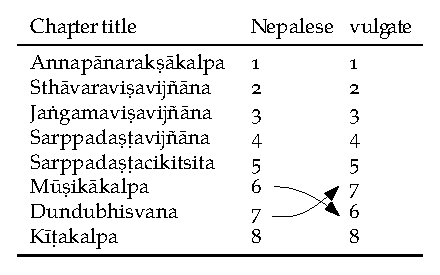
\includegraphics[width=0.65\linewidth]{chapters/media/kalpa}
%    \begin{tabular}{lll}
%    \emph{Chapter title} & \emph{Nepalese} & \emph{vulgate}   \\
%    \toprule
%      Annapānarakṣākalpa   &  1 &  1 \\
%     Sthāvaraviṣavijñāna & 2 &  2\\
%     Jaṅgamaviṣavijñāna &  3 & 3 \\
%     Sarppadaṣṭavijñāna & 4  &  4 \\
%     Sarppadaṣṭacikitsita & 5 & 5 \\
%     Mūṣikākalpa &  {6} & \textbf{7} \\
%     Dundubhisvana & {7} & \textbf{6} \\
%     Kīṭakalpa & 8 & 8 \\
%    \bottomrule  
%    \end{tabular}
\end{table}

% TODO: \usepackage{graphicx} required
%\begin{figure}
%    \centering
%    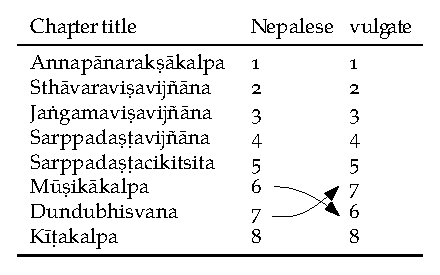
\includegraphics[width=0.65\linewidth]{chapters/media/kalpa}
%    \caption{}
%    \label{fig:kalpa}
%\end{figure}

\noindent
This difference in sequence does not have an immediately obvious 
significance.
            \thispagestyle{empty}
        % !TeX root = incremental_SS_Translation.tex
\section{Kalpasthāna, adhyāya 1}

\subsection{Literature}

A brief survey of this chapter's contents and a detailed assessment of the
existing research on it to 2002 was provided by Meulenbeld.\footcite[IA,
289--290]{meul-hist} Translations of this chapter since 2000 have appeared by 
\textcites[131--139]{wuja-2003}[3, 1--15]{shar-susr}{srik-2002}.\footnote{For a 
bibliography of translations to 2002, including Latin (1847), English (1877), Gujarati (1963) 
and Japanese (1971), see \cite[IB, 314--315]{meul-hist}.}

More recently, a discussion of the fourth chapter of this section in the light of
the Nepalese manuscripts was published by Harimoto.\footcite[101--104]{hari-2011}
After a close comparative reading of lists of poisonous snakes, Harimoto concluded
that, “the Nepalese version is internally consistent while the [vulgate] editions
are not.”  Harimoto showed how the vulgate editions, had been adjusted textually to smooth 
over inconsistencies, and gave
insights into these editorial processes.\footnote{The two editions
 that Harimoto noted, \cite{susr-trikamji3} and \cite{bhat-1889}, present identical
texts.}



\subsection{Manuscript notes}

\begin{itemize}
    \item \MScite{Kathmandu NAK 5-333} has foliation letter numerals, for example
on f.\,323a, that are similar to \MScite{Cambridge Add.\ 1693},\footnote{Scan
at 
\href{https://cudl.lib.cam.ac.uk/view/MS-ADD-01693/1}{cudl.lib.cam.ac.uk/view/MS-ADD-01693/1}.}
 dated to 1165\,\CE\, noted in Bendall's chart of Nepalese letter-numerals \cite[Lithograph V, 
after p.\,225]{bend-budd}
\end{itemize}

\newpage

\subsection{Translation}

\begin{translation}
 \item[1--2]  And now I shall explain the procedures for safeguarding food and
drink, as were declared by the Venerable Dhanvantari.\footnote{MS H adds in the
margin \dev{atha khalu vatsa suśrutaḥ} “Now begins Vatsa Suśruta.”  This phrase
has been copied here by the scribe from the beginning of the \SS\ chapter in the
\emph{sūtrasthāna} on the rules about food and drink (\Su{1.46.3}{214}).  The
scribe presumably felt, not unreasonably, that this section had common subject
matter with the present chapter.  Further, SS 1.46.3 is the only place in the Nepalese 
transmission of the \SS\ that names Dhanvantari and integrates him into the narrative of the 
\SS\ as the teacher of Suśruta. 
  
 The mention of Dhanvantari here is the only other time in the Nepalese
transmission that this authority is cited as the source of Ayurvedic teaching, and the unique 
occurrence of this actual phrase, “as was declared by the Venerable Dhanvantari.”
See the discussion by \citet[28--32]{kleb-2021b}, who concludes that the earliest
recoverable recension of the \SS\ may have had the phrase only at this point and
not elsewhere in the work.}
 
 \item[3] 

 Divodāsa, the king of the earth, was the foremost supporter of religious
discipline and virtue. With unblemished instruction he taught his students, of
whom Suśruta was the leader.\footnote{This is a quite different statement from
the vulgate \citep[559]{susr-trikamji3} that has Dhanvantari as the teacher, and
calls him the \se{kāśipati}{Lord of Kāśī}.  Ḍalhaṇa followed the vulgate but
explicitly noted the reading before us with small differences: \dev{divodāsaḥ
kṣitipatistapodharmaśrutākaraḥ} “Divodāsa, the king of the earth, was a mine of
traditions about discipline and virtue.”}

\subsection{[Threats to the king]}

\item[4--5]  

Evil-hearted enemies who have plucked up their courage, may seek to harm the king,
who knows nothing of it.  He may be assailed with poisons by or by his own people
who have been subverted, wishing to pour the poison of their anger into any
vulnerability they can find.\footnote{Verses about the use of Venemous Virgins as a weapon
do not appear in the Nepalese manuscripts. Cf.\ \cite[81\,f., 132]{wuja-2003}.  This material 
is present in the commentary of Gayadāsa.} 

\item[6] Therefore, a king should always be protected from poison by a physician.

%A king may be cunningly assailed with poisons by evil-hearted enemies who
%have plucked up their courage, or even by his own people turned traitor,
%wishing to pour the poison of their anger into any chink they can find. Or
%sometimes by women using various concoctions, hoping to make him love
%them.\footnote{On how women of ill-character mix their nail-clippings or
%menstrual blood, etc.\ with the king's food, see
%p.\,\pageref{dusyodara}.} Or again, if a Venomous Virgin is used, a man can
%lose his life instantly.\label{visakanya}
%% \footnote{\label{visakanya}On the `Venomous
%% Virgin', see p.\,\pageref{intro:visakanya}.}

\item [7] 

The racehorse-like fickleness of men's minds is well known. And for this reason, a
king should never trust anyone.\footnote{The verb \root śvas is conjugated as a
first class root in the Nepalese manuscripts.}

\item [8--11]

He should employ a doctor in his \se{mahānasa}{kitchen} who is respected by experts, who 
belongs to a good family, is orthodox, sympathetic, not emaciated, and always busy.

\item [12--13]

The kitchen should be constructed at a recommended location and orientation.  It should
have a lot of light,\footnote{We read \dev{mahacchuciḥ} with the Nepalese manuscripts and 
against the vulgate's \dev{mahacchuci}.  We understand \dev{śucis} as a neuter noun 
meaning “light” following \citet[1050a]{apte-prac}.} have clean utensils and be staffed by 
men 
and
women who have been vetted.\footnote{Verses detailing the ideal staff are omitted in the 
Nepalese manuscripts. 
Cf.\ \cites[560]{susr-trikamji3}[132]{wuja-2003}.}


\item[17--18ab]

The chefs, \se{voḍhāra}{bearers}, and makers of boiled rice soups and cakes and whoever
else might be there, must all be under the strict control of the
doctor.\footnote{The word \dev{saupodanaikapūpika} “chefs for the boiled rice soups
and cakes” is grammatically interesting.  The term \dev{sūpodana} (as opposed to
sūpaudana) is attested in the \emph{Bodhāyanīya\-gṛhyasūtra} 2.10.54 
\citep[68]{shas-1920}.  More pertinently, perhaps, \dev{sūpodana} is attested in
the Bower Manuscript, part II, leaf 11r, line 3 \citep[vol.\,1,
p.\,43]{hoer-bowe}.} 
% 2.11.54 supodana in the Bodh. (from Einoo's cards)
% sūpodana kṣīrodana
% Bower MS 328
% Kāty  otoṣthayoḥ samāse vā.

\item[18cd--19ab]

An expert  knows people's \se{iṅgita}{body language} 
through abnormalities
in voice, movement and facial expression. He should be able to identify 
a poisoner by the following signs.\q{Cf.\ Arthaśāstra 1.21.8.}


\item[19cd--23]

Wanting to speak, he gets confused, when asked a question, he never arrives at an
answer, and he talks a lot of confused nonsense, like a fool.  He laughs for no
reason, cracks his knuckles and scratches at the ground. He gets the shakes and
glances nervously from one person to another. His face is drained of colour, he is
\se{dhyāma}{grimy} and he cuts at things with his nails.\footnote{The word
\dev{dhyāma} is glossed by Ḍalhaṇa (in a variant reading) as someone who is the
colour of dirty clothes \Su{5.1}{560}.}  A poisoner goes the wrong way and is
absent-minded.

\item[25--27]

I shall explain the signs to look for in toothbrush twigs, in food and drink as
well as in \se{abhyaṅga}{massage oil} and \se{avalekhana}{combs}; in
\se{utsādana}{dry rubs} and showers, in \se{kaṣāya}{decoctions} and 
\se{anulepana}{massage ointment};
in \se{sraj}{garlands}, clothes, beds, armour and ornaments; in slippers and footstools, and
on the backs of elephants and horses; in \se{snuff}{nasya}, \se{dhūma}{inhaled
    smoke}, \se{añjana}{eye make-up}, etc., and any other things which are commonly 
    poisoned. Then, I shall also explain the remedy.

\item[28]

% My old Susruta.tex translation has \bird and \animal commands for making 
% indexes.  Convert them to the \se{}{} command that we're using in the 
% present document.
\newcommand\animal[4]{\se{#2}{#1}} 
\let\bird=\animal 

%28
Flies or crows or other creatures that eat 
a poisonous \se{bali}{morsel} served 
from the king's portion, die on the spot. 

\item [29] 

Such food makes a fire crackle violently, and gives it an overpowering colour like
a peacock's throat.

\item[30--33]

%Its flames sputter, it has acrid smoke, and before long it goes out. 

After a chukar partridge %\animal{chukar partridge}{cakora}{Alectoris
% chukar}{Collins 45}
looks at food which has poison mingled with it, its eyes are promptly drained of
colour; a peacock pheasant %\animal{peacock pheasant}{jīvajīvaka}{Polyplectron
% bicalcaratum}{Dave BSL 270, 273,
%274, 281}
drops dead.  A koel %\animal{koel}{kokila}{Eudynamys scolopacea}{Collins 66}
changes its song and the common crane %\animal{common crane}{kroñca}{Grus
% grus}{Collins 47}
rises up excitedly.\footnote{The verb \dev{arcchati} “rises up” is a rare form
best known from epic Sanskrit \citep[see][212, \S 7.6.1]{ober-2003}.   The
transmitted form \dev{kroñca} is obviously a colloquial version of Sanskrit
\dev{krauñca}.  Commenting on \Su{1.7.10}{31}, Ḍalhaṇa interestingly gives the
colloquial versions of several Sanskrit bird names, even singling out
pronunciation in the specific location of Kānyakubja.  For \dev{krauñca} he says
that people pronounce it \dev{kurañja} and \dev{koṃci}.  The form \dev{koñca}
is found in Pāli (see \cite[731]{cone-dict}, who notes that Ardhamāgadhī has the
same form). Elsewhere, Ḍalhaṇa calls the bird \dev{krauñcira},  \dev{krauñci}, and 
\dev{kaicara}
(\Su{1.46.105}{223}, \Su{6.31.154}{684} and
(\Su{6.58.44}{790} respectively).}  It will excite a peacock 
%\bird{peacock}{mayūra}, %{Pavo cristatus}{Collins 39}
and the terrified parakeet %\saneng{parakeet}{śuka}%{Psittacula krameri\slash
% eupatria\slash
%cyanocephala}{Collins 64}
and the hill myna %\ssaneng{hill myna}{sārikā}%{Acridotheres tristis tristis, L.,
% etc.}{Ali \#1006,
%\citet[28\,ff.]{Dave}, \citet[119]{Collins}}
screech. The swan %\animal{swan}{haṃsa}{?}{?}
trembles very much, and the racket-tailed drongo %\animal{racket-tailed
% drongo}{bhṛṅgarāja}{Dicrurus paradiseus}{Collins 123}
churrs.\footnote{Ḍalhaṇa seemed confused about the \sed{bhṛṅgarāja}{racket-tailed
drongo}.  He called it a generic \sed{bhramaraka}{drongo}, a word that can also mean 
“bee,” \citep[62]{dave}, and then said that it is like the
\sed{dhūmyāṭa}{black drongo} \citep[for a nice explanation of this name,
see][62--63]{dave} and that people call it “the king of birds.”} The chital deer
%\saneng{pṛṣaṭa}{chital}  
sheds tears and the
monkey releases excrement.\footnote{\MScite{Kathmandu KL 699} reads 
\sed{vṛṣabha}{bull} for
\sed{pṛṣata}{Chital deer}.  The latter may perhaps be mistaken for the former in
the Newa script, although the reading of \MScite{Kathmandu KL 699} is hard to 
read at this point.}

\item[34]

Vapour rising from tainted food gives rise to a pain in the heart,
it makes the eyes roll, and it gives one a headache.\footnote{ “Tainted” translates
\dev{upakṣipta}.  The word's semantic field includes “to hurl, throw against,” and
especially “to insult verbally, insinuate, accuse.”  The commentator Ḍalhaṇa
glossed the term as, “spoiled food given to be eaten” (\dev{vidūṣitasyānnasya
bhoktuṃ dattasya}), but he noted that some people read “\dev{ukhākṣipta}” or
“thrown into a pan.”  Other translators have commonly translated it as “served,” perhaps
influenced by Ḍalhaṇa's “\sed{datta}{given}.”}


\item[35, 36cd] 

In such a case, an errhine and a collyrium that are costus, \se{lāmajja}{lāmajja
    grass}, \se{nalada}{spikenard} and \se{madhus}{honey};\footnote{The vulgate 
    supplies another phrase and verb at this point that is not present in the Nepalese 
    transmission, but that makes the text flow more easily.}  a paste of sandalwood
on the heart may also provide relief.\footnote{\citet[350]{sing-1972} discussed
the difficulties in identifying \dev{lāmajja}, a plant cited more often in the
\SS\ than in the \CS; Ḍalhaṇa adopted the common view that it is a type of \emph{uśīra} or 
vetiver grass.  The grammatical neuter form 
\dev{madhus}  “sweetness” of the Nepalese
manuscripts is less common than neuter \dev{madhu} “honey, sweetness,
liquorice.”}

\item[37]

Held in the hand, it makes the hand burn, and the nails fall out. In such a case,
the \se{pralepa}{ointment} is \se{śyāmā}{beautyberry}, %{Callicarpa macrophylla,
% Vahl.}{AVS 1.334,    NK \#420},
\se{indragopa}{velvet-mite}, %{Kerria lacca
% (Kerr.)}{http://www.icar.org.in/ilri/de fault.htm},
soma and \se{utpala}{water-lily}.%
%{Nymphaea stellata, Willd.}{GJM 528, IGP 790; Dutt 110, NK \#1726}
\footnote{“Beautyberry” (\emph{Callicarpa macrophylla} Vahl.) is one
identification of \dev{śyāmā}, but vaidyas and commentators have different ideas
about the plant's identity (see \cites[410]{sing-1972}[1:
334]{avs}[\#420]{nadk-1954}).  On translating \dev{indragopa} as “velvet-mite,”
see \cite{lien-1978}. Ḍalhaṇa's remarks show that he had a reading
\dev{indrāgopā} before him, and he tries to explain \dev{indrā} and \dev{gopā} as
separate plants.  But he also says that some people read \dev{indragopa}.  Ḍalhaṇa
curiously parses the name \dev{somā} (f.) out of the compound; this feminine noun
is almost unknown to Ayurvedic literature.  Some dictionaries and commentators
consider it a synonym for \dev{guḍūcī}, others for \dev{brāhmī} or
\dev{candrataru}.  Ḍalhaṇa also mentions that some people think the word refers to
the \sed{somalatā}{soma creeper}, which might explain his choice to take the word as
feminine.  But the compounded word is far more likely to be \dev{soma} (m.), the
well-known mystery plant \citep[see][76--78, 125]{wuja-2003}.  If this can be
taken as rue (\emph{Ruta graveolens}, L.), as some assert, one can point to a
pleasing passage in Dioscorides where rue plays an antitoxic role: “\ldots it is a
counterpoison of serpents, the stinging of Scorpions, Bees, Hornets and Wasps; and
it is reported that if a man be anointed with the juice of the Rue, these will not
hurt him; and that the serpent is driven away at the smell thereof when it is
burned; insomuch that when the weasel is to fight with the serpent she armeth
herself by eating Rue, against the might of the serpent.” \parencites[cited 
from][262]{wren-1956}[not found in][]{osba-dios}.}
     
     \item [38--39] If he eats that food, through inattention or by mistake, then
his tongue will feel like a \se{aṣṭhīlā}{pebble} and it will lose its sense
of taste. It stings and %\sskt{stings}{tudyate},
burns, and his \se{śleṣman}{saliva}\label{saliva} dribbles out.\footnote{The word
\dev{aṣṭhīlā} is normally feminine.   The Nepalese manuscripts read it with a
short \dev{a-} ending.  Gayadāsa noticed that some manuscripts read 
\dev{aṣṭhīla}
with a short \dev{-a} ending (\MScite{Bikaner RORI 5157}, f.\,5v:7--8) and
Ḍalhaṇa reproduced his observation.  The vulgate reading “\sed{cāsyāt}{from his
mouth}” is more obvious (\emph{lectio facilior}), but is not attested in the
Nepalese manuscripts.} In such a case, he should apply the treatment prescribed
above for vapour, and what will be stated below under “toothbrush
twigs”.\footnote{Poisoned toothbrushes are discussed in verses 48\,ff.\ below.}
     
     \item[40]
     
     On reaching his stomach, it causes \se{mūrcchā}{stupor}, vomiting, the hair
stands on end, there is distension, a burning feeling and an impairment of
the senses.\footnote{I translate \dev{mūrcchā} in the light of the metaphors
discussed by \citet{meul-2011}, that include thickening and losing
consciousness.}

     \item[41] 
     
In this case, vomiting must quickly be induced using the fruits of
\se{madana}{emetic nut}, %{Randia dumetorum, Lamk.}{NK \#2091},
\se{alābu}{bitter gourd}, %{Lagenaria vulgaris, Seringe.}{NK \#1419},
\se{bimbī}{red gourd}, %{Coccinia indica, W. \& A.}{PVS 1994.4.715; NK 534}
and \se{koṣītakī}{luffa}, %{Luffa cylindrica, (L.) M. J. Roem.
% \textnormal{or}
% L. acutangula, (L.) Roxb.}{ADPS 252, NK \#1514 etc.}
taken with milk and \se{udaśvit}{watered buttermilk}, or alternatively with
rice-water.
     
     \item[42]
     
    
 Reaching the \se{pakvāśaya}{intestines}, it causes a burning feeling, stupor,
diarrhoea, thirst, impairment of the senses, \se{āṭopa}{flatulence} and it makes
him pallid and thin.
    
    % % % % % % % % % % % % % % % % % % % % %
    
      \item [43]
In such a case, purgation with the fruit of \se{nīlī}{indigo}, 
       %{Indigofera tinctoria, L.}{NK \#1309},
together with ghee, is best.  And  `\se{dūṣīviṣāri}{slow-acting poison antidote}'
should be drunk with honey and \se{dadhi}{curds}.\footnote{The `slow-acting
poison' is discussed at \Su{5.2.25\,ff.}{565}.}
     
     \item[44]
     
     When poison is in any liquid substances such as milk, wine or water, there are
     various streaks, and foam and bubbles form.  

     \item[45]
     
     \q{I'm still unhappy about this verse.} And no reflections are visible or,
however, if they can be seen once more, they are distorted, fractured, or
tenuous and distorted too.\footnote{Both Nepalese witnesses read
\se{vikṛta}{distorted} twice, which is tautologous.  In the first occurrence
both read \dev{vikṛtā} without proper termination.  One might read the sandhi
in the second occurrence as \se{vāvikṛtā}{or not distorted}, but this gives
no better sense. The scribe of \MScite{Kathmandu NAK 5-333}, apparently the
original hand,  added in the margin the alternate reading
“\se{yamalā}{double}” as in the vulgate. Perhaps the scribe too was troubled
by the tautology.  It is also evidence that he was aware of a witness with
variant readings similar to the vulgate. We emend for grammar but retain the
\emph{lectio difficilior}.} \q{Mention this in the introduction as an example
    of the scribe knowing the vulgate.}
     
\item[46]

Vegetables, soups, food and meat are soggy and tasteless.  They seem to go stale
suddenly, and they have no aroma.\q{fn about sadyas+}  

\item[47] 

All edibles lack aroma, colour or taste.  Ripe fruits rapidly \se{pra\root
    kuth}{rot} and unripe ones ripen.\footnote{The root \root\dev{kuth} “stink, 
    putrify, rot” 
    is apparently known only from its few uses in the \SS.}

\item[48]

When a toothbrush twig has poison on it, the bristles are corroded and the
flesh of the tongue, gums and lips swells up.\footnote{Gayadāsa and Ḍalhaṇa 
point out that “\sed{dantaveṣṭa}{enclosure of a tooth}” and 
“\sed{dantamāṃsa}{flesh of the tooth}” have the same meaning 
(\Su{2.16.14--26}{331--332}).}

\item[49]

 Then, once his swelling is 
 lanced, one should \se{pratisāraṇa}{rub} it with
 \se{dhātakīpuṣpa}{fire-flame bush flowers},
 %{Woodfordia fruticosa (L.) Kurz}{AVS 5.412, NK \#2626}
 %{Terminalia chebula Retz.}{NK \#2451}, 
 \se{jambū}{jambul},
 %{Syzygium cumini, (L.) Skeels}{ADPS 188, NK \#967, Potter 168}
 \se{āmrāsthi}{mango stones} and
 \se{harītakī}{chebulic myrobalan}
 fruit mixed with honey.\footnote{This recipe is different from the vulgate.}
 
 \item[50] Alternatively, the \se{pratisāraṇa}{rubbing} can be done with either
 the roots of \se{aṅkolla}{sage-leaved alangium}, the bark
of \se{saptachada}{blackboard tree} or \se{śirīṣamāṣaka}{siris 
seeds}.\footnote{The 
    spelling of
the name \dev{aṅkolla} varies \dev{aṅkoṭa, aṅkoṭha, aṅkola} 
\citep[5]{sing-1972};
Ḍalhaṇa notes that the form  \dev{aṅkolla} is a colloquialism
(\Su{1.37.12}{161}).  The sentence is awkward and we have emended
\dev{śirīṣamāṣaka} to be a plural, as in the vulgate, rather than the ablative 
singular of 
the Nepalese witnesses.  We follow Ḍalhaṇa in interpreting the compound to refer 
to the distinctive bean-like siris seeds, rather than to \sed{māṣaka}{mung 
beans} (\Su{5.1.50}{562}).}

\item[51ab] 
 
One should give advice about a poisoned tongue-scraper or 
\se{kavala}{mouthwash} in the
same way as  for a toothbrush twig.

\item[51cd]

Massage oil that has been laced with poison is slimy, thick and discoloured.   

\item[52]

When the massage oil has been contaminated with poison, boils arise, pain, a 
\se{srāva}{discharge}, inflammation of the
skin, and sweating.\footnote{The feminine \dev{sphoṭā} for “boils” is 
unattested.} And the \se{māṃsa}{flesh} splits open.

\item[53--54]

In such a case, sandalwood, \se{tagara}{Indian rose-bay},\footnote{Some say
\dev{tagara} is Indian valerian, but there remain many historical questions about
the ancient and regional identities of this plant \citep[see, e.g., 
][173-174]{sing-1972}[334]{avs}.} costus, and \se{uśīra}{vetiver
    grass}, \se{veṇupatrikā}{bamboo leaves} , \se{somavallī}{heart-leaved 
    moonseed}
and \se{amṛtā}{calamine lotion} \se{śvetā}{white clitoria}, \se{padma}{sacred
    lotus}, and \se{kālīyaka}{Indian barberry} should be made into an
\se{anulepana}{ointment} for the patient, who has been sprinkled with cold 
water.
That is also recommended as a drink with the juice and leaves of
\se{kapittha}{wood apple}.\footnote{This compound could be interpreted as 
“wood
apple juice and \se{patra}{cassia cinnamon}.”  Note that this recipe is differs
from that of the vulgate, which requires urine.}
 
 \item[55]
 
In the case of a \se{utsādana}{dry rub}, a \se{parīṣeka}{shower}, an infusion, a
\se{anulepana}{massage ointment}, or in beds, clothes, or armour, the remedy is
the same as for \se{abhyaṅga}{massage}.
 
 
 
    \end{translation}

   
   


            \thispagestyle{empty}
        % !TeX root = incremental_SS_Translation.tex
\newcommand{\plant}[4]{#1 (\emph{#2})\footnoteA{#3; see #4}}
\let\chemical = \plant
\newcommand{\skt}[2]{#1 (\emph{#2})}
\newcommand{\sskt}[2]{\empty}
%

\chapter{Kalpasthāna 2: Poisonous Plants}

\section{Introduction}

This section begins with several lists of poisonous plants.  The Sanskrit names
for these plants are mostly not standard or familiar from anywhere in Sanskrit or
ethnobotanical literature.  It remains a historical puzzle why these particular
names are so difficult to interpret. However, we are not the first to encounter
these difficulties. In the twelfth century, the learned commentator on the text,
Ḍalhaṇa, remarked,
\begin{quote}
In spite of having made the greatest effort, it has been impossible to identify
these plants. In the Himalayan regions, Kirātas and Śabaras are able to identify
them.\footnote{After \SS, \emph{kalpasthāna} 2.5 \citep[564]{vulgate}. From the
view of Sanskrit authors, Kirāṭas and Śabaras were tribal peoples.  The
eleventh-century author Bhikṣu Govinda, however, cast his treatise as a dialogue 
with a
Kirāṭa king called Madana who was a master of the alchemical art \citep[IIA,
620]{meul-hist}.}
\end{quote}
Ḍalhaṇa also recorded variant readings of these poison names from the manuscripts
that he consulted of the lost commentary of Gayadāsa (fl.\ c.\ \AD\ 1000). The
identities of these poisons have been in doubt for at least a thousand
years.\footnote{See \cite[80--81]{wuja-2003}.}  Identifications have in many cases
    been equally impossible for us today.

One path for exploration in this situation is to attempt to reverse-engineer some 
identifications by considering the known toxic plants of India.\footnote{Valuable 
reference sources on Indian plant toxicology in general include 
\cite[chs.\,10, 11]{pill-2013} and \cite[parts 1.II, 3 and 4]{barc-2008}.}

%\section{Manuscript notes}

\section{Literature}

Meulenbeld offered an annotated overview of this chapter and a bibliography
of earlier scholarship to 2002.\fvolcite{IA}[290--291]{meul-hist} 

\section{Translation}

\begin{translation}
    
    \item[1]
    And now I shall explain \diff{what should be known} about stationary 
    poisons.\footnote{No reference is made to Dhanvantari 
    \citep[see][]{birc-2021}. “Stationary” here is a term contrasted with “moving,” 
    and signifies plants as opposed to animals and insects.}
  
    \item[3]
    \noindent It is said that there are two kinds of poisons,
    \se{sthāvara}{stationary} and \se{jaṅgama}{mobile}. The former
    dwells in ten sites, the latter in sixteen places.
   
    \item[4]
    Traditionally, the ten are: root, leaf, fruit, flower, bark,
    \se{kṣīra}{milky sap}, \se{sāra}{pith}, \se{niryāsa}{resin}, the
    elements (\emph{dhātu})\sse{dhātu}{element}, and the tuber.

    \item[5]
    
    In that context,\label{poisonousplants}
    \begin{itemize}
        \item the eight root-poisons are:\footnote{Some South Asian plants with
    poisonous roots that we would have expected to see in this list include
    \emph{Croton tiglium}, L., \emph{Calotropis} spp., \emph{Citrullus colocynthus} L. 
    Schrad., and \emph{Ricinus
    communis} L.\ \citep{pill-2010}.} 
%    \q{Expected \citep{pill-2010}:\\ Croton
%        tiglium, L. = Naepala, Jayapala, kanakaphala, titteriphala (NL \#720);
%        Calotropis spp.;\\ Citrullus colocynthus (colocynth);\\ Ricinus communis
%        (castor); }
        \begin{enumerate}
        \item  \gls{klītaka},\footnote{Liquorice eaten in excess can be poisonous, but it is 
        unlikely to be the plant intended here.  \citet[124]{gvdb} noted that the 
        poisonous 
        root mentioned in this passage, “remains to be idenitified.”}
       
        \item \gls{aśvamāraka},\footnote{The roots of sweet-scented oleander 
        are highly toxic, as are most parts of the plant \citep{pill-2019}.}
    
        \item \gls{guñjā},\footnote{Jequirity contains a dangerous
        toxin called Abrin in its seeds and to a lesser extent in its leaves,
        but apparently not in its roots or bulb. Abrin is not harmful if eaten,
        but an infusion of the bruised (not boiled) seeds injected or rubbed in
        the eyes can be fatal \citep[\# 6]{NK}.  The dose can be quite small.}
        
        \item \diff{\gls{subhaṅgurā}},\footnote{The plant is
usually called just \emph{bhaṅgurā} without the prefix \emph{su-} “good.”  However, there 
is no reported toxicity associated with \emph{E. prostrata}.  The vulgate reads 
\dev{sugandhā} (\gls{sugandhā}).}
        
       \item \diff{\gls{karaṭā}},\footnote{This poisonous root cannot at present
be securely identified.  Similar-sounding candidates include \emph{karkaṭaka},
\emph{karahāṭa} (emetic nut), and \emph{karaghāṭa}, but since this is a
prose passage, there would be no reason to alter the word to fit a metre.
\citet[255]{moni-sans} cite an unknown lexical source that equates
\emph{karaṭa} (mn.) with safflower (\emph{Carthamus tinctorius}, L.), but
this plant does not have a poisonous root.} 
%
%        \item \plant{luffa}{gargaraka $\rightarrow$ garāgarī?}{Luffa echinata,
%        Roxb.}{NK
%            \#1517},
and ending with 
%
\item \gls{vidyutśikhā},%
%%\plant{leadwort}{vidyutśikhā $\rightarrow$ agni- or
%    rakta-śikhā?}{Plumbago zeylanica (or rosea?), L.}{NK \#1966, 
%    1967}
\footnote{The roots of both rose and white leadwort are very toxic.} 

\item \diff{\gls{anantā} (?)},\footnote{The text reads masculine
    \emph{ananta}, which is not a plant name.  Gayī's commentary on
    \Su{5.2.5}{564} noted a variant reading of feminine \emph{anantā} in
    place of \emph{gargaraka}, earlier in the compound. But the feminine
    \emph{anantā}, \gls{anantā}, is not a poisonous plant.} and

\item \gls{vijayā2},\footnote{\citet[61, n.\,3]{meul-sear} argued that our text
    reads a masculine or neuter noun \emph{vijaya}, which never signifies cannabis.
    However, unlike the vulgate, the unanimous readings of the Nepalese manuscripts
    give feminine \emph{vijayā}.  Nevertheless, even the feminine form only started to
    signify \emph{Cannabis sativa} L. after the end of the first millennium
    \citep{meul-sear,wuja-cann,mchu-2021}. The \emph{Sauśrutanighaṇṭu} gives 
    a 
    number
    of synonyms for \emph{vijayā}, almost none of which have any poisonous parts
    \citep[5.77, 10.143]{suve-2000}.  But one of them, \emph{viṣāṇī} (also
    \emph{meṣaśṛṅgī}), is sometimes equated with \emph{Dolichandrone falcata (DC.)
    Seemann} \citep[518]{adps}, a plant used as an abortifacient and fish poison
    \citep[\#862]{NK}.  This identification is tenuous.} 
    %
    %        \footnote{Large doses of the root-extract of rauwolfia can be fatal.
    %
    %        In large doses luffa is emetic and a drastic purgative. }
        \end{enumerate}
        \end{itemize}
    
        \item
        the leaf-poisons include:
             \begin{itemize}            
        \item \gls{viṣapatrikā},
        \item \diff{\gls{lambaradā}},
%        \item \plant{`choice tree'}{varadāru}{unknown}{?},
        \item \gls{karambha},
        and
        \item big \gls{karambha};
            \end{itemize}

        \item
        the fruits of items like:
        \gls{guñjā},
        \gls{aruṣkara},
        and
        \gls{viṣavedikā}
        are
                    \begin{itemize}
         \item \diff{\plant{kumudavati}{kumadavati}{unknown}{?}},
         
        \item \diff{\plant{reṇuka}{?}{?}{Piper aurantiacum Wall.\ 
        \citep[\#1924]{NK} is 
        not poisonous.}},
%        \plant{`little bamboo'}{veṇukā}{Bambusa bambos, Druce?}{NK 
%        \#307},

\item
\diff{\plant{kurūkaka}{?}{?}{?}},

\item
\diff{\plant{`little bamboo'}{veṇuka}{Bambusa bambos, Druce?}{NK 
           \#307}},\footnote{Not poisonous.},

        \item \plant{thorn apple}{karambha}{Datura metel, L.}{AVS 2.305 (cf.\
            Abhidhāna\-mañjarī), NK \#796\,ff., Potter 292\,f., ADPS 132.}, 
        
        \item 
            \plant{`big
            thorn apple'}{mahākarambha}{Datura metel, L.?}{AVS 2.305 (cf.\
            Abhidhāna\-mañjarī), NK \#796\,ff., Potter 292\,f., ADPS 132.},

\item 
\diff{\plant{`pleaser'}{nandanā}{?}{?}},

\item 
\diff{\plant{`crow'}{kāka}{?}{?}},
        
%        \item \plant{ribbed gourd}{karkoṭaka}{Luffa acutangula, (L.) Roxb.? 
%        (Mormodica
%            cochinchinensis, Spreng.? Cf.\ Luffa tuberosa)}{AVS 3.347 (NK \#1640,
%            1643; NK \#1520)}, 
        
%        \item \plant{black cardamom}{hareṇu}{Amomum 
%            subulatum,
%            Roxb.?}{PVS Caraka 2.734, AVS 1.128, NK \#154}, \item \plant{purple
%            calotropis}{khadyotaka $\rightarrow$ arka?}{Calotropis gigantea, (L.) R.
%            Br.}{ADPS 52, AVS 1.341, NK \#427, Potter 63},
%        \item \plant{carmarī}{carmarī}{unknown}{?}, \item 
%        \plant{heliotrope}{ibhagandhā
%            $\rightarrow$ hastiśuṇḍa?}{Heliotropium indicum, L.}{AVS 3.136, NK
%            \#1203},
%        \item \plant{`snake-killer'}{sarpaghāti}{unknown}{?},
%        \item \plant{`gladdener'}{nandana}{unknown}{?}, and
%        \item \plant{`juice-cooker'}{sārapāka}{unknown}{?};\footnote{Bamboo 
%is 
%        not 
%        toxic.
%        Heliotrope flowers are abortifacient in large doses.}
            \end{itemize}
    
        \item
        the flower-poisons include those of:
              \begin{itemize}
            
        \item \plant{rattan}{vetra}{Calamus rotang, L.}{AVS 1.330, NK \#413},
        \item \plant{wild chinchona}{kādamba}{Anthocephalus cadamba, Miq.}{NK 
        \#204},
        \item \plant{black pepper}{vallīja $\rightarrow$ marica}{Piper
            nigrum, L.?}{NK \#1929; Rā.6.115, Dha.4.85, Dha.2.88},
        \item \plant{thorn apple}{karambha}{Datura metel, L.}{AVS 2.305
            (cf.\ Abhidhāna\-mañjarī), NK \#796\,ff., Potter 292\,f., ADPS 132.},
        and
        \item \plant{big thorn apple}{mahākarambha}{Datura metel, L.?}{AVS 
        2.305
            (cf.\ Abhidhāna\-mañjarī), NK \#796\,ff., Potter 292\,f., ADPS 132.};
            \end{itemize}
        
        \item
        the seven bark, \se{sāra}{pith} and \se{niryāsa}{resin} poisons are:
              \begin{itemize}
            
        \item \plant{`gutboiler'}{antrapācaka}{unknown}{?},
        \item \plant{`blade'}{kartarīya}{unknown}{?},
        \item \plant{wild mustard}{saurīyaka}{Cleome viscosa, L.?
            (cf.\ Rā.4.144)}{AVS 2.116, NK \#615},
        \item \plant{emetic nut}{karaghāṭa $\rightarrow$ karahāṭa? $\rightarrow$
            madana}{Randia dumetorum, Lamk.}{NK \#2091},
        \item \plant{thorn apple}{karambha}{Datura metel, L.}{AVS 2.305
            (cf.\ Abhidhāna\-mañjarī), NK \#796\,ff., Potter 292\,f., ADPS 132.},
        \item \plant{wild asparagus}{nandana $\rightarrow$ 
        bahuputrā?}{Asparagus 
        racemosus,
            Willd.}{ADPS 441, AVS 1.218, NK \#264, IGP 103,
            IMP 4.2499ff., Dymock 482ff.},
        and
        \item \plant{munj grass}{nārācaka}{Saccharum bengalense, Retz.?}{NK
            \#2184};\footnote{The bark of wild asparagus (\emph{Asparagus 
            racemosus}, Willd.)
        is toxic.}
            \end{itemize}
        \item
        the three \se{kṣīra}{milky sap}-poisons are:
              \begin{itemize}
            
        \item \plant{purple calotropis}{kumudaghnī $\rightarrow$ arka?}{Calotropis
            gigantea, (L.) R. Br.}{ADPS 52, AVS 1.341, NK \#427, Potter
            63},\footnote{The name of this poison, \emph{kumuda-ghnī}, means 
            `lotus
        killer'.  In Sanskrit literature, the \emph{kumuda} lotus is associated
        with the moon, since it blossoms by night.  Since the sun causes this lotus
        to close, it is therefore an `enemy' of the lotus.  One of the chief words
        for the sun, \emph{arka}, is also the name of \emph{Calotropis gigantea},
        which indeed has a milky juice which is a violent purgative, poison and
        abortifacient.}
        \item \plant{oleander spurge}{snuhī}{Euphorbia neriifolia, L., 
        \textnormal{or}
            E. antiquorum, L.}{ADPS 448, AVS (2.388), 3.1, NK
            \#988, IGP 457b},
        %   \marginpar{`The milky juice or gum which flows from the branches
        %     [of \emph{E. antiquorum}] is an acrid irritant\ldots. Internally it is a
        %     powerful emetic and a violent purgative, even in very small quantities'.
        %     --- NK \#982}
        and
        \item \plant{`web-milk'}{jālakṣīri}{unknown}{?};
            \end{itemize}
        
        \item
        the two \se{dhātu}{element}-poisons are:
              \begin{itemize}
            
        \item \plant{`foam-stone'}{phenāśma}{unknown}{?}, and
        \item \plant{orpiment}{haritāla}{Arsenii trisulphidum}{NK v.\,2,
            p.\,20\,ff.};\footnote{\citet[38--42]{dutt-1922} conjectured that
        `foam-stone' may be impure white arsenic obtained by roasting orpiment.}
            \end{itemize}
        \item
        the thirteen tuber-poisons are:
        \begin{itemize}
             \item \plant{jequirity}{kālakūṭa}{Abrus
            precatorius, L.? Cf.\ RRS 21.14.}{AVS 1.10, NK \#6, Potter
            168.},\footnote{The much later (perhaps sixteenth century) alchemical
        \emph{Rasa\-ratna\-samuccaya} of pseudo-Vāgbhaṭa (21.14) says that the
        \emph{kāla\-kūṭa} poison, here translated as `jequirity', is similar to
        `\emph{kāka\-cañcu}' or `Crow's Beak', which is indeed a name for the
        plant jequirity or
        \emph{Abrus precatorius}, L., more commonly called \emph{guñjā} (not to
        be confused with \emph{gañjā}). The black seed-pod is described as
        having a `sharp deflexed beak' in botanical descriptions, so the
        Sanskrit name is quite graphic and appropriate. The poisonous scarlet
        seeds of \emph{A. precatorius} can have a distinct black dot or tip,
        which could perhaps be translated `\emph{kāla-kūṭa}', or `Black Tip'.
        
        The \emph{Rāja\-nighaṇṭu\-pariśiṣṭa} (9.35) gives \emph{kālakūṭaka} as a
        synonym for \emph{kāras\-kara}, or \emph{Strychnos nux-vomica}, L., 
        whose
        seeds are notoriously poisonous.}
        \item \plant{wolfsbane}{vatsanābha}{Aconitum napellus, L.}{AVS 1.47,
            NK \#42, Potter 4\,f.},
        \item \plant{Indian mustard}{sarṣapa}{Brassica juncea, Czern. \&
            Coss.}{AVS 1.301, NK \#378},
        \item \plant{leadwort}{pālaka $\rightarrow$  citraka}{Plumbago zeylanica
            (indica? rosea?), L.}{Rā. 6.124, ADPS 119, NK \#1966,
            1967},
        \item \plant{`muddy'}{kardama}{unknown}{?}, the
        \item \plant{`Virāṭa's plant'}{vairāṭaka}{unknown}{?},
        \item \plant{nutgrass}{mustaka}{Cyperus rotundus, L.}{ADPS 316,
            AVS 2.296, NK \#782},
        \item \plant{atis root}{śṛṅgīviṣa}{Aconitum heterophyllum, Wall.
            ex Royle}{AVS 1.42, NK \#39},
        % \item \plant{liquorice}{prapuṇḍarīka $\rightarrow$ 
        %madhuka?}{Glycyrrhiza
        %  glabra, L.}{AVS 3.84, NK \#1136},\footnote{Non-toxic.}
        \item \plant{sacred lotus}{prapuṇḍarīka}{Nelumbo nucifera, Gaertn.}{Dutt 
        110, 
        NK
            \#1698}, \item \plant{radish}{mūlaka}{Raphanus sativus, L.}{NK 
            \#2098},
        \item \plant{`alas, alas'}{hālāhala}{unknown}{Cf. Soḍhalanighantu p.43 
        (sub
            bola) = stomaka = vatsanābha}, \item \plant{`big
            poison'}{mahāviṣa}{unknown}{?}, and \item 
            \plant{galls}{karkaṭa}{Rhus
            succedanea, L.}{NK \#2136}.\footnote{Leadwort root is a powerful poison.
        Nutgrass is tuberous, but non-toxic. Atis has highly toxic tuberous
        roots. Neither sacred lotus nor galls are toxic. The `alas, alas' poison
        (\emph{hālāhala}) is the mythical poison produced from the churning of
        the ocean at the time of creation: it occurs in medical texts such as
        the present one, and commentators identify it with one or other of the
        lethal poisons such as wolfsbane or jequirity.
        \citet[126]{agra-indi} makes the intriguing suggestion
        that the word \emph{hālāhala},
        possibly to be identified with Pāṇini's \emph{hailihila} (P.6.2.38),
        may be of Semitic origin, although his evidence
        seems uncertain (\citet[1506a]{stei-pers} cites Persian \emph{halāhil}
        `deadly (poison)' as a loan from Sanskrit). \cite[iii.585]{mayr-kurz}
        also cites a claim for an Austro-Asiatic origin for the word.}
            \end{itemize}

    Thus, there are fifty-five stationary poisons.
    
    \item[6] There are believed to be four kinds of wolfsbane, two kinds of
\emph{mustaka}, and six kinds of Indian \emph{sarṣapa}.  But the rest are said
to be unique types.
    
    
    
    \subsection{The effects of poisons}
    \item[7--10]
    
People should know that root-poisons cause \se{udveṣṭana}{writhing}, 
\se{pralāpa}{ranting}, and
\se{moha}{delirium}, and  leaf-poisons cause yawning, writhing, and 
\se{śvāsa}{wheezing}.
    
 Fruit-poisons cause swelling of the
   scrotum, a burning feeling and writhing.  Flower-poisons will
    cause vomiting, \se{ādhmāna}{distension} and \se{svāpa}{sleep}.  
    
The consumption of poisons from bark, \se{sāra}{pith} and \se{niryāsa}{resin} 
will
cause foul breath, \se{pāruṣya}{hoarseness}, a headache, and a
discharge of \se{kapha}{phlegm}.\footnote{At \Su{1.2.6 }{11}, Ḍalhaṇa
glosses \se{pāruṣya}{hoarseness} as \emph{vāgrūkṣatā}, “a rough, 
dry voice.”}
    
    % 10
    
     The \se{kṣīra}{milky sap}-poisons make one froth at the mouth,  cause loose
stool, and make the tongue feel heavy.\footnote{At \Su{6.54.10}{773}, Ḍalhaṇa
glosses \se{viḍbheda}{loose stool} as \emph{dravapurīṣatā}, “having liquid
stool.” }  The \se{dhātu}{element}-poisons give one a crushing pain in the
chest, make one faint and cause a burning feeling on the palate.
    
    % 11
    These poisons
    are classified as ones which are generally speaking lethal after a period of time.
    
    \item[11--17]
    
    \subsubsection{Symptoms of tuber poisoning}
    The tuber-poisons, though, are severe.  I shall talk about them in detail.
    
    %12
    
    With
    \plant{jequirity}{kālakūṭa}{Abrus precatorius, L.?
        Cf.\ RRS 21.14.}{AVS 1.10, NK \#6, Potter 168.}, there is numbness
    and very severe trembling.
    %shivering
%
    With
    \plant{wolfsbane}{vatsanābha}{Aconitum napellus, L.}{AVS 1.47,
        NK \#38, Potter 4\,f.}, there is rigidity of the neck, and the faeces,
    and urine become yellow.
    
    %13
    With \se{sārṣapa}{sārṣapa}%
%With \plant{Indian mustard roots}{sārṣapa}{Brassica juncāea, Czern \&
%    Coss.}{AVS 1.301, NK \#378}
,\footnote{\emph{Sārṣapa} would normally mean
“connected with mustard,” and excessive consumption of mustard oil can be 
harmful. However, the \emph{Sauśrutanighaṇṭu} (156) gives
\emph{rakṣoghnā} as a synonym for \emph{sarṣapā}. This can be
\textit{Semecarpus anacardium}, L.f., which has some poisonous parts.} the
\skt{wind becomes defective}{vātavaiguṇya}, there is \se{ānāha}{constipation},
and \se{granthi}{lumps} start to appear. %
With \plant{leadwort}{pālaka $\rightarrow$  citraka}{Plumbago zeylanica
    (indica? rosea?), L.}{Rā. 6.124, ADPS 119, NK \#1966, 1967}, there is weakness
in the neck, and speech gets jumbled.\footnote{The verse in the Nepalese version 
ends with a plural verb that does not agree with the dual of the sentence subject.}
    
    %14
    With the one called
    \plant{`muddy'}{kardama}{unknown}{?},
    there is a \se{praseka}{discharge}, the faeces pour out, and  the eyes
    turn yellow.
    %
The
    \plant{`Virāṭa's plant'}{vairāṭaka}{unknown}{?}
causes pain in the body and illness in the head.
    %
    Paralysis of one's arms and legs and trembling are said to be caused by
    \se{mustaka}{mustaka}.%
%    \plant{nutgrass}{mustaka}{Cyperus rotundus, L.}{ADPS 316, AVS 2.296,
%        NK \#782} %
\footnote{The substitution 
    in \MScite{NAK 5-333} affecting 15cd is caused by an eye-skip to the word 
    \emph{viṣeṇa} in 2.17.  \emph{Mustaka} commonly refers to Cyperus 
    rotundus, L.; the root is used in āyurveda but is 
    not poisonous.  However other dictionaries list \emph{mustaka} amongst 
    serious poisons, for example \emph{Rājanighaṇṭu} (22 v.\,42) and 
    \emph{Rasaratnasamuccaya} 16, v.\,80.  However, its ancient identity is still 
    doubtful.}
    \item[ 15b]
    With \se{mahāviṣa}{great aconite}\q{-> ativiṣa}
%    \plant{atis root}{śṛṅgīviṣa}{Aconitum heterophyllum, Wall.
%        ex Royle}{AVS 1.42, NK \#39}, 
    one's limbs grow weak, there is a burning
    feeling and swelling of the belly.\footnote{The poisonous root 
    \se{mahāviṣa}{great poison} is not clearly identifiable, although \emph{viṣa} 
    is commonly aconite.  Verse 6 above notes that there are several kinds of 
    aconite.}
    \item[ 16a]
    With \se{puṇḍarīka}{puṇḍarīka},
%    \plant{sacred lotus}{puṇḍarīka}{Nelumbo nucifera, Gaertn.}{Dutt 110,
%        NK \#1698},
    one's eyes go red, and one's belly becomes distended.\footnote{The word 
    \emph{puṇḍarīka} very commonly means sacred lotus, Nelumbo nucifera, 
    Gaertn. The entire plant is edible and cannot be the poison intended here.  
    \citet[252]{gvdb} noted that this poison is unidentified and that it is also 
    listed as a poison in \Cs{ci.23.12}{}.}\q{Look up the ca. reference.}
    \item[ 16b]
    With \se{mūlaka}{mūlaka},
%    \plant{radish}{mūlaka}{Raphanus sativus, L.}{NK \#2098}es,
    one's body is drained of colour and the limbs are paralysed.\footnote{The word 
    \emph{mūlaka} very commonly means the radish, \emph{Raphanus sativus}, 
    L. The root is edible and cannot be the poison intended here.  
    \citet[317]{gvdb} noted that this poison is unidentified.}
    
    %17
    \item[ 17a]
        
    With \se{Aconite}{hālāhala}, a man turns a \se{dhyāma}{dark colour}, and
gasps.\footnote{Identification of \emph{hālāhala} is  uncertain. It may simply
be a mythical poison, or its specific identity may have been lost over the
centuries. Late \emph{nighaṇṭu}s identify it as \emph{stomaka} =
\emph{vatsanābha}, i.e., \emph{Aconitum napellus}, L. 
(\emph{Soḍhalanighantu}
p.43). Ḍalhaṇa on \Su{5.2.17}{564} interprets our “gasps” as “the man laughs
and grinds his teeth.”  But this gloss is probably displaced and intended to apply 
to verse 2.18.}

% 5.221 Rājanighaṇṭu

\item[ 17b] With \plant{atis root}{śṛṅgīviṣa}{Aconitum
    heterophyllum, Wall.\ ex Royle}{AVS 1.42, NK \#39}, one gets violent
\se{granthi}{knots} and stabbing pains in the 
heart.\footnote{\citet[407]{gvdb} noted that \emph{vatsanābha} and 
\emph{śṛṅgīviṣa} are two different varieties of poisonous Aconites that are 
difficult to distinguish.}
    
    %18
    \item[ 18a]
    With
    \se{monkey}{markaṭa}, one leaps up, laughs, and 
    bites.\footnote{\citet[299]{gvdb} said of \emph{markaṭa}, “an 
    unidentified vegetable poison.”  Cf.\ \cite[v.36]{suve-2000} for synonyms that 
    lead to the non-toxic jujube tree.}
    
    %{galls}{karkaṭa}{Rhus succedanea, L.}{NK \#2136}
    
    \item[ 18b-19a]
%    Experts said that the thirteen cited highly potent tuber-poisons should be 
%known to have possessed ten features:
%    %()Experts said that one should know that these thirteen cited highly potent 
%%tuber-poisons have ten features:
    %Experts said that these thirteen highly potent tuber-poisons which are 
    %mentioned here consist of ten features.)
    
    Experts have said that one should know that the thirteen highly potent 
    tuber-poisons, which are mentioned here, have ten \se{guṇa}{qualities}.
    
    \item[ 19b--20a]
    
    The ten are:
    \begin{itemize}
        \item    \se{rūkṣa}{dry}, 
        \item hot, 
        \item sharp, 
        \item \se{sūkṣma}{rarified},
        \item     fast-acting, 
        \item \se{vyavāyin}{pervasive}, 
        \item \se{vikāsin}{expansive}, 
        \item \se{viśada}{limpid},
        \item     light, and 
        \item indigestible.    
    \end{itemize}
    %20b
    \item[ 20b]
    Because of dryness, it may cause inflammation of the wind; because of heat
    it inflames the choler and blood. 
    %21
    Because of the sharpness it unhinges the
    mind, and it cuts through the connections with the \skt{sensitive
        points}{marman}.  Because it is rarified it can infiltrate and distort
    the parts of the body.\footnote{We read the active \emph{vikaroti} with 
    Ḍalhaṇa against the 
    transmitted passive \emph{vikriyeta}, since it must be the parts of the body 
    that are distorted, not the poison.}    
    

\item[22]
Because it is fast-acting it kills quickly, and because of its pervasiveness
it affects one's \skt{whole physical constitution}{prakṛti}.\footnote{Ḍalhaṇa
on \Su{5.2.22}{565} explained this as “\se{akhiladehavyāptirūpam}{takes the
form of pervading the whole body}.”}  Because of its expansiveness it enters
into the \se{doṣa}{humour}s, \se{dhātu}{bodily constiuents}s, and even the
impurities\sskt{impurity}{mala}.  Because it is limpid it overflows, and
because it is light it is difficult to treat.  Because it is indigestible it
is hard to eliminate.  Therefore, it causes suffering for a long time.
    
    \item[ 24]
    Any poison that is instantly lethal, whether it be
    stationary, mobile, or artificial, will be known to 
    have all ten of these qualities.
    
    
  
    
    \subsection{Slow-acting poison}
    \item[25cd--26]  
    \begin{verse}
        A poison that is old or destroyed by
        anti-toxic medicines, or else dried up by blazing fire, wind, or sunshine, or
        which has just lost its qualities by itself,\footnote{Ḍalhaṇa specified that this 
        refers to the ten 
        qualities that are mentioned above (\Su{5.2.26}{565}).} becomes a 
        \skt{slow-acting poison}{dūṣīviṣa}.\footnote{Ḍalhaṇa cited this verse at 
        \Su{1.46.83}{222} while explaining \emph{dūṣīviṣa}.}
                Because it has lost its potency it is
        no longer perceived.  Because it is surrounded by \se{kapha}{phlegm} it 
        has an aftermath that lasts for a very long time.
        
        \item[27] If he is suffering from this, the colour of his stools changes,
he gets sourness and a bad taste with great thirst. Stammering and close
to death, wandering about, he may feel faint, giddy, and
aroused.\footnote{Similar symptoms of slow-acting poison are described at
\Su{2.7.11--13}{296} in the context of  \se{duṣyodara}{contamination
dropsy}.  This this may explain why the vulgate inserted reference to this
disease at this point.}
        
        
        
%        Also, he has
%        the symptoms of \skt{contaminated
%            dropsy}{duṣyodara}.
%        \footnote{\label{dusyodara}`Contaminated dropsy'
%        (\emph{duṣyodara} or \emph{dūṣyudara}) is described elsewhere as a
%        condition which arises when women of ill-character mix nail clippings,
%        hair, urine, faeces, or menstrual blood with a man's food, in order to
%        gain power over him (2.7.11--13).}



        \item[28]
        If it lodges in his \se{āmāśaya}{stomach}, he becomes sick because of wind 
        and phlegm; if it lodges in his \se{pakvāśaya}{intestines}, he becomes sick 
        because of  wind and 
        choler.  A man's hair and limbs fall away and he looks like a
        bird whose wings have been chopped off.
        \item[29a--c]
        If it lodges in one of the body tissues such as 
        \se{rasa}{chyle}, it causes the diseases arising
        from the body tissues, that have been said to be wrong.\footnote{The 
        expression \emph{ayathāyathoktān} “stated to be unsuitable” is hard to 
        understand here, but is clearly transmitted in the Nepalese version.}
        and it rapidly becomes inflamed on days that are nasty
        because of cold and wind.
        
        \item[29d--31] Listen to its initial \se{liṅga}{symptoms}: it causes
heaviness due to sleep, yawning, \se{viśleṣa}{disjunction} and
\se{harṣa}{horripilation} and a \se{aṅgamarda}{bruising of the
    limbs}.\footnote{Ḍalhaṇa \Su{5.2.30ab}{565} glossed “disjunction” as the
loss of function of the joints in regard to movement.} Next, it causes
\se{annamada}{intoxication from food} and indigestion, \se{arocaka}{loss
    of appetite}, the condition of having a \se{koṭha}{skin disease} with
\se{maṇḍala}{round blotches},\footnote{The last ailment could perhaps be
ringworm.} % 5.2.31
\diff{\se{kṣaya}{dwindling away} of flesh}, swelling of the feet, hands, and
face, \diff{the fever called \textit{pralepaka}}, vomiting and
diarrhoea.\footnote{The \emph{pralepaka} fever was described by Ḍalhaṇa,
at \Su{6.39.52}{675}, as an accumulation of phlegm in the joints.  Its
symptoms are described in 6.39.54} The slow-acting poison might cause
\diff{wheezing, thirst and fever, and it might also cause distension of the
abdomen.}
        
        %Perhaps his colour may drain away and he may faint or have \se{viṣamajvara}{irregular fever}.  It may cause heightened,
        %powerful thirst.
        
        \item[32]
 
            These various disorders are of many different types: one poison may 
            produce
            madness, while another one may cause \se{ānāha}{constipation}, and 
            yet
            another may ruin the semen. One may cause \diff{emaciation}, while 
            another
            \se{kuṣṭha}{pallid skin disease}.
 
    \end{verse}

    
    \item[33]  
Something is “corrupted” by repetitively keeping to bad locations, times,
  foods, and sleeping in the daytime.  Or, traditionally, “corrupting poison” 
  (\se{dūṣī-viṣa}{slow-acting poison}) is so called because
    it may corrupt (\emph{dūṣayet}) the \se{dhātu}{body tissue}s.  
    
    
    
    
    
    \item[34-]
    \subsubsection{The stages of toxic shock}
    \label{stagesofshock}

    In the first shock of having taken a stationary poison, a person's tongue becomes dark brown and stiff, he grows faint, and panics.
    
    
    
    % FROM HERE Harṣal 35-38
    \item[35]
    In the second, he trembles, feels exhausted, has a burning feeling, as well as a
    sore throat.  When the poison reaches the \se{āmāśaya}{stomach}, it causes
    pain in the \se{hṛd}{chest}.
    
    
    
    \item[36]
    In the third,his palate goes dry, he gets violent \se{śūla}{pain} in the 
    \se{āmāśaya}{stomach}, and his eyes become weak, swollen and yellow.

    \item[37]
    In the fourth shock, it causes the intestines and stomach to
    \se{sāda}{be exhausted}, he gets hiccups, a cough,  a rumbling in the
    \se{antra}{gut}, and his head becomes heavy too.
    
     \item[38]
    In the fifth he dribbles \se{kapha}{phlegm}, goes a bad colour,
    his \diff{\se{parśvabheda}{ribs crack}},  all his humours are irritated, and he
    also has a pain in his \se{pakvādhāna}{intestines}.
   
   
    \item[39a]
    In the sixth, he loses consciousness and he completely loses
    control of his bowels.
    
    \item[39b]
    In the seventh, there are breaks in his shoulders, back and loins, and he  
stops breathing.\footnote{%
%In \Su{1.15.24}{72}, Ḍalhaṇa glossed 
%\emph{kriyā-sannirodha} 
%as “cessation of the activities of the body, speech and mind” 
%(\emph{kriyāṇāṃ kāyavāṅmānasīnāṃ sannirodhaḥ}), while 
Here at \Su{5.2.24}{566} Ḍalhaṇa glossed \emph{sannirodha} as
“complete cessation, i.e., of breath” (\emph{sannirodhaḥ 
samyaṅnirodhaḥ, ucchvāsasya iti śeṣaḥ}).
The manuscripts all read \emph{skanda} where \emph{skandha} must be 
intended; this confusion is known from Buddhist Hybrid Sanskrit 
\citep[608]{edge-1953}.}
    
    % next  40-44
    
    
    \subsubsection{Remedies for the stages of slow poisoning}
  \label{dusivisa}
  
    \item[40] In the first shock of the poison, the physician should make the man,
who has vomited and been sprinkled with cold water, drink an
\se{agada}{antidote} mixed with with honey and ghee.
    
    \item[41a] In the second, he should make the man who has vomited and been
purged drink as before;
    
    \item[41b]
    on the third, drink an antidote and a beneficial
    \se{nasya}{nasal medicine} as well as an \se{añjana}{eye salve}.
    
    
    \item[42a] In the fourth, the physician should make him drink an antidote that
is salt with a little oil.\footnote{At \Su{6.52.30}{769} Ḍalhaṇa noted that
\emph{sindhu} can be interpreted as \se{saindhava}{salt}.}
    
    

    
    \item[42b]
    In the fifth, he should be prescribed the antidote together with a
    \se{kvātha}{decoction} of honey and
    \gls{madhuka}.
   
   
    \item[43] \diff{In the sixth, the \se{siddhi}{cure} is the same as
    for diarrhoea. %
    And in the seventh, he perishes}.\footnote{The vulgate text here is quite
    different, recommending that the patient have medicated powder blown up
    his nose. It may be possible to detect the evolution of the Nepalese
    \dev{avasīdet} to the vulgate's \dev{avapīḍaś}.  The vulgate version is
    hard to construe, and we see Ḍalhaṇa struggling to interpret it in his
    commentary on \Su{5.2.43ab}{566}.  This sternutatory is, however,
    recommended in the Nepalese version at \Su{5.5.30ab}{576}, for the
    seventh shock of poisoning by a \se{rājimat}{striped snake}.  It is
    possible the text migrated from  that location to this.

\label{kakapada} Another difference at this point is that the Nepalese
version also does not support the vulgate's passage on the
\se{kākapada}{crow's foot} therapy \citep[145, n.\,106]{wuja-2003}.  The
same is the case at \Su{5.5.24}{575} and the clear description at
\Su{5.5.45}{577}, in neither of which is the therapy supported in the
Nepalese version.  This therapy seems unknown to the Nepalese
transmission.  The therapy may have migrated into the vulgate \SS\ from
the \CS\ \Ca{6.23.66--67}{574}.}
    
    % he should have medicated powder blown up his nose, 

%    and
%    after having a `\se{kākapada}{crow's foot}' cut made on his head, he
%    should have a piece of bloody meat put on
%    it.\footnote{\label{su:kakapada}Suśruta explains the term \emph{avapīḍa}
%    `medicated nasal powder' as the procedure either of administering
%    \se{avapīḍa}{nasal drops}, or blowing medicated powder into the nose
%    (4.40.44--46): it is particularly recommended for unconscious or incapable
%    patients.  The `crow's-foot' procedure is also recommended later in the
%    `Section on Procedures' (5.5.24a) in cases of snake-bite. It is also
%    described by Caraka (see p.\,\pageref{sa:kakapada} below).}
%

\item[44] 

\diff{In between any one of these shocks}, once the above treatment has been done, he
should give the patient the following cold \se{yavāgū}{gruel} together with ghee and 
honey, that will take away the poison.
       
    \item[45--46]
    
        A \se{yavāgū}{gruel} made of the following items in a
\se{niḥkvātha}{stewed juice} destroys the two poisons:
\gls{kośavatī},\footnote{At \Su{4.10.8}{449} Ḍalhaṇa glossed
    \dev{kośavatī} as \dev{devadālī} and at \Su{4.18.20}{472} as
    \dev{kaṭukośātakī}, vocabulary pointing to \emph{Cucumis cylindrica},
    \emph{Cucumis actangula} or \emph{Luffa echinata}. See glossary under
    \gls{koṣītakī}.} \gls{agnika},\footnote{A plant often cited in \SS,
        but rarely in \CS\ \citep[4]{gvdb}.  Ḍalhaṇa glossed it here,
        \Su{5.2.45}{566}, as \emph{ajamodā}, \gls{ajamodā},  but noted that
        others consider it to be \emph{moraṭa}, \gls{moraṭa}. There is
        considerable complexity surrounding the identification of
        \emph{moraṭa/mūrvā} and related synonyms \citep[314-316]{gvdb}. Taking
        \emph{agnika} as a short reference to \emph{agnimantha}, often
        identified  as \gls{agnimantha}, might be plausible, since that is
        antitoxic or anti-inflammatory, but such a short reference is not
        known elsewhere.} \gls{pāṭhā}, \gls{sūryavallī},\footnote{At
            \Su{5.2.45}{566} Ḍalhaṇa said that this plant has leaves like the
            \emph{paṭola}, \gls{paṭola}, \citet[280, 443]{gvdb} argued plausibly
            that this is a synonym for \emph{arkapuṣpī}, \gls{arkapuṣpī}, as
            Ḍalhaṇa also stated in \Su{1.45.120}{206}, and the leaves of
            Holostemma and Trichosanthes are indeed strikingly similar.  The
            appearance of the plant, a creeper with sun-like flowers, fits the
            name.  But there remains much controversy about the identities of
            these candidates \citep[e.g.,][195--198]{adps}.} %
            % got to here Dominik -
            %
            %    $\rightarrow$ jīvantī?}{Holostemma ada-kodien,
            % Schultes}{ADPS 195,
            %AVS
            %    3.167, NK \#1242, IMP 3.1619},
            \gls{amṛtā}, \gls{abhayā} \gls{śirīṣa}, and \gls{śelu},
            \gls{kiṇihī}, \diff{the two kinds of
                \gls{haridrā}},\footnote{I.e., \gls{haridrā} and \gls{dāruharidrā}.} and
                the two kinds of \gls{bṛhatī},\footnote{I.e., \gls{bṛhatī} and
                    \gls{kṣudrā}.} \gls{punarnavā}, \gls{hareṇu}, \diff{the
                        \gls{tryūṣaṇa}}, %
                    the two kinds of
                    \gls{sārivā}\footnote{I.e., \gls{anantā} and
                        \gls{pālindī}.} %
                        \diff{and \gls{utpala}}.
  \end{translation}

\newpage

    \subsection{The invincible ghee}
    
  \begin{translation}
    
    \item[ 47--49]
    
    \label{ajeya} There is a famous ghee called \se{ajeya}{“Invincible”}. It
rapidly destroys all poisons but is itself unconquered. It is prepared with a
\se{kalka}{mash} of the following plants: %
\gls{madhuka},
\gls{tagara},
\gls{kuṣṭha},
\gls{bhadradāru},
\gls{hareṇu},
\diff{\gls{mañjiṣṭhā}},
\gls{elā}
and \gls{elavālu},
\gls{nāgapuṣpa},
\gls{utpala},
\gls{sitā},
\gls{viḍaṅga},
\gls{candana},
\gls{patra},
\gls{priyaṅgu},
\gls{dhyāmaka},
the two turmerics,\footnote{I.e., \gls{rajanī} and \gls{dāruharidrā}.}
the two Indian nightshades,\footnote{I.e., \gls{bṛhatī} and \gls{kṣudrā}.}
the two kinds of \gls{sārivā},\footnote{I.e., \gls{anantā} and \gls{pālindī}.}
\gls{aṃśumatī},
and 
\diff{\gls{balā}}.
    
    \end{translation}

    \subsection{Curing the `slow-acting' poison}
    

\begin{translation}    
    
    \item[ 50--52]
    
        Someone suffering from “\se{dūṣīviṣa}{slow-acting poison}” should be well
        sweated, and purged both top and bottom.  Then he should be
        made to drink the following \diff{eminent} antidote which removes “slow-acting
        poison:”
    
    Take
    \gls{pippalī},
    \gls{dhyāmaka},
    \gls{māṃsī},
\diff{\gls{lodhra}, \gls{elā}},
\gls{suvarcikā},
\gls{bālaka}, 
\gls{gairika}, as well as \gls{hema},
and
\gls{paripelavā}.

This antitoxin, taken with honey, eliminates slow-acting poison. It is called the
“\se{dūṣīviṣāri}{enemy of slow-acting poison},” and it is not prohibited in other situations.
    
    % Deepro - 
    
    \item[ 53--54]
    If there are any other \se{upadrava}{side-effects}, such as fever, a burning
    feeling, hiccups, \se{ānāha}{constipation}, depletion of the semen,
    distension, diarrhoea, fainting, skin problems,
    \se{jaṭhara}{bellyache}, madness, trembling, then one
    should treat each one in its own terms,  using anti-toxic
    medicines.
    
    \item[ 55] For a prudent person, the slow-acting poison can be \se{sādhya}{cured}
immediately.  It is \se{yāpya}{treatable} if it is of a year's standing. Other
than this, it should be avoided for the person who eats unwholesome things.

    \end{translation}


\endinput 
% PLANTS OF GARDEN OR WOODS
% WITH POISONOUS ROOTS AND STEMS
% Arisaema triphyllum
% Colchicum autumnale
% Convallaria majalis
% Dicentra spp.
% Gloriosa superba
% Hyacinthus spp.
% Iris spp.
% Narcissus spp.
% Ornithogalum umbellatum
% Phytolacca americana
% Podophyllum peltatum
% Jack-in-the-pulpit
% Autumn Crocus
% Lily-of-the-Valley
% Bleeding-heart and
% Dutchman’s Breeches
% Glory-lily
% Hyacinth
% Iris, Flags
% Narcissus, Daffodil
% Star-of-Bethlehem
% Pokeweed
% May-apple, Mandrake
%--  DONALD WYMAN
%http://arnoldia.arboretum.harvard.edu/pdf/articles/1966-26--a-few-poisonous-plants.pdf
 % needs work on plant names
            \thispagestyle{empty}
        % !TeX root = incremental_SS_Translation.tex
\section{Kalpasthāna, adhyāya 3}

\subsection{Introduction}

\subsection{Translation}

\begin{translation}
    \item[1]
And now we shall explain the \se{kalpa}{rule} that is the required knowledge about mobile
poisons.\footnote{In contrast to stationary, plant poisons.  No reference is made to 
Dhanvantari \citep[see][]{birc-2021}.}\q{Come back to the issue of "kalpa".  Look up 
passages in the Kośa.}

\item[2] 

\item[3] 

The full explanation about the sixteen \se{adhiṣṭhāna}{carriers} of the mobile
poisons, that have been mentioned by me in brief, will be stated.


\footnote{ “Carrier” for \se{adhiṣṭhāna}{base, foundation} 
 tries to capture the idea that the author will describe the creatures in which poisons inhere.} 
 
 \item[4]
 In that context, they are: 
 \begin{itemize}
     \item sight and breath,
     \item teeth and nails,
     \item \diff{mouth},
     \item  urine and faeces,
     \item \diff{menstrual blood},
     \item semen,
     \item \diff{penis},
     \item saliva,
     \item \diff{lethal points},
     \item \se{mukhasaṃdaṃśā}{nipping with the mouth},
     \item \se{avaśardhita}{fart},\footnote{This interpretation comes from
     Ḍalhaṇa on \Su{5.3.4}{567}, but he reads \dev{viśardhita}.}
     \item \diff{anus},\footnote{Ḍalhaṇa on \Su{5.3.4}{567} noted this reading.}
     \item bones,
     \item bile,
     \item \se{śūka}{bristles},
and 
     \item corpses.
     
     \end{itemize}
    
    \item[5] TBA
    
    \item [6]
    \diff{The enemies of the king pollute the 
    waters, roads and foodstuffs 
    in enemy territory. The experienced physician, 
    who has learned how to purify things, 
    should clean up those polluted things.} 
    
    \item[7]
    
    Polluted water is slimy and smells of tears.\footnote{\dev{asra} normally
means “tears,” but rarely means “blood.” }  It is covered with froth and
covered with streaks. The frogs and fish die, the birds are crazed and, along with
the wetland creatures, they wander about aimlessly.
    
     \item [8]
     
     Men, horses and elephants who swim in it experience vomiting, delusion,
fever, swelling and sharp pains.\footnote{On the polysemy of \se{nāga}{elephant\slash 
snake}, see \cite{seme-1979}.} 
    He should try to purify that polluted water, after curing their ailments.
     
\item [9]

And so, he should burn
    \gls{dhava}  and 
    \gls{aśvakarṇa}, % Dipterocarpa turbanitus Gaertn., GVDB 28
        as well as
    \gls{pāribhadra}, %Erythrina suberosa, GVDB 245
        with
    \gls{pāṭalā} % GVDB 242 Stereospermum suaveolens DC.
        and 
    \gls{sidhraka} % 
        and 
   \gls{muṣkaka}, % GVDB 312, Schrebera swietenioides Roxb and 
   %Elaeodendron glaucum Pers.
        and with
    \gls{rājadruma} % āragvadha, GVDB 37 Cassia fistula Linn
        and 
    \gls{somavalka}.
Then he should sprinkle that ash, cold, on the waters.

\item [10--11]

And in the same way, putting a handful of the ash in a pot, one may also purify water that 
one wants.

If any one of the limbs of cows, horses, elephants, men or women, touch a place on
the ground that enemies have spoiled with poison, or a ford or rock or a flat
surface, then it swells up and burns and its hair and nails fall out on that
place.\footnote{``Swells up" translates an unclear reading that was probably
    \dev{śūyati}, which may be an irregular form of $\surd$\dev{śū, śvā, śvi} 
    \citep[see][175--176]{whit-root}.}

\item [12]

In that situation, he should grind up \gls{anantā} together with all the aromatic
items, with alcoholic drinks.  And then  he should sprinkle the paths that need to
be used with waters mixed with mud.\footnote{Our “alcoholic drinks” translates
    \dev{surā}.  For a discussion of this term at our period see \cite[37--39
    \emph{et passim}]{mchu-2021a}.} \diff{And if there exists another path, he should 
    go by
    that.}\footnote{Ḍalhaṇa on \Su{5.3.12}{568} cited a similar reading for the fourth
        pāda, but with a negative particle,  “and if there is no other way, one should go
        by that.”}
    
    

\item [13]

When grasses and foods are polluted, people collapse, fall unconscious. And others
vomit. They get \se{viḍbheda}{loose stool} or they die.
%\footnote{In “they get
%loose stool,” the verb \dev{ārcchanti} ($\surd$\dev{ṛ}), transmitted in both
%Nepalese manuscripts, has an irregular initial strong vowel.  Alternatively, and perhaps
%more likely, it is a combination of \dev{ā+$\surd$ṛ}, 
%conjugated unusually as a class 6 verb, but with an appropriate sense of “to fall into 
%(misfortune).”} 
One should apply to them the therapy as described.

\item [14--15]

Alternatively, one should wipe various musical instruments with antidotes that
remove poison and then play them.   What is called the most excellent paste for a
musical instrument is \gls{tārāvitāra}\footnote{“Certain minerals” translates
    \dev{tārāvitāra}, the unanimous reading of the Nepalese witnesses.  But the
    meaning of this expression is not clear and may even refer to plants, like the
    other ingredients.  The vulgate reads \dev{tāraḥ sutāraḥ}, which is also not very
    clear.  However, Ḍalhaṇa on \Su{5.3.14}{568} identified these as “silver” and
    “mercury.” This is highly unlikely to be a correct understanding of the \SS\
    passage.  Historically, mercury is not naturally present in the South Asian
    peninsula \pvolcite{5}[233]{watt-1896}, and the word \dev{pārada} that Ḍalhaṇa
    used is probably a loan-word from Persian \citep[sub \emph{paranda,
    parranda}][244b]{stei-pers}.  Mercurial compounds are not reliably attested in
    South Asia until two or three centuries after the composition of the \SS.  The
    currently available “śāstric” recension of the \emph{Arthaśāstra} that is datable
    to 175--300 \CE\ \citep[29--31]{oliv-2013} does not mention mercury (\emph{ibid},
    534).  See further the study by \citet[17, \emph{et passim}]{wuja-2013b}.} 
    together with \gls{surendragopa}, and a portion of of \gls{kuruvinda} equal to
    that, together with the bile called “brown cow”.\footnote{\dev{surendragopa} and
        \dev{kuruvinda} are both uncertain, see index. Ḍalhaṇa's opinion has been followed
        here, but it seems fair to say that all commentators were guessing.} By the sound
        of the musical instrument, even terrible poisons that may be present at that place
        are destroyed.
        
\item[16]

If there is smoke or wind that is affected by poison then birds are dazed and fall
to the ground.  People get coughs, colds, and head illnesses, and acute eye
diseases.\footnote{The syntax of this verse is somewhat loose; the vulgate has
    regularized it, smoothing out the difficulties.}

\item[17]

The smoke and air can be purified by putting 
\gls{lākṣā},
\gls{haridrā},
\gls{ativiṣā},
and
\gls{abhayā},
with
\gls{vakra},
\gls{kuṣṭha},
\gls{elā},\footnote{}\q{write footnote:  don't repeat ativiṣā; vulgate similar to H.}
and
\gls{hareṇu},
and
\gls{priyaṅgu} into the air.



\end{translation}
            \thispagestyle{empty}
        % !TeX root = incremental_SS_Translation.tex
\section{Kalpasthāna, adhyāya 4}

\subsection{Introduction}
The fourth chapter of the Kalpasthāna of the \emph{Suśrutasaṃhitā} addresses 
the topic of snake bites and snake venom.  Unusually for the Nepalese version of 
the \SS, the discussion is framed as a question from Suśruta to the wise 
Dhanvantari.  Suśruta's questions are about the number of snakes, how they 
are classified, the symptoms of their bites and the pulses or stages of poisoning 
experienced by a victim of snakebite and related topics.  The taxonomy of snakes 
is presented in a presentational variant form in Figure~\ref{snakes}.


    
\subsection{Literature} 

A brief survey of this chapter's contents and a detailed assessment of the
existing research on it to 2002 was provided by Meulenbeld.\footcite[IA,
292--294]{meul-hist} There also exists a herpetological literature from
colonial India as well as more recent studies of snakes in the context of
religious life.\footnote{E.g., \cite{ewar-1878, wall-1921}. 
    \citet[75--124]{wall-1913} provided a useful analysis of the medical effects
    of snake envenomation in India arranged by the varied symptomology of
    different snakes.  He also discussed the difference between toxic effects
    and fright (69--75) and also the difficulties arising out of uncertainty
    about the effects of snake-bite (124--126).  \citet{doni-2015} provided a
    good survey of snakes as protagonists in religious literature from the
    \emph{Atharvaveda} through the epics, \emph{Purāṇas} and Buddhist
    literature. \citet[31--33 \emph{et passim}]{slou-2016} discussed the \SS's
    \emph{Kalpasthāna} as a precursor and influence on later Tantric traditions
    of snake-bite interpretation and therapy. } %
    %Translations of this chapter
    % since 2000 have appeared by
    %\textcites[131--139]{wuja-2003}[3,
    % 1--15]{shar-1999}{srik-2002}.\footnote{For a
    %    bibliography of translations to 2002, including Latin (1847),
    % English
    % (1877),
    %Gujarati (1963)
    %    and Japanese (1971), see \cite[IB, 314--315]{meul-hist}.}
    
A discussion of this chapter specifically in the light of the Nepalese
manuscripts was published by Harimoto.\footcite[101--104]{hari-2011} After a
close comparative reading of lists of poisonous snakes, Harimoto concluded
that, “the Nepalese version is internally consistent while the [vulgate]
editions are not.”  Harimoto showed how the vulgate editions had been
adjusted textually to smooth over inconsistencies, and gave insights into
these editorial processes.\footnote{The two editions that Harimoto noted,
    \cite{vulgate} and \cite{bhat-1889}, present identical texts.}


\subsection{Translation}

\begin{translation}
    \item[1] Now we shall explain the \se{kalpa}{procedure} relating to the
knowledge concerning the venom in those who have been bitten by
snakes.\footnote{The \emph{Sarvāṅgasundarī}, commenting on
    \Ah{1.16.17}{246}, glossed \dev{kalpa} as \dev{prayoga}.}
    
    \item[3] Suśruta, grasping his feet, questions the wise Dhanvantari, the 
    expert in all the sciences.
    
    \item[4]
    
    “My Lord, please speak about the number of snakes, and their divisions,
the symptoms of someone who has been bitten, and the knowledge
concerning the \se{vega}{successive shocks} of poisoning”.\footnote{The
    expression “successive shocks” translates \dev{vega}, which is other
    contexts may mean “(natural) urge.”  Here, it is rather the discrete
    stages or phases of physiological reaction to envenomation.  Cf.\ the
    symptoms of cobra poisoning described by \citet[80]{wall-1913}.}
        
    \item[5]
    
    On hearing his query, that distinguished physician spoke.
    
    “The venerable snakes such as Vāsukī and Takṣaka are uncountable. 
    
\item[6--9ab]

“They are snake-lords who support the earth, as bright as the ritual fire,
ceaselessly roaring, raining and scorching. They hold up the earth, with its
oceans, mountains and continents. If they are angered, they can destroy the
whole world with a breath and a look.  Honour to them. They have no role
here in medicine.

“The ones that I shall enumerate in due order are those mundane
ones with poison in their fangs who bite humans.\footnote{The next few
    verses are discussed in detail by \citet[101--104]{hari-2011}, who shows
    that in the taxonomy of snakes, the Nepalese version of the \SS\ has greater
    internal coherence than the vulgate recension.}


\end{translation}

    \begin{figure}
        \centering
        \Tree [.Snakes{ (80)}  
        [.Darvīkara {26 kinds} ]
        [.Maṇḍalin  {22 kinds} ]  
        [.Rājimant  {10 kinds} ]   
        [.Nirviṣa     {12 kinds} ]  
    [.Vaikarañja [.{3 kinds} {7 kinds} ] ]  ]
         \caption{The taxonomy of snakes in the vulgate, \Su{5.4.9--13ab}{571}.}
         \label{snakes1}
\end{figure}
\begin{figure}
\centering          
            \Tree [.Snakes{ (80)}  
            [.Darvīkara {26 kinds} ]
            [.Maṇḍalin  {26 kinds} ]  
            [.Rājimant  {13 kinds} ]   
            [.Nirviṣa     {12 kinds} ]  
            [.Vaikarañja {3 kinds} ]  ]
        \caption{The taxonomy of snakes in the Nepalese version.}
        \label{snakes2}
        \end{figure}
    
    \begin{translation}
        \item[9cd--10]    
        
        “There are eighty kinds of snakes and they are divided in five ways:
        Darvīkaras, Maṇḍalins, Rājimants, and Nirviṣas.  And Vaikarañjas that are
        traditionally of three kinds.\footnote{\citet{hari-2011} translated these
            names as “hooded,” “spotted,” “striped,” “harmless,” and “hybrid.” Figure 
            \ref{snakes1} shows the taxonomy described in the vulgate text; Figure 
            \ref{snakes2} shows the different and more logical division of the Nepalese 
            version of the \SS.}
            
    \item [11] 
    
    “Of those, there are twenty and six hooded snakes, and the same number
of Maṇḍalins are known.\q{Or “There are 20 phaṇins and 6 maṇḍalins.  The
    same number are known. There are 13 Rājīmants.”  Or even, “there are 20
    Phaṇins and six of them are Maṇḍalins.” Are phaṇins really the same as
    darvīkaras?}  There are thirteen Rājīmants.\footnote{The phrasing of
    this śloka is awkward.}
    
    \item [12]
    
    “There are said to be twelve Niriviṣas and, according to tradition, three 
    Vaikarañjas.
    
    \item [13--14ef]
    
“If they are trodden on, bad or provoked or looking for food, those very
angry snakes will bite.  And that is said to happen in three ways:
\se{sarpita}{serpented}, \se{darita}{torn} and thirdly \se{nirviṣa}{without
    venom}.  Some experts want to add “hurt by the snake's body”.\footnote{This 
    might refer to constriction.  The phrase reads like a commentarial addition 
    rather than the main text of the \SS.}

\item[15--16]

“An aroused snake may make one, two or more deep \se{pada}{imprints} of its
teeth, without much blood.\footnote{\label{pada-snakes} The word
    \dev{udvṛtta} “aroused” was glossed by Ḍalhaṇa at \Su{5.4.15}{571} as
    \dev{unmoṭya}, a word not found as such in standard dictionaries
    (\cite{moni-sans,apte-prac,mayr-kurz,josi-maha}. Semantic considerations
    suggest that the word is not related to $\surd$\emph{muṭ} “break” or
    \emph{mūta/mūṭa} “woven basket.” Perhaps it is related to the Tamil
    \texttamil{மோடி} (\emph{mōṭi},) whose meanings include “arrogance, grandeur,
    display” \citep[\#5133]{burr-1984} or to faintly-documented forms like
    \emph{moṭyate} “is twisted” \citep[\#10186]{CDIAL}. Ḍalhaṇa's \dev{unmoṭya}
    may thus mean “twisting up” or “making an arrogant display.” \par Note that
    \dev{pada} “imprints” is being used in the same sense as in \Su{1.13.19}{57}
    when describing the marks on the body where a knife scarifies the skin
    before leeching. See footnote \ref{pada-leeches}.} They have a
    \se{cuñcumālaka}{little row of puncture-marks},\footnote{The usual
        dictionary lexeme is \dev{cañcu} “beak, billl,” not \dev{cuñcu} as in the
        Nepalese witnesses.} making them abnormal. They are close together and
        swollen.  The physician can recognize this as “\se{sarpita}{serpented}.”

    
    % 
    %https://global.oup.com/us/companion.websites/9780190200886/student/chapter10/gline/quotation/
\end{translation}
            \thispagestyle{empty}      
        % !TeX root = ../incremental_SS_Translation.tex
   
\chapter{Kalpasthāna 5: Therapy for those Bitten by Snakes}

\section{Introduction} 

\section{Literature}

A brief survey of this chapter's contents and a detailed assessment of
the existing research on it to 2002 was provided by
Meulenbeld.\footnote{\volcite{IA}[294--295]{meul-hist}. In addition to the
    translations mentioned by \tvolcite{IB}[314--315]{meul-hist}, a translation
    of this chapter was included in \volcite{3}[35--45]{shar-1999}.} 
    
    
    \newpage
    
\section{Translation}

\emph{Passage numbers refer to the canonical numbering of the vulgate edition  
\citep{vulgate}.
}
\begin{translation}
    \item [1]
    Now we shall explain the \se{kalpa}{procedure} that is the therapy for 
    someone bitten by a snake.\footnote{On \dev{kalpa}, see note 
    \ref{arunadatta:kalpa}.}
    
    \item [2]  \ \cbdelete 
       
    \item[3] For a person bitten on a limb by any snake, one should first
of all make a strong binding, at four fingers measure above the
bite.\footnote{Application of a tourniquet is deprecated by modern
    establishment medicine, which relies on antivenom medications
    \citep[e.g.,][150--151 et passim in the literature]{pill-2013}.
    
    The vulgate introduces the word \dev{ariṣṭā} at this point.  This may be a 
    borrowing from \Ca{Ci.23.251cd}{582}.}
    
    
    \item[4]
    
    Poison does not move around into the body if it is prevented by
bandages (\emph{ariṣṭā})\sse{ariṣṭā}{bandage} or by any other soft
items of \se{plota}{cloth}, \se{carmānta}{leather} or
bark.\footnote{It is hard to translate the word \dev{ariṣṭā}
    otherwise than “bandage,” as referred to by \dev{badhnīyāt} in the
    previous verse, and apparently similar to items of cloth etc., and
    called a \dev{bandha} in the next verse.  But in general Sanskrit
    literature, including medical literature, the word (in masc.\ gender)
    means either “an alcoholic tonic” or “an omen of death,”
    (\Su{1.30.3}{137}), or is a plant name.  This raises a question mark
    over its unique meaning in the present context.  The \AH\
    (\Ah{Utt.36.42cd}{910}) seems to be a gloss on \dev{ariṣṭā}, saying
    “An expert in mantras may bind using a braid made of silk etc.,
    empowered with mantras” (see also \Su{5.5.8}{575}).}
    
\item[5] Where a \se{bandha}{bandage} is not suitable, one should
\diff{raise the bite up} and then cauterize it.\footnote{The vulgate
    reads \dev{utkṛtya} “having excised” rather than translate \dev{uddhṛtya}
    “having raised up.”} Suction, cutting and cauterizing are recommended in
    all cases.

\item[6] Suction will be good after filling the mouth with
\diff{\se{pāṃśu}{earth}}.\footnote{The vulgate recommends cloth, not
    earth (\Su{5.5.6}{574}).}  Alternatively, the snake should be bitten
    \diff{by the person who knows} that they have just been
    bitten.\footnote{The syntax is odd here, and the vulgate has removed the
        difficulties. \Dalhana{5.5.6}{574} noted that one should hold the snake
        firmly and give a good bite to its head and tail
        (\dev{hastābhyāmupasaṃgṛhya pucche vaktre ca sarpaḥ samyag daṣṭavyaḥ}). 
        Our colleague Dr Madhu K. Paramesvaran reports that this procedure is
        known in Malayalam \emph{viṣavaidya} treatises and is practiced in
        Kerala, though rarely: “this practice has been described as one of the
        first-response cares for snakebite in most of the Malayalam texts of
        Vishavaidya. I have never seen this happening in real life and my
        teachers used to consider it to be a method (albeit a bit outrageously
        dangerous) for self-reassurance by the patient.” \citep{para-2023}. Cf.\
        the Viṣavaidya text edited by \citet{maha-1958}.}


\item[7] 

Now, one should in no way cauterize someone bitten by a Maṇḍalin. Because
of the over-abundance of \se{pittaviṣa}{poison in the bile}, that bite will
\diff{be lethal} as a result of cauterization.\footnote{Verses 5.4.29,
    and 37 above note that the venom of Maṇḍalins particularly irritates the
    bile.}

\subsection{[The application of mantras]}

\item [8]

An expert in mantras should tie on a \se{ariṣṭā}{bandage} too, with
mantras.  But they say that a bandage that is tied on with cords and so
on causes the \diff{poison to be purified}.\footnote{\Dalhana{5.5.8}{575}
    clarified that on the one hand the bandage must be accompanied with
    mantras, but on the other hand, it may also be used without mantras.  The
    verse seems to put two points of view.}

\item[9]

Mantrās prescribed by gods and \se{brahmarṣi}{holy sages}, that are
imbued with truth and \se{tapas}{religious power} are inexorable and they
rapidly destroy intractable poison.

\item [10]

Drugs cannot eliminate poison as quickly as the application of mantras
imbued with \se{tapas}{religious power} and imbued with truth,
\se{brahma}{holiness} and religious power.\footnote{\Dalhana{5.5.10}{575}
    noted that mantras like “kurukullā” and “bheruṇḍā” are explained in other
    treatises and therefore not explained further in his commentary. These
    two mantras are the names of tantric Śaiva and Buddhist goddesses. For a
    study on this specific subject see \citet{slou-2016b}. \volcite{IIB}[151,
    n.\,344]{meul-hist} provides a bibliography to 2002 of studies on
    Kurukullā, who is mentioned in Māhuka's \emph{Haramekhalā}, and
    \cite[30--34]{meul-2008b} includes discussion of Bheruṇḍa as a bird, with
    related terms.} 
    % and  further  studies such as \cite[ch.\,22]{shaw-2006}.

\item [11] The mantras should be received by a person who is
abstaining from women, meat and \se{madhu}{mead}, who has a
\diff{restricted} diet, and who is pure and lying on a bed of \gls{kuśa}.

\item [12]

For the mantras to be successful, one should diligently worship the
\se{devatā}{deity} with perfume, garlands, and \se{upahāra}{oblations},
as well as \se{bali}{sacrificial offerings}, and with \se{japa}{mantra
    repetition} and rituals.\footnote{\Dalhana{5.5.12}{575} noted that
    \dev{upahāra} includes incense, while \dev{bali} refers to sacrifice
    with an animal (\dev{sapaśunaivedya}).}


\item [13]

But mantras pronounced illicitly or that are deficient in
\se{svara}{accents} and letters do not give success.  So
\se{agada}{antitoxic} procedures need to be employed.

\subsection{[Blood letting]}

\item [14]

A skilled physician should puncture \diff{a \se{sirā}{duct} which is
\se{śākhāśrayā}{located on the limb}, and comes from the bite and 
the general area.} If the poison has spread, one on the forehead should be
pierced.

\item [15] 

\diff{The blood being drawn out draws away all the poison}.\footnote{The
    Nepalese version uses a present passive participle construction here,
    that is less common than the vulgate's locative absolute.  The Nepalese 
    version states that it is the blood coming out of the patient that carries away 
    the venom; the vulgate text says merely that the venom emerges while the 
    blood comes out.} Therefore one
    should cause blood to flow, for that is his very best procedure.

\item [16]  

After scarifying the area around the bite, one should smear it with
\se{agada}{antidotes} and sprinkle it with water infused with
\gls{candana} and \gls{uśīra}.\footnote{\dev{pracchāna} is the second of
    the two methods of blood letting  described in \SS\ \Su{1.14.25}{64}
    (this verse does not appear in the Nepalese version of the \SS).}

\item [17]

One should make him drink \se{agada}{antidotes} including milk, honey and 
ghee. If they are unavailable, the earth of black ants can be good. 


\item [18]

Alternatively, he should consume \gls{kovidāra}, \gls{śirīṣa} and
\gls{arka} with \gls{kaṭabhī}.

    
    %%%%%%%%%%%%
    \strut
    \bigskip
    
    \item[34] \footnote{After this verse, the vulgate text adds twelve
    verses, 35--46, that do not appear in the Nepalese version.}
    
     \item[78] \footnote{After this verse, the vulgate text adds five
        verses, 79--83, that do not appear in the Nepalese version.}
\end{translation}    
            \thispagestyle{empty}
        %d !TeX root = ../incremental_SS_Translation.tex
\chapter{Kalpasthāna 6: Mice and rats}
\label{mūṣikā}


\section{Introduction}

This chapter is numbered 6 in the Nepalese version, but 7 in the vulgate.

\subsection{Literature}

%A brief survey of this chapter's contents and a detailed assessment
%of the existing research on it to 2002 was provided by
%Meulenbeld.\footnote{\volcite{IA}[295]{meul-hist}. In addition to the
%    translations mentioned by \tvolcite{IB}[314--315]{meul-hist}, a
%    translation of this chapter was included in
%    \volcite{3}[61--66]{shar-1999}.} 



\section{Translation}

\begin{translation}
    
    \item[1] 
    
Now I shall explain the \se{kalpa}{procedure} on the topic of
\se{mūṣikā}{mice}.\footnote{The word \dev{mūṣikā} does not distinguish 
between rats and mice; the same is true for MIA and NIA derivatives
\cite[\#10258]{CDIAL}.}
    
    \item[3] 
    
    
    \end{translation}

            \thispagestyle{empty}
        %d !TeX root = ../incremental_SS_Translation.tex
\chapter{Kalpasthāna 7: Beating Drums}
\label{dundubhi}

\section{Introduction}

This chapter is numbered 7 in the Nepalese version, but 6 in the vulgate.

\subsection{Literature}

A brief survey of this chapter's contents and a detailed assessment
of the existing research on it to 2002 was provided by
Meulenbeld.\footnote{\volcite{IA}[295]{meul-hist}. In addition to the
    translations mentioned by \tvolcite{IB}[314--315]{meul-hist}, a
    translation of this chapter was included in
    \volcite{3}[61--66]{shar-1999}.} 
%    Magic practices (kṛtyā) with a drum (dundubhi) are already mentioned in 
%the
%    \emph{Atharvaveda} (5.31.7).\footnote{\volcite{IB}[400]{meul-hist}.}
%    
%    See on thedundubhi: V.R.R. Dikshitar (1987): 379-380; S.R. Kul-
%    shrestha (1994): 113-114.

\section{Translation}

\begin{translation}
    
    \item[1] 
    
Now I shall explain the \se{kalpa}{procedure} on the topic of
sounding the \se{dundubhi}{kettle drum}.\footnote{This title suggests
    that the chapter may once have begun with the words “the drums are to
    be sounded" or at least that this is the subject of the chapter
    (Pāṇini 4.3.87).
    
On the translation “kettle drum” see \cites[318]{hopk-1889}{ross-2014}.}
    
    \item[3] 
    
One should take the ash of the following items, mix it with cows'
urine and an \se{kṣāra}{caustic} compound, take an extract and cook
it thoroughly: % deep  breath ...
\gls{dhava}, \gls{aśvakarṇa}, \gls{tiniśa}, \gls{picumarda},
\gls{pāṭalī}, \gls{pāribhadraka},\footnote{\label{drum-detox}The
    ingredients to this point are similar to the water-detoxifier
    described in \SS\ \Su{5.3.9}{568}, p.\,\pageref{water-detox} above.}
    \gls{udumbara}, \gls{karaghāṭaka}, \gls{arjuna}, \gls{sarjja},
    \gls{kapītana}, \gls{śleṣmātakā}, \gls{aṅkoṭha}, \gls{kuṭaja},
    \gls{śamī}, \gls{kapittha}, \gls{aśmantaka}, \gls{arka},
    \gls{ciribilva}, \gls{mahāvṛkṣa}, \gls{arala}, \gls{madhuka},
    \gls{madhukaśigru}, \gls{śāka}, \gls{gojī},
    \gls{bhūja},\footnote{Note the unanimous Nepalese MS reading
        \dev{bhūja}, the Middle Indo-Aryan form of Sanskrit \dev{bhūrja}
        \citep[\#9570]{CDIAL}.} \gls{tilvaka}, \gls{ikṣuraka},
        \gls{gopaghoṇṭā}, and \gls{arimeda}.
     
One should add to this the powder of the following items, together
with an equal quantity of metals: \gls{pippalī}, \gls{pippalīmūla},
\gls{taṇḍulīyaka}, \gls{varāṅga}, \gls{coraka}, \gls{mañjiṣṭhā},
\gls{karañjikā}, \gls{hastipippalī}, \gls{viḍaṅga},
soot\sse{gṛhadhūma}{soot}, \gls{ananta}, soma,\footnote{The
    literature on the identification of Soma is large and continuing
    \parencites[76--78, 125--131]{wuja-2003}{clar-2017}. To the cited
    literature, the useful historical discussion by
    \citet[449--455]{gvdb} gave special attention to the āyurvedic
    literature.  Its presence in this recipe may add special value or
    power to the resulting compound.} \gls{sarala}, \gls{bāhlīka},
    \gls{kuśa}, \gls{āmra}, \gls{sarṣapa}, \gls{varuṇa}, \gls{plakṣa},
    \gls{nicula}, \gls{vardhamāna}, \gls{vañjula}, \gls{putraśreṇī},
    \gls{saptaparṇa}, \gls{ṭuṇṭuka}, \gls{elavāluka},
    \gls{nāgadantī},\footnote{\Dalhana{5.6.3}{580} glossed
        \dev{nāgadantī} as a type of \dev{indravāruṇī} (\gls{indravāruṇī}),
        but he noted that Jejjaṭa had thought it was \dev{dantī}
        (\gls{dantī}).} \gls{ativiṣā}, \gls{bhadradāru}, \gls{marica},
        \gls{kuṣṭha}, and \gls{vacā}.\footnote{\Dalhana{5.6.3}{580} noted
            that Gayadāsa omitted several of the above ingredients, keeping
            thirty.}  Once it has been brought to the boil with the alkali, one
            should take it down and place it in a iron
            pot.\footnote{\label{kṣārapāka2}\Dalhana{5.6.3}{580} explained 
            that
                the above substances, from pepper onwards, should be placed in 
                liquid
                alkali and then cooked until they are neither too runny nor too
                viscous (a phrase he copied from \Su{1.11.11}{47}).  The 
                preparation
                of \dev{pāka} is particularly common in the \SS\ and the \AH.  Cf.\
                the very similar ingredients and procedure in the chapter on alkali
                preparations, \SS\ \Su{1.11.11}{46--47}, p.\,\pageref{kṣārapāka}
                above.}
                
\item[4]    

One should smear this onto a drum as well as onto flags and
\diff{carpets}.\footnote{The vulgate has \dev{toraṇa} “gateways”
    instead of \dev{āstaraṇa} “carpets.”  On the meaning of the latter
    term, see \cite[31, 33 \emph{et passim}]{bail-1970} and the remarks
    of \tvolcite{1}[390--391, note 171]{rotm-2008}.} One is released from
    all poisons as a result of \diff{seeing and hearing}
    these.\footnote{The vulgate adds “and touching” \Su{5.6.4}{580}. Note
        the ditransitive (\dev{dvikarmaka}) \dev{-mucyate}; cf.\
        \emph{Meghadūta}, uttaramegha 33 \citep[\dev{71}, 120]{kale-1947}.}

\item[5--6]

This is called “\se{kṣārāgada}{The Caustic Antidote}”.\footnote{Cf.\
    \Ca{4.23.95--104}{575--576}.} It should be given in cases of
    \se{śarkarā}{small urinary stones}, \se{aśmarī}{urinary
        stones},\footnote{\dev{aśmarī} and \dev{śarkarā} are described in
        \SS\ \Su{2.3}{276--280}, the latter being smaller and more easily
        expelled (\Su{2.3.13cd--14}{279};  cf.\ \volcite{1}[67--68,
        808--809]{josi-maha}). The commentators Cakrapāṇidatta and Ḍalhaṇa
        discussed the lack of a firm distinction between these categories.}
        hemorrhoids, \se{vātagulma}{wind-swelling}, cough,
        \se{śūla}{abdominal gripes} and \se{udara}{swollen belly}.  It should
        be given for indigestion, \se{grahaṇīdoṣa}{humours of the
            abdomen},\footnote{On the organ called \dev{grahaṇī}, see the useful
            summary by \tvolcite{2}[20--21, 96 \emph{et 
            passim}]{rama-1985}.} 
            and
            severe \se{bhaktadveṣa}{aversion to food},\footnote{A sign of
                impending death according to \SS\ \Su{1.32.4}{142}.} in swelling,
                \se{sarvasara}{mouth ulcer},\footnote{See 
                \volcite{1}[888]{josi-maha}
                    and \SS\ \Su{2.16.65--66}{336} and \Su{4.23.3}{}.} and 
                    persistent
                    \se{śvāsa}{asthma}. %
                    % give
                    %    references for \dev{śarkarā} as sugar \citep[see
                    %    also][5-7--508]{meul-1974} but also as an
                    % ailment that
                    % is a
                    %    subdivision of \dev{aśmarī}.}

\item[7]
                    This is to be employed in all cases where someone is
                    suffering as a result of any poison.  Thus, it is the
                    antidote that is  the \se{sarpāṅkuśa}{Snakes'
                        Controlling Hook} even for the snakes led by
                    Takṣaka.\footnote{\dev{takṣaka} is an ancient name
                        for a Nāga, mentioned in the \emph{Kauśikasūtra}
                        \citep[28.1 \emph{et passim},][78]{bloo-1890}.
                        Takṣaka is mentioned briefly in the \emph{Rāmāyaṇa}
                        \citep[292, n.\,13]{poll-1991} and more in later
                        works. See further, \cite[22, 26, 37, \emph{et
                        passim}]{slou-2016}.  The
                        \emph{Kriyākālottaratantra}, edited by Slouber,
                        contains a similar sentence (7.26cd, p.\,232): “Even
                        someone bitten by Takṣaka will be rapidly cured of
                        poison.”}\textsuperscript{,}\footnote{There follow
                            four verses in the vulgate, 8--11, that are not
                            present in the Nepalese version.  These list
                            ingredients that form a ghee called
                            \se{kalyāṇaka}{The Salutary}. This ghee recipe with
                            the same name is also present in the
                            \emph{Uttaratantra} at \Su{6.39.229--232}{689}, where
                            it is a treatment for mostly similar ailments:
                            chronic fever, asthma, cough, swelling, madness and a
                            \se{gara}{toxic potion} (defined at
                            \Su{5.8.24cd--25ab}{587} as something manufactured,
                            \dev{kṛtrima}).  However, in the Nepalese version at
                            6.39.232, the vulgate statement of this name
                            “\dev{etatkalyāṇakaṃ nāma sarpirmāṅgalyamuttamam}” is
                            not present. Thus, in the Nepalese version,
                            \se{kalyāṇaka}{The Salutary} is not named. The same
                            named ghee also appears in the \CS\ at
                            \Ca{6.9.35--42ab}{471}, where it is presented as a
                            treatment for \se{unmāda}{madness} as well as many
                            other ailments including those mentioned above in the
                            \SS\ (excluding swelling); it is possible that this
                            is a case where a text from the \CS\ was added to the
                            \SS\ after the Nepalese version.}
        
    
\item [12--13]    

Grind \gls{apāmārga} seeds and the beans of \gls{śirīṣa}, the two 
\glsplural{śvetā} and \gls{kākamācī} with cows' urine.\footnote{On the BHS 
form \dev{pīṣayet}, see \volcite{2}[346]{edge-1953}, \volcite{1}[\S 
28.4, p.\,220]{edge-1953}.}  A ghee mixed with 
these is the most effective means of soothing poison.  It is famous under the 
name “Immortal (Amṛta).”  It can revive even the dead.


\item [14--23] 

Collect together the following requisites:

\gls{candana}, \gls{aguru},  \gls{kuṣṭha},  \gls{tagara},  
\gls{tailaparṇika}, 
\gls{prapauṇḍarīka},  
\gls{nalada},  
\gls{sarala},  
\gls{devadāru}, 
\gls{bhadraśriya},  
\gls{yavaphalā},  
\gls{bhārgī}, 
\gls{nīlī},  
\gls{sugandhikā}, 
\gls{kāleyaka},  
\gls{padmaka},  
\gls{madhuka},  
\diff{\se{sanakha}{thorny}} \gls{jaṭā}, 
\gls{punnāga},
\gls{elā},  
\gls{elavālu},  \gls{gairika},  \gls{dhyāmaka},  
\gls{toya},  
\gls{sarjarasa}, 
\gls{māṃsī},  
% got to here
\gls{śatapuṣpā},  
\gls{hareṇukā}, 
\gls{tālīsapatra},   
\gls{kṣudrailā},   
\gls{priyaṅgū},   
\gls{sakuṭa},   
\gls{naṭā},  
\gls{tilapuṣpa},   
\gls{saśaileya},   
\gls{patra},  
\gls{kālānusārivā},  
\gls{kaṭutrika},   
\gls{śītaśiva},   
\gls{kāśmarya},   
\gls{kaṭuro Lhiṇī},  
\gls{somarājī},   
\gls{ativiṣā},  
\gls{pṛthvīkā},  
\gls{indravāruṇī}, 

\gls{uśīre dve},  
\gls{varuṇaka}, ṃ 
\gls{kustumvurya},  
\gls{nakhāni},  


\gls{tvac},  
\gls{taskarasāhya},  
\gls{granthilā},  
\gls{saharītakī}, 


\gls{śvete},  
\gls{haridre}, 
\gls{ sthoṇeya},  
\gls{lākṣā},   

\gls{lavanāni}, 


\gls{kumuda},  
\gls{utpala},  
\gls{padma},  
\gls{puṣpa},  
\gls{arjaka}, 


\gls{campaka},  
\gls{aśoka},  
\gls{sumanā},  
\gls{tilakaprasavāni}, 


\gls{pāṭalī},  
\gls{śālmalī},  
\gls{śelū},  
\gls{śirīśāṇā},  


\gls{surasyā},  
\gls{tṛṇaśūlya},  
\gls{sinduvāra}, 


\gls{dhavā},  
\gls{aśvakarṇṇa},  and 
\gls{tiniśa}.

Having collected these ingredients, have a fine powder of them made and 
place them in a horn together with cow's bile, honey and ghee.

\item [24]

This foremost antidote can rescue a man, with a bent back and rolling
eyes,  from the jaws of death.

    % got to here.
\end{translation}

       \thispagestyle{empty}
        % !TeX root = ../incremental_SS_Translation.tex
\chapter{Kalpasthāna 8: Poisonous insects}

\section{Introduction} 


    
    

\section{Literature} 

\section{Translation}

\begin{translation}

\item [28]  \gls{godheraka}    \label{godheraka}
    
\item [29] \footnote{See n.\,\ref{galagodika}, 
p.\,\pageref{galagodika}.}
 
\end{translation}
            \thispagestyle{empty}
        

\part{6. The Uttaratantra} 

% !TeX root = ../incremental_SS_Translation.tex

\chapter{Introduction to the Uttaratantra}


The \emph{Uttaratantra} of the \SS\ consists of sixty-six
chapters.  This amounts to more than a third of the size of the whole
\SS.  The vulgate version of the work divides the \Utt\
into five major divisions:
\begin{enumerate}
    \item \emph{Śālakyatantra}, on diseases of the eyes, ears, nose and head.  
    This 
    division includes the description of couching for cataract.\footnote{See 
        \cite{leff-2020} for a recent study.}
        
        \item \emph{Kumāratantra}, on avoiding the threat of demonic attacks on 
        children and 
        one  final chapter on disorders of the female genital tract.
        
        \item \emph{Kāyacikitsātantra}, on the treatment of twenty diseases, 
        starting 
        with fever 
        and continuing with diarrhoea through to urinary disorders.
        
        \item \emph{Bhūtatantra}, on possession by supernatural beings, on 
        epilepsy, 
        and on insanity.
        
        \item  \emph{Tantrabhūṣaṇādhyāya}, on the permutations of the 
        savours,\footnote{See \cite{wuja-2000}.} on living well, on logical rules of 
            interpretation for medicine, and on the combinatorics of the four 
            humours.\footnote{Blood is included as a \se{doṣa}{humour} in this 
            chapter.}
            \end{enumerate}
     \begin{table}
    \centering
      \begin{tabular}{>{\em}l>{\em}l}
        \toprule 
        Nepalese 			& vulgate \\
        \midrule
        Śālakyatantra  	& Śālakyatantra \\
        Kumārabhṛtya	&  Kumārabhṛtya\\
        Kāyacikitsā (+ Daśaka)			 &Kāyacikitsātantra \\
                                        & Bhūtatantra  \\
                                & Tantrabhūṣaṇādhyāya \\
        \bottomrule
    \end{tabular}
    
%    \begin{tabular}{>{\em}lccp{.35\textwidth}}
%        \toprule 
%        & Nepalese & vulgate & notes\\
%        \midrule
%        Śālakyatantra  & 1--26 & 1--26 & Nepalese omits 24 here \\
%        Kumāratantra & 27--\textbf{37} &  27--\textbf{38} & \\
%        Kāyacikitsātantra & \textbf{39}--57  & \textbf{39}--59 & Nepalese omits 
%            38 and  adds 24 after 53 \\
%        Daśaka & 58--66 &                   & Nepalese adds 38 after 58 \\
%        Bhūtatantra & ---  & 60--62  \\
%        Tantrabhūṣaṇādhyāya & --- & 63--66  \\
%        \bottomrule
%    \end{tabular}
    \caption{The division of sections of the \Utt\ in the Nepalese 
        version and in the vulgate \citep{vulgate}.}
    \label{utt:sections}
\end{table}
            
In the Nepalese version of the \SS, however, the chapters are
distributed slightly differently across sections (see
Fig.\,\ref{utt:sections}, \ref{utt:conc}).  In the following, the
chapter numbers are those of the vulgate text.
\begin{itemize}
    \item In the Nepalese \emph{Uttaratantra}, 6.13 and 6.14 are combined and 
    both
    called 6.13.  This causes the following chapter numbers in the Nepalese
    version to be reduced by~1.
    
    \item After vulgate 6.23, the Nepalese version skips the 6.24
    and moves straight to 6.25.  Chapter 6.24 appears later, 
    after 6.53.
    
    \item At the start of the \textit{Kāyacikitsā} section of the \Utt, the
    Nepalese version begins with 6.39, on fever, instead of the vulgate's 6.38.  
    
    \item By contrast, the vulgate version of the \emph{Kāyacikitsā} starts with  
    6.38, on ailments of the female reproductive tract.  This appears as the last 
    chapter of the Nepalese of the \emph{Kāyacikitsā}, after 6.59 (after two 
    chapters on urinary problems). 
    
    \item  The \emph{Bhūtavidyā} and \emph{Tantrabhūṣaṇādhyāya} divisions 
    of the vulgate are not differentiated in witness K.  All the chapters to the end 
    of the \Utt\ are called the \emph{Kāyacikitsā}.  
    
    \item But in witness H, 6.60--6.63 are called \emph{Bhūtavidyā}.  Then, 6.64 
    is called \emph{Kāyacikitsā} again, and the last two chapters of ahe \Utt\ are 
    not assigned to any subdivision. 
    
    \item The last ten chapters of the Nepalese text are included in its 
    \emph{Kāyacikitsā}, as mentioned.  However, the last verse of the Nepalese 
    version, just preceding the scribal colophon,  reads as follows:
    \begin{quote}
They have again declared this group of ten in the \emph{Kāyacikitsita}:
urine diseases, urine blockages, the vagina and the
supernatural beings, epilepsy, insanity, the divisions of
the savours, the rules for the preservation of the healthy
person, the \se{tantrayukti}{rules of interpretation}, the
divisions of the humours.\footnote{\dev{mūtradoṣo mūtrāghāto 
yonyamānuṣameva ca/\\
    apasmāronmādakañcaiva rasabhedastathaiva ca/\\
    svastharakṣāvidhāṇañca tantrayuktiśca doṣabhit/\\
    ityebhirdaśakaṃ proktaṃ punaḥ kāyacikitsite//}}
\end{quote}
So the internal evidence of the Nepalese version, transmitted by K, omits 
reference to the vulgates last two subdivisions.  Instead, it declares that the last 
ten chapters form a group, a decade of chapters.
\end{itemize}
    
 
\begin{table}[t]  
    \centering 
\begin{tabular}{lll}
     \toprule
          Nepalese & Vulgate &  \\
            \midrule
&&\\
     \multicolumn{2}{c}{\emph{Śālakyatantra}}&\\
     1--12 & 1--12 &  \\     
     13 & 13--14 &  \\     
     14--22 & 15--23 &  \\     
     & 24 & $\rightarrow$ Nepalese 51 \\     
     23--24 & 25--26 &  \\
 &&\\
 
     \multicolumn{2}{c}{\emph{Kumārabhṛtya}}&\\
%        Nepalese & Vulgate &  \\
%        \midrule
        25--35 & 27--37 &  \\
                    & 38       & $\rightarrow$ Nepalese 58\\

&&\\

     \multicolumn{2}{c}{\emph{Kāyacikitsā}}&\\
%        Nepalese & Vulgate &  \\
%        \midrule
        36--50 & 39--53 &  \\
        51 & 24 &  \\
        52--57 & 54--59 &  \\
        58 & 38 &  \\
        59--65 & 60--66 &  \\
        \bottomrule
\end{tabular} 
\caption{Concordance of Nepalese and vulgate chapter numbers, according to 
witness K.}
\label{utt:conc}
\end{table}
            
\section{Literature}

Meulenbeld offered an annotated overview of the \Utt\ and a
bibliography of earlier scholarship to
2002.\fvolcite{IA}[300--332]{meul-hist}  He treated the individual chapters 
separately and did not provide reflections on the \Utt\ as a unit with five 
subdivisions.

Meulenbeld also discussed the related issue of whether there might
once have been an \Utt\ attached to the \CS, a
$^*$\emph{Carakottaratantra}.\fvolcite{IA}[99--100]{meul-hist}  While
it seems unlikely that there was ever such a text, there is one verse
that deserves attention, namely \CS\ \Ca{8.12.50}{737}.  This is
almost the last verse of the whole work and it states that certain
general topics about how to achieve the right interpretation of
medicine through \sepl{tantrayukti}{hermeneutic rule} will be treated
at greater length in the sequel, or “Uttara," with a view to providing
true knowledge of the truth of the \se{tantra}{system} from the point
of view of merits and flaws.\footnote{\dev{tasmādetāḥ pravakṣyante
    vistareṇottare punaḥ/ tattvajñānārthamasyaiva tantrasya
    guṇadoṣataḥ//}, \CS\ \Ca{8.12.50}{737}.} This passage is printed in
    parentheses in the vulgate edition, indicating that the editor was
    unsure about its validity as part of the text.  This is probably
    because the commentator Cakrapāṇidatta said that this passage was
    considered spurious by the earlier tradition, because the whole \Utt\
    of the \CS\ was spurious.\footnote{\dev{taṃ cānarṣaṃ vṛddhā vadanti,
        agniveśatantre uttaratantrasyaivānārṣatvāt//}, \emph{ibid},
        \Ca{8.12.50}{737}.} Nevertheless, the passage appeared in the
        manuscripts available to the editor, so he printed the passage.  It
        seems at least arguable that this passage in the \CS\ is actually
        referring to the \Utt\ of the \SS, which carries out exactly that
        program in its chapter  about the \sepl{tantrayukti}{hermeneutic rule}
        for interpreting medical statements.  If this is the case, it is
        evidence that Dṛḍhabala (300--500 \CE), the author of this part of the \CS, 
        was aware of the \Utt\ of the \SS.

        \part{Part 6.1 Uttaratantra, Śālakyatantra} % 1--26
                
        \section{Uttaratantra, adhyāya 16 (17 in the vulgate)}

\subsection{Literature}

Survey of this chapter and the existing research 
on it to 2002: \cites[IA, 305--306]{meul-hist}.

History of couching in India: \cite{wujad-2019,
    desh-2000,
    desh-1999,
    bret-1826,
    leff-2020,
    shas-kaly,
    jack-1884,
    scot-1817,
    elli-1918,
    hend-1895,
}, \cite[65--67]{wuja-2003}.


\subsection{Translation}

\begin{translation}
    
    \item[1]  Now I shall explain the \se{pratiṣedha}{counteraction} of diseases
    located in the \se{dṛṣṭi}{pupil}.
    
    \item[2]  There are three \se{sādhya}{curable}, three \se{asādhya}{incurable},
    and six \se{yāpya}{mitigatible} diseases located in peoples eyes. Among these,
    three are \se{sādhya}{curable}. Amongst these three, %\item[3]
    the \se{pratīkāra}{remedy} has been stated for the one called
    “\se{dhūmadarśin}{seeing smoke}”.\footnote{This disease and its cure are 
    described earlier (SS.6.7.39 and SS.6.10.16 
    \citep[609 and 614]{vulgate} respectively). The latter part of this verse is
    hard to construe and the text here may have been altered at an early period.}
    
    \item[3--5ab]  When the eye is \se{vidagdha}{inflamed} by bile and when it is 
    inflamed 
    by phlegm, one should apply the method for removing bile and phlegm, using 
    \se{nasya}{nasal medicines}, 
    \se{seka}{irrigation},
    \se{añjana}{application of collyrium},
    \se{ālepa}{liniment}, and 
    \se{puṭapāka}{medicines cooked in a crucible},
    together with a \se{tarpaṇa}{balm},\footnote{These therapies are described in 
    SS.6.18 
    \citep[633--640]{vulgate}.} but not 
    \se{śastrakṣata}{cutting with a blade}.\q{where is cutting with a knife related to 
        removing bile or phlegm.}\footnote{Dalhaṇa interprets this as 
    \se{sirāvedha}{blood-letting}, which is discussed in SS.1.14 \citep[]{vulgate}.}
    
    One should drink \se{sarpis}{ghee} prepared with the \se{triphalā}{three fruits} 
    and in the first [case where the problem is bile], and \se{traivṛta}{prepared with 
        turpeth} in the 
    latter [case, of phlegm].
    
    And ghee \se{tailvaka}{prepared with tilvaka} is wholesome in both cases, or else 
    aged ghee on its own.
    % Viburnum nervosum D. Don.  Chunekar 185-186.
    
    %gairika Hellwig 140-141
    \item[5cd--7ab]
    
    In a collyrium, these four \se{yoga}{compounds} are beneficial in both cases:
    \begin{itemize}
        
        \item \se{gairika}{ochre}, \se{saindhava}{Sind salt}, \se{kṛṣṇā}{long pepper} 
        and the \se{maṣī}{black soot} from cow's teeth;\q{maṣī burned charcoal. Find 
            refs.}
        
        \item \se{gomāṃsa}{Cow's flesh}, \se{marica}{black pepper}, \se{śirīṣa}{siris}
        and \se{manaḥśilā}{red arsenic};
        
        \item 
        \se{vṛnta}{stalk} from a
        \se{kapittha}{wood apple} with
        \se{madhu}{honey};\footnote{\sanengdev{kapittha}{Wood apple} in this verse is 
        ablative 
        singular or accusative plural, neither of which construe obviously.}
        
        \item
        or the the fruits of the \se{svayaṃgupta}{velvet bean}.
    \end{itemize}
    
    \item [8]
    
    The physician should make a collyrium with ground up 
    \se{kupyaka}{metal},\footnote{A metal other than gold or silver, according to 
    \cite[1.217]{josi-maha}.  Perhaps lead, which is used in making contemporary 
    collyrium.}
    \se{aśoka}{Asoka tree},
    \se{śālā}{Sal tree},
    \se{amra}{mango},
    \se{priyaṃgu}{beautyberry},
    \se{nalina}{Indian lotus},
    \se{utpala}{blue lotus}, 
    together with
    \se{hareṇu}{hareṇu},
    \se{āmalaka}{emblic},
    \se{pathyā}{myrobalan},
    \se{pippali}{long pepper}.  
    It should be combined with ghee and 
    \se{kṣaudra}{honey}.
    
    
    \item[9--10]
    
    Also, when bile and phlegm have developed, the physician should apply
    \se{hareṇu}{hareṇu} with the \se{svarasa}{expressed juice} of the 
    flowers
    from \se{amra}{mango} and \se{jambū}{Jambu} trees.
    
    Then this collyrium, \se{vipakva}{matured} with ghee and \se{kṣaudra}{honey},
    should then be applied.
    
    \item[10--11ab]
    
    \se{kiñjalka}{Filaments} of \se{nalina}{Indian lotus} and \se{utpala}{blue lotus},
    with \se{gairika}{ochre}, and the juice of \se{gośakṛt}{cow-dung} are a collyrium
    in the form of a  \se{guḍikā}{pill}.  This is good for both day and night
    blindness.
    
    \item[11cd--12ab]
    
    \se{rasāñjana}{Elixir-salve}, \se{kṣaudra}{honey}, ghee, \se{tālīśa}{scramberry},
    together with gold and ochre, with the \se{gośakṛt}{juice of cow-dung} are for an
    eye afflicted with bile.
    
    \item [12cd--13] 
    
    Alternatively, wise physician should first grind together \se{śīta}{elixir-salve}
    and \se{sauvīraka}{stibnite}, \se{bhāvita}{infused} with \se{rasa}{the
        blood of birds and animals}.\footnote{This is Ḍalhaṇa's preferred interpretation
    of \emph{rasa} “juice” in this context.  He also notes that some take
    \se{śīta}{elixir-salve} to be camphor.}  Then he mixes it with the bile of a
    tortoise or with \se{rauhita}{extract of rohu carp}.  It should always be used
    with powdered collyrium to quell the bile.
    
    \item[14]
    
    Thus, a collyrium of \se{kārśmarī}{white teak} flowers, \se{madhuka}{liquorice},
    \se{dārvī}{tree turmeric}, \se{lodhra}{lodh tree} and \se{rasāñjana}{elixir salve}
    is always good as a collyrium in this case.
    
    
    \item [15]
    
    Alternatively, for those who cannot see during the day, this \se{guḍikā}{pill},
    with sandalwood, is recommended: \se{nadīja}{salt}, conch shell and the three
    spices, collyrium, \se{manaḥśilā}{realgar}, the two
    \se{rajana}{turmerics}\footnote{Turmeric (Curcuma longa \textit{Linn.}) and tree
    turmeric (Berberis aristata DC).  The term \emph{rajana} is unusual; the normal
    term is \emph{rajanī}. \emph{Rajana} occurs in \emph{Suśrutanighaṇṭu} 158 in the
    sense of Ferula asafoetida, Linn.} and \se{yakṛdrasa}{liver
        extract}.\footnote{This verse appears as no.\,27 in the vulgate.}
    
    \item [16] One should grind up \se{srotoja}{kohl},\footnote{Glossed by Ḍalhaṇa as
    a kind of collyrium.  Cf.\ \cite[2.M13]{nadk-1954} and \cite[197--198]{shar-1982}}
    and \se{saindhava}{Sind salt} and long pepper and also \se{hareṇu}{hareṇu}.  
    Such wicks with goats urine are good in a collyrium for
    \se{kṣaṇadāndhya}{night blindness}.
    
    \item [17--18ab] Alternatively, in such a case, grind together
    \se{kālānusāriva}{Indian sarsaparilla}\footnote{There are two forms of
    \emph{sārivā} mentioned widely in Āyurvedic literature, the white and the black.
    Ideas on the identity of the black form are particularly fluid.  See
    \citet[434--438]{adps} for a clear discussion.} long pepper, \se{nāgara}{dried
        ginger} and honey, the leaf of the \se{tālīśapatra}{scramberry}, the two
    \se{rajana}{turmerics}, a conch shell and \se{yakṛdrasa}{liver extract}. %
    Then shade-dried wicks take away \se{ruj}{illness}.
    
    
    \item[18cd--19ab]
    
    Wicks made of \se{manaḥśilā}{red arsenic},
    \se{abhayā}{chebulic myrobalan},
    \se{vyoṣa}{the three spices}.
    \se{sāriva}{Indian sarsaparilla}, 
    \se{samudraphena}{cuttlefish bone}, 
    combined with goat's milk are good.
    
    \item[19cd--21ab]
    
    One should cook a \se{kṣaudrāñjana}{honey collyrium} either in the juices of
    \se{gomūtra}{cow's urine}, and bile, \se{madirā}{spirits}, \se{yakṛt}{liver}, and
    \se{dhātrī}{emblic} or else in the juice of the \se{yakṛt}{liver} of something
    different, or else with the extract of the \se{triphalā}{three fruits}. %
    One of these should be mixed with cow urine, ghee and \se{arṇavamala}{cuttle
        fish}\footnote{At SS 6.12.31, Ḍalhaṇa glossed \emph{arṇavamala} as
    \se{samudraphena}{cuttlefish bone}. It may be worth considering whether the
    unusual term \emph{arṇavamala} “ocean-filth” might refer to ambergris.} with long
    pepper, honey and \se{kaṭphala}{box myrtle}. It is placed in sea salt and stored
    in a bamboo tube.
    
    \item[21cd--22]
    
    One should cook the liver of a sheep, the ghee of a goat, with long pepper and Sindh 
    salt, honey and the juice of emblics.  Then one should store it properly in a catechu 
    box.  Prepared thus, the honey collyrium is good. 
    
    
    \item[23]
    
    Alternatively, a collyrium that is \se{hareṇu}{hareṇu} mixed with
\se{māgadhī}{long pepper}, the bone and the marrow of a goat,
\se{elā}{cardamom} and liver, together with liver extract, is good for eyes
afflicted by phlegm.\footnote{On the identities of \emph{elā} and
\emph{hareṇu}, \citet[511\,ff]{watt-comm} described the former as “true” or
“lesser” or “Malabar” cardamom, \emph{Elettaria cardamomum}, Maton \& White. 
In contrast, the “greater” cardamom is \textit{Amomum subulatum} (that Watt
discussed on p.\,65) that is commonly used as an inferior substitute for \textit{E.
cardamomum}. \citet[467\,f]{sing-1972} provided an interesting discussion of
\emph{hareṇu}, noting that the term refers to two substances, first the
\emph{satīna} pulse (\emph{Pisum sativum}, Linn.), and second an unknown fruit such
as perhaps a \emph{Vitex}. They noted, “None of the text commentators have attempted
to disclose the nature of its source plant,” although Ḍalhaṇa described it as
aromatic and identical to \emph{reṇukā} (SS.ci.2.75).%
% Sanskrit: {hareṇu}, Latin: {Amomum subulatum, Roxb.?}, References: {PVS
%Caraka 2.734, AVS 1.128, NK #154} %
}
    
    \item[24] 
    
    Over a fire, one should cook the \se{yakṛt}{liver} of a \se{godhā}{monitor lizard} 
    prepared
    with \se{antra}{entrails} and stuffed with \se{māgadhi}{long pepper}.  As is well 
    known, \se{yakṛt}{liver} which is \se{niṣevita}{used} with collyrium certainly 
    destroys night blindness.
    
    
    \item [25] 
    
    After preparing both a \se{plīhan}{spleen} and a liver on a spit, one should eat them
    both with ghee and oil.\footnote{We read the locative as if an instrumental; if the
    locative were intended then it would be the spit that would be coated with oil and
    ghee.}
    
    \item [25cd--26ab]
    
    As is well known, there are  six diseases that can be \se{yāpya}{alleviated};
    \se{tatra}{in those cases} one should release the blood by bloodletting.
    
    And for the sake of wellbeing one should also purge using aged ghee 
    \se{upahita}{combined} with 
    purgative \se{aṅga}{aids}. 
    
    \item[26cd--27]
    
    When an eye-disease is \se{pavanodbhava}{caused by wind} they say that
    \se{pañcāṅgulataila}{castor oil} mixed with milk is good.\footnote{Ḍalhaṇa says
    that the unexpressed topic of this recipe is \se{timira}{partial blindness}.} In
    the case of diseases of \se{śonita}{blood} and \se{pitta}{bile}, one should drink
    ghee with the three fruits; it is particularly
    cleansing.\footnote{\se{śonita-pitta, rakta-pitta}{Blood-bile} is a
    widely-recognized disease in ayurveda, but the compound here is definitely dual,
    which rules out that interpretation. One would expect blood-bile because the
    previous verse } In the case of phlegm, a purgative by means of
    \se{trivṛt}{turpeth} is recommended. In the case of all three humours,
    \se{sugandhi}{sandal} in oil is prepared with it (turpeth).\footnote{The expression 
    “\se{tailasugandhi}{the fragrant one in oil}” is puzzling. The word \emph{sugandhi} 
    has different referents in the \emph{Nighaṇṭu} literature but is not common as a 
    noun in the extant literature. “Sandal” is just one of its possible meanings.}
    % Ḍalhaṇa (commentary on SS.ci.24.7) equates  
    %\emph{trivarga}, i.e., \emph{triphalā}, with \emph{trisugandhi}.
    
    \item[28]
    
    In cases of \se{timira}{partial blindness}, aged ghee is recommended.  It is good if 
    it is kept in an iron vessel.
    
    \item [28cd--29ab]
    
    One should know that ghee with the three mylobalans is always good, and it is made
    with what is called \se{meṣaviṣāṇa}{periploca of the woods}.
    
    A man who is suffering from partial blindess should lick the finely-ground three fruits 
    mixed with ghee \se{sapāṇa}{off his hand}.\footnote{“Off his hand” translates the 
    adverbial \emph{sapāṇam}, an unusual word. Ḍalhaṇa reproduces a reading close 
    to the Nepalese recention but says that Jejjaṭa rejects it and so he also does 
    \citep[627]{susr-trikamji3}.}
    
    \item[29cd]
    
    Alternatively, someone afflicted by phlegm should apply them (the three fruits)
    mixed with oil and \se{pragāḍha}{steeped} in honey.
    
    \item[30]
    
    The very best oil, well-cooked with a decoction of cow-dung, is good in cases of 
    partial blindness, taken as an errhine.
    
    In cases caused by bile, ghee by itself is good, as is oil when it arises from wind and 
    blood.
    
    \item[31]
    And in the case of wind one should apply
    \se{trivṛt}{turpeth} based on
    \se{atibalā}{strong mallow},
    and \se{balā}{country mallow}
    in an \se{nasya}{errhine}.\footnote{“Based on” translates \emph{-āśrita} 
    “depending on” which does not construe easily here.  The vulgate has \emph{śṛta} 
    “cooked” which makes easier sense but is not supported by the Nepalese MSS.}
    
    Ghee which has been extracted from milk cooked with the meat of aquatic 
    creatures and those from marshlands should be prescribed.
    
    \item[32]
    
    \dag An \se{puṭākhya}{enclosed roasting} with  Sindh salt and the product of the
    meat of a \se{kravyabhuj}{carnivore} and a \se{eṇa}{deer}, is combined with 
    honey
    and ghee.\footnote{Ḍalhaṇa notes \citep[628a]{vulgate} that \emph{puṭāhvaya} 
    (see
    verse 35 below) is a synonym for \emph{puṭapāka}, and that the process is
    described in the \emph{Kriyākalpa} chapter, i.e., SS.6.18.33--38
    \citep[635]{vulgate}.  On the \emph{puṭa} process in the 
    \emph{Suśrutasaṃhitā},
    which is earlier and different than that of \emph{rasaśāstra} literature, see the
    discussion by  \citet[83]{wujad-2019}:
    \begin{quote}
        The term ‘enclosed roasting’ (\emph{puṭapāka}) does occur in
        the \emph{Suśrutasaṃhitā} in the context of eye treatments, but
        designates a method of obtaining juice from substances by
        wrapping them in leaves pasted with earth and cooking
        the bolus on charcoal to finally extract a juice.
    \end{quote}
    } % end of footnote
    
    \se{vasā}{Fat} from a horse, a vulture, a snake, and a \se{tāmracūḍa}{cock},
    combined with \se{madhūka}{mahua} is always good in a 
    collyrium.\dag\footnote{This
    verse contain irresolvable difficulties. There are no significant variants in the
    Nepalese MS transmission, but the text is ungrammatical.   The vulgate reads
    substantially differently but we have nevertheless made some emendations in line
    with it and read the verse as two sentences.}
    
    \item [33]
    
    Having 
    \se{niṣevita}{prepared}
    a collyrium made of 
    \se{srotas}{kohl}
    and gradually combine it with
    \se{rasa}{juices}, milk and ghee.\footnote{Ḍalhaṇa specifies that the juices are 
    meat soups of various animals \citep[628]{vulgate}.}
    
    For thirty days, this collyrium is put in the mouth of a black snake that is
    covered with \se{kuśa}{kuśa grass}.
    
    \item [34]
    
    Next, a collyrium that is milk containing \se {māgadhī}{long pepper},
    \se{kṣāraka}{lye} and \se{saindhava}{Sindh salt} that has been repeatedly 
    prepared
    with the mouth of a black snake, is good in the case of \se{rāgin
        timira}{bloodshot blindness}.\footnote{Ḍalhaṇa describes this blindness as a type
    of \emph{kāca} disease caused by wind  \citep[628]{susr-trikamji3}. The expression
    “bloodshot blindness” is an attempt to capture the idea of a blind eye that is
    dyed or coloured (not colour-blindness). This verse is quite different from the
    vulgate and also syntactically challenging.}
    
    \item [35]
    
    They say that ghee may be produced from that and combined with sweet herbs is 
    good as an errhine for eye-diseases caused by bile.
    
    And here,  a \se{tarpaṇa}{balm} is good that is a combination that is the flesh of
    wild animals \se{puṭāhvaya}{taken hot}.\footnote{The expression
    \se{puṭāhvaya}{taken hot} is a guess.  }
    
    
    \item[36]
    
    And 
    \se{manaḥśilā}{realgar} mixed with 
    \se{rasāñjana}{elixir salve} and honey is a 
    \se{dravāñjana}{liquid collyrium} which is, in this case, combined with 
    \se{madhūka}{mahua}.\footnote{The expression \se{dravāñjana}{liquid collyrium} is
    only known from Ḍalhaṇa's comments on SS.6.17.11ab \citep[626]{vulgate}.  The
    recipe in the present collyrium is different from that discussed by Ḍalhaṇa.}
    
    Alternatively, experts on this say that finely ground \se{tuttha}{blue
    vitriol} extracted from a gold mine is the “\se{samāñjana}{same
    collyrium}”.\footnote{On \emph{tuttha}, which may also be identified with zinc
oxide or as crushed sea-urchin shells, see \citet[112\,ff.]{falk-1991}; zinc
oxide is a component of skin-balms but is not recommended for application in
the eyes themselves.  The expression “\se{samāñjana}{same collyrium}” is a
hapax legomenon glossed inexplicably by Ḍalhaṇa as “a collyrium with an equal
amount of fermented barley” (\emph{tulyasauvīrāñjana}) \citep[628]{vulgate}.}
    
    \item [37]
    
    Conch mixed with equal parts of sheep's horn and \se{añjana}{stibnite} removes the
    impurity of the \se{kāca}{glassy opacity} because of the \se{añjana}{application
        of collyrium}.\footnote{The ablative “from collyrium” is hard to construe, but 
    Ḍalhaṇa uses this term and phrase in his commentary on \Su{6.17.41ab}{629}.}
    
    
    
    The \se{rasa}{extracts} produced from 
    a\se{palāśa}{flame of the forest},
    \se{rohīta}{Rohīta tree},\footnote{Probably \emph{Soymida febrifuga} A. Juss.}
    \se{madhūka}{mahua},
    ground with the \se{agra}{supernatant layer} of the \se{madira}{spirits} is 
    applied. 
    
    \item[38]
    
    Alternatively, one should cook an errhine with 
    \se{uśīra}{cuscus grass},
    \se{lodhra}{lodh tree},
    \se{triphalā}{the three fruits},
    \se{priyaṅgu}{beauty berry} to pacify eye diseases caused by 
    phlegm.\footnote{Ḍalhaṇa invokes a \se{paribhāṣā}{general rule} to indicate that 
    this mixture should be cooked with sesame oil. }
    
    
    
    One should apply smoke of the bark of
    \se{vidaṅga}{embelia},
    \se{pāthā}{velvet leaf},
    \se{kinihī}{white siris},
    and
    \se{iṅgudī}{desert date}; and
    \se{uśīra}{cuscus grass} alone.
    
    \item[39] 
    
    A ghee that is \se{bhāvita}{cooked} from a decoction of a
    \se{vanaspati}{non-flowering tree}\footnote{These are fig trees.  The 
    \emph{Sauśrutanighaṇṭu} (252) specifies the Uḍumbara. Cf.\ the classification in
    CS.1.1.71--72, 1.8, \emph{et passim}.}
    % cross-reference the description in Su.su.
    as well as 
    \se{haridrā}{turmeric}
    and 
    \se{nalada}{spikenard}
    is good in a 
    \se{tarpaṇa}{balm}. 
    
    
    % \coffeestainD{0.4}{0.5}{90}{3 cm}{4 cm}
    
    Alternatively, one may have an \se{puṭapāka}{enclosed roasting} done with
    \se{jāṅgala}{arid-land animals}\footnote{On this term, see SS.1.35.42 
    \citep[157]{vulgate} and the discussion by
    \citet[25--31]{zimm-1999}.} 
    and a plentiful amount of \se{māgadha}{long
        pepper}, Sindh salt and honey.
    
    \item[40] %
    
    A \se{kriyā}{treatment} with 
    \se{manaḥśilā}{realgar}, the three spices, conch, honey, along with Sindh salt, 
    \se{kāsīsa}{green vitriol} and \se{rasāñjana}{elixir salve}.\footnote{Ḍalhaṇa 
    glosses  \se{kriyā}{treatment} specifically as \se{rasakriyā}{inspissation} 
    \citep[629]{vulgate}.}
    
    They say that an 
    \se{rasāñjana}{elixir salve} combined with 
    myrobalans, 
    treacle and 
    dried ginger
    is good.\footnote{We emend \emph{hite} to \emph{hitam}, against the MSS.}
    
    \item[41]
    
    Alternatively, a collyrium that has been prepared many times in the eight types of
    urine\footnote{See SS mūtravarga}\q{find ref.} is put into water with the three 
    fruits. Having
    stored it in the mouth of a \se{niśācara}{nocturnal creature}\footnote{Ḍalhaṇa
    glosses \se{niśācara}{nocturnal creature} as “vulture,” although elsewhere in the
    SS it is more commonly interpreted as a spirit or demon.  In the present context, 
    following verses 33 and 34, it is probably a snake.} one should place it in a
    \se{salilotthita}{conch} for two months.\footnote{We interpret
    “\se{salilotthita}{water-born}” as “conch” in line with \emph{jalodbhava}, but the
    term is uncertain.}
    
    
    \item[42]
    
    One should apply that collyrium 
    together with the flowers of
    \se{madhūka}{mahua}
    and
    \se{śigru}{horseradish tree}
    when [the disease] is caused by all [the humours].
    
    But alternatively, all treatments apply when blood is the cause.  The procedure
    that removes bile is good when there is \se{mlāyin}{blue dot
        cataract}.\footnote{The vulgate follows Ḍalhaṇa in glossing \emph{mlāyin} as
    \emph{parimlāya}.  The description of this condition at SS.6.7.27--28 appears to
    refer to “blue dot” or “cerulean” cataract.  \emph{$\surd$mlai} derivatives can 
    mean “dark” or “black.”), which is normally a different ailment.}\q{Check
        out these refs.}
    
    \item[43] For one who has a humour, the physician should consider the rule in
    all humoral cases and then smear the ointment on the face.\footnote{The vulgate
    edition omits part of this verse (ab) combining earlier and later passages.}
    
    The treatment that is good for removing \se{syanda}{watery eye} should be 
    properly
    applied in all these humoral cases, according to the individual.\footnote{The term
    \se{syanda}{watery eye} refers to the specific disease \emph{abhiṣyanda}.  See
    SS.6.6.5, 1.46.51, etc.}
    
    \item[44] % tr. 47, p. 201
    
    The physician should not employ substances in errhines etc., when the humours intensify, 
    and also when disease spreads.  And further, in the \emph{Kalpa}, there is a good deal 
    more 
    said about collyriums, and that should be considered and then applied.\footnote{Ḍalhaṇa 
    notes that \emph{Kalpa} means the Uttaratantra adhyāya 18 \citep[633\,ff]{vulgate}.}
    
    \item[45] 
    Someone who uses matured ghee, the three fruits, \se{śatāvarī}{wild asparagus}, 
    as well as
    \se{mudga}{mung beans}, emblic and barley
    has nothing to fear from cases of severe \se{timira}{blindness}.
    
    \item[46] Blindness is dispelled by milk prepared with wild asparagus or in
    emblics, or again \se{yavaudana}{cooked barley} followed by the water of three
    fruits with plenty of ghee.
    
    \item[47]
    
    When there is \se{rāgiṇi timire}{bloodshot blindness}, the wise physician should
    not cut a vein.  A humour \se{utpīḍita}{injured} by the instrument rapidly
    destroys vision.
    
    \item[48] 
    
    \se{araga timira}{Non-bloodshot blindness} in the first \se{paṭala}{layer} is
    treatable.  And \se{rāgiṇi timire}{bloodshot blindness} in the second layer, with
    difficulty.
    %\footnote{Although the SS says \se{kṛcchra}{with difficulty}, the
    %implication is that it is \se{asādhya}{impossible to treat} (cf.\ SS 6.17.2
    %above).} 
    And in the third layer it is \se{yāpya}{mitigable}.
    
    
    \item [49]
    
    I shall explain the therapy for success when there is a \se{liṅganāśa}{cataract}
    caused by phlegm.   It may be white, like a full moon, an umbrella, a
    \se{muktā}{pearl} or a \se{āvarta}{spiral}.
    
    \item [50] Or it may be uneven, thin in the middle, streaked or have excessive
    \se{prabha}{shine}. A \se{doṣa}{humour} in the pupil may be characterized as being
    painful or having blood.\footnote{In the vulgate, and in parallel passages in the
    AS, the reading “\se{bhavet}{it may be}” is replaced with the negative “\se{na
    ced}{if, then not}” (cf.\ \As{utt.17.1--3}{712}).   These characteristics are then
    read as conditions that preclude surgery;  for the Nepalese recension, they are
    simply descriptions of the appearance of a cataract.}
    
    \item [51--52]
    
    At a time that is neither too hot or too cold, 
    the patient who has been oiled and sweated
    is restrained and seated, looking symmetrically at his own nose.
    
    The wise physician should \se{muktvā}{separate} two white sections from the
    \se{kṛṣṇa}{black part} and from the \se{apāṅga}{outer corner of the eye}. Having
    \se{pressed}{pīḍ-} properly into the eye,\footnote{We 
    understand the
    locative \emph{nayane} as the place of pressing; other interpreters take it as an
    accusative dual.  The idea is that the eye is held steady by the surgeon.} at the
    \se{daivakṛte}{naturally occurring} \se{chidra}{hole} with the \se{śalākā}{probe}
    made of copper or iron, with a tip like a barley-corn that is held by a steady
    hand with the middle finger, forefinger and thumb,
    the left one with the right hand and the other one contrariwise.
    
    When the piercing is done, there is the simultaneous issue of a drop of liquid and a 
    sound.\footnote{Ḍalhaṇa interprets \se{samyak}{simultaneous} rather as “proper,” 
    referring to the proper kind of incision.}
    
    \item [55]
    
    The expert should moisten the exact place of piercing  with a woman's breast-milk.  Then 
    he 
    should scratch the \se{dṛṣṭimaṇḍala}{circuit of the pupil} with the tip of the 
    \se{śalākā}{probe}.\footnote{The anatomy of the eye is described in 
    \Su{6.1.14--16}{596}  
    The disks or 
    \emph{maṇḍala}s are the circuits or disks of the eye.}
    
    \item[56]
    Without injuring, gently pushing the phlegm in the circuit of the pupil against the nose, he 
    should remove it by means of \se{ucchiṅgana}{sniffing}.\footnote{Ḍalhaṇa describes 
    \se{ucchiṅgana}{sniffing} at 
    \Su{6.19.8}{641}, clearly intending inward sniffing.}
    
    
    % fill in later
    
    \item[57]
    
    
    
    Whether the humour is \se{styāna}{solid} or \se{cala}{liquid}, one should apply
    sweating to the eye externally, with \se{bhaṅga}{leaves} that remove wind, after
    fixing the \se{sūcī}{needle} properly.\footnote{We interpret \emph{bhaṅga} as
    leaves, following the usage elsewhere in this sthāna \Su{4.32.9, 6.11.5}{513, 614}
    where \emph{bhaṅga} means \se{pallava}{shoots}. A similar procedure is
    described at \As{6.17.25}{716a}, where sweating of the eye is done by means 
    of the
    leaves of a castor-oil plant.}
    
    
    \item[58]
    
    But if the humour cannot be destroyed or if it comes back, one should apply the
    \se{vyadha}{piercing} once again, with appropriate oils and so on.
    
    
    \item[59]
    
    %athābhramukte ca harir yathā dṛṣṭiḥ prakāśate 
    % athābhramukto va harir
    
    Now the \se{dṛṣṭi}{pupil} shines like the \se{hari}{sun} in a cloudless sky; then, 
    when objects become visible, one may slowly remove the 
    \se{śalākā}{probe}.\footnote{There are many problems with the MS readings and 
    interpretation of this half-verse.  We have inferred “sky” and emended from 
    “\se{agramukta}{free from the point}” to “\se{abhramukta}{free from clouds}”.  The 
    latter 
    meaning is supported (in different words) by the vulgate and occurs elsewhere in Sanskrit 
    literature.}
    
    \item[60]
    
    Having smeared ghee on the eye, one should cover it with a bandage.  Then, he must lie 
    down supine in a house free from disturbances.\footnote{Ḍalhaṇa explains disturbances 
    specifically as dust, smoke, drafts and sunlight \Su{6.17.67}{631a}.} 
    
    \item[61]
    At that time, he should not belch, cough, sneeze, spit or shiver.  Afterwards there should be 
    \se{yantraṇā}{restrictions} as in the case of someone who has drunk 
    oil.\footnote{Ḍalhaṇa glosses “\se{yantraṇā}{restrictions}” as having a controlled diet 
    and 
    the other restrictions appropriate to someone who is taking oil as a preparation before 
    further 
    therapy (\Su{6.17.68}{631}). These restrictions are also described at \Su{6.18.28}{635} 
    and   \Ah{1.16.25cd}{249}.}
    
    
    \item[62]
    
    Every three days one should wash it with 
    \se{kaṣāya}{decoctions} that remove wind.
    After three days, one should sweat the eye externally because of the danger of wind. 
    
    \item[63]
    Having restrained himself in this way for ten days he should thereafter take a beneficial 
    \se{karma}{regimen} that clears the \se{dṛṣṭi}{pupil} and also he should take light food 
    in 
    measure.
    
\end{translation}

\subsubsection{[Complications]}

\begin{translation}
    
    \item[64] 
    
    When there is a \se{vilocana}{misshapen eyeball}, the eye may fill because of the
    release of blood from a vein.\footnote{The condition of “misshapen eye” is referred
    to briefly in \Su{6.61.9}{800}, where Ḍalhaṇa glosses it as
    “\se{vakrabhrūnetra}{bent brow and eye}.”  The vulgate's reading of “\se{śonitena}{with 
    blood}” is easier to construe.}
    
    % many verses missing in Nepalese recension.
    
    A hard probe leads to \se{śūla}{shooting pain}, a thin to
    \se{doṣapariplava}{unsteadiness of the humours},\footnote{There is a medically
    significant difference here from the vulgate, which reads “a \se{khara}{rough}
    probe” not a “thin” probe.}
    
    \item[65]
    
    a thick-tipped probe leads to a large wound, and a sharp one may cause harm in many 
    ways;
    a very irregular one may cause a discharge of water, a \se{sthirā}{rigid} one brings about 
    a \se{kriyāsaṅga}{loss of function}.\footnote{This translation of \se{kriyāsaṅga}{loss of 
    function} is given on the basis of Ḍalhaṇa's gloss of \emph{kriyāsaṅgakarin} 
    as “\se{gamanādikriyāvināśakarī}{causing the destruction of actions such as moving}”
    at \Su{3.8.19}{382}.}
    
    \item[66]
    
    Therefore, one should make a good probe that is free from these defects.
    
\end{translation}

\subsubsection{[Characteristics of the probe]}

\begin{translation}
    
    \item[\empty ] 
    The probe should be eight finger-breadths long and in the middle it is wrapped with thread 
    and is as thick as a thumb joint.  It is shaped like a bud at both \se{vaktra}{ends}.
    
    \item[67]
    
    A commendable probe should be made of silver, iron or 
    \se{śātakumbhī}{gold}.\footnote{The vulgate reads “\se{tāmra}{copper}” in place of 
    “silver.”}
    
    
\end{translation}

\subsubsection{[Complications]}

\begin{translation}
    \item[\empty ] 
    
    Redness, swelling, lumps, \se{coṣa}{driness},
    \se{budbuda}{bubbling},\footnote{Ḍalhaṇa glosses “\se{budbuda}{bubbling}” as
    “\se{māṃsanirgama}{prolapse} that looks like bubbles.”} \se{sūkarākṣitā}{pigs'
        eye},\footnote{The expression “pigs' eye” appears to be a \emph{hapax}.  It is
    glossed as “\se{adhodṛṣṭitva}{downward vision}” by Ḍalhaṇa.},
    \se{adhimantha}{irritation}, etc.\ and other diseases arise from faults in the
    piercing,
    
    \item[69--70]
    
    or even from bad behaviour. One should treat them each accordingly.
    
    Listen to me once again about compounds for painful red eyes.
    
    \se{gairikaḥ}{Red chalk}, 
    \se{śārivā}{Indian sarsaparilla},
    \se{dūrvā}{panic grass},
    and ghee ground with barley.
    
    \item[71]
    
    This face ointment is to be used for quelling pain and redness.  Or else it
    may be taken combined with the juice of \se{mātuluṅga}{citron} with sesame gently
    fried, mixed with \se{siddhārthaka}{white mustard}.\footnote{On the adverbial use
    of \se{mṛdu}{gently}, see \cite{gomb-1979}.}  This is immediately beneficial when
    someone is looking for relief.
    
    \item[72]
    
    A paste with 
    \se{payasyā}{Holostemma},\footnote{The identity of \emph{payasyā} is debated
    \citep[538]{sing-1972}, and was already in doubt at the time of Ḍalhaṇa but  likely 
    candidates may be those suggested by Ḍalhaṇa,   who suggests either
    \emph{arkapuṣpī} or \emph{kṣīrakākolī}, that may be \emph{Holostemma adakodien} 
    Schult.\ 
    and \emph{Leptadenia reticulata}  (Retz.) Wight \& Arn.\ 
    \citep[195-196]{adps}.  The \emph{Sauśrutanighaṇṭu} glosses it as \emph{kṣīrikā} or 
    \emph{arkapuṣpikā} \citep[v.\,307]{suve-2000}.} 
    %
    \se{śārivā}{Indian sarsaparilla}, \se{patra}{cassia cinnamon},
    \se{mañjiṣṭhā}{Indian madder}, and \se{madhukair}{liquorice} stirred with goat's
    milk, pleasantly warmed, is said to be healthy.\footnote{The expression
    “\se{ajākṣīrārdita}{stirred with goat's milk}” is difficult.  It may be connected
    with the rare root \emph{ard} documented by \citet[15]{whit-root}. Cf.\
    $\surd$\emph{ard gatau} (\emph{Dhātupāṭha} 1.56).}
    
    \item[73]
    
    Alternatively, it can be made in this way with Himalayan cedar, \se{padmaka}{Himalayan 
    cherry} and dried 
    ginger.
    Or, in the same way, with grapes, liquorice and the Lodh tree mixed with Sindh salt.
    
    \item[74]
    
    Alternatively, goats' milk with the Lodh tree, Sindh salt, red grapes and liquorice, cooked, 
    should be used in irrigation because it removes pain and redness. 
    % śritam for śṛtam
    
    \item[75]
    
    Having cooked it with liquorice, water-lily, and costus, mixed with \se{drākṣā}{grapes},
    \se{lākṣā}{lac},
    \se{sitā}{white sugar}, 
    % 
    with wild asparagus, \se{pṛthakparṇī}{Hare Foot Uraria},\footcite[18]{suve-2000}
    \se{mustā}{nutgrass},
    liquorice,
    \se{padmaka}{Himalayan cherry},
    and Sindh salts, 
    one should apply it [irrigation] gently warm.
    
    
    \item[76cd--77ab]
    
    Ghee that has been cooked in four times the amount of milk that has itself
been cooked with drugs that destroy wind.\footnote{Ḍalhaṇa mentions that these
drugs include \se{bhadradāru}{Deodar} and other wind-destroying drugs.  The
\emph{vātasaṃśamana} group is listed in \SS\ \emph{sūtrasthāna} 1.39.7.}
%bhadradārvādivarga ...
This has an admixture of \se{kākolī}{cottony jujube} etc., should be
prescribed in all treatments.\footnote{Ḍalhaṇa notes that this would include
errhines, ointments, etc.}
    
    \item[77cd--78ab]
    
    If pain does not end in this way, one should administer blood-letting to the vein of 
    someone who has previously been oiled and sweated.  Then the wise physician should 
    apply cauterization in the advised manner.\footnote{The vulgate reads \emph{vāpi} for 
    \emph{cāpi}, so Ḍalhaṇa sees blood-letting and cautery as alternatives, not a sequence of 
    treatments.  Ḍalhaṇa lists the places that cauterization may be applied, such as  the brow, 
    forehead, etc.}
    
    \item[78cd--80ab]
    
    Now listen to two excellent collyriums for making the pupils clear.  
After grinding the flowers of \se{meṣaśṛṅga}{perploca of the woods},
\se{śirīṣa}{siris}, \se{dhava}{axelwood} 
\se{jātī}{royal jasmine}, pearl and \se{vaiḍūrya}{beryl} with goat's milk, 
one should put it in a copper pot for seven days.

\item[80cd--81]

Having made it into \se{vartti}{wicks}, the physician should apply it as a collyrium.\q{or a 
dual?}  
Alternatively, one should make 
\se{srotoja}{kohl}, 
\se{vidruma}{coral},
\se{phena}{cuttlefish bone}, and 
\se{manaḥśilā}{realgar}
and peppers into wicks as before.  One should apply these wicks, which are good in a 
collyrium, to steady the pupil. 

\item[82]

I shall again discuss the foremost collyriums at length in the \emph{Kriyākalpa} section. 
Those various methods may be applied here too. 
    
    
    \end{translation}
    
    
    
    
            \thispagestyle{empty}
            
    \part{Part 6.2 Uttaratantra, Kumāratantra} % 27--37
                
     
     \part{Part 6.3 Uttaratantra, Kāyacikitsātantra} % 38--59
     
        % !TeX root = incremental_SS_Translation.tex

\section{Uttaratantra, adhyāya 38}

\begin{translation}

\item [1] Now you can write 6.38. 


\end{translation}

     \thispagestyle{empty}
     
     \part{Part 6.4 Uttaratantra, Bhūtatantra} % 60--62
  
      % !TeX root = incremental_SS_Translation.tex
% Madhu

\chapter{Uttaratantra 39:  On Fevers and their Management}

\section{Literature} 

Meulenbeld offered an annotated overview of this chapter and a bibliography
of earlier scholarship to 2002.\fvolcite{IA}[313--317]{meul-hist} 

\section{Translation}

\begin{translation}
    
    \item [1] ...
    
    \item [2] ...
    
\end{translation}
            \thispagestyle{empty}

     \part{Part 6.5 Uttaratantra, Tantrabhūṣaṇādhyāya} % 63--66

        % !TeX root = incremental_SS_Translation.tex
% Deepro

\chapter{Uttaratantra \diff{65}:  Rules of Interpretation}

\section{Literature} 

Meulenbeld offered an annotated overview of this chapter and a bibliography
of earlier scholarship to 2002.\fvolcite{IA}[331]{meul-hist}  Earlier explorations 
of this topic include \cite{dasg-1952,
lele-1981,
mejo-2000,
nara-1949,
ober-1967,
scha-1993,
sing-2003,
muth-1976}. 
\citet{mane-2008} gave examples of the use of tantrayuktis in Buddhist 
commentarial literature.

\section{Terminology}



\section{Characteristics of the Manuscript Transmission}

% Deepro

\section{Translation}

\begin{translation}

\item [1] Now we shall explain the chapter called, “the enunciation of the
\se{tantrayukti}{logical methods of the system}.”

\item [3] There are thirty-two logical methods of the system. They are as 
follows: 
\begin{itemize}
\item \se{adhikaraṇa}{topic}
\item \se{yoga}{construing}
\item \se{padārtha}{word meaning}
\item \se{hetvartha}{premise}
\item \se{samuddeśa}{mention}
\item \se{nirdeśa}{description}
\item \se{upadeśa}{prescription}
\item \se{apadeśa}{statement of reason}
\item \se{pradeśa}{indication}
\item \se{atideśa}{prediction}
\item \se{apavarga}{exception}
\item \se{vākyaśeṣa}{ellipis}
\item \se{arthāpatti}{implication}
\item \se{viparyaya}{contraposition}
\item \se{prasaṅga}{recontextualization}
\item \se{ekānta}{invariable statement}
\item \se{anekānta}{variable statement}
\item \se{pūrvapakṣa}{objection}
\item \se{nirṇaya}{determination}
\item \se{anumata}{consent}
\item \se{vidhāna}{itemization}
\item \se{anāgatāpekṣaṇa}{future reference}
\item \se{atikrāntāpekṣaṇa}{past reference}
\item \se{saṃśaya}{doubt}
\item \se{vyākhyāna}{explication}
\item \se{svasaṃjñā}{field-specific term}
\item \se{nirvacana}{interpretation}
\item \se{nidarśana}{illustration}
\item \se{niyoga}{compulsion}
\item \se{vikalpa}{option}
\item \se{samuccaya}{aggregation}
\item \se{ūhya}{deducible}
\end{itemize}

\item [4] It is said about this, “what is the purpose of these methods?”
The answer is, “construing sentences and construing
meanings”.\footnote{\Dalhana{6.65.4}{815} explained “construing a
    sentence” as “connecting up a sentence that is not connected,” and
    “construing a meaning” as “clarifying  or making appropriate a meaning
    that is implied or inppropriate.”}

\item [5-6] There are \diff{two} verses about this:
  
\begin{sloka}
The logical methods of the system prohibit
statements employed by people who do not speak the truth.
%untrue and unsuitable statements. 
They also bring about the validity of one’s own
statements.  And they also clarify meanings that are stated back to
front, that are implicit, unclear and any that are partially stated.
\end{sloka}

\item [8] Among them, “\se{adhikaraṇa}{topic}” refers to the object, with 
reference to which statements are made, such as \se{rasa}{flavour} or 
\se{doṣa}{humour}.\footnote{The idea here is that “\emph{rasa}” may be the 
topic of a chapter, and statements in that chapter are all understood to be about 
that topic}

\item [9] “\se{yoga}{Construing}” is that by which a sentence
is construed, as when words that are in a reversed order, whether placed close
or apart, have their meanings unified.
%\dev{tailaṃ pibeccāmṛtavallinimbahaṃsāhvayāvṛkṣakapippalībhiḥ |\\
%siddhaṃ balābhyāñ ca sadevadāru hitāya nityaṃ galagaṇḍaroge ||\\}
\begin{quote}
    Sesame oil he should drink, with 
\gls{amṛtavalli}, 
\gls{nimba},
\diff{\gls{haṃsāhvayā}},
\gls{vṛkṣaka}, and
\gls{pippalī}
%with heart-leaved moonseed (Tinospora cordifolia), neem, the plant walking 
%maidenhair fern (Adiantum lunulatum or Adiantum philippense), long pepper, 
%heart-leaf sida, country marrow', and deodar.'' 
\\[2ex]
that is cooked with 
\gls{balā} and \gls{atibalā}, %two mallows
and
\gls{devadāru},
always for a benefit in the case of the disease goitre.
\end{quote}
In this verse, one ought to say, first, “one should drink
cooked\ldots.” However, the word “cooked” is used in the second
line.\footnote{The Nepalese version reads \dev{dvitīye pāde} which would
    properly mean the second quarter of the first line; the vulgate reads
    “third quarter” which seems more correct.} Unifying the meanings of words in
    this way, even though they are far apart, is construing. 
 

\item [10] 

The meaning that is conveyed in an \se{sūtra}{aphorism} or a word is 
called \se{padārtha}{word-meaning}. In other words, word-meaning is the 
meaning of one or more words. Word-meanings are unlimited. 

Where two or three meanings such as `fat,’ `sweat’ or `anointment’ appear
to be possible, the valid meaning is the one that construes with prior
and subsequent elements.\footnote{There is a dangling relative clause,
    \dev{yo 'rthaḥ}, in the Nepalese version that is avoided in the vulgate
    recension by the addition of \dev{sa grahītavyaḥ}.} For example, when it
    is said that, “We are going to explain the chapter on the
    \emph{veda}-origin” the mind may be confused about which “\emph{veda}”
    will be spoken about. \emph{Sāmaveda} and so on are the Vedas. Taking
    note of the prior and subsequent elements, the two roots \emph{vind}
    ”find” and \emph{vid} “know” have a single meaning. Subsequently, the
    understanding takes place that there is a wish to talk about the origin
    of āyurveda.  So that is the meaning of the word.\footnote{The Nepalese
        text here is hard to follow, and the vulgate has a significantly
        different reading. But the problem situation seems to be as follows.  The
        \SS\ opens with a statement saying that it will describe the “origin of
        the \emph{veda}” (\emph{vedotpatti}).  The problem is, what does this
        word “\emph{veda}” refer to?  Is it the Veda, as in Sāmaveda?  Or
        something derived from the roots \root vind or \root vid?  Context
        (“prior and subsequent elements”) can help us to know that “\emph{veda}”
        means only “\emph{āyurveda}” and that the \SS\ is talking about the
        origin of ayurveda, specifically.  This same issue is also addressed by 
        Ḍalhaṇa at \Su{1.1.1}{1}.}

\item [11] \se{hetvartha}{The sense of the cause} is a statement that is
a \se{sādhana}{premiss}.  For example, just as a lump of earth is
moistened by water, so a wound is moistened by substances like milk with
\gls{māṣa}.\footnote{The way this principle is expressed here seems to be
    describing the application of a general principle (water makes things
    wet) to a specific context. We can know the moistening of a wound because
    we know the more general case of moistening earth. However,
    etymologically, \dev{hetvartha} does not mean “analogy,” but rather,
    something like “purpose of the reason.”  The phrase “the sense of cause”
    that we have used leans on the use of the term in commentaries on the
    \emph{Aṣṭādhyāyī} (\emph{Kaumudī} on 2.3.23). The vulgate of the \SS\
    rewrites the principle, making it clearer that the principle means
    “clarification by analogy.”  Cf.\ also Cakrapāṇi's discussion at
    \Ca{Si.12.41}{736}, where he explained the principle as using an
    explanation from one situation to clarify another situation. Cf.\
    \emph{Arthaśāstra} 5.1.13 \citep[436]{oliv-2013}, which is also unclear.
    }\q{See also Ḍalhaṇa at \Su{1.1.1}{1}}
\item [12] A \se{samuddeśa}{mention} is a brief statement such as 
“\se{śalya}{spike}”.\footnote{Generally, \dev{śalya} refers to any painful 
foreign body embedded in the flesh that requires surgical removal.}

\item [13] A \se{nirdeśa}{description} is a detailed statement. For example, “in 
the body or exogenous”.\footnote{This is a reference to \Su{1.26.4}{121}
    where \dev{śalya} is described in more detail as being of two kinds.} 

\item [14] \se{upadeśa}{Prescription} refers to statements like ``it should be 
this way.'' For example, one should not stay awake at night; 
you should not sleep during daytime.  

\item [15] \se{apadeśa}{Statement of reason} refers to statements like “this 
happens because of this.” For example, in the sentence “Phlegm 
increases by sweet substances”, the reason is stated.  

\item [16] Substantiation of the subject matter through past evidence is \se{pradeśa}{indication}. 
For example, he removed the pain-causing substance 
from Devadatta so he can do it from Yajñadatta. 

\item [17] Substantiation of the subject matter through future event is 
\se{atideśa}{prediction}. For example, if his wind goes up he would get colic by that. 

\item [18] A deviation after generalization is \se{apavarga}{exception}. For example, those afflicted by poison should not go through sudorific treatment other than the cases of poisoning by urinary worms.

\item [19] \se{vākyaśeṣa}{Ellipsis} refers to an unstated word that completes a sentence. For example, despite not mentioning the word 'person', when mentioning someone as 'the one having a head, hands, feet, flanks, and abdomen,' it's apparent that the reference is to a person. 

\item [20] \se{Implication}{arthāpatti} refers to an unstated idea that becomes evident through context. For example, when one said, “We will eat rice” it becomes evident from the context that he did not wish to drink gruel. 

\item [21] When there is the reversal of it it is \se{viparyaya}{contraposition}. For example, when it is said, "Weak, dyspneic, and fearful people are difficult to treat," the converse holds true: "Those who are strong and so on are easily treatable." 

\item [22] \se{prasaṅga}{Recontextualization} refers to a concept common to another section. For example, a concept belonging to another section is brought up by mentioning it repeatedly throughout. 

\item [23] \se{ekānta}{Invariable statement} is one that is stated with certainty. For example, \gls{trivṛt} causes purgation; \gls{madana} induces vomiting.

\item [24] \se{anekānta}{Variable statement} is one that is true in one way in 
some cases and in another way elsewhere. For example, some teachers identify 
the main element as substance, others as fluid, some as semen, and some as 
digestion.\q{See chapter 40 of Sūtrasthāna.}

\item [25]  A \se{pūrvapakṣa}{first point of view} is something stated
with certainty.  For example, how are the four types of diabetes caused
by wind incurable?\footnote{The adverb \dev{niḥsaṃśayam} is problematic:
    the example expresses a query or doubt, the opposite of certainty, which
    is answered in the next passage.  It would seem to make more sense to
    read something like \dev{yas tu sasaṃśayam abhidhīyate sa pūrvapakṣaḥ},
    but our manuscripts are unanimous in their reading.}

\item [26] Its answer is determination. For example, afflicting the body and 
trickling downwards, it creates urine mixed with fat, fatty tissues, and 
marrow.\q{vasā / medas / majjan} Thus, those caused by wind are incurable. 

\item [28] \se{anumata}{Consent} refers to others' opinion that is not rejected. For example, when the assertor says that there are six flavours and that somehow gets accepted with affirmation, it is termed consent.

\item [29] \se{vidhāna}{Itemization} refers to sequentially ordered statements within a chapter. For example, the eleven lethal points of thigh are mentioned sequentially in a chapter.

\item [30] A statement like “Thus will be stated” is \se{anāgatāpekṣaṇa}{future reference} such as when one says in the \emph{Sūtrasthāna}, “I will mention it in the \emph{Cikitsāsthāna}. 

\item [31] A statement like “Thus has been stated” is \se{atikrāntāpekṣaṇa}{past reference} such as when one says in the \emph{Cikitsāsthāna}, ``As mentioned in the \emph{Sūtrasthāna}...''. 

\item [32] Indication pointing to causes on both sides is \se{saṃśaya}{doubt}. 
For example, a blow to 
\sse{talahṛdaya}{'sole-heart'}\footnote{\dev{talahṛdaya} is one of the lethal 
points mentioned in the \Su{3.6}{}.}  is fatal, whereas cutting hands and feet is 
not fatal. 

\item [33] An elaborate description is \se{vyākhyāna}{explication}. For example, 
the twenty-fifth entity, \sse{puruṣa}{person}, is being explicated here. Thus, no 
other Āyurvedic texts discuss  entities beginning with matters. \q{Does 
bhūtādi a compound or it means ahaṅkāra or ego?}

\item [34] \se{svasaṃjñā}{Field-specific term} is uncommon in other field of 
studies. The term used in one's own systems is called field-specific term, such as 
in this system, \sse{mithuna}{pair} denotes honey and ghee, and 
\sse{mithuna}{triad} denotes ghee, sesame oil and fat. 

\item [35] A customary potrayal is \se{nirvacana}{interpretation}. For example, one goes along the shade fearing heat. 

\item [36] Providing examples is \se{nidarśana}{illustration}. For example, just as fire spreads rapidly in a dry forest when accompanied by wind, a wound intensifies affected by wind, bile, and phlegm.  

\item [37] A statement like “This is the only way...” ...\se{niyoga}{compulsion}. For example, one should consume only a healthy diet.     

\item [39] A statement like “This and this\ldots” is
\se{vikalpa}{option}. For example, in the section on meat, the major ones
are blackbuck, deer, quail and partridge.\footnote{The example here
    matches \dev{samuccaya} (next text), not \dev{vikalpa}.  There seems to
    have been a metathesis of terms. \citet[1005, footnote
    6]{susr-trikamji1945} notes that this text and the next have been swapped
    in the Calcutta edition that includes Hārāṇacandra's commentary
    \volcite{2}{bhat-1910}, in the same way as in the Nepalese version.}

\item [38] A summarized statement is
\se{samuccaya}{aggregation}.\footnote{As stated in the previous footnote, the 
example here is of \dev{vikalpa}, not \dev{samuccaya}.
%    The term \dev{samāsavacana}, which
%   means more or less the same as \dev{saṃkṣepavacana}, has already been
%    used in tantrayukti \dev{samuddeśa}
    } For example, let there be rice
    with meat broth, rice with milk, or burley with ghee.
    
    \begin{quote}
        A meaningful reading of these two rules would be
    
    39 idaṃ vedaṃ veti vikalpaḥ / yathā rasodanaḥ kṣīrodanaḥ saghṛtā vā 
    yavāgūr bhavatv iti //
    
    38 saṃkṣepavacanaṃ samuccayaḥ / yathā māṃsavarge eṇahariṇalāvatittirāḥ 
    pradhānā iti
    \end{quote}
    

\item [40] What is not explicitly stated but can be understood through discernment is \se{ūhya}{deducible}. For example, in the section on rules of foods and drinks, four types of foods and drinks are mentioned— \se{bhakṣya}{masticable}, \se{bhojya}{edible}, \se{lehya}{suckable}, and \se{peya}{drinkable}. Thus, while four types are needed to be stated, two types are actually mentioned. Here it is deducible that in the section on foods and drinks, by specifically mentioning two types, the four types are also mentioned. Furthermore, a masticable item is not excluded from the category of food because it shares the same characteristic of solidity. A suckable item is not excluded from being classified as a drink because it shares the same characteristic of liquidity. Four types of aliments are rare. They are usually just twofold. Therefore, lord Dhanvantari says “Twofold is popular”.   


\end{translation}
 % tantrayukti
            \thispagestyle{empty}
        
        %\section{Nidānasthāna}

% now the end matter

%Cf.\ \cite{adri-engl}.
\nocite{*} % include everything from the bib file in the bibliography


\printbiblist[heading=biblistintoc]{shorthand} % the Abbreviations (shorthands)

\printbibliography
[notkeyword=edition,
notkeyword=shorthand,
heading=bibintoc]

\newpage
{\footnotesize
    \printindex[lexical]
    \par}

\indexprologue{\emph{\footnotesize The numbers after the colon refer to pages
        in this document.}} 

\printindex[manuscripts]




            \thispagestyle{empty}
%        \section*{Appendix}
\subsection{On digital critical editions}

\begin{itemize}
    \item \fullcite{pric-2013}. \\ A survey of the field in 2013, with a focus on
    the presentation of electronic texts rather than on critical editing as such.
    
    \item \fullcite{mour-2015}. \\ Useful discussion about the \emph{apparatus criticus}
    in general, and an evaluation of the plus and minus points of positive and
    negative apparatuses. 
    
    \item \fullcite{burg-2016}. \\ Discussion of a software tool, including the
    handling of positive and negative apparatus.  Makes the assumption that online
    displays are notational variants only.
    
    \item \fullcite{burg-2017}.  \\ Discussion of how to express various kinds of apparatus in 
    TEI.
    
    \item \fullcite{baus-2015b}. \\ A huge book that disappointingly says nothing at all about 
    Sanskrit manuscripts.  Nevertheless there are many interesting case studies and remarks 
    applicable to the Indian manuscript tradition.
    
\end{itemize}


        

        \listoftodos  % only prints when in draft mode

% back page:
        \newpage
        \thispagestyle {empty}
        \pagecolor{cyan} % cyan closing page
        \ % invisible space to make the new page have something on it.
\end{document}

\endinput

%\includeonly{
%    chapters/introduction,
%    chapters/translation 1-01, 
%    chapters/translation 1-02, % nothing there yet
%    chapters/translation 1-03, % nothing there yet
%    chapters/translation 1-11, % kṣārapāka, dummy as yet
%    chapters/translation 1-13, % leeches (Lisa Brooks)
%    chapters/translation 1-14, % Blood (Paras Mehta)
%    chapters/translation 1-16, % ear, nose surgery
%    chapters/translation 1-28, % nothing there yet
%    chapters/translation 1-46, % just notes 
%    chapters/translation 2-01, % wind diseases Harshal <--
%    chapters/translation 3-02, % śukraśonita <--    
%    chapters/translation 3-03, % garbhāvakrānti  FIRST DRAFT 
%    chapters/translation 4-04, % vāta complete Paras <--
%    chapters/translation 4-05, % vāta Paras
%    chapters/translation 4-15, % mūḍhagarbha Vandana
%    chapters/translation 5-introduction,
%    chapters/translation 5-01, % veg poisons
%    chapters/translation 5-02, % veg poisons
%    chapters/translation 5-03,  % poisonous insects and animals
%    chapters/translation 5-04, % snakes and snakebite
%    chapters/translation 5-05, % treating snakebite
%    chapters/translation 5-06, % Nepalese 6, vulgate 7, mūṣikā
%    chapters/translation 5-07, % Nepalese 7, vulgate6 dundubhi
%    chapters/translation 5-08, % kīṭakalpam
%    chapters/translation 6-17, 
%    chapters/translation 6-38,
%   % chapters/translation 6-39, % jvara   Madhu - do not share yet
%    chapters/translation 6-65, % tantrayukti, complete
%    chapters/bibliography and indexes,
%}


%%%%%%%%%%%
%% private macros for switching between chapters    
%\newif \ifkalpa 
%\newif\ifsarira 
%\newif \ifjvara   
%\newif\ifsutra
%\newif\ifnidana
%
%%\nidanatrue
%%\kalpatrue
%%\sariratrue
%%\sutratrue
%
%
%\ifkalpa \includeonly{chapters/translation 5-introduction,
%%       chapters/introduction,
%chapters/translation 5-01,    
%chapters/translation 5-02,    
%chapters/translation 5-03,    
%chapters/translation 5-04,    
%chapters/translation 5-05,    
%chapters/translation 5-06,    
%chapters/translation 5-07,    
%chapters/translation 5-08,    
%chapters/bibliography and indexes
%    } \fi
%%
%\ifsutra
%\includeonly{chapters/translation 1-13} \fi
%%
%\ifsarira \includeonly{chapters/translation 3-03,
%chapters/translation 1-01,
%chapters/translation 5-05} \fi   
%%    
%\ifjvara  \includeonly{chapters/translation 6-39} \fi
%%        
%\ifnidana \includeonly{chapters/translation 2-01} \fi
